\documentclass[a4paper,11pt]{book}

\usepackage[utf8]{inputenc}
\usepackage[T1]{fontenc}
\usepackage[french]{babel}
\usepackage{lmodern}
\usepackage{amsmath,amsfonts,amssymb,amsopn,amsthm}
\usepackage{graphicx,fancyhdr,xcolor}
%\usepackage[showframe,a4paper,top=22mm,bottom=28mm,inner=35mm,outer=25mm]{geometry}
\usepackage[a4paper,top=22mm,bottom=28mm,inner=35mm,outer=25mm]{geometry}
%\usepackage[paperheight=275mm,paperwidth=195mm,top=22mm,bottom=28mm,inner=35mm,outer=25mm]{geometry} % official thesis paper format
\usepackage{tikz}
\usepackage{epstopdf}
\usepackage{tabularx}
\usepackage{booktabs}
\usepackage{subcaption}
\usepackage{url}
\usepackage[bookmarks]{hyperref}
%\usepackage{listings}
\usepackage[version=3]{mhchem}
\usepackage[toc,page]{appendix}
\usepackage{siunitx}
\usepackage{multicol}
\usepackage{enumitem}
\usepackage{mathtools}
\usepackage{layout}

\graphicspath{
  {../media/introduction/}
  {../media/particles/}
  {../media/introduction/electrolysis-pot/}
  {../media/particles/solidfraction/}
  {../media/particles/enthalpy/}
  {../media/particles/beta/}
  {../media/particles/temperature/}
  {../media/particles/remelt/}
}

\newlength{\rasterimagewidth}
\setlength{\rasterimagewidth}{0.8\textwidth}

\usepackage{adjustbox,xcolor}
%\usepackage{showframe}

\usepackage[right]{showlabels,rotating}
%\usepackage[final,right]{showlabels,rotating}

\renewcommand{\showlabelfont}{\tiny\ttfamily\color{magenta}}
\renewcommand{\showlabelsetlabel}[1]
             {\adjustbox{right=0cm}{%
                 \raisebox{1.2\normalbaselineskip}[0pt][0pt]{\framebox{\showlabelfont #1 }}}}

\setlength{\parskip}{0.6\baselineskip}
\setlength{\parindent}{1.3em}

\renewcommand{\arraystretch}{1.2}

\newcommand{\fig}[1]{\ref{fig:#1}}
\newcommand{\eq}[1]{(\ref{eq:#1})}
\newcommand{\needcite}{\footnote{Citation needed}}

\newcolumntype{Y}{>{\centering\arraybackslash}X}
%\newcolumntype{Z}{>{\centering\arraybackslash}X}
\newcolumntype{Z}{>{\raggedleft\arraybackslash}X}


\sisetup{list-final-separator = { et }}


\DeclareSIUnit\octet{o}


\usepackage[para]{footmisc}

\usepackage[backend=biber,
  style=alphabetic,
  sortlocale=fr_CH,
  natbib=true,
  url=false,
  doi=true,
  eprint=false]{biblatex}
\renewcommand\multicitedelim{\addcomma\space}
\addbibresource{../src/references.bib}

\usepackage{pgfplots}
\pgfplotsset{compat=1.9}
\pgfplotsset{
  colormap={parula}{
    rgb255=(53,42,135)
    rgb255=(15,92,221)
    rgb255=(18,125,216)
    rgb255=(7,156,207)
    rgb255=(21,177,180)
    rgb255=(89,189,140)
    rgb255=(165,190,107)
    rgb255=(225,185,82)
    rgb255=(252,206,46)
    rgb255=(249,251,14)},
}


\DeclareMathOperator{\erf}{erf}
\DeclareMathOperator{\diam}{diam}
\DeclareMathOperator{\supp}{supp}
\DeclareMathOperator{\Div}{Div}
\DeclareMathOperator{\Var}{Var}

\title{Méthodes numériques liées à la distribution d'alumine dans une cuve d'électrolyse d'aluminium}
\date{\today}
\author{Thomas Hilke}

\begin{document}
%\layout{}
\frontmatter
\maketitle

%%\makeatletter
%\@openrightfalse
%\makeatother


\chapter*{Résumé}
Ce travail traite de quelque chose.


%\makeatletter
%\@openrighttrue
%\makeatother

%\makeatletter
\@openrightfalse
\makeatother


\chapter*{Abstract}
\addcontentsline{toc}{chapter}{Abstract}

Metallic aluminium plays a key role in our modern economy. Primary
metallic aluminium is produced by the transformation of aluminium
oxide using the Hall-Héroult industrial process. This process, which
requires enormous quantities of energy, consists in performing the
electrolysis of an aluminium oxide solute in large pots and with
hundreds of thousands of amperes of electrical current.

The topic of this thesis is the study of some selected aspects of the
modelisation of the electrolysis process from the point of view of
numerical simulation. This thesis is divided in two parts.

The first part is focused on the numerical modelisation of the alumina
powder dissolution and transport in the electrolytic bath as a
function of the bath temperature. We provide a mathematical model for the
transport and dissolution of the alumina powder, followed by its time
and space discretisation by means of a finite element
method. Finally, we study the behavior of this numerical model in
the case of an industrial electrolysis pot.

The second part is devoted to the development of a numerical scheme for
the approximation of the fluid flows in an electrolysis pot. The
scheme relies on a Fourier basis decomposition of the unknowns. The amplitude
of each Fourier component satisfies a partial differential equation
which is explicitely derived. The solution of this equation is
approximated by means of a finite element method. Finally, the
approximate fluid flow obtained with this new method is compared
with the solution provided by the reference model in an industrial
electrolysis pot.

\paragraph{Keywords}
Numerical simulations,
Finite element methods,
Partial differential equations,
Advection-diffusion equation,
Electrolysis,
Alumina,
Dissolution,
Temperature.


\makeatletter
\@openrighttrue
\makeatother

%\clearpage
\thispagestyle{plain}

\par\vspace*{.25\textheight}
\begin{flushright}
  Je n'oserais pas dédier ce travail \\à un autre que moi-même.
\end{flushright}


\par\vspace*{.25\textheight}
\begin{flushright}
``It would not be much of a universe if it wasn't home to the people
  you love.''\\
  \vspace*{0.5\baselineskip}
  \adjustbox{lap=0.25\width}{\emph{Stephan W. Hawking}}
\end{flushright}

%\makeatletter
\@openrightfalse
\makeatother


\chapter*{Remerciements}
Ici je remercie quelqu'un.


\makeatletter
\@openrighttrue
\makeatother


\tableofcontents


%%% Math typography
\newcommand{\ie}{i.e.}
\renewcommand{\div}{\mathrm{div}}
\newcommand{\norm}[1]{\left\lVert #1 \right\rVert}
\newcommand{\parent}[1]{\left( #1 \right)}
\newcommand{\jump}[1]{\left[ #1 \right]}
\newcommand{\abs}[1]{\left\lvert #1 \right\rvert}
\newcommand{\cparent}[1]{\left\{ #1 \right\}}
\newcommand{\setsuchthat}{\ \mid|\ }
\newcommand{\rplus}{{\mathbb R_+}}
\newcommand{\nstar}{\mathbb N^*}
\newcommand{\intd}[1]{\,\mathrm d#1}
\newcommand{\dt}{\Delta t}
\newcommand{\dr}{\Delta r}
\newcommand{\heaviside}{H}

%%% Theorems
\theoremstyle{definition}
\newtheorem{proposition}{Proposition}
\newtheorem{lemme}{Lemme}
\newtheorem{remarque}{Remarque}


%%%
\newcommand{\alucell}{\texttt{Alucell}}
\newcommand{\citealucell}{\alucell \cite{Steiner2009}}

%%%
\newcommand{\thetime}{t}
\newcommand{\timestep}{\Delta t}


%%% Quantities
\newcommand{\temperature}{\Theta} % temperature du bain en fonction de
% x et t.
\newcommand{\temperaturer}{\tilde{\temperature}} % temperature du bain en fonction de x et t.
\newcommand{\tinj}{\temperature_\text{Inj}} % temperature d'injection des particules
\newcommand{\tliq}{\temperature_\text{Liq}} % temperature du liquidus du bain
\newcommand{\tinit}{\temperature_\text{Init}} % temperature initiale du bain
\newcommand{\tinitr}{\tilde\temperature_\text{Init}} % temperature initiale du bain en coordonnee spheriques
\newcommand{\tsur}{\temperature_\text{Sur}} % temperature initiale du bain
% (constant ou fonction de x)
\newcommand{\telectrolyte}{\temperature_\mathrm{e}} % temperature de
                                % l'electrolyte (liquide)

\newcommand{\aluminahc}{C_{\mathrm{p,Al}}}
\newcommand{\aluminadensity}{\rho_\mathrm{Al}}

\newcommand{\electrolytedensity}{\rho_\mathrm{e}}
\newcommand{\electrolytehc}{C_{\mathrm{p,e}}}
\newcommand{\electrolyteshc}{C_{\mathrm{p,e,1}}}
\newcommand{\electrolytelhc}{C_{\mathrm{p,e,2}}}
\newcommand{\fusionenthalpy}{\Delta H_\mathrm{sl}}
\newcommand{\electrolytetdiff}{D_\temperature}
\newcommand{\electrolytestdiff}{D_{\temperature,\mathrm{1}}}
\newcommand{\electrolyteltdiff}{D_{\temperature,\mathrm{2}}}
\newcommand{\electrolytecdiff}{D_{\concentration}}
\newcommand{\electrolytemoldiff}{D^{\mathrm M}}
\newcommand{\electrolyteturbdiff}{D^{\mathrm T}}

\newcommand{\faradayyield}{\eta_\mathrm{F}}

\newcommand{\concentration}{c}
\newcommand{\enthalpy}{H}
\newcommand{\enthalpydensity}{H}
\newcommand{\enthalpydensityr}{\tilde{\enthalpydensity}}

\newcommand{\tlat}{\temperature_\text{Lat}}

\newcommand{\Omegae}{{\Omega_\text{e}}}
\newcommand{\Omegam}{{\Omega_\text{m}}}
\newcommand{\rhoal}{{\rho_\text{Al}}}
\newcommand{\rhoe}{{\rho_\text{e}}}
\newcommand{\rhom}{{\rho_\text{m}}}
\newcommand{\rmax}{R_\mathrm{Max}}

\newcommand{\dissolutionrate}{\kappa}
\newcommand{\csat}{\concentration_\text{Sat}}
\newcommand{\csatwp}{\concentration_{\text{Sat},\%\mathrm w}}
\newcommand{\cinit}{\concentration_\text{Init}}
\newcommand{\cinitwp}{\concentration_{\text{Init},\%\mathrm w}}
\newcommand{\tcrit}{\temperature_\text{Crit}}

\newcommand{\population}{n_p}
\newcommand{\dragforce}{F_{\mathrm D}}
\newcommand{\gravityforce}{F_{\mathrm g}}
\newcommand{\buoyancyforce}{F_{\mathrm A}}

\newcommand{\reynolds}{R_{\mathrm e}}
\newcommand{\electrolyteviscosity}{\mu}
\newcommand{\electrolyteturbviscosity}{\mu}

\newcommand{\tend}{T}
\newcommand{\faraday}{F}
\newcommand{\cdiffusivity}{D_\concentration}
\newcommand{\dirac}{\delta}
\newcommand{\kronecker}{\delta}
\newcommand{\aluminadissolutionenthalpy}{\Delta H_\text{Diss}}
\newcommand{\conductivity}{\sigma}
\newcommand{\electrolyteturbulentviscosity}{\mu_\mathrm{T}}
\newcommand{\electrolytelaminarviscosity}{\mu_\mathrm{L}}

\newcommand{\stresstensor}{\mathcal T} % Tenseur des contraintes visqueuses
\newcommand{\straintensor}{\mathcal E} % Tenseur du taux de
% deformation (symetrique)
\newcommand{\reducedstraintensor}{\overline{\mathcal E}} % Tenseur du
                                % taux de deformation (symetrique)
                                % reduit au premier block 2x2
\newcommand{\thickness}{\varepsilon}
\newcommand{\meshcell}{{\mathcal K}}

\chapter*{Notations}
\addcontentsline{toc}{chapter}{Notations}

\begin{tabularx}{\textwidth}{@{}lX@{}}
  \toprule
  Symbol & Description \\
  \midrule
  $t$ & Temps \\
  $\timestep$ & Pas de temps \\
  $t^n$ & $n$-ième pas de temps\\
  $T$ & Temps final \\
  $N$ & Nombre de pas de temps \\
  $r$ & Rayon d'une particule ou d'une collection de particules d'alumine \\
  $r_0$ & Rayon initial d'une particule \\
  $M$ & Nombre de discrétisations du rayon des particules \\
  $ [g]_\Gamma $ & Saut d'une fonction $g$ sur une interface $\Gamma$\\
  $\Omega$ & Domaine ouvert de $\mathbb R^3$ \\
  $\partial\Omega$ & Bord d'un domaine ouvert $\Omega$\\
  $\mathcal B(x, r)$ & Boule de rayon $r$ et de centre $x$\\
  $\Gamma$ & Surface dans $\mathbb R^3$\\
  $\Gamma_\mathrm{N}$ & Partie du bord d'un ouvert sur laquelle sont imposées des conditions aux limites de Neumann\\
  $\Gamma_\mathrm{D}$ & Partie du bord d'un ouvert sur laquelle sont imposées des conditions aux limites de Dirichlet\\
  $\nu$ & Vecteur normal au bord d'un ouvert\\
  $\temperature$ & Température des fluides dans une cuve\\
  $H$ & Enthalpie dans l'alumine ou l'électrolyte environnant \\
  $\beta$ & Relation entre la densité d'enthalpie et la température locale de l'électrolyte\\
  $L_\beta$ & Constante de Lipschitz de la fonction $\beta$ \\
  $\mu$ & Paramètre de relaxation \\
  $f_s$ & Fraction solide \\
  $\tinj$ & Température des particules au moment de l'injection\\
  $\tliq$ & Température du liquidus du bain électrolytique \\
  $\tinit$ & Température initiale des fluides\\
  $\tcrit$ & Température critique de dissolution de l'alumine\\
  $\tsur$ & Température de surchauffe de l'électrolyte\\
  $\telectrolyte$ & Température de l'électrolyte\\
  $D_\temperature$ & Diffusivité thermique\\
  $D_\concentration$ & Diffusivité moléculaire de l'électrolyte\\
  $\rhoe$ & Densité de l'électrolyte\\
  $\rhoal$ & Densité de l'alumine\\
  \bottomrule
\end{tabularx}


\begin{tabularx}{\textwidth}{@{}lX@{}}
  \toprule
  Symbol & Description \\
  \midrule
  $C_\mathrm{p,Al}$ & Chaleur spécifique de l'alumine\\
  $C_\mathrm{p,e}$ & Chaleur spécifique de l'électrolyte\\
  $\fusionenthalpy$ & Enthalpie de transition de phase solide-liquide\\
  $\tlat$ & Temps de latence avant dissolution des particules d'alumine\\
  $\faradayyield$ & Rendement de Faraday\\
  $I$ & Courant électrique total traversant une cuve\\
  $\faraday$ & Constante de Faraday\\
  $\concentration$ & Concentration molaire d'alumine dissoute dans l'électrolyte\\
  $\csat$ & Concentration molaire de saturation de l'alumine dissoute dans l'électrolyte\\
%  $\csatwp$ & \\
  $\cinit$ & Concentration molaire initial d'alumine dissoute dans l'électrolyte\\
  $f(r, \concentration,\temperature)$ & Vitesse de dissolution d'une particule d'alumine dans le bain\\
  $\kappa(\concentration, \temperature)$ & Taux de dissolution d'une particule d'alumine dans le bain\\
  $K$ & Taux limite de dissolution l'une particule d'alumine dans le bain \\
  $\population$ & Densité de particule d'alumine dans l'électrolyte en fonction de leur rayon\\
%  $n_{p,0}$ & \\
  $F_\mathrm{D}$ & Force de trainée exercée par un fluide visqueux sur un objet en mouvement relatif\\
  $F_\mathrm{g}$ & Force de gravité\\
  $F_\mathrm{A}$ & Force d'Archimède\\
  $\mu_\mathrm{T}$ & Viscosité turbulente\\
  $\mu_\mathrm{L}$ & Viscosité dynamique\\
  $g$ & Accélération de la gravité \\
  $v_0$ & Vitesse verticale initiale d'une particule d'alumine \\
  $w(r)$ & Vitesse limite de chute d'une sphère de rayon $r$\\
  $R_\mathrm{e}$ & Nombre de Reynolds \\
  $j$ & Densité de courant électrique \\
  $u$ & Vitesse d'écoulement du bain électrolytique \\
  $K$ & Nombre total d'injections \\
  $\tau^k$ & Temps d'injection \\
  $S^k$ & Densité initiale de particules pour l'injection $k$ \\
  $n_p^k(t, x, r)$ & Densité de particules dans l'électrolyte issue de l'injection $k$\\
  $\bar{k}(t)$ & Indice de la dernière population à se dissoudre au temps $t$ \\
  $p^k$ & Indice du dernier pas de temps qui précède l'injection $k$\\
  $q^k$ & Indice du dernier pas de temps qui précède le début de la dissolution de l'injection $k$\\
  $\delta(t)$ & Masse de Dirac \\
  $\delta_{i,j}$ & Symbol de Kronecker \\
%  $H$ & Fonction de Heaviside \\
  $\sigma$ & conductivité électrique du bain\\
  $q_1$ & Alumine dissoute consommée par l'électrolyse\\
  $q_2$ & Source d'alumine provenant de la dissolution des particules\\
  $p_1$ & Chaleur absorbée pour réchauffer les particules après leur injection\\
  $p_2$ & Chaleur absorbée par la réaction de dissolution de l'alumine\\
  $p_3$ & Source de chaleur liée à l'effet Joule\\
  \bottomrule
\end{tabularx}

\begin{tabularx}{\textwidth}{@{}lX@{}}
  \toprule
  Symbol & Description \\
  \midrule
  $D_c^M$ & Constante de diffusivité moléculaire de l'alumine dissoute dans l'électrolyte\\
  $D_c^T$ & Constante de diffusivité turbulente de l'alumine dissoute dans l'électrolyte\\
  $D_\temperature^M$ & Constante de diffusivité thermique de l'électrolyte\\
  $D_\temperature^T$ & Constante de diffusivité thermique de l'électrolyte issue des turbulences\\
  $\Lambda$ & Domaine ouvert de $\mathbb R^2$\\
  $\mathcal T_{i,j}$ & Tenseur des contraintes visqueuses \\
  $\mathcal E_{i,j}$ & Tenseur des déformations du fluide \\
  $\bar{\mathcal E}$ & Tenseur des déformations restreint aux composantes 1 et 2 \\
  $f$ & Force exercée sur le fluide \\
  $p$ & Pression hydrostatique \\
  $\mathcal M_h$ & Maillage conforme en simplexes de diamètre maximal $h$ d'un domaine ouvert de $\mathbb R^2$ ou $\mathbb R^3$\\
  $\meshcell$ & Cellule triangulaire ou tetraédrique d'un maillage\\
  $\delta$ & Coefficient de stabilisation \\
  $h$ & Taille de maille \\
  $\thickness$ & Epaisseur de la couche de fluide \\
  $H^1(\Omega)$ & L'ensemble $W^{1, 2}(\Omega)$\\
  $L^2(\Omega)$ & L'ensemble $W^{0, 2}(\Omega)$\\
  $L^2_0(\Omega)$ & L'ensemble $\cparent{f \in L^2(\Omega) \mid \displaystyle\int_\Omega f\,\mathrm dx = 0}$\\
  $H^1_0(\Omega)$ & L'ensemble $\cparent{f \in H^1(\Omega) \mid f = 0 \text{ sur } \Gamma_D}$\\
  $H^1_{0,0}(\Omega)$ & L'ensemble $\cparent{f \in H^1_0(\Omega) \mid \displaystyle\int_\Omega f\,\mathrm dx = 0}$\\
  $V_h$ & Approximation de l'espace $H^1(\Omega)$ par des fonctions
  linéaires par morceaux sur $\mathcal M_h$\\
  $B_h$ & Espace $V_h$ enrichi par une fonction bulle sur chaque simplex\\
  \bottomrule
\end{tabularx}


\mainmatter
\chapter{Introduction}
\label{chap:introduction}
L'aluminium est un métal léger qui figure parmi les éléments
métalliques les plus abondant sur Terre, avec une proportion d'environ
\num{8}\% de la masse totale de la croûte terrestre. Malgré tout il
n'apparaît jamais sous forme métallique en raison de sa forte affinité
avec l'oxygène, et se trouve sous forme d'oxyde d'aluminium \ce{Al2O3}
(appelé également alumine). L'alumine est un constituant de différents
minerais, mais seul la bauxite est utilisée pour la production de
l'aluminium.

La bauxite est constituée principalement par de l'oxyde d'aluminium
hydraté, de silicate, d'oxyde de fer et d'impuretés en plus faibles
proportions. Elle provient essentiellement d'Australie, de Chine et du
Brésil. Par exemple, ces trois pays combinés ont extrait plus de
\num{179} millions de tonnes de bauxite au cours de l'année
\num{2014}. Le procédé de Bayer permet ensuite d'isoler et purifier
l'alumine de la bauxite. Après concassage et broyage du minerais, la
soude caustique chaude dissout l'alumine:
\begin{align*}
  \cee{NaOH &-> Na+ + OH-},\\
  \cee{Al2O3.(H2O) + 2OH- &-> 2AlO2- + 2H2O},\\
  \cee{Al2O3.(H2O)3 + 2OH- &-> 2AlO2- + 4H2O}.
\end{align*}

Les autres composés restent insolubles, et sont éliminés par
filtration. En refroidissant le filtrat, de l'hydrate d'alumine est
récupéré par précipitation. Finalement, cet hydrate d'alumine est
calciné pour éliminer les molécules d'eau:
\begin{equation*}
  \cee{Al2O3.(H2O)3 -> Al2O3}.
\end{equation*}

La deuxième partie du processus consiste à inverser la réaction
d'oxydation pour finalement obtenir de l'aluminium sous forme
métallique. C'est cet aspect du procédé, qui porte les noms de ses
deux inventeurs Paul Héroult et Mark Hall, qui nous intéresse dans
ce travail et que nous décrivons plus en détail dans le paragraphe
qui suit.


\section{Procédé de Hall-Héroult}
\label{sec:introduction-hall-heroult}
On donne dans cette section un bref aperçu du procédé de
Hall-Héroult. Le lecteur intéressé peut trouver de plus amples
informations dans le travail de \cite{grjotheim1977aluminium}.

\begin{figure}[t]
\begin{center}
  \input{../media/introduction/electrolysis-pot/electrolysis-pot.pdf_tex}
  \begin{multicols}{2}
    \small
    \begin{enumerate}[label=(\alph*)]
    \item Injecteur de dose d'alumine
    \item Broches de connections des anodes
    \item Bain électrolytique
    \item Aluminium métallique liquide
    \item Pâte de brasquage
    \item Isolation réfractaire
    \item Caisson
    \item Couvercle
    \item Anodes
    \item Talus, croûte de bain solidifiée
    \item Interface bain-métal
    \item Isolation réfractaire
    \item Cathode
    \item Barres bus collectrices
    \end{enumerate}
  \end{multicols}
  \caption{Représentation de la structure des éléments internes
    d'une cuve d'électrolyse d'aluminium. Vue de coupe.}
  \label{fig:electrolysis-pot}
\end{center}
\end{figure}

% réaction chimique
Le procédé consiste à dissoudre l'oxyde d'aluminium dans un bain
composé de cryolite, puis à réduire les ions d'aluminium en effectuant
l'électrolyse de la solution:
\begin{align}
  \cee{Al2O3 &-> 2Al^{3+} + 2O^{2-}},\label{reac:dissociation}\\
  \cee{Al^{3+} + 3e^{-} &-> Al}.\label{reac:electrolysis}
\end{align}

% contexte industriel
Dans un cadre industriel, la réaction a lieu dans un bain
électrolytique contenu dans un récipient dont une coupe verticale
schématique est représentée par la figure \fig{electrolysis-pot}. Le
bain électrolytique, dont le rôle est de permettre la dissociation des
ions \ce{Al^{3+}} et \ce{O^{2-}} nécessaire à la réaction
d'électrolyse, est essentiellement constitué par de la cryolite
(\ce{Na3.AlF6}). Un nombre d'additifs sont ajoutés dans le bain afin
de ramener la température de fusion de celui-ci à environ
\num{950}\si\celsius.

% structure de la cuve
Le bain électrolytique est maintenu sous forme liquide un contenant
constitué par une épaisseurs de briques réfractaires au niveau des
parois verticales et une cathode en carbone au fond. Le tout est
soutenu par une structure appelée cuve. Les briques réfractaires
jouent le rôle d'isolant thermique d'une part, et protègent le reste
de la structure des attaques corrosives de l'électrolyte d'autre part.

% métal liquide
La réaction d'électrolyse (\ref{reac:electrolysis}) produit de
l'aluminium métallique au niveau de la cathode. La température de
fusion de l'aluminium étant de \num{660.3}\si{\celsius}, le métal
produit est maintenu sous forme liquide. L'aluminium métallique est
immiscible dans l'électrolyte. En raison de sa densité supérieure
d'environ \num{10}\% à celle de l'électrolyte, le métal forme une
nappe au fond de la cuve et recouvre la cathode. C'est le métal
liquide qui joue effectivement le rôle de cathode. Le bain
électrolytique et le métal forment un système à deux phases séparées
par une interface libre.

% plan anodique
Dans une cuve industrielle, l'anode est subdivisée en une série de
blocs anodiques d'environ \num{1}\si{\cubic\meter} chacun. Les blocs
anodiques sont typiquement arrangés selon deux rangées
parallèles. L'espace qui sépare les deux rangées est appelé canal
central. Cette subdivisions en blocs anodiques permet d'adapter
individuellement la position verticale de chaque bloc, ainsi que de
les remplacer individuellement sans perturber l'opération de la cuve.

% circuit électrique
L'électrolyte est alimenté en courant électrique à travers les blocs
anodiques plongés dans le bain et maintenus dans la partie supérieure
de celui-ci par un pont qui sert à la fois de support mécanique et de
conducteur électrique. Le courant électrique traverse l'électrolyte,
le métal liquide et atteint la cathode en carbone placée au fond de la
cuve. Finalement, le courant est conduit en dehors de la cuve à
travers des conducteurs horizontaux appelés {\em barres bus} placés
sous la cathode. L'intensité du courant électrique qui traverse une
cuve d'électrolyse industrielle peut atteindre
\num{500}\si{\kilo\ampere}, et jusqu'à \num{1}\si{\mega\ampere} dans
le cuves les plus modernes.

% champs magnétiques et forces de lorentz
Les courants électriques importants qui traversent la cuve
d'électrolyse ainsi que les nombreuses cuves voisines dans une usine
de production génèrent des champs d'induction magnétique
importants. Le passage du courant électrique dans l'électrolyte et le
métal en présence du champ d'induction magnétique engendre des forces
de Lorentz qui mettent les fluides en mouvement.

% La réaction d'électrolyse, erosion des anodes
Par la réaction d'électrolyse, l'alumine dissoute est transformée en
aluminium métallique au niveau de l'interface avec le métal liquide,
qui joue le rôle de cathode. Du côté de l'anode, l'électrolyse produit
de l'oxygène, qui se recombine immédiatement avec le carbone de
l'anode. Le \ce{CO2} qui en résulte forme des bulles millimétriques
qui remontent à la surface pour s'échapper. Cette production de
\ce{CO2} liée à l'oxydation du carbone provoque l'érosion des anodes
au cours du temps. Régulièrement, la position verticale de chaque
anode est ajustée pour compenser sont érosion. Finalement, chaque
anode arrivant en fin de vie doit être remplacée par une anode
neuve. Ceci intervient environ une fois par jour et par cuve.

% écoulement dans les fluides, mouvements de l'interface
Le mouvement des fluides dans les cuves d'électrolyse est un aspect
important pour plusieurs raisons, et qui a déjà fait l'objet de
nombreuses études. On peut consulter par exemple les travaux de
S. Pain \cite{Pain2006}, Y. Safa \cite{Safa2009}, G. Steiner
\cite{Steiner2009} et S. Flotron \cite{Flotron2013}. Le bain
électrolytique est l'élément du circuit électrique qui est
responsable, en raison de sa faible conductivité électrique, de
l'essentiel de la production d'énergie thermiques par effet
Joule. Pour minimiser ces pertes d'énergie thermiques, on cherche à
minimiser la distance parcourue par le courant électrique entre les
anodes et l'interface entre le bain et le métal. Cependant, les
mouvements dans les fluides perturbe la forme de l'interface. En
particulier, on cherche à tout prix à éviter que le métal entre en
contact avec les anodes, et crée un court circuit. Une telle
situation, qui risque de déstabiliser le système et perturber les
cuves voisines, est à éviter à tout prix. Dans une cuve industrielle
moderne, l'écart entre le plan anodique et l'interface, abrégée
ACD\footnote{ACD est l'acronyme anglais de {\em Anode Cathode
    Distance}}, est de l'ordre de \num{20}\si{\milli\meter} à
\num{40}\si{\milli\meter}.

% écoulement dans les fluides, transport des particules et de la
% concentration
A intervalles réguliers, de l'oxyde d'aluminium sous forme de poudre
solide est injecté dans le bain afin de compenser la concentration
consommée par la réaction d'électrolyse (\ref{reac:electrolysis}).  La
surface du bain est protégée par une croûte de bain solidifié et de
poudre d'alumine. Pour pouvoir injecter de l'alumine dans le bain, un
piqueur perce cette croûte mécaniquement. Pour cette raison,
l'injection d'alumine ne peut avoir lieu que de façon discontinue.  La
poudre est ensuite libérée par l'injecteur par doses d'environ
\num{1}\si{\kilo\gram} au niveau de la surface du bain électrolytique,
dans le canal central entre les deux rangées d'anodes. Le transport de
cette poudre dans l'ensemble du bain et sa dissolution dépendent
fortement du mouvement du fluide. On cherche un équilibre fin entre
des écoulements qui déforment peu l'interface bain-métal, mais
suffisamment fort pour assurer le transport et la dissolution de la
poudre d'alumine dans toutes les parties du bain électrolytique.

% maîtrise de la température
Le bain électrolytique, maintenu au-dessus de sa température de
fusion, est un milieu extrêmement corrosif, y compris pour les
structures qui servent à le contenir. Pour allonger la durée de vie
des cuves, on cherche à minimiser les surfaces de contact avec le bain
liquide. En particulier, on essaye de maintenir une couche de bain
solide le long des parois, appelée talus, pour les protéger des
attaques corrosives du bain liquide. On y arrive en cherchant un
équilibre thermique qui dépend du flux d'énergie au niveau des parois
et de la convection de la chaleur produite dans le bain par les
mouvements des fluides. Pour ces différentes raisons, un bonne
compréhension et maîtrise des écoulements dans une cuve d'électrolyse
est essentielle à la bonne opération de celle-ci.

% Formation de bain gelé autour des particules froides
Au moment de l'injection, l'alumine se trouve dans un état cristallin,
à une température d'environ \num{350}\si{\celsius}. Lorsque les
particules d'alumine entrent en contact avec le bain, une couche de
bain solidifié se forme immédiatement à la surface de celles-ci,
sont convectée par l'écoulement dans le fluide et chute dans le bain
sous l'action de la gravité.

% dissolution, agrégats
Une fois la couche de bain gelé qui enveloppe les particules
refondues, celles-ci se dissolvent peu à peu. Dans certaines
conditions, les particules s'agglomèrent et forment des agrégats
qui descendent rapidement dans le bain et atteignent l'interface. Si
la taille des agrégats est suffisante, il arrive qu'ils pénètrent
le métal et terminent leur course au fond de la cuve, risquant de
recouvrir peu à peu la cathode et de l'isoler électriquement \cite{Geay2016}.

% rôle de la température du bain
La température du bain joue un rôle crucial au niveau du comportement
de l'alumine nouvellement injectée. Pour des raisons d'économie
d'énergie, le bain est maintenu aussi proche que possible de la
température de fusion de la cryolite, avec des surchauffes typiques de
l'ordre de \num{10}\si{\celsius} ou moins. Plus cette surchauffe est
faible, plus l'impact sur la dissolution de l'alumine est
important. Le temps nécessaire pour refondre la couche de bain gelé à
la surface des particules augmente lorsque la surchauffe diminue. Dans
la limite où la surchauffe est nulle, ce temps devient infini. De
plus, la réaction de dissolution de l'alumine cristalline dans le bain
est un processus endothermique. Il faut alors fournir une quantité
d'énergie thermique non négligeable pour dissoudre les
particules. Cette énergie est disponible uniquement si la surchauffe
du bain environnant est suffisante.

% caisson ferromagnetique
L'ensemble de la cuve est placée dans un caisson, dont le matériau est
choisi pour ses propriétés ferromagnétiques. La présence du caisson
permet d'écranter une partie du champ d'induction magnétique et
réduire l'intensité de celui-ci dans les fluides. Les forces de
Lorentz peuvent ainsi être contrôlées, et diminuer l'intensité des
vitesses dans les fluides de la cuve \cite{Descloux1},
\cite{Descloux2}.  Le caisson permet également de contrôler plus
finement la dissipation thermique sur les bords de la cuve et la
formation des talus.

% couvercle
L'ensemble de la partie supérieure de la cuve est recouverte par un
couvercle qui limite les dissipations thermiques, permet la collecte
des émanations gazeuses potentiellement toxiques résultant de la
réaction d'électrolyse, et protège les opérateurs travaillant à
proximité.



\section{But du travail}
\label{sec:introduction-aims}
% maîtrise de l'état de la cuve
Comme on a pu l'apprécier ci-dessus, l'opération d'une cuve
d'électrolyse d'aluminium industrielle est une tâche complexe qui
nécessite de maîtriser, entre autre, la production d'énergie thermique
par effet Joule et sa dissipation à l'extérieur de la cuve, les
écoulements dans les fluides et la répartition de la concentration
d'alumine dans le bain.

% l'optimisation n'est pas un nouveau problème
De fait, l'optimisation de l'exploitation d'une cuve d'électrolyse de
Hall-Héroult, tant en terme de consommation énergétique qu'en terme de
qualité de métal produit et d'impact sur l'environnement est une tâche
qui fait l'objet de recherche et développements s'étalant maintenant
sur plus de 100 ans.

% 1er sujet de cette thèse: dissolution (problematique)
Dans cette thèse nous nous intéresserons à la modélisation numérique
de certains phénomènes physiques qui interviennent dans le
fonctionnement d'une cuve d'électrolyse. La distribution de la
concentration d'alumine dissoute dans le bain est un aspect important
de l'opération d'une cuve d'électrolyse. Si la distribution de la
concentration d'alumine n'est pas suffisamment uniforme, certaines
zones seront suralimentées, tandis que d'autres seront
sous-alimentées. Dans un cas comme dans l'autre, la réaction
d'électrolyse ne peut pas avoir lieu correctement dans ces zones, ce
qui tend à déstabiliser l'ensemble du système, péjore le rendement du
système et engendre des émanations gazeuses toxiques. Nous aborderons
en particulier la modélisation de l'interaction entre la température
du bain électrolytique au cours du temps et la dissolution et
diffusion de la poudre d'alumine.

Nous proposerons une généralisation du modèle proposé par
T. Hofer \cite{Hofer2011} pour prendre en compte les nouveaux effets
évoqués, dans le but d'améliorer son pouvoir de prédiction.

% 2ème sujet de cette thèse: calculs rapides
L'état d'une cuve d'électrolyse n'est pas figé: il évolue sans cesse
au fil des changements d'anodes, des variations de cadence des
injecteurs, ou encore des perturbations des cuves voisines de la
série. Le modèle numérique existant, introduit par G. Steiner dans son
travail de thèse \cite{Steiner2009} et implémenté dans le logiciel
Alucell, permet d'obtenir une approximation numérique de l'état des
écoulements des fluides et de la concentration d'alumine dans une cuve
d'électrolyse avec un temps de calcul de l'ordre de \num{24} à
\num{48} heures. Il est donc impossible d'utiliser ce modèle pour
obtenir des informations sur l'état d'une cuve à chaque instant de sa
vie, en fonction de paramètres extérieurs. Dans cette thèse nous
proposerons un modèle d'écoulement de fluide et de concentration
d'alumine dissoute stationnaire simplifié, qui permet d'obtenir des
informations sur l'état d'une cuve dans un laps de temps bien plus
court, de l'ordre de la minute.

Les opérateurs des cuves industrielles devraient alors pouvoir tirer
parti des prédictions de ce modèle pour contrôler l'état des cuves
et agir plus rapidement et de manière mieux informée dans les
conditions d'exploitation exceptionnelles.



\section{Organisation du document}
\label{sec:introduction-organisation}
La partie \ref{part:alumina} de ce travail concerne plusieurs
phénomènes physiques liés à la dissolution de particules d'alumine et
de populations de particules d'alumine dans un bain électrolytique. Le
chapitre \ref{chap:particles} traite de l'interaction entre le bain
électrolytique dans une cuve et une unique particule ou d'un ensemble
de particules indépendantes. Nous commençons dans la section
\ref{sec:particle-freeze} par étudier la solidification et
liquéfaction du bain électrolytique autour d'une particule d'alumine
de température \num{150} \si{\celsius} injectée dans un bain à
\num{950} \si{\celsius}. Puis nous considérons la modélisation de la
dissolution, c'est-à-dire de l'évolution de la taille au cours du
temps d'une particule d'alumine placée dans un bain électrolytique
dans la section \ref{sec:particle-dissolution}. Dans la section
\ref{sec:particle-population-dissolution} nous utilisons le modèle de
dissolution d'une unique particule pour décrire l'évolution d'une
population de particules qui se dissout dans le bain. Enfin, dans la
section \ref{sec:particle-fall} nous discutons du mouvement d'une
particule dans le bain soumise à l'action de la gravité, et dans
quelle mesure cet effet peut être négligé. Dans le chapitre
\ref{chap:populations}, nous utilisons les résultats établis dans le
chapitre \ref{chap:particles} pour proposer un modèle de transport et
dissolution de poudre d'alumine dans le bain d'une cuve d'électrolyse
de Hall-Héroult en fonction de la température dudit bain. Dans la
section \ref{sec:populations-model} nous décrivons en détail les
équations et les données qui interviennent dans le modèle de transport
et dissolution d'alumine, que nous discrétisons dans la section
\ref{sec:populations-discretisation}. Dans la section
\ref{sec:populations-industriel} nous appliquons le modèle proposé
dans les section \ref{sec:populations-model} et
\ref{sec:populations-discretisation} au cas de la cuve d'électrolyse
industrielle AP32, et nous discutons des résultats dans la section
\ref{sec:populations-conclusion}.

La partie \ref{part:fluid} de ce travail concerne la problématique du
calcul de l'écoulement des fluides dans une cuve d'électrolyse et de
la répartition d'alumine dissoute. Dans la section
\ref{sec:fourier-model} nous proposons de calculer un écoulement de
Stokes dans les fluides d'une cuve d'électrolyse en décomposant les
données et les inconnues du problème en séries de Fourier selon la
direction verticale. Les équations qui résultent de cette
décomposition sont discrétisées dans la section
\ref{sec:fourier-discretisation}. Dans la section
\ref{sec:fourier-validation} nous étudions les propriétés du schéma
obtenu à la section \ref{sec:fourier-discretisation} et soulignons ses
avantages par rapport à une discrétisation basée sur une méthode
d'éléments finis classiques en trois dimensions d'espace. Finalement,
le schéma obtenu à la section \ref{sec:fourier-discretisation} est
appliqué au problème du calcul de l'écoulement des fluides et du
transport de l'alumine dissoute dans la cuve d'électrolyse AP32, et
nous discutons des résultats dans la section
\ref{sec:fourier-conclusion}.



\part{Transport et dissolution de particules d'alumine}
\label{part:alumina}

\chapter{Particules d'alumine dans un bain électrolytique}
\label{chap:particles}
\section{Introduction}
\label{sec:particle-introduction}
% Plan de l'introduction:
% * Introduction du chapitre: aspects de l'operation d'une cuve lies
%   aux particules d'alumine dans un bain
%   conclusion: les technologies de cuve moderne repose de plus en
%   plus sur la dissolution efficace et rapide de l'alumine dans le bain.
% * histoire d'une particule d'alumine de l'injection a la dissolution
%   * proprietes des grains, structures cristallines, taille, etc
%   * technologie d'injection, piqueurs, injecteurs, doses, etc
%   * contact avec le bain, aggregation, dispersion, transport
% * aspect importants de la dissolution de l'alumine que l'on retient
%   et etudie dans ce chapitre
% * Organisation du chapitre

Au cours de l'opération d'une cuve d'électrolyse, de l'oxyde
d'aluminium doit être injecté dans le bain électrolytique afin
de compenser l'alumine dissoute qui est consommée par la
réaction d'électrolyse.

En raison de la faible surchauffe\footnote{La surchauffe du bain
  électrolytique est d\'finie comme la différence entre la température
  du bain et la température du liquidus $\tliq$.} du bain, la surface
de celui-ci est recouverte, en tout temps, par une croûte
solide. Cette croûte est principalement constituée par de
l'électrolyte solidifié. Sa présence est
désirable, elle joue le rôle d'isolant thermique, protège la structure
supérieure de la cuve des éclaboussures et facilite la canalisation
des émanations gazeuse.

Cependant, la présence de la croûte limite l'accès à la surface du
bain, et en particulier, l'injection d'alumine nécessite la mise en
place d'un mécanisme qui permette de la percer. Ces dispositifs
appelés piqueurs, percent mécaniquement des ouvertures circulaire dans
la croûte en plusieurs endroits et à intervalle régulier, et
maintiennent des accès libres à la surface du bain.

Ces accès permettent à des injecteurs de déposer, à la surface du
bain, des doses de poudre d'oxyde d'aluminium à intervalles
réguliers. Cette poudre est constituée de particules grossièrement
sphériques, sous forme cristalline et dont la température $\tinj$ se
situe entre \num{100}\si{\celsius} et \num{150}\si{\celsius}. Le
diamètre des particules est pour la plupart compris entre
\num{20}\si{\micro\meter} et \num{100}\si{\micro\meter}.
Dans une situation idéale, après leur injection dans le bain, les
particules se dispersent dans celui-ci et se dissolvent peu-à-peu tout
en étant transportées par l'écoulement des fluides. Cette alumine
dissoute vient contribuer à la concentration d'alumine dissoute. Les
conditions d'exploitation des cuves d'électrolyse modernes sont de
plus en plus dépendantes d'une dissolution rapide est uniforme des
particules dans l'électrolyte. Malheureusement, dans un système
industriel réel, de nombreux phénomènes viennent entraver le bon
déroulement de ce processus.

Par exemple, il arrive fréquement que les points d'injections
aménagés par les piqueurs se bouchent \cite{Dion2017}. Les raisons
précises pour lequelles un accès se bouche sont encore mal
comprises. Une telle situation, une fois identifiée, nécessite de
prendre des mesures particulières pour permettre à l'alumine
d'atteindre l'électrolyte. Ensuite, lorsqu'une dose d'alumine est
déposée à la surface du bain, les particules ont tendance à
s'agglomérer et former de petit radeau qui flottent et se maintiennent
à la surface du bain (\cite{Dassylva-Raymond},\cite{Kaszas2017}). Par
rapport à l'alumine qui se disperse immédiatement dans le volume
du bain, les particules qui constituent ces radeaux sont beaucoup plus
difficile à dissoudre. De plus, lorsque ces radeaux coules ils
peuvent, selon leur masse et leur taille, pénétrer dans la couche
de metal et se retrouver au fond de la cuve au niveau de la
cathode. Il forment alors des boues qui isolent électriquement la
cathode, et provoque une usure mécanique prématurée.

Dans ce travail, nous nous intéresserons à trois aspects distincts
liés au transport des particules d'alumine dans le bain électrolytique
et à leur dissolution. Dans chacun des cas, nous supposerons que les
particules son suffisamment dispersées dans le fluide pour
s'autoriser à considérer des particules individuelles. En particulier,
on négligera toutes interaction, directes ou indirectes par
l'intermédiaire du bain, entre les particules présentes dans ledit bain.

Premièrement, nous nous pencherons sur les phénomènes thermiques à
proximité des particules immédiatement après leur injection, et en
particulier à la formation et refonte d'une couche de bain solidifiée
à la surface des particules. Tant qu'elle est présente, la couche de
gel empêche la dissolution de la particule. Nous proposerons un modèle
mathématique qui décrive l'évolution de la température dans une
particule et dans l'électrolyte environnant, et la position du front
de transition de phase. Nous utiliserons un modèle numérique pour
estimer le temps nécessaire à la refonte de la couche de gel qui se
forme typiquement à la surface des particules après leur injection.

Ensuite, nous nous intéresserons au rôle de la température du bain sur
la capacité de dissolution des particules d'alumine. Nous proposerons
une modèle qui décrive la dissolution, c'est-à-dire l'évolution du
rayon d'une particule en fonction de sa surface de contact avec le
bain, de la concentration et de la température locale du bain. On en
dérivera un modèle qui décrive l'évolution d'une population de
particule caractérisée par leur rayon.

Finalement, nous considérerons l'effet de force de gravité sur la
trajectoire des particules. Lorsque les particules d'alumine sont
déposées à la surface du bain, celle-ci sont entraînée par le fluide
en mouvement par le biais de force de trainées. De plus, la force de
gravité les entraîne vers le fond de la cuve. Dans son travail,
T. Hofer \cite{Hofer2011} a négligé l'effet de la gravité sur le
transport des particules dans le bain électrolytique. Nous
déterminerons dans ce travail les conditions dans lesquelles cette
hypothèse se vérifie.





%%Tout d'abord, commençons par noter que la taille des particules est
%%contrainte pour différentes raisons.
%%Le diamètre des particules est pour la plupart compris entre
%%\num{20}\si{\micro\meter} et \num{100}\si{\micro\meter}.
%%Des particules trop fines présentent des
%%difficulté de manipulation au niveau mécanique, et la faible
%%capacité du bain à les mouiller rend leur dissolution difficile. De
%%plus, leur présence en trop grand nombre dans le bain peu avoir un
%%impact négatif sur la conductivité électrique de celui-ci. A
%%l'inverse, des particule trop grande mettent trop de temps à se
%%dissoudre \cite{Fini2017}.
%%
%%Ceci est du aux gaz adsorbés à la surface des particules et au
%%taux d'humidité qu'elle contiennent.
%%
%%Ce chapitre est dédié au traitement d'une série de phénomènes
%%physiques qui entre en jeu lorsque les particules d'une dose d'alumine
%%entre en contact avec le bain électrolytique et commencent à se
%%dissoudre dans celui-ci.
%%
%%Ce chapitre est dédié à la discussion de différents phénomènes qui
%%déterminent la capacité des particules d'alumine à se dissoudre dans
%%ledit bain électrolytique, et à contribuer à la concentration d'oxyde
%%d'aluminium dissoute. On discutera d'une part des phénomènes
%%liés à la température du bain électrolytique au voisinage des
%%particules, et d'autre part à l'effet de la gravité sur la
%%trajectoire des particules dans le bain électrolytique.
%%
%%La température du bain électrolytique influe sur la capacité des
%%particules d'alumine à se dissoudre pour plusieurs raisons. Faisons
%%remarquer tout d'abord qu'on cherche à maintenir la température du
%%bain électrolytique au-dessus, mais aussi proche que possible de la
%%température de liquidus $\tliq$. En effet, plus la température de
%%l'électrolyte est basse, plus les pertes d'énergie par diffusion
%%thermiques sont minimisées. Cependant, lorsque la température du
%%bain se rapproche de $\tliq$, la cuve d'électrolyse
%%devient de plus en plus sensible à des écarts de température. On
%%cherche alors un équilibre délicat en cherchant à diminuer la
%%dissipation thermique tout en maintenant la cuve d'électrolyse dans
%%un état stable.
%%
%%En raison de cette faible surchauffe du bain, la surface de celui-ci
%%est systématiquement recouverte par une croûte solide.
%%
%%Lors de l'injection d'une dose d'alumine, la différence de température
%%entre les particules et le bain provoque la solidification de celui-ci
%%à la surface des particules. Tant que cette couche de bain solidifiées
%%persiste, les particules sont transportées par l'écoulement sans
%%qu'elles se dissolvent. Progressivement, l'équilibre thermique
%%entre la dose de particules et l'électrolyte se rétablit et le bain
%%solidifié autour des particules se résorbe. C'est seulement à partir
%%de cet instant que celle-ci peuvent se dissoudre et contribuer à
%%l'oxyde d'aluminium dissout dans le bain électrolytique. Ce laps de
%%temps pendant lequel la particule ne peut pas se dissoudre est le
%%temps de latence.
%%
%%Le temps de latence d'une particule dépend essentiellement de la
%%surchauffe du bain au voisinage de celle-ci, de sa température
%%initiale ainsi que de son rayon. Plus le volume d'une
%%particule est grand, plus la couche de bain gelé est importante, et
%%plus long est le temps nécessaire à refondre celle-ci. Il en va de
%%même pour sa température initiale: plus celle-ci est
%%froide, plus la couche de bain gelé est importante, et plus le temps
%%de refonte est long. Finalement, une température de surchauffe
%%importante diminue le temps de latence, puisque les flux de chaleur
%%qui établissent l'équilibre thermique au voisinage de la particule
%%sont plus importants.
%%
%%% parler ici de la dependance de la dissolution par rapport a la
%%% temperature.
%%
%%Il y a bien entendu d'autres effets qui jouent un rôle dans la
%%dissolution des particules d'alumine, mais que l'on négligera dans
%%le présent travail. En particulier, on notera que les particules,
%%bien qu'approximativement sphériques, sont en réalité des
%%structures cristallines complexes partiellement poseuses
%%\cite{Ostbo2002}. La dissolution individuelle de chaque grain est un
%%processus complexe qui fait intervenir des transformations entre différentes phases
%%cristallines et une désintégration partielle avant que ceux-ci soit
%%entièrement dissout. La composition chimique du bain électrolytique
%%joue également un rôle sur la réaction de dissolution de l'alumine,
%%par l'intermédiaire de l'enthalpie de dissolution. Au moment de
%%l'injection d'une dose de poudre d'alumine, une partie des particules
%%peuvent se retrouver densément compactées. La présence du bain
%%électrolytique et les haute température peuvent provoquer un
%%phénomène de frittage entre les particules. Les particules ainsi
%%solidarisées forment des agrégats de tailles macroscopiques
%%\cite{Ostbo2002}.
%%Ces agrégats sont nuisible au bon fonctionnement des cuves
%%d'électrolyse industrielles.
%%
%%- non-sphericite des particules,
%%- agglomeration,
%%- changement de structure cristalline,
%%- structure de l'écoulement du bain au voisinage des particules, turbulences,


\section{Formation de bain gelé}
\label{sec:particle-freeze}
% introduction: dans cette section, on introduit le problème de Stefan
%  pour une particule isolée dans un bain électrolytique infini
Dans cette section nous détaillons et étudions numériquement les
phénomènes physiques qui sont responsables du temps de latence
préalable au début de la dissolution des grains d'alumine dans le bain
électrolytique. Dans ce but, on considère un modèle de Stefan pour
traiter le problème de la transition de phase dans le bain
électrolytique environnant une région de bain solidifiée. Pour
approcher numériquement l'évolution de la région de transition de
phase autour de la particule de bain, on fera l'hypothèse d'une
symétrique sphérique de la solution.

% description du système: particule et bain, symétrie sphérique,
%  caractérisation des matériaux.
\subsection{Un particule de bain solide}
On considère une sphère d'électrolyte, placée à l'origine du système
de coordonnées, de température initiale $\tinj<\tliq$. Cette sphère
est donc gelée, c'est-à-dire sous forme solide. Le reste de l'espace
est occupé par le bain électrolytique à l'état liquide, au repos, et
de température initiale $\tinit > \tliq$.

On s'intéresse à l'évolution de la température au cours du
temps dans le système formé par la sphère de bain gelé et le
bain liquide environnant. En particulier, la température de la
particule étant inférieure à la température du liquidus
$\tliq$, le bain au voisinage de la surface de la particule va
commencer par geler. Puis, la température du système s'équilibrant par
diffusion thermique, cette couche de bain va peu à peu fondre. On
cherche à déterminer l'évolution au cours du temps de l'épaisseur de
cette couche de bain gelée.

Soit $R_p$ le rayon de la particule placée à l'origine du
système de coordonnées, $\electrolytehc$ la chaleur spécifique du bain et
$\electrolytetdiff$ le coefficient de diffusion thermique du bain.

Soit $f_s(\temperature)$ la fraction solide du bain électrolytique. La
fraction solide est définie par:
\begin{equation}
  f_s(\temperature) = \left\{
  \begin{array}{ll}
    0           & \text{ si } \temperature \geq \tliq,\\
    1           & \text{ si } \temperature < \tliq.
  \end{array}
  \right.
\end{equation}
Le comportement de la fonction $f_s$ au voisinage de $\tliq$ est
représenté sur le graphique de gauche de la figure
\ref{fig:solid-fraction-enthalpy}.

\begin{figure}
  \begin{center}
    \input{../media/particles/solidfraction/solidfraction.tex}
    \input{../media/particles/enthalpy/enthalpy.tex}
    \caption{Gauche: fraction solide du bain $f_s$ en fonction de la
      température. Droite: Enthalpie du bain électrolytique en
      fonction de la température.}
    \label{fig:solid-fraction-enthalpy}
  \end{center}
\end{figure}

Les propriétés thermiques du bain électrolytique sont
caractérisées par la relation entre la température $\temperature$ et
l'enthalpie par unité de masse $\enthalpy$ qui s'exprime de la manière
suivante:
\begin{equation}
  \enthalpy(\temperature) = %
    \int_0^\temperature
      \electrolytedensity\electrolytehc\intd{s} %
    + \fusionenthalpy(1 - f_s(\temperature)),
\end{equation}
où $\electrolytedensity$ est la densité du bain, $\fusionenthalpy$ est
l'enthalpie par unité de masse libérée par la transition entre les
phases solide et liquide, et $f_s$ la fraction solide du bain en
fonction de la température. Dans la suite, on fera l'hypothèse que les
paramètres $\electrolytehc$ et $\electrolytetdiff$ sont des fonctions
de la température $\temperature$, mais constants dans chaque phase,
c'est-à-dire que
\begin{equation}
  \electrolytehc(\temperature) = \left\{
  \begin{array}{ll}
    \electrolyteshc, & \text{ si } \temperature < \tliq,\\
    \electrolytelhc, & \text{ si } \temperature \geq \tliq,
  \end{array}
  \right.
  \quad\text{et}\quad
  \electrolytetdiff(\temperature) = \left\{
  \begin{array}{ll}
    \electrolytestdiff, & \text{ si } \temperature < \tliq,\\
    \electrolyteltdiff, & \text{ si } \temperature \geq \tliq,
  \end{array}
  \right.
\end{equation}
où $\electrolyteshc$, $\electrolytelhc$, $\electrolytestdiff$,
$\electrolyteltdiff$ sont des réels positifs donnés.
Ce choix se justifie par le fait que ces valeurs
varient peu sur l'intervalle de température qui nous intéresse, et
on peut se contenter de considérer une valeur moyenne sur cet intervalle.

Le graphique de droite sur la figure \ref{fig:solid-fraction-enthalpy}
représente le comportement de la fonction $\enthalpy(\temperature)$ au
voisinage de la température de transition $\tliq$. La densité de
l'électrolyte $\electrolytedensity$ est supposée constante pour tout
$\temperature$. En particulier, on suppose que la transition entre les
phases solide et liquide a lieu à volume constant.

Bien que la fonction $\enthalpy$ présente une discontinuité en
$\temperature = \tliq$, elle est strictement monotone, et on peut
définir une fonction $\beta(\enthalpy)$ telle que:
\begin{equation}
\beta(\enthalpy(\temperature)) = \temperature
\end{equation}
pour tout $\temperature$ de la manière suivante:
\begin{equation}
  \beta(\enthalpy) = \left\{
  \begin{array}{ll}
    \frac{\enthalpy}{\electrolytehc\electrolytedensity} %
      & \enthalpy < \tliq \electrolytehc\electrolytedensity,\\
    \tliq %
      & \tliq \electrolytehc\electrolytedensity < \enthalpy < \tliq \electrolytehc\electrolytedensity + \fusionenthalpy,\\
    \frac{\enthalpy - \fusionenthalpy}{\electrolytehc\electrolytedensity} %
      & \tliq\electrolytehc\electrolytedensity + \fusionenthalpy < \enthalpy.\\
  \end{array}
  \right.
\end{equation}
La fonction $\beta$ est représentée sur la figure \ref{fig:beta}. Pour
les besoins de la représentation, on a choisi ici $\tliq = 1218\si{\kelvin}$.
\begin{figure}
  \begin{center}
    \input{../media/particles/beta/beta.tex}
    \caption{Fonction $\beta(\enthalpy)$. On a noté $H_1 =
      \tliq\electrolyteshc\electrolytedensity$ et $H_2 =
      \tliq\electrolyteshc\electrolytedensity + \fusionenthalpy$, et
      $\tliq = 1218\si{\kelvin}$.}
    \label{fig:beta}
  \end{center}
\end{figure}

% modèle mathématique: définitions des domaines, front de transition
%  de phase, problème de la chaleur dans chaque phase, condition de Stefan, formulation
%  forte, conditions aux limites.
On introduit maintenant le cadre nécessaire à l'écriture d'un modèle
mathématique qui décrive l'évolution thermique de la particule et du
bain. Dans ce travail, nous choisissons de formuler le problème de la
thermique dans le système formé par la particule de bain gelé et le
bain liquide environnant sous forme enthalpique, c'est-à-dire qu'on
cherche à déterminer conjointement l'évolution au cours du temps de la
température $\temperature$ et de la densité d'enthalpie
$\enthalpydensity$ dans tout l'espace.

Soit $\Omega$ un domaine occupé par du bain électrolytique, que l'on
choisit égal à un sous-ensemble de $\mathbb R$ ou $\mathbb R^3$ selon
le contexte. On note $\temperature(t, x)$ et $\enthalpydensity(t, x)$
la température et la densité d'enthalpie de l'électrolyte au point $x
\in \Omega$ et à l'instant $t > 0$.

Soient $\Omega_1(t)\subset \Omega$ et $\Omega_2(t)\subset \Omega$
des ouverts fonctions du temps $t$, définis de la manière suivante:
\begin{equation}\label{eq:phase-domains}
  \Omega_1(t) = \cparent{x\in\Omega \mid %
                         \temperature(t, x) < \tliq},\quad %
  \Omega_2(t) = \cparent{x\in\Omega \mid \temperature(t, x) %
                         \geq \tliq}.
\end{equation}
Bien entendu, $\overline\Omega_1(t)\cup \overline\Omega_2(t) =
\overline\Omega$ et $\Omega_1(t) \cap \Omega_2(t) = \emptyset$
$\forall t > 0$. Par construction, le domaine $\Omega_1(t)$ correspond
à l'électrolyte dans la phase solide, et $\Omega_2(t)$ à l'électrolyte
dans la phase liquide.

On suppose donnée une subdivision $\Gamma_\mathrm{N}$,
$\Gamma_\mathrm{D}\subset \partial \Omega$ telle que
$\Gamma_\mathrm{N}\cap \Gamma_\mathrm{D} = \emptyset$ et
$\Gamma_\mathrm{N}\cup \Gamma_\mathrm{D} = \partial \Omega$. Sur la
partie du bord $\Gamma_\mathrm{N}$ on spécifiera des conditions au
limites de Neumann, tandis que sur la partie du bord
$\Gamma_\mathrm{D}$ on spécifiera des conditions aux limites de
Dirichlet. Finalement, on note $\Gamma(t)\subset \Omega$ la frontière
commune de $\Omega_1(t)$ et $\Omega_2(t)$:
\begin{equation}\label{eq:phase-frontier}
  \Gamma(t) = \overline \Omega_1(t)\cap\overline \Omega_2(t)\ \forall
  t > 0.
\end{equation}
L'ensemble $\Gamma(t)$ correspond à la région de transition entre les
phases solide et liquide de l'électrolyte.

La température de l'électrolyte $\temperature$ satisfait une équation
de la chaleur dans chaque phase:
\begin{align}
  &\electrolytedensity\electrolyteshc \frac{\partial
    \temperature}{\partial t} - \electrolytestdiff \Delta\temperature
  = 0, & \forall (t, x) \in [0,\infty)\times \Omega_1(t),\label{eq:heat-solid-phase}\\
    %
    &\electrolytedensity\electrolytelhc \frac{\partial
    \temperature}{\partial t} - \electrolyteltdiff \Delta\temperature
  = 0, & \forall (t, x) \in [0,\infty)\times \Omega_2(t).\label{eq:heat-liquid-phase}
\end{align}
On suppose données les fonctions
$\temperature_\mathrm{D}:\Gamma_\mathrm{D}\to\mathbb R$ et
$\temperature_\mathrm{N}:\Gamma_\mathrm{N}\to\mathbb R$. Les équation
(\ref{eq:heat-solid-phase}), (\ref{eq:heat-liquid-phase}) sont
complétées par les conditions aux limites:
\begin{align}
  &\temperature(t, x) = \tliq, %
  &\forall (t, x) \in [0,\infty)\times\Gamma(t),\label{eq:heat-transition}\\
    %
  &\temperature(t, x) = \temperature_\mathrm{D}(x), %
  &\forall (t, x) \in [0,\infty)\times\Gamma_\mathrm{D}(t),\label{eq:heat-dirichlet}\\
    %
  &\frac{\partial \temperature}{\partial \nu}(t, x) = \temperature_\mathrm{N}(x), %
  &\forall (t, x) \in [0,\infty)\times\Gamma_\mathrm{N}(t),\label{eq:heat-neumann}
\end{align}
ainsi qu'une condition initiale appropriée à $t = 0$ pour $\temperature$.

Finalement, on suppose que l'interface entre les phases liquide est
solide satisfait la condition de Stefan. On note $v_\Gamma(t, x)$ la
vitesse à l'instant $t$ d'une particule astreinte à la surface
$\Gamma(t)$ au point $x \in \Gamma(t)$. On note $[g]_s^l$ la valeur du
saut d'une quantité $g$ quelconque définie de part et d'autre de
l'interface $\Gamma$. On note $\nu: \Gamma(t)\to \mathbb R^3$ le vecteur
unité à la surface $\Gamma(t)$, dirigé vers la phase liquide, \ie,
$\Omega_2$. La condition de Stefan pour l'interface $\Gamma(t)$
s'écrit alors:
\begin{equation}
  \electrolytedensity \fusionenthalpy v_\Gamma = %
  - \left[\electrolytetdiff\nabla\temperature\right]_s^l\cdot \nu.%
  \label{eq:stefan-condition}
\end{equation}
La condition (\ref{eq:stefan-condition}) correspond à un bilan
d'énergie thermique au niveau de l'interface entre les phases.  Le
membre de gauche de la relation (\ref{eq:stefan-condition}) correspond
à la quantité d'énergie absorbée ou libérée par le déplacement du
front de solidification, tandis que le membre de droite correspond à
la somme des flux d'énergie thermique au niveau du front de
solidification.

Le problème de Stefan classique consiste à chercher une fonction
$\temperature:[0,\infty)\times\Omega\to\mathbb R$ et deux
sous-domaines $\Omega_1,\Omega_2$ qui satisfasse les équations
(\ref{eq:phase-domains}) et
(\ref{eq:heat-solid-phase})-(\ref{eq:stefan-condition}).

Le lecteur intéressé trouvera une discussion détaillée des différentes
formulations des problèmes de Stefan et de leurs analyses mathématiques
dans l'ouvrage de J. Hill \cite{HillStefanProblems}, ainsi que celui
de L. I. Rubenstein \cite{Rubenstein1971}, par exemple.

\subsection*{Formulation faible du problème de Stefan}
On prétend sans démonstration que le problème de Stefan à deux phases
formé par les équations
(\ref{eq:heat-solid-phase}),(\ref{eq:heat-liquid-phase}) et les
conditions aux limites (\ref{eq:heat-transition}),
(\ref{eq:heat-dirichlet}) et (\ref{eq:heat-neumann}) peut s'écrire
pour la densité d'enthalpie $\enthalpydensity$ sous la forme:
\begin{align}
  & \frac{\partial \enthalpydensity}{\partial t} %
  - \div\parent{ \nabla \beta(\enthalpydensity)} = 0,%
  & \forall (t, x) \in [0,\infty)\times \Omega,\label{eq:heat-one-phase}\\
  & \beta(\enthalpydensity) = \temperature_\mathrm{D}, %
  & \forall (t, x) \in [0,\infty)\times \Gamma_\mathrm{D},\label{eq:heat-one-phase-dirichlet}\\
  & \frac{\partial \beta(\enthalpydensity)}{\partial \nu} = \temperature_\mathrm{N}, %
  & \forall (t, x) \in [0,\infty)\times \Gamma_\mathrm{N}.\label{eq:heat-one-phase-neumann}
\end{align}
Ici, l'équation (\ref{eq:heat-one-phase}) et les conditions aux
limites (\ref{eq:heat-one-phase-dirichlet}),
(\ref{eq:heat-one-phase-neumann}) sont à comprendre au sens faible. Le
lecteur intéressé par une preuve de cette équivalence peut consulter
le travail de J. Hill \cite{HillStefanProblems}.\footnote{Ou plutôt le
livre rouge, sur l'étagère en bas au fond à droite de la
bibliothèque de mathématique...}

Étant donné une fonction $\enthalpydensity$ qui satisfait les
équations (\ref{eq:heat-one-phase})-(\ref{eq:heat-one-phase-neumann}),
la température $\temperature$ est définie par la relation
$\temperature(t, x) = \beta(\enthalpydensity(t, x))$ $\forall (t, x)
\in [0,\infty)\times\Omega$. Finalement les domaines $\Omega_1(t)$,
$\Omega_2(t)$ occupés par les phases solide et liquides et la région
de transition de phase $\Gamma(t)$ sont définis par les relations
(\ref{eq:phase-domains}) et (\ref{eq:phase-frontier}).

Cette formulation, qu'on qualifie d'enthalpique, présente l'avantage
de ne pas devoir résoudre directement des domaines occupés par chacune
des phases. La région de transition $\Gamma$ est obtenue par un
post-processing de la densité d'enthalpie locale. Cet aspect est
déterminant pour le choix du schéma numérique utilisé pour approcher
la solution du problème de Stefan.

% discrétisation: symétrie sphérique ou plane, discrétisation en temps,
%  discrétisation en espace.
\subsection*{Schéma de discrétisation en temps}
Pour obtenir un schéma de discrétisation en temps du problème de
Stefan, on part de la formulation enthalpique
(\ref{eq:heat-one-phase})-(\ref{eq:heat-one-phase-neumann}), et on
suit le travail de M. Paolini et al. \cite{Paolini1988}.

Soit un temps final $T > 0$, $N\in \mathbb \nstar$ le nombre de pas de
temps. Soit $\tau = T / N$ le pas de temps et $t^n = \tau n$. On note
$L_\beta$ la constante de Lipschitz de la fonction $\beta$:
\begin{equation}
  L_\beta = \sup_{\enthalpy}\abs{\beta(\enthalpy)}.
\end{equation}
Soit $\mu$ un paramètre de relaxation fixé, tel que $0 < \mu \leq
1/L_\beta$.

On note $\temperature^n(x)$ et $\enthalpydensity^n(x)$ les approximation
de $\temperature(t^n, x)$ et $\enthalpydensity(t^n, x)\ \forall x\in
\Omega$.  On suppose donnée la densité d'enthalpie initiale $h^0$, et
on pose $\temperature^0 = \beta(h^0)$. Pour $0 < n \leq N$, on résout
successivement les équations:
\begin{align}
  &\temperature^{n+1} - \frac{\tau}{\mu} \Delta \temperature^{n+1} = %
  \beta\parent{\enthalpydensity^n}, & \text{dans } \Omega,\label{eq:chernoff-heat}\\
  &\temperature^{n+1}(x) = \temperature_{\mathrm D}(t^{n+1}, x), &
  \forall x\in%
  \Gamma_\mathrm{D},\label{eq:chernoff-dirichlet}\\
  &\frac{\partial\temperature^{n+1}}{\partial \nu}(x) = %
  \temperature_\mathrm{N}(t^{n+1}, x), %
  & \forall x \in \Gamma_\mathrm{N},\label{eq:chernoff-neumann}
\end{align}
avec la correction pour la densité d'enthalpie à chaque pas de temps:
\begin{equation}\label{eq:chernoff-update}
\enthalpydensity^{n+1} = \enthalpydensity^{n} +
\mu\parent{\temperature^{n+1} - \beta(\enthalpydensity^{n})}, \quad
\text{dans } \Omega.
\end{equation}

Ce schéma numérique basé sur la formule de Chernoff
(\ref{eq:chernoff-update}) a été proposé en premier par M. Paolini
\cite{Paolini1988}. On décrit maintenant la discrétisation en
espace des équations (\ref{eq:chernoff-heat})-(\ref{eq:chernoff-neumann}).


\subsection*{Formulation du schéma de Chernoff en coordonnées sphériques}
Soit $\Phi:[0,\infty)\times[0,2\pi)\times[0,\pi)\to\mathbb R^3$ le
changement de variable de coordonnées sphériques en coordonnées
cartésiennes défini par:
\begin{equation}
  \Phi(r, \psi, \phi) = \begin{pmatrix}
    r\cos\psi\sin\phi\\
    r\sin\psi\sin\phi\\
    r\cos\phi
  \end{pmatrix}.
\end{equation}
Le jacobien de $\Phi$ est donné par:
\begin{equation}\label{eq:spherical-jacobian}
  \det J_\Phi(r, \psi,\phi) = -r^2\sin\phi.
\end{equation}
Pour toute fonction $f:\mathbb R^3\to\mathbb R$, on note la fonction
associée en coordonnées sphérique $\tilde
f:[0,\infty)\times[0,2\pi)\times[0,\pi)\to\mathbb R$ définie par:
\begin{equation}
  \tilde f(r, \psi, \phi) = \parent{f \circ \Phi}(r, \psi, \phi).
\end{equation}

On dit qu'une fonction $f:\mathbb R^3\to\mathbb R$ est à symétrie
sphérique si la fonction $\tilde f$ ne dépend que de la coordonnée
$r$, c'est-à-dire que
\begin{equation}\label{eq:spherical-symmetry}
  \frac{\partial \tilde f}{\partial \psi} = 0 %
  \quad \text{et} \quad %
  \frac{\partial \tilde f}{\partial \phi} = 0.
\end{equation}
Par abus de notation, si une fonction possède une symétrie
sphérique on omettra les coordonnées $\psi$ et $\phi$ et on
l'identifiera à une fonction définie sur le domaine $\rplus$.

Enfin, on rappelle que le gradient $\nabla f$ en coordonnées
sphérique s'écrit:
\begin{equation}\label{eq:spherical-gradient}
  \tilde\nabla \tilde f = %
  \frac{\partial \tilde f}{\partial r} \hat e_r %
  + \frac{1}{r}\frac{\partial \tilde f}{\partial \psi}\hat e_\psi %
  + \frac{1}{r\sin\psi}\frac{\partial \tilde f}{\partial \phi} \hat e_\phi,
\end{equation}
où les vecteurs orthonormés $\hat e_r$, $\hat e_\psi$ et $\hat
e_\phi$ forment la base standard associées au système de
coordonnées sphérique.

On se donne un réel $\rmax > 0$ et le domaine $\Omega = \mathcal B(0,
\rmax) \subset \mathbb R^3$ la boule ouverte de centre $0$ de rayon
$\rmax$. On suppose maintenant que les données du problème de Stefan
(\ref{eq:heat-one-phase})-(\ref{eq:heat-one-phase-neumann}), \ie, les
fonctions $\temperature_\mathrm{D}$, $\temperature_\mathrm{N}$ ainsi
que la condition initiale $\tinit$ pour la température, sont à
symétrie sphérique:
\begin{align}
  \frac{\partial \tilde \temperature_{\mathrm{D}}}{\partial \psi} = \frac{\partial \tilde \temperature_{\mathrm{D}}}{\partial \phi} = 0,\quad
  \frac{\partial \tilde \temperature_{\mathrm{N}}}{\partial \psi} = \frac{\partial \tilde \temperature_{\mathrm{N}}}{\partial \phi} = 0,\quad
  \frac{\partial \tinitr}{\partial \psi} = \frac{\partial \tinitr}{\partial \phi} = 0.
\end{align}

La subdivision du bord $\Gamma_\mathrm{D}$, $\Gamma_\mathrm{N}$ doit
également satisfaire la condition de symétrie. Par conséquent, on a
soit $\Gamma_\mathrm{D} = \partial\mathcal B(0,\rmax)$ et
$\Gamma_\mathrm{N} = \emptyset$, soit $\Gamma_\mathrm{D} = \emptyset$
et $\Gamma_\mathrm{N} = \partial\mathcal B(0,\rmax)$.

Sous ces hypothèses, on cherche une solution au problème de Stefan
(\ref{eq:heat-one-phase})-(\ref{eq:heat-one-phase-neumann}) en
utilisant le schéma de Chernoff
(\ref{eq:chernoff-heat})-(\ref{eq:chernoff-update}) qui soit également
à symétrie sphérique.

La formulation faible du système d'équations
(\ref{eq:chernoff-heat})-(\ref{eq:chernoff-neumann}) consiste $\forall
n\leq N$ à chercher une fonction $\temperature^{n+1}\in H_0^1(\Omega)$
à symétrie sphérique telle que la relation:
\begin{equation}\label{eq:weak-form-cart-coord}
  \int_\Omega \temperature^{n+1} v\,\intd{x} + \frac{\tau}{\mu} %
  \int_\Omega \nabla \temperature^{n+1} \nabla v\,\intd{x} - %
  \int_{\Gamma_\mathrm{N}} \temperature^{n+1}_\mathrm{N} v\,\intd{\sigma} %
  = \int_\Omega \beta(\enthalpydensity^n)v\,\intd{x}
\end{equation}
soit vérifiée pour toute fonction test $v\in H_0^1(\Omega)$ à symétrie
sphérique.

On réecrit l'expression (\ref{eq:weak-form-cart-coord}) en formulant
les intégrales en coordonnées sphériques. En utilisant
(\ref{eq:spherical-jacobian}), (\ref{eq:spherical-symmetry}),
(\ref{eq:spherical-gradient}) et en intégrant par rapport aux
coordonnées $\psi$ et $\phi$ on obtient:
\begin{multline}\label{eq:weak-form-spher-coord}
  4\pi\int_0^{\rmax} \tilde \temperature^{n+1}\tilde v r^2\,\intd{r}
  + \frac{4\pi\tau}{\mu}\int_0^{\rmax} \frac{\partial %
    \tilde \temperature^{n+1}}{\partial r} \frac{\partial \tilde v}{\partial %
    r}r^2\,\intd{r} \\
  - \frac{\abs{\Gamma_N}}{\rmax^2}\tilde\temperature^{n+1}_\mathrm{N}(\rmax)\tilde v(\rmax) %
  = 4\pi\int_0^{\rmax} \beta(\tilde \enthalpydensity^n)\tilde v r^2\,\intd{r},
\end{multline}
où on a noté $\abs{\Gamma_\mathrm{N}}$ la mesure de la partie du bord
$\Gamma_\mathrm{N}$. Lorsque $\Gamma_\mathrm{N} = \partial
\mathcal B(0, \rmax)$, on a $\abs{\Gamma_\mathrm{N}} = 4\pi\rmax^2$,
et, bien entendu, lorsque $\Gamma_\mathrm{N} = \emptyset$ on a
$\abs{\Gamma_\mathrm{N}} = 0$.


\subsection*{Discrétisation en espace}
On donne maintenant la discrétisation du problème faible
(\ref{eq:weak-form-spher-coord}) par une méthode de Galerkin. Soit un
réel $\delta$ tel que $0 < \delta < \rmax$, et une subdivision
$\mathcal T_\delta$ de l'intervalle $[0, \rmax]$, telle que pour tout
élément $K\in\mathcal T_\delta$ son diamètre $\diam(K)$ soit borné par
$\delta$.

On définit l'espace éléments finis
\begin{equation}
V_\delta = \cparent{v \in C^0(0, \rmax)\mid v\vert_K \in \mathbb
  P_1(K)\ \forall K\in\mathcal T_h},
\end{equation}
où $\mathbb P_1(K)$ est l'espace des polynômes de degré 1 sur
l'intervalle $K$.

Pour tout $n \leq N$, on note $\tilde \temperature_\delta^{n+1} \in
V_\delta$ une approximation de la fonction $\tilde \temperature_\delta^{n+1}$.
L'approximation de Galerkin du problème faible (\ref{eq:weak-form-spher-coord})
consiste à chercher une fonction $\tilde \temperature_\delta^{n+1} \in
V_\delta$ telle que la relation
\begin{multline}\label{eq:galerkin-weak-form-spher-coord}
  4\pi\int_0^{\rmax} \tilde \temperature_\delta^{n+1}\tilde v_\delta r^2\,\intd{r}
  + \frac{4\pi\tau}{\mu}\int_0^{\rmax} \frac{\partial %
    \tilde \temperature_\delta^{n+1}}{\partial r} \frac{\partial \tilde v_\delta}{\partial %
    r}r^2\,\intd{r} \\
  - \frac{\abs{\Gamma_N}}{\rmax^2}\tilde\temperature^{n+1}_\mathrm{N}(\rmax)\tilde v_\delta(\rmax) %
  = 4\pi\int_0^{\rmax} \beta(\tilde \enthalpydensity_\delta^n)\tilde v_\delta r^2\,\intd{r},
\end{multline}
soit vérifiée pour tout $v_\delta \in V_\delta$. Les intégrales qui
interviennent dans l'expression
(\ref{eq:galerkin-weak-form-spher-coord}) sont approchées
numériquement par une formule de quadrature de Gauss à 3 points.

\subsection*{Solution exacte}
Un certain nombre de solutions exactes au problème de Stefan
classique sont connues. On décrit à présent l'une d'elles, découverte en
premier par J. Neumann. Cette solution a l'avantage de correspondre à
une situation physique que l'on peut facilement interpréter.

On considère le problème de Stefan classique formé par les équations
(\ref{eq:heat-solid-phase})-(\ref{eq:heat-liquid-phase}), et on fixe
les données de la manière suivante. On fixe
$\electrolytehc(\temperature) = 1$ et
$\electrolytetdiff(\temperature)=1$ $\forall\temperature \in \mathbb
R$, $\electrolytedensity = 1$, $\fusionenthalpy = 1$ et $\tliq =
0$. On s'intéresse à la température dans un matériau qui occupe la
demi-droite positive, c'est-à-dire que $\Omega = \rplus$.

On choisit la condition initiale suivante pour la température
$\temperature$:
\begin{equation}
  \temperature(0, x) = 0, \quad \forall x\in\rplus,
\end{equation}
et la condition aux limites de Dirichlet sur le bord $\Gamma_\mathrm{D} =
\cparent{0}$:
\begin{equation}
  \temperature(t, 0) = -1, \quad \forall t > 0.
\end{equation}

On note $X(t) > 0$ la position du front de solidification à l'instant
$t$. Dans ces conditions, on peut montrer par un calcul algébrique que
la solution des équations
(\ref{eq:heat-solid-phase})-(\ref{eq:stefan-condition}) s'écrit:
\begin{align}
  & X(t) = \sqrt{2\gamma t},& \forall t > 0,\label{eq:neumann-sol-frontier}\\
  & \temperature(t, x) = -\gamma\int_{x / \sqrt{2\gamma
      t}}^1\exp\parent{\frac{\gamma(1 - \xi^2)}{2}}\, \intd{\xi},%
  & \forall (t, x) \in [0,\infty)\times[0,X(t)),\label{eq:neumann-sol-solid-phase}\\
    & \temperature(t, x) = 0,
    & \forall (t, x) \in [0,\infty)\times[X(t), \infty),\label{eq:neumann-sol-liquid-phase}
\end{align}
où on a noté $\gamma$ la constante réelle définie comme la solution de
l'équation transcendante:
\begin{equation}
  \gamma \int_0^1\exp\parent{\frac{\gamma(1 - \xi)^2}{2}}\,\intd{\xi}
  = 1.
\end{equation}

On trouvera les détails de la dérivation de cette solution, entre
autres, dans l'ouvrage de J. Hill \cite{HillStefanProblems}.

On calcul une approximation numérique de $\gamma$ à l'aide d'une
itération de Newton, implémentée avec le logiciel MatLAB. On obtient
\begin{equation}\label{eq:gamma}
  \gamma =\num{0.768955338463582}.
\end{equation}

La solution
(\ref{eq:neumann-sol-solid-phase})-(\ref{eq:neumann-sol-liquid-phase})
pour la température $\temperature$ s'écrit de manière explicite
en vue de son évaluation numérique sous la forme suivante:
\begin{equation}\label{eq:neumann-sol}
  \temperature(t, x) = \left\{
  \begin{array}{ll}
    -\exp\parent{\frac{\gamma}{2}}\sqrt{\frac{\pi\gamma}{2}} %
    \parent{\erf{\frac{\gamma}{2}} - \erf{\frac{x}{2\sqrt{t}}}}, %
    & \text{si } x \leq \sqrt{2\gamma t},\\
    0 %
    & \text{sinon,}
  \end{array}
  \right.
\end{equation}
où la fonction $\erf:\mathbb R\to(-1,1)$ est la fonction d'erreur
standard définie par:
\begin{equation}
  \erf(x) = \frac{1}{\sqrt \pi}\int_0^x \exp\parent{-s^2}\,\intd{s}.
\end{equation}

La solution exacte (\ref{eq:neumann-sol}) est représentée sur la
figure \ref{fig:neumann-sol} à l'instant $t = 0.5$, avec $\gamma$
donné par la relation (\ref{eq:gamma}).

\begin{figure}
  \begin{center}
    \input{../media/particles/remelt/neumann-exact.tex}
    \caption{Solution exacte de Neumann du problème de Stefan classique
      (\ref{eq:heat-solid-phase})-(\ref{eq:stefan-condition}), évaluée
      à $t = 0.5$.}
    \label{fig:neumann-sol}
  \end{center}
\end{figure}

D'un point de vue physique, la solution exacte de Neumann correspond à
la situation suivante. Un matériau, qui présente une transition entre
les phases solide et liquide à $\tliq = 0$, occupe le demi espace
$\cparent{(x_1, x_2, x_3)\in \mathbb R^3 \mid x_1 > 0}$. Ce matériau
est initialement dans l'état liquide à la température $\temperature =
\tliq$. Au temps initial, on le met en contact sur le bord
$\cparent{(x_1, x_2, x_3)\in\mathbb R^3 \mid x_1 = 0}$ avec un
réservoir thermique à température constante $\temperature = -1$. Au
cours de l'évolution temporelle, un front de transition de phase, de
liquide à solide, se propage dans le matériau. Pour des raisons de
symétrie, le front de transition reste en tout temps parallèle au
bord $\cparent{(x_1, x_2, x_3)\in\mathbb R^3 \mid x_1 = 0}$.

On utilisera cette solution exacte dans la suite pour valider le schéma de
discrétisation des équations
(\ref{eq:heat-one-phase})-(\ref{eq:heat-one-phase-neumann}), que l'on
décrit maintenant.

\subsection*{Validation numérique}
Pour valider l'implémentation du schéma numérique
(\ref{eq:chernoff-heat})-(\ref{eq:chernoff-update}), on évalue la
convergence de l'erreur entre la solution exacte définie par la
relation (\ref{eq:neumann-sol}) et $\temperature^N_\delta$,
l'approximation de la température à l'instant $T$. On fixe $\mu =
L_\beta = 1$. On choisit $\Omega = [0, 1] \subset \rplus$ et $T =
0.5$. On choisit $N$ dans l'intervalle $[100, 12800]$, et $\delta =
O(\tau)$.

\begin{figure}
  \begin{center}
    \input{../media/particles/remelt/neumann-convergence-h.tex}
    \caption{Erreur $L^2$ entre la solution exacte de Neumann et
      l'approximation numérique $\temperature^N_\delta$}
    \label{fig:neumann-convergence}
  \end{center}
\end{figure}

On constate sur la figure \ref{fig:neumann-convergence} que l'erreur
$L^2$ entre la solution exacte et l'approximation numérique converge
vers 0, avec un ordre approximatif $O(h^{3/4})$.




% application: formation et refonte de bain gele autour d'une
% particule.
\subsection*{Formation de gel autour d'une particule}
Dans cette partie, on applique la méthode numérique
(\ref{eq:chernoff-heat})-(\ref{eq:chernoff-neumann}) au calcul de
la formation de gel autour d'une particule de bain gelé.

On donne dans le tableau \ref{tab:freeze-physical-parameters} la
valeur des différents paramètres physique liés aux propriétés
thermiques du bain électrolytique.

\begin{table}
  \begin{center}
    \caption{Paramètres physiques qui interviennent dans le
      phénomène de formation de gel autour de particules.}
    \label{tab:freeze-physical-parameters}
  \begin{tabularx}{\textwidth}{@{}lllX@{}}
    \toprule
    Quantité          & Valeur     & Unité                           & Description \\
    \midrule
    $\electrolytedensity$         & \num{2130} & \si{\kg\per\cubic\meter}        & Masse volumique du bain électrolytique\\
    $\electrolyteshc$ & \num{} & \si{\joule\per\kilo\gram\per\kelvin} & Chaleur spécifique de  l'électrolyte dans la phase solide,\\
    $\electrolytelhc$ & \num{} & \si{\joule\per\kilo\gram\per\kelvin} & Chaleur spécifique de
    l'électrolyte dans la phase liquide,\\
    $\tinj$ & \num{423.15} & \si{\kelvin} & Température de la
    particule de bain gelé au moment de l'injection\\
    $\tliq$ & \num{1223.2} & \si{\kelvin} & Température du liquidus de
    l'électrolyte\\
    $\electrolytetdiff$ & \num{2.0} & \si{\joule\per\second\per\meter\per\kelvin} & Conductivité thermique de l'électrolyte \\
    \bottomrule
  \end{tabularx}
\end{center}
\end{table}

Puisqu'on s'intéresse à une particule sphérique, on fait l'hypothèse
que les données du problème présentent une symétrie sphérique. Ainsi,
on décrite l'ensemble des données en fonction de la distance à
l'origine $r$. De plus, on cherche la température $\temperature$ dans
l'électrolyte en fonction de la coordonnée $r$. Par abus de notation
et pour éviter de surcharger les notation, on réutilise les mêmes
symboles, mais explicitant la coordonnée $r$.

Soit $\tinj\in\mathbb R$ la température à laquelle se trouve les
particules d'alumine au moment de leur injection dans la cuve, et
$\telectrolyte$ la température du bain électrolytique. La condition
initiale du système formé par la particule et le bain environnant est
définie par:
\begin{equation}
  \tinit(r) = \left\{
  \begin{array}{ll}
    \tinj & \text{ si } r < R_p,\\
    \telectrolyte & \text{ si } r \geq R_p,\\
  \end{array}
  \right.\quad \forall r\in \rplus .\label{eq:initial-temperature}
\end{equation}

La figure \ref{fig:particle-initial-temperature} représente la
température initiale au voisinage de la particule. En dehors de la
particule, la température du bain est suffisante pour que celui-ci
soit dans la phase liquide. Cependant, on suppose que le bain liquide
est au repos en tout temps.

\begin{figure}[h]
  \begin{center}
    \input{../media/particles/temperature/temperature.tex}
    \caption{Température initiale du système formé par la particule de
      bain gelé placée à l'origine du système de coordonnées, et du
      bain électrolytique environnant.}
    \label{fig:particle-initial-temperature}
  \end{center}
\end{figure}

On note $R_f$ la distance entre l'origine et la position du front de
solidification, définie par la relation:
\begin{equation}
\beta(\enthalpydensityr(t, R_f(t))) = \tliq.
\end{equation}
L'épaisseur de la couche de bain solidifiée $R_g$ est définie par la
relation:
\begin{equation}
R_g(t) = R_f(t) - R_p.
\end{equation}
On définit alors le temps de latence $\tlat(R_p) > 0$, le temps
nécessaire à ce que l'épaisseur de bain solidifié atteigne à nouveau
zéro:
\begin{equation}
  R_g(\tlat).
\end{equation}

\begin{figure}
\begin{center}
  \input{../media/particles/remelt/frozen-layer-sur2-5.tex}
  \input{../media/particles/remelt/frozen-layer-sur5.tex}
  \input{../media/particles/remelt/frozen-layer-sur10.tex}
  \caption{Évolution du rayon de la sphère de bain gelé pour des
    température de surchauffe de \num{2.5}\si{\kelvin},
    \num{5}\si{\kelvin} et \num{10}\si{\kelvin} et des particules de
    rayons initiaux $r_0 = $\num{40}\si{\micro\meter},
    \num{60}\si{\micro\meter} et \num{80}\si{\micro\meter}.}
  \label{fig:freeze-radius}
\end{center}
\end{figure}
On considère une particule de bain solidifié de rayon initial $R_0 =$
\num{40}\si{\micro\meter}, \num{60}\si{\micro\meter} et
\num{80}\si{\micro\meter}. La surchauffe du bain électrolytique est
définie ici comme la différence entre la température initiale du bain
$\telectrolyte$ et la température de liquidus $\tliq$. La figure
\ref{fig:freeze-radius} présente l'évolution du rayon de la particule
pour trois surchauffes différentes du bain électrolytique environnant.

On constate que le temps nécessaire à refondre le bain gelé
diminue avec la surchauffe. De même, le temps de refonte diminue avec
la taille de la particule.

La température initiale de la particule est $T_\text{inj} =
423.15\si{\kelvin}$. Dans le cas le plus défavorable où $T -
T_\text{Liq} = 2.5\si{\kelvin}$ et $r_0 = 80\si{\micro\meter}$, le
temps nécessaire pour refondre entièrement la couche de gel est de
l'ordre de 120\si{\milli\second}.

Dans les calculs présentés ici, on a fait plusieurs hypothèses
simplificatrices. On a supposé que le fluide environnant est au
repos, ce qui n'est certainement pas le cas dans une cuve
d'électrolyse industrielle. Les forces de Lorentz et la formation de
bulles de gaz agitent les fluides, et créent des turbulences qui sont,
entre autres, de l'échelle des particules \cite{Rochat2016}. Une
agitation de l'électrolyte au voisinage d'une particule accélère le
transport de l'énergie thermique, et tend à accélérer la refonte du
bain gelé.

Pour simplifier le modèle, nous avons étudié la formation de gel
autour d'une particule sphérique de bain solidifiée. Bien entendu,
dans une cuve d'électrolyse industrielle on injecte des particules
particules d'alumine à basse température, plutôt que des particule de
bain gelé. Cependant, les propriétés thermiques des deux systèmes sont
proches, ce qui justifie cette approximation.

Lors de l'injection d'une dose de particules d'alumine, l'hypothèse
d'une particule isolée dans un bain infini au repos n'est plus
vérifiée. Les différentes particules qui constituent la dose
interagissent thermiquement entre elles par l'intermédiaire du bain
environnant. Ce comportement explique la raison pour laquelle
l'hypothèse de particules isolée mène à des temps typique de
formation et refonte de gel largement inférieurs aux valeurs
recommandées par exemple dans le travail de V. Dassylva-Raymond \cite{Dassylva2015}.

Selon la recommandation de V. Dassylva-Raymond \cite{Dassylva2015}, on
choisira, dans la suite, pour le temps de latence d'une dose de
particules injectées dans le bain une valeur uniforme $\tlat =
1\si{\second}$, indépendante du rayon.


\section{Dissolution d'une particule dans le bain}
\label{sec:particle-dissolution}



\section{Dissolution d'une population de particules}
\label{sec:particle-population-dissolution}



\section{Chute de particules dans le bain}
\label{sec:particle-fall}




\chapter{Populations de particules}
\label{chap:populations}
\section{Introduction}
\label{sec:populations-introduction}
Une cuve d'électrolyse d'aluminium industrielle est caractérisée par
le fait que plusieurs phénomènes physiques entrent en jeu et
intéragissent sur à des échelles similaires. Tout d'abord, le courant
électrique continu qui traverse une cuve d'électrolyse industrielle
moderne est de l'ordre de \num{500} \si{\kilo\ampere} à \num{1}
\si{\mega\ampere}. Une telle intensité de courant génère d'une part un
champs d'induction magnétique qui affecte l'opération de la
cuve, mais également de ses voisines de série. D'autre part, la chute
de potentiel d'environ \num{4} \si{\volt} à travers les électrodes et
les fluides provoque la dissipation de grandes quantités d'énergie
sous forme thermique. Cette production chaleur est nécessaire car elle
permet de maintenir le bain électrolytique sous forme
liquide. Cependant, une surchauffe trop importante est détrimentale
pour une cuve, qui risque alors de subir une usure et une fin de vie
prématurée.

Au niveau de la cathode en carbone, qui forme le fond de la cuve, la
réaction d'électrolyse
\begin{equation}
\cee{Al^{3+} + 3e^- -> Al}
\end{equation}
produit de l'aluminium sous forme métallique. L'aluminium métallique étant
peu soluble dans l'électrolyte, liquide à la température
d'opération d'une cuve et de densité légèrement supérieure à celle de
l'électrolyte, il forme une couche de métal en fusion au fond de la
cuve. C'est alors la surface du métal en fusion qui joue
véritablement le rôle de cathode, sur laquelle prend a lieu
réaction d'électrolyse.

Le bain électrolytique et le métal liquide sont traversés par
l'ensemble du courant électrique et, en présence du champs d'induction
magnétique, subissent une force de Lorentz qui les met en
mouvement. L'écoulement dans les fluides est bénéfique. Il permet de
transporter la chaleur à l'extérieur du système plus rapidement que
par conduction pure, homogénéise la distribution de la température et
la composition chimique dans l'ensemble du bain et facilite le
transport et la dispersion les particules d'alumine injectées à
intervalles réguliers dans le bain.

Cependant, il est crucial que l'interface bain-métal soit aussi stable
que possible. Pour des raisons d'économie d'énergie, la distance
moyenne entre le fond des anodes\footnote{Le fond des anodes est
  définie comme la partie de la surface des anodes faisant face vers
le bas, en direction de la cathode.} et l'interface est réduite
autant que possible. Dans une cuve moderne, cette distance est de
l'ordre de \num{2} à \num{4}\si{\centi\meter}. Si les écoulements
dans les fluides deviennent trop rapides, des turbulences se forment qui
viennent perturber la forme de l'interface. De plus, le système
magnétohydrodynamique formé par le circuit électrique, le champ
d'induction magnétique et les deux fluides peut devenir, sous
certaines conditions, physiquement instable, c'est-à-dire que de
petites perturbations du système sont amplifiées par elles-mêmes. De
telles instabilité affecteent la forme de l'interface bain-métal, et
leur occurence présente un défi qui à déjà fait l'objet de
nombreux travaux de recherche. Le lecteur intéressé se réferera
par exemple à \cite{}, \cite{} ou encore \cite{}.

Le métal liquide ayant une conductivité supérieure à celle du
bain électrolytique, le contact entre les anodes et la nappe de
métal crée un court-circuit. Les court-circuits diminuent le rendement du
procédé et peuvent créer des défauts à la surface des anodes qui
affectent l'opération de la cuve à long terme.


De l'alumine doit être injectée régulièrement dans le bain
électrolytique, sous forme de poudre, pour compléter l'alumine
dissoute consommée par la réaction d'électrolyse. Puisque la majeur
partie du bain est recouverte par les blocs anodiques et en raison de
la présence de la croûte qui protège sa surface libre, l'injection de
poudre d'alumine ne peut avoir lieu que en quelques points d'injection
distribués le long du canal central. Dans une cuve industrielle, le
nombre de points d'injection est typiquement compris entre 4 et 6. La
dispersion et le transport des particules d'alumine, et de la
concentration d'alumine qui résulte de leur dissolution dépend
crucialement de la présence et de la force de l'écoulement dans le
bain électrolytique. De nombreux travaux de recherche ont pour
objectif la modélisation et l'approximation numérique des écoulement
dans le bain et le métal d'une cuve d'électrolyse industrielle. Dans
ce travail, nous utiliserons les résultats de S. Pain \cite{Pain2006},
G. Steiner \cite{Steiner2009} et J. Rochat \cite{Rochat2016} à cette
fin. Le modèle d'écoulement proposé dans \cite{Steiner2009} consiste à
considérer système couplé formé par le problème du potentiel
électrique dans les conducteurs, par les équations de Maxwell dans le
vide, dans le caisson ferromagnétique, dans le bain électrolytique et
dans le métal, et finalement par des équations de Navier-Stokes dans
chaque fluide. Dans ce probème, l'interface bain-métal est une
inconnue. Les écoulements dans les fluides sont turbulents. Les
structures des écoulements dont la taille est inférieure à la
résolution de la grille de discrétisation sont moélisés par un modèle
de longueur de mélange de Smagorinski \cite{Rochat2016}. Dans ce
chapitre nous utiliserons ce modèle pour obtenir une approximation de
la vitesse d'écoulement stationnaire $u_h$ et une approximation de la
densité de courant électrique stationnaire $j_h$ dans le bain
électrolytique d'une cuve d'électrolyse industrielle.

Ce travail porte sur la modélisation des particules d'alumine
injectées dans le bain et leur dissolution. On suivra l'approche
adoptée par T. Hofer \cite{Hofer2011} et on représentera les
particules sous la forme d'une distribution en taille et en espace
$\population$. Cette population évolue d'une part dans le bain par
le biais de la vitesse d'écoulement $u$ de celui-ci, et d'autre part par
la dissolution des particules au cours du temps, en fonction de la
concentration d'alumine locale dans le bain et de sa température telle
que décrite par la vitesse de dissolution $f$ introduite dans la
section \ref{sec:particle-dissolution}. En plus de la densité de
particule $\population$, nous modéliserons la concentration d'alumine
dissoute $c$ et la température $\temperature$ dans le bain, puisque
la dissolution des particules en dépend.

Dans la section \ref{sec:populations-model}, nous introduisons les
les équations qui décrivent l'évolutions de la densité de
particules $n_p$, la concentration d'alumine $c$ et la température
du bain $\temperature$. Dans la section
\ref{sec:populations-discretisation} la disctrétisation en temps du
système formé par les équations pour $\population$, $\concentration$
et $\temperature$ introduites dans
\ref{sec:populations-model}. Finalement, dans la section
\ref{sec:populations-industriel} nous considérons et discutons
l'application du modèle de transport et dissolution de particules
d'alumine au cas d'une cuve d'électrolyse industrielle AP32.


\section{Modèle}
\label{sec:populations-model}



\section{Discrétisation en temps}
\label{sec:populations-discretisation}



\section{Dissolution de poudre d'alumine dans une cuve industrielle}
\label{sec:populations-industriel}
Dans cette section nous appliquons le modèle de transport et
dissolution d'alumine en fonction de la température proposé dans la
section \ref{sec:populations-model} dans le cadre d'une cuve
d'électrolyse industrielle pour déterminer la répartition de l'alumine
dissoute dans le bain de celle-ci. Nous utilisons la cuve AP32, qui
exploite la technologie de cuve d'électrolyse AP
Technology\texttrademark\ développée par RioTinto. Les premières cuves
basées sur la technologie AP ont été mises en production au début des
années 1990, et plus de \num{4000} d'entre elles fonctionnent encore
actuellement dans les halles de productions à travers le monde
\cite{RiotintoAP30}.

Nous commençons par présenter le design et le mode d'opération de la
cuve AP32. Nous détaillerons ensuite le choix des différentes données
qui interviennent dans le modèle numérique proposé dans la section
\ref{sec:populations-discretisation} et dans le cadre de la cuve
AP32. Finalement, nous présenterons une sélection de résultats
numériques obtenus.

\paragraph{Géométrie de la cuve AP32} La structure de la cuve AP32
occupe au sol une longueur d'environ \num{17} \si{\meter} et une
largeur d'environ \num{7} \si{\meter}. L'ensemble de la structure
s'élève sur environ \num{5} \si{\meter}. La figure
\ref{fig:ap32-geometry} montre la disposition des différents éléments
à l'intérieur de la cuve. Les fluides s'étendent horizontalement sur
environ \num{14} \si{\meter} par \num{3.5} \si{\meter}. L'épaisseur de
la couche d'aluminium liquide (en jaune sur la figure
\ref{fig:ap32-geometry-elements}) en contact avec la cathode est
d'environ \num{17} \si{\centi\meter}, tandis que l'épaisseur maximale
du bain électrolytique, au niveau des canaux entre les blocs
anodiques, est d'environ \num{20} \si{\centi\meter}. La figure
\ref{fig:ap32-geometry-electrolyte} illustre le volume occupé par le
bain dans lequel nous nous intéressons à déterminer la concentration
d'alumine (en orange). Les indentation rectangulaire à la surface de
celui-ci correspondent au volume occupé par les anodes partiellement
immergées. L'ACD est typiquement de l'ordre de \num{3}
\si{\centi\meter}. Ces différentes épaisseurs des fluides varient d'un
point à l'autre de la cuve à cause des écoulements dans les fluides,
de la déformation de l'interface bain-métal et des irrégularités à la
surface des anodes. De plus, le volume de métal liquide varie
constamment, d'une part à cause du produit de la réaction
d'électrolyse, et d'autre part à cause des opérations de siphonnage du
métal, qui interviennent environ une fois par jour.

\begin{figure}[h!]
  \begin{center}
    \begin{subfigure}[b]{0.49\textwidth}
      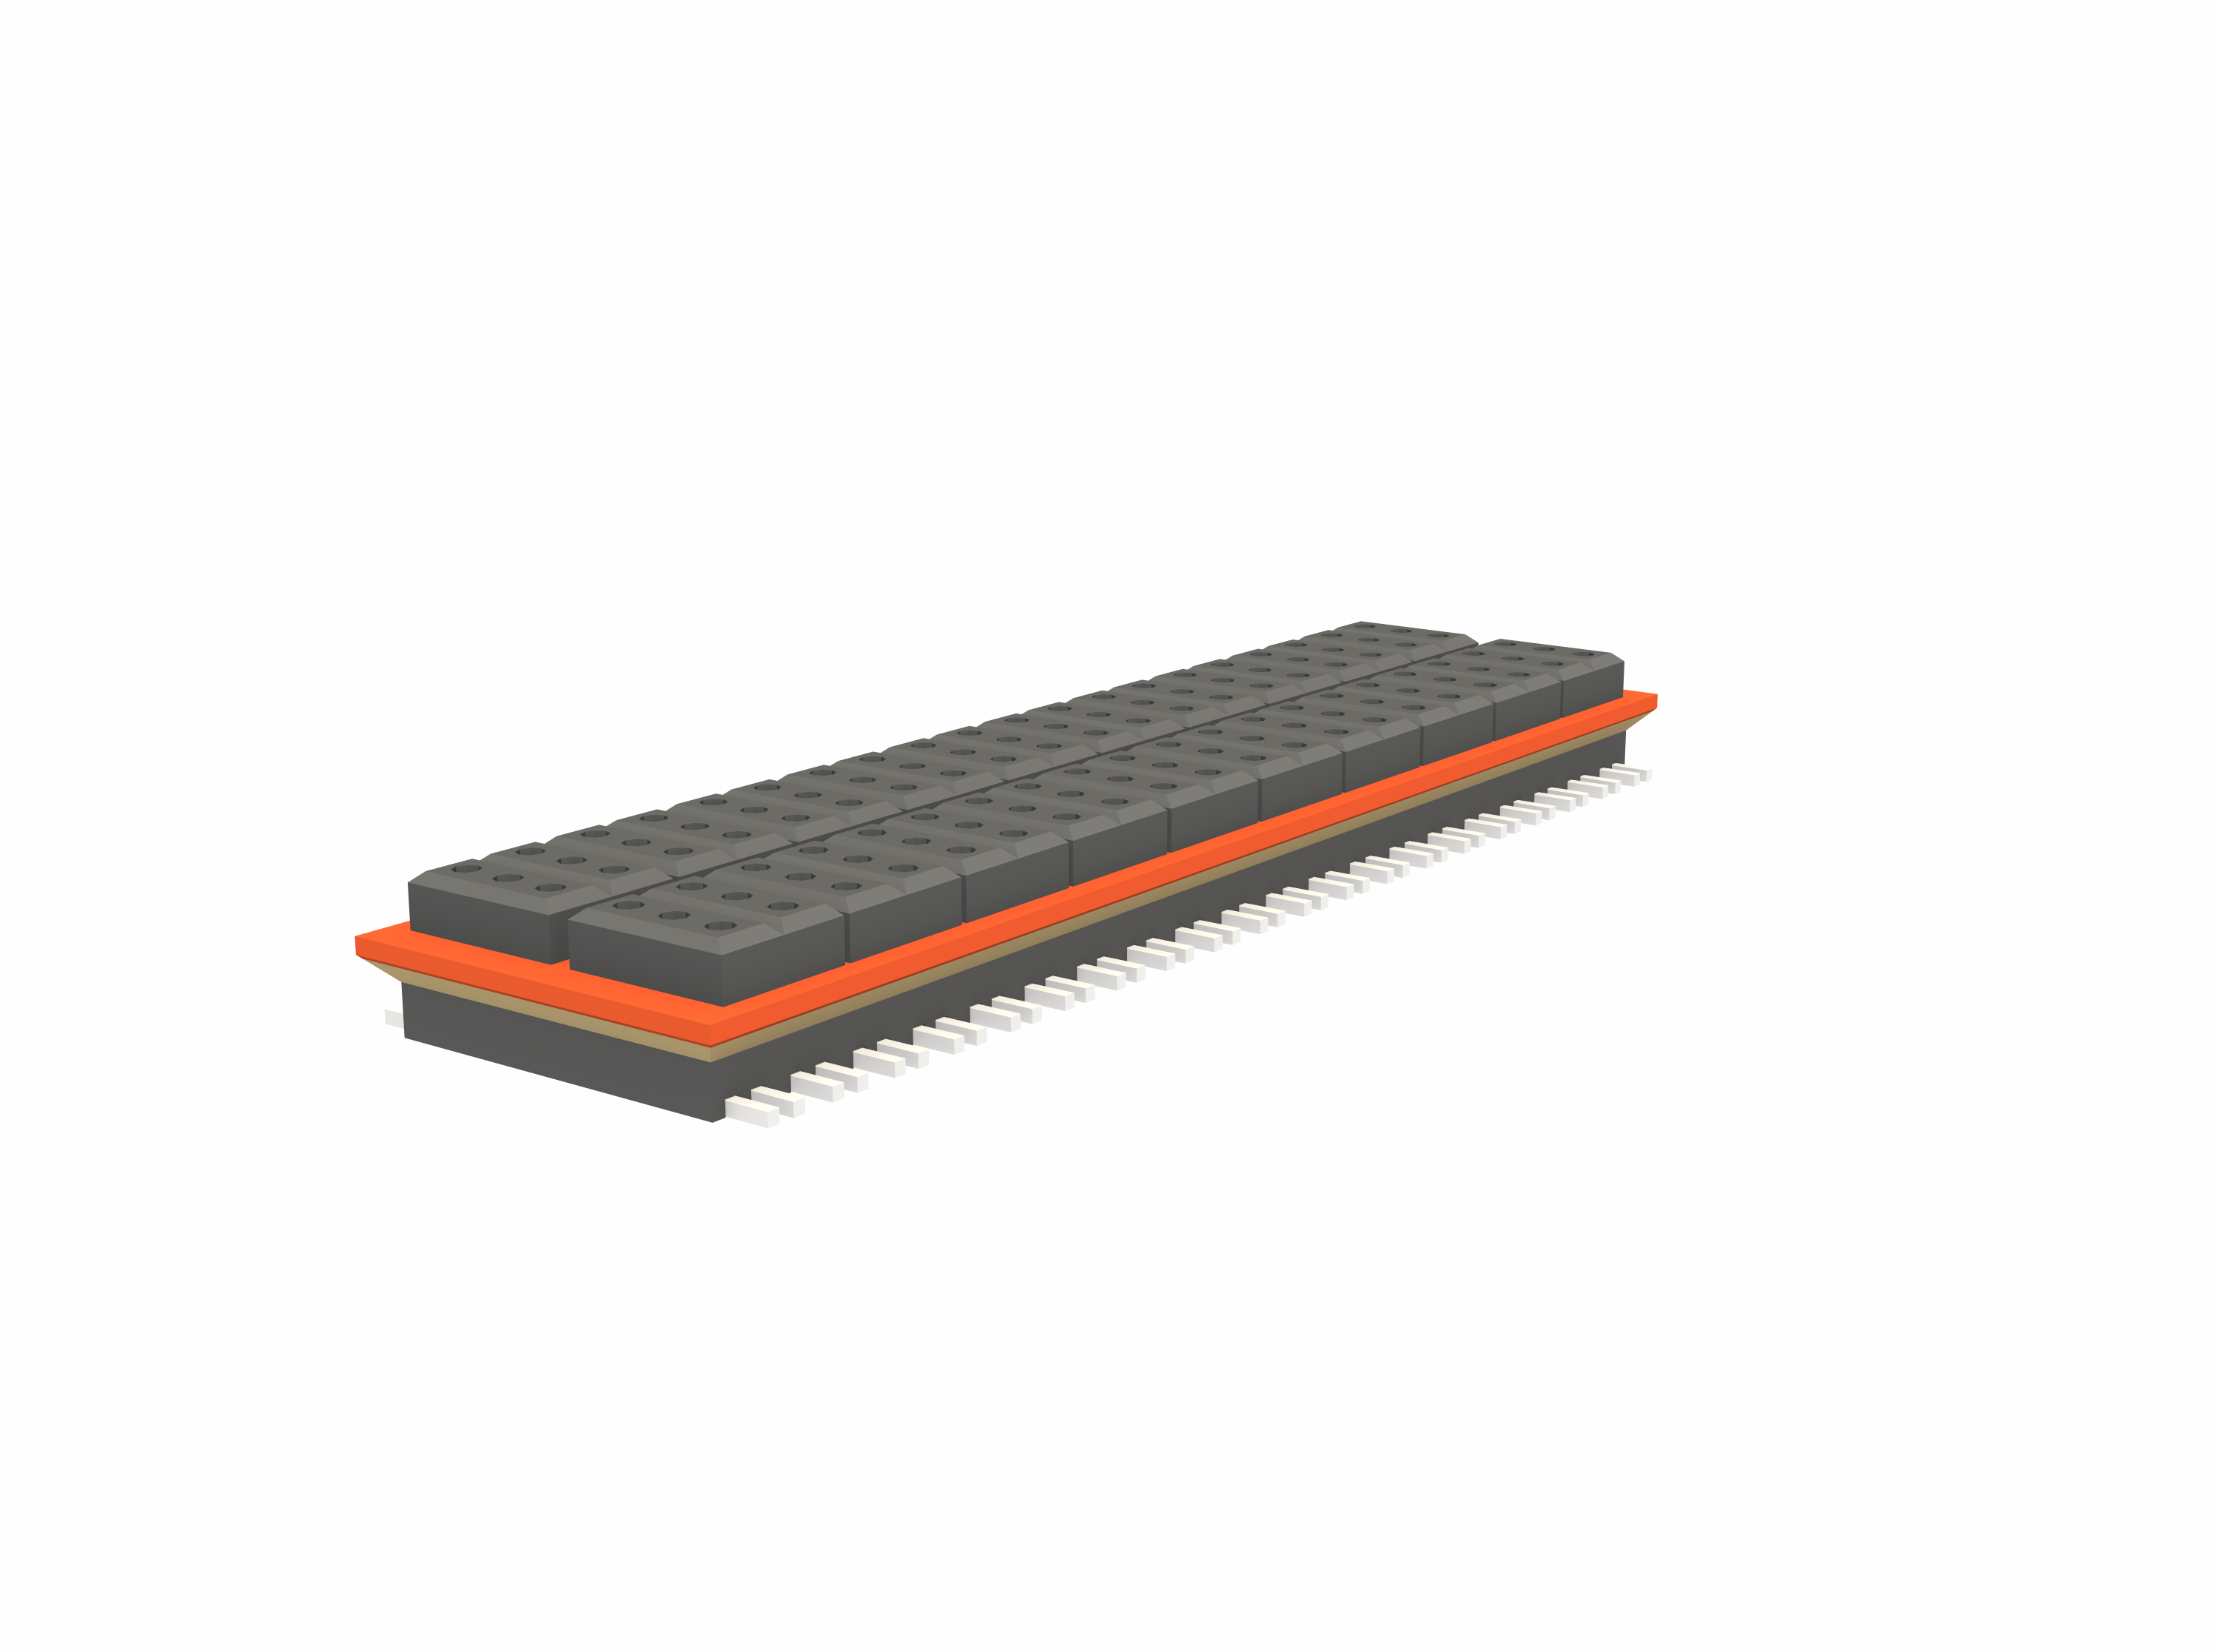
\includegraphics[width=\textwidth]{../media/populations/ap32-mesh-components/print/metal-bath-anodes-cathode-bus-bars.png}
      \caption{Éléments à proximité des fluides}
      \label{fig:ap32-geometry-elements}
    \end{subfigure}
%
    \begin{subfigure}[b]{0.49\textwidth}
      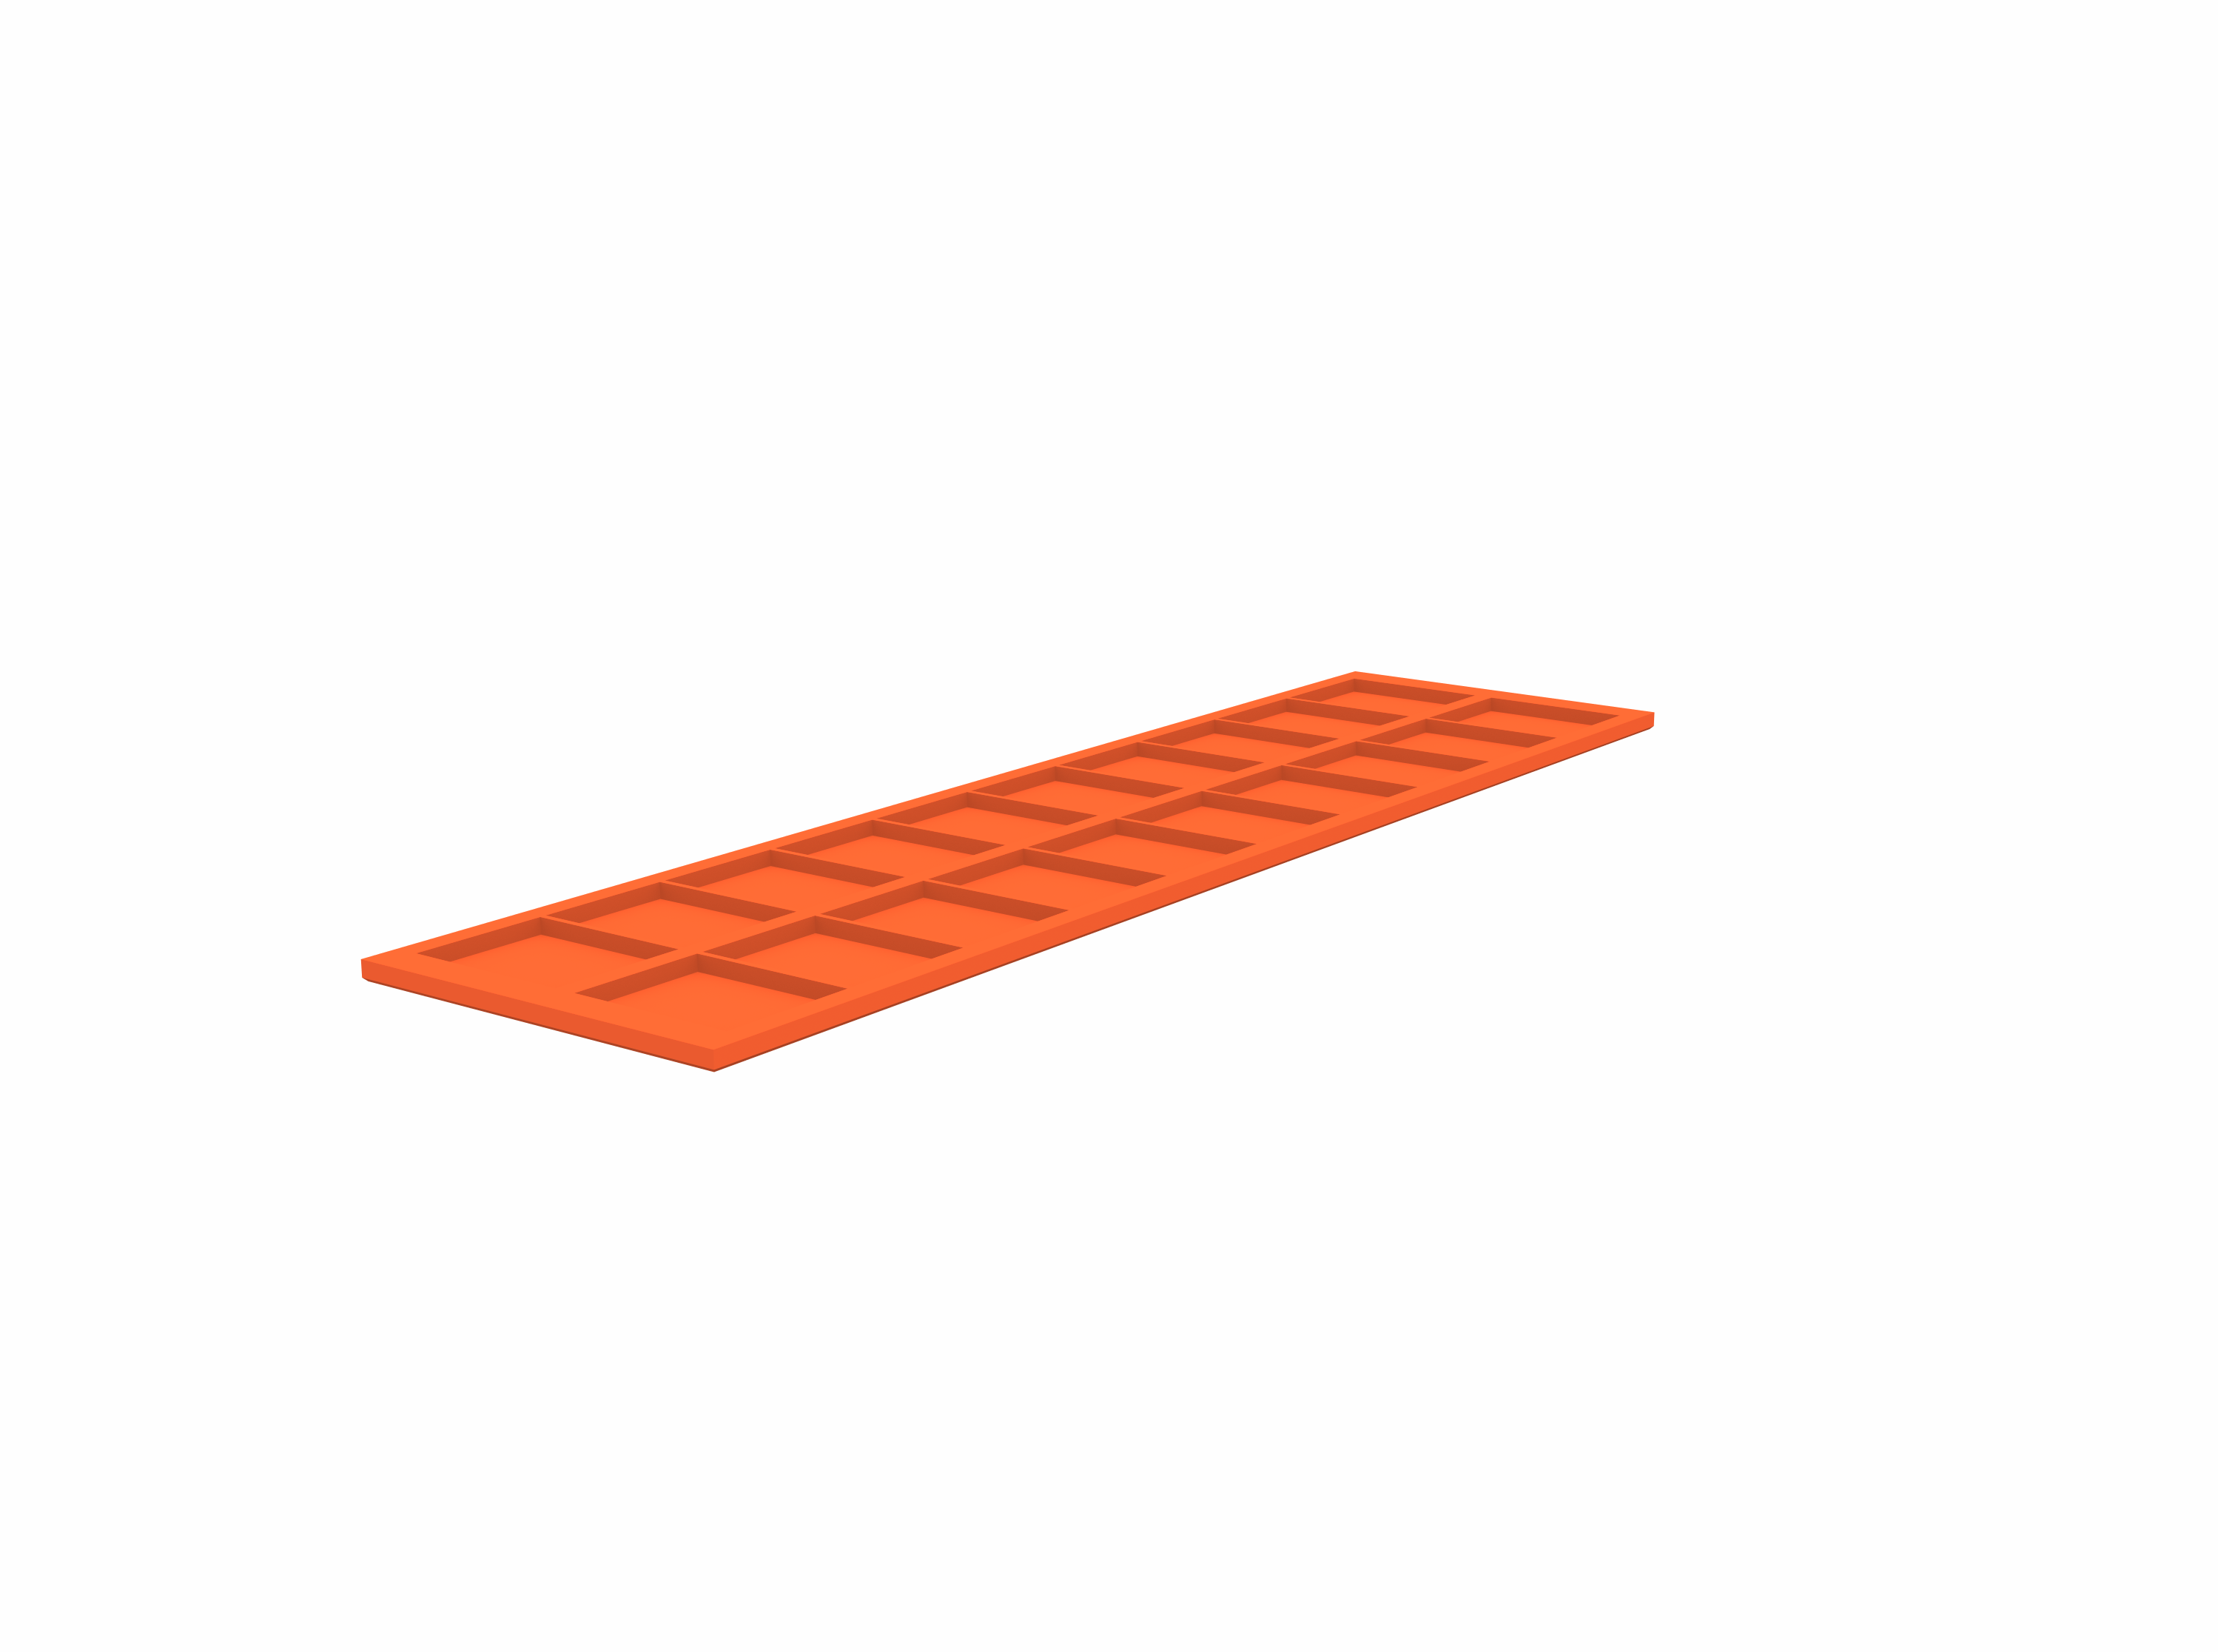
\includegraphics[width=\textwidth]{../media/populations/ap32-mesh-components/print/bath.png}
      \caption{Bain électrolytique}
      \label{fig:ap32-geometry-electrolyte}
    \end{subfigure}
%
    \caption{Géométrie des éléments importants à proximité
      du bain électrolytique dans une cuve AP32
      (fig. \ref{fig:ap32-geometry-elements}), et détail du volume
      occupé par le bain électrolytique dans cette même cuve
      (fig. \ref{fig:ap32-geometry-electrolyte}). On distingue
      les anodes en haut et la cathode
      en bas (\textbf{noir}), le bain électrolytique
      (\textbf{orange}), le métal liquide (\textbf{jaune}) et les
      bus bar (\textbf{gris clair}).}
    \label{fig:ap32-geometry}
  \end{center}
\end{figure}

Le plan anodique est composée de deux rangées de 10 anodes chacune,
représentées en noir sur la figure \ref{fig:ap32-geometry-elements}. La
surface du plan anodique est d'environ \num{40.3} \si{\square\meter}
et seulement \num{25}\% de la surface du bain est libre, le reste
étant recouvert par les anodes. La cuve est conçue pour que
l'électrolyte soit traversé par un courant électrique total de $I = $
\num{320000} \si{\ampere}, ce qui correspond à une densité de courant
d'environ \num{0.8} \si{\ampere\per\square\centi\meter} à la surface
des anodes. En supposant un rendement de réaction de \num{100}\%, ce
courant électrique permet de réduire par électrolyse \num{29.8}
\si{\gram\per\second} ou \num{2577} \si{\kilo\gram} par jour
d'aluminium métallique, \ie, un peu plus qu'\num{1} \si{\cubic\meter}
de métal par jour. Cet accroissement de volume de métal correspond à
une variation de l'épaisseur du métal liquide d'environ \num{2}
\si{\centi\meter}.

Du coté des anodes, la réaction d'électrolyse produit environ
\num{0.8} \si{\mol\per\second} d'oxygène \ce{O2}. Cet oxygène réagit
immédiatement avec le carbone de l'anode pour former du \ce{CO2}. Dans
l'ensemble de la cuve, l'électrolyse produit au total environ \num{80}
\si{\liter} par seconde de gaz, qui remonte vers la surface du bain
par le canal central et les canaux latéraux. La réaction de l'oxygène
avec le carbone des anodes \footnote{L'oxydation du carbone qui
  constitue les anodes par l'oxygène qui résulte de la réaction
  d'électrolyse forme du \ce{CO2} sous forme gazeux.} provoque
l'érosion de celles-ci à une vitesse d'environ \num{1100}
\si{\kilo\gram} par jour. Étant donné le nombre total d'anodes et leurs
tailles respectives, chaque anode d'une cuve AP32 a une durée de vie
d'environ 30 jours, après quoi elle doit être remplacée par une anode
neuve.

Pour compenser l'alumine dissoute qui est consommée par la réaction
d'électrolyse, il faut injecter en moyenne au cours du temps $56.3$
\si{\gram\per\second} de poudre d'alumine. Comme déjà mentionné dans
la section \ref{sec:introduction-hall-heroult}, la poudre d'alumine
est déposée à la surface du bain dans le canal central par une série
d'injecteurs dont la position est fixe. Un piqueur vient percer
mécaniquement un trou dans la croûte et créer un accès à la surface
libre du bain avant chaque injection. Ce trou se rebouche rapidement,
et pour cette raison l'injection de la poudre d'alumine ne peut pas
avoir lieu continûment.

Pour maintenir un rendement énergétique maximum, éviter l'émission de
gaz fluorés et éviter l'occurence des effets d'anodes, il est crucial
que la concentration d'oxyde d'aluminium dissoute dans le bain soit
maintenue dans un intervalle très précis. Malheureusement, pour de
nombreuses raisons il est impossible de maintenir un bilan précis de
la quantité d'alumine dans le bain en fonction de ce qui est injecté
et de ce qui est consommé. En effet, l'environnement rend difficile la
mesure précise des quantités déposées, une partie des particules
volatiles ne parviennent jamais dans le bain, des agrégats se forment,
dont une partie s'accumule au fond de la cuve sur la cathode, et des
réactions chimiques parasites viennent, entre autres, grever ce bilan.

Pour contourner cette difficulté, les opérateurs exploitent le fait
que la resistivité du bain électrolytique dépend de la concentration
d'alumine dissoute, et atteint un minimum à la concentration optimale
$\concentration \approx$ \num{3}\% masse. En mesurant la chute de
potentiel électrique à travers le bain électrolytique, on maintient la
concentration d'alumine dissoute au voisinage de la concentration
optimale en alternant une phase de sur-alimentation en alumine et une
phase de sous-alimentation. Durant la phase de sur-alimentation, la
concentration d'alumine va passer au-delà de la concentration optimale
et par conséquent accroître la resistivité du bain. Passé un certain
seuil, on débute une phase de sous-alimentation, durant laquelle la
résistivité commence par chuter, puis croît à nouveau. Passé un
certain seuil, on amorce une phase de sur-alimentation, et ainsi de
suite.

Dans chacune des phases de sur-alimentation ou sous-alimentation, les
injecteurs déposent les doses d'alumine selon une cadence préétablie
et périodique. La période et la taille des doses peuvent être spécifiées
indépendemment pour chaque injecteur.

\paragraph{Calcul de l'écoulement dans le bain} Une approximation de vitesse
d'écoulement du bain $u$ et de la densité de courant $j$ dans la cuve
AP32 est obtenue par l'intermédiaire du modèle multi-physique
stationnaire proposé par S. Steiner \cite{Steiner2009}, J. Rochat
\cite{Rochat2016} déjà introduit dans la section
\ref{sec:populations-introduction}. La figure \ref{fig:ap32-flow-acd}
représente la vitesse d'écoulement ainsi calculée par le logiciel
\citealucell{} dans le bain électrolytique de la cuve AP32, dans
l'ACD. Lorsque la densité de courant électrique est répartie
uniformément sur toutes les anodes, l'écoulement dans les fluides
forme deux tourbillons principaux qui tournent en sens opposés. Deux
petits tourbillons se forment dans les coins avals. Les vitesses
maximales de l'écoulement (\num{5} \si{\centi\meter\per\second}
environ) sont atteintes dans le canal central au niveau des extrémités
de la cuve, ainsi que le long de la paroi amont, de part et d'autre de
la cuve. Dans le reste du bain, et en particulier sous les anodes, la
vitesse d'écoulement dépasse rarement \num{2}
\si{\centi\meter\per\second}. La figure
\ref{fig:ap32-flow-streamlines} illustre les lignes de courant de
l'écoulement dans le bain. On remarque les lignes de courant
s'engagent dans les canaux latéraux et dans le bain en
pourtour des rangées d'anodes.

\paragraph{Conditions sur l'injection et l'effet Joule}
Le schéma numérique proposé dans la section
\ref{sec:populations-discretisation} est conçu de manière à conserver
exactement d'une part la masse d'alumine dans les populations de
particules $\population$ et concentration d'alumine dissoute
$\concentration$, et d'autre part la quantité d'énergie thermique liée
à la température du bain $\temperature$. Pour des raisons déjà
évoquées, ces bilans ne sont pas exactement respectés dans une cuve
industrielle réelle, et il faut en général injecter un peu plus d'alumine
que ce qui est consommé par la réaction d'électrolyse. Quand à
l'énergie thermique, nous avons supposé que le bain est isolé
thermiquement, alors que dans une cuve réelle une quantité non
négligeable d'énergie s'échappe par le métal, les parois latérales de
la cuve, les anodes, la surface du bain et par le \ce{CO2} qui
s'échappe dans l'atmosphère.

\begin{figure}[h!]
  \begin{center}
    \begin{tikzpicture}
      \begin{axis}[
          hide axis,
          colorbar,
          scale only axis,
          height=0.41\rasterimagewidth,,
          width=\rasterimagewidth,
          colorbar horizontal,
          point meta min=0.00,
          point meta max=0.05,
          colorbar style={
            title=Vitesse $u$ [\si{\meter\per\second}],
            width=7.4cm,
            height=0.3cm,
            xtick={0.00, 0.01, 0.02, 0.03, 0.04, 0.05},
            xticklabel style={
              /pgf/number format/fixed,
              /pgf/number format/fixed zerofill,
              /pgf/number format/precision=2
            },
            scaled x ticks = false,
            at={(0.5\rasterimagewidth,0.4cm)},
            anchor=north
          }
        ]
        \addplot [] coordinates {(0,0)};
        \node (myfirstpic) at (0,0) {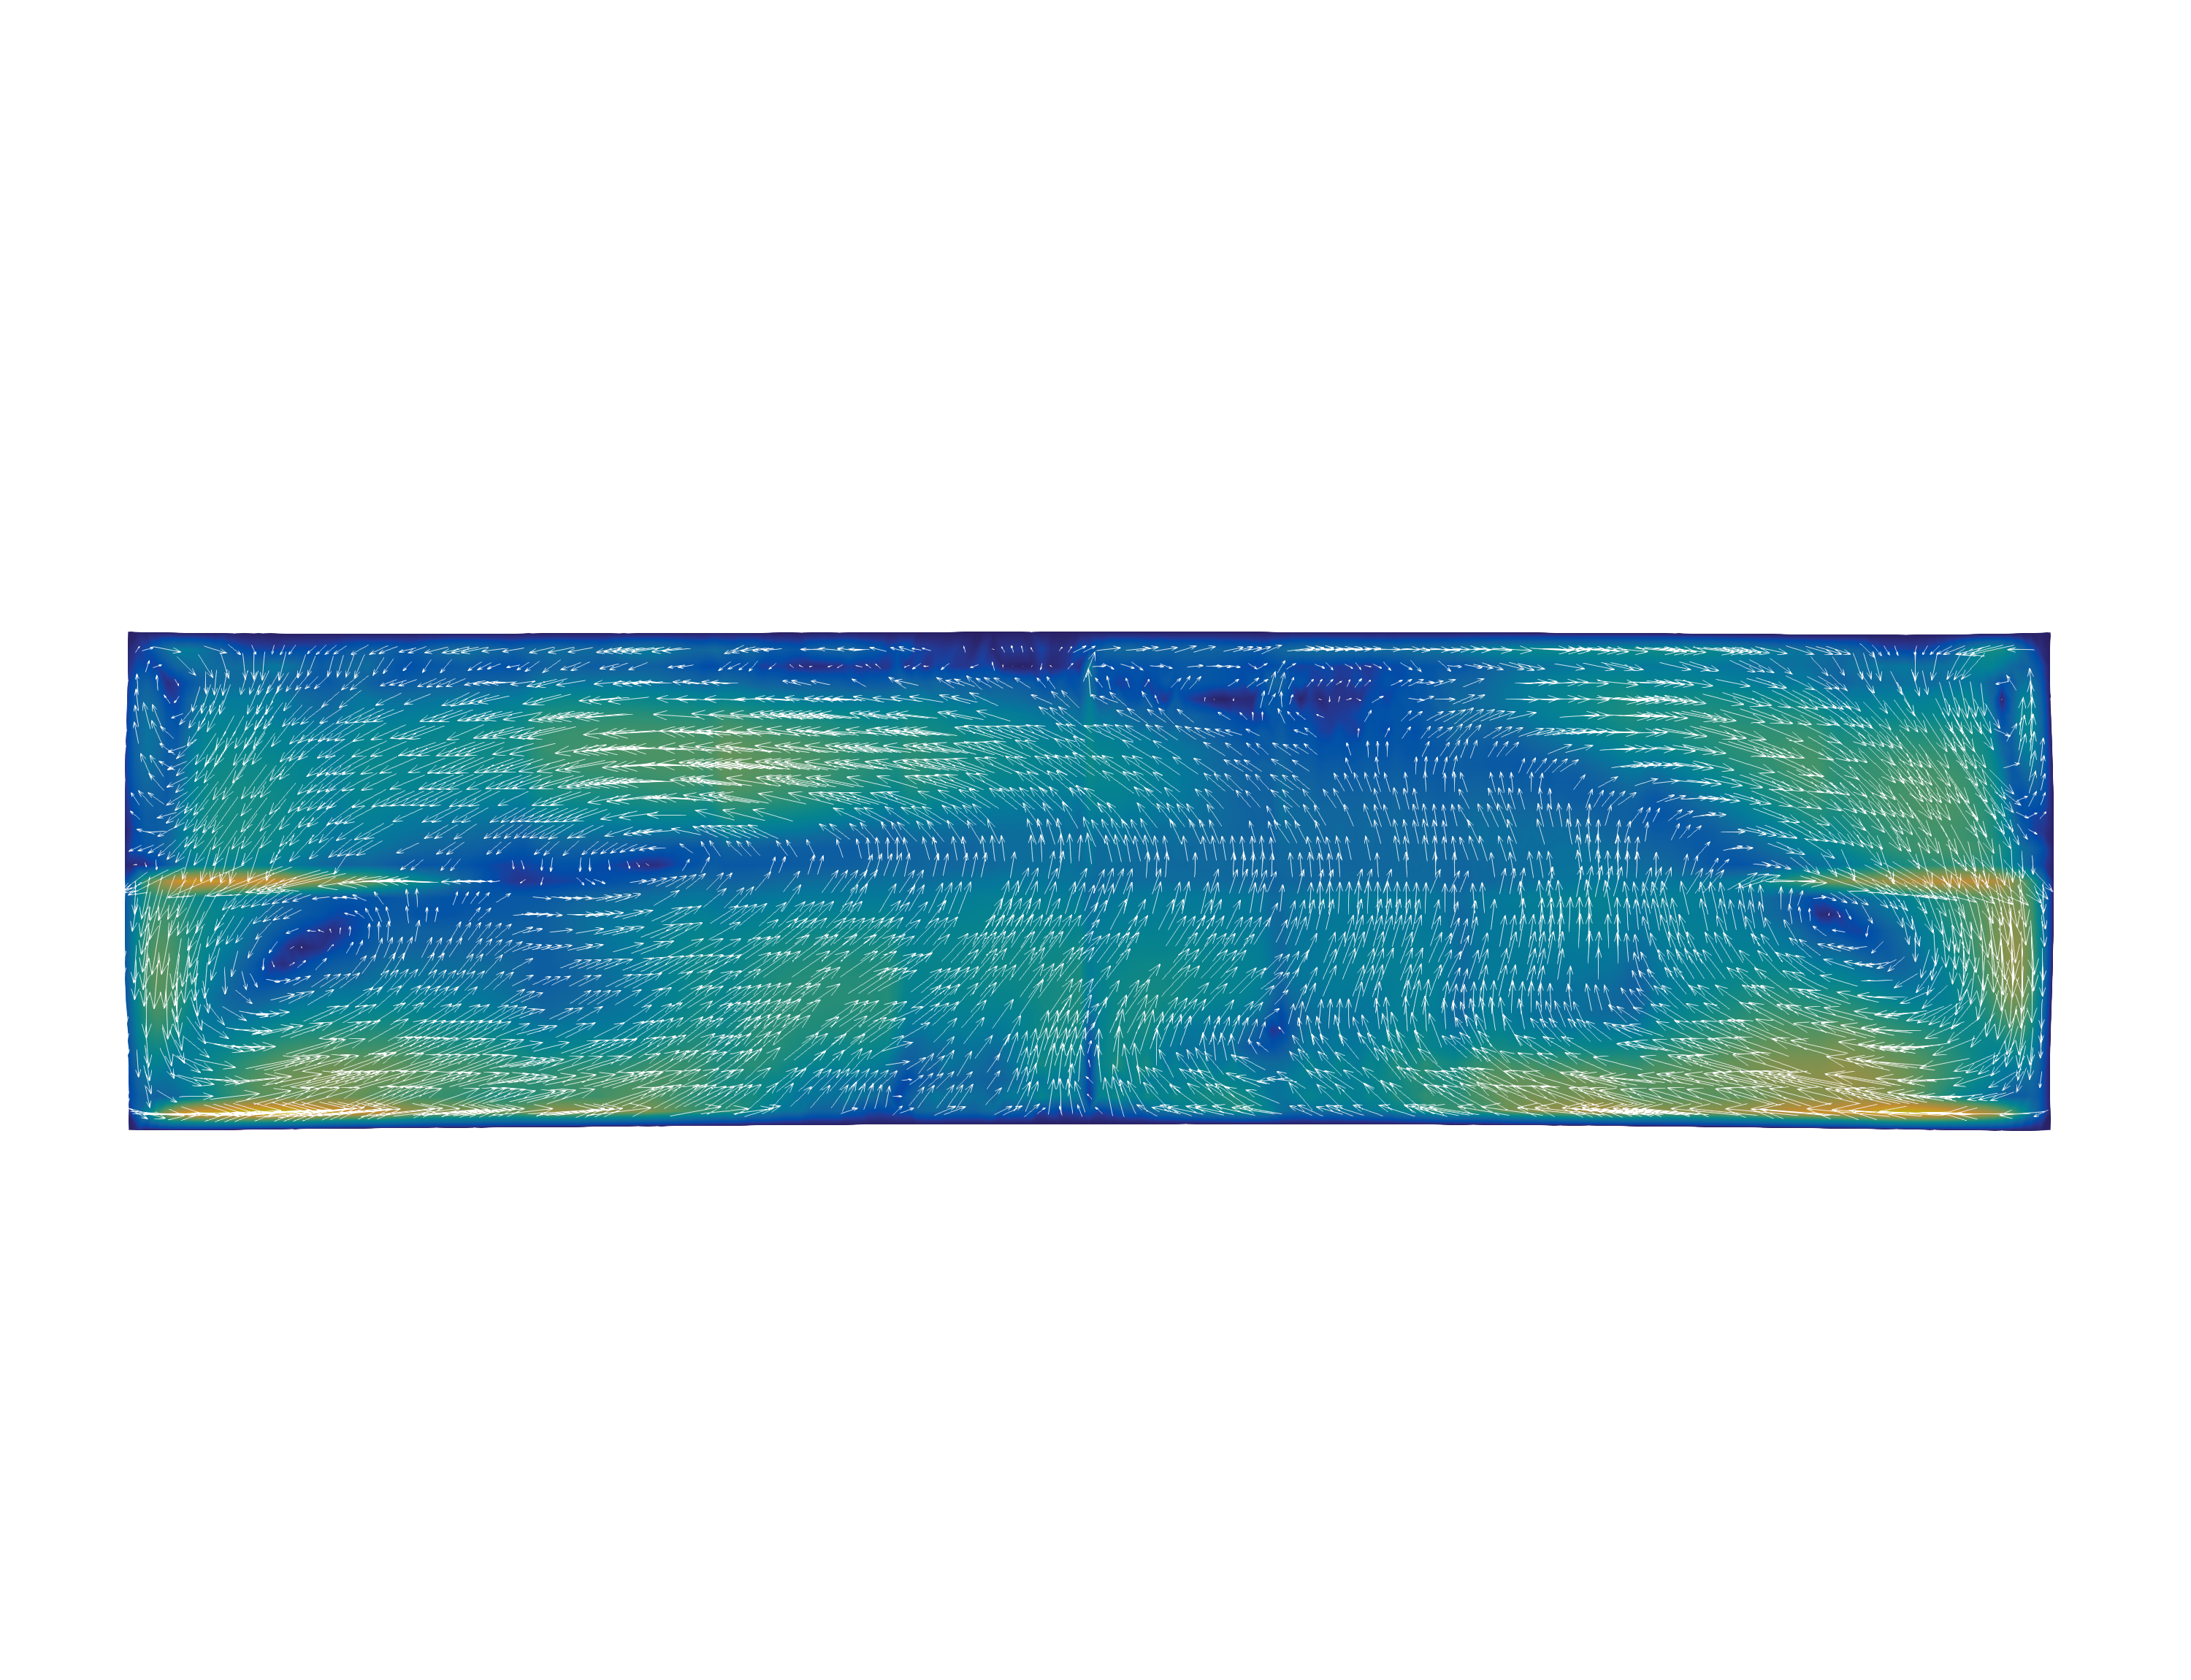
\includegraphics[width=\rasterimagewidth]{{../media/populations/ap32-fluid-flow/print/acd-all-anodes-velocity-0.00-0.05}.png}};
      \end{axis}
    \end{tikzpicture}
    \caption{Champ de vitesse $u$ dans le bain électrolytique d'une
      cuve AP32 restreint sur une surface placée à mi-hauteur de
      l'ACD, vue depuis dessus. Cette situation correspond à un état
      d'opération standard.}
    \label{fig:ap32-flow-acd}
  \end{center}
\end{figure}

\begin{figure}[h!]
  \begin{center}
    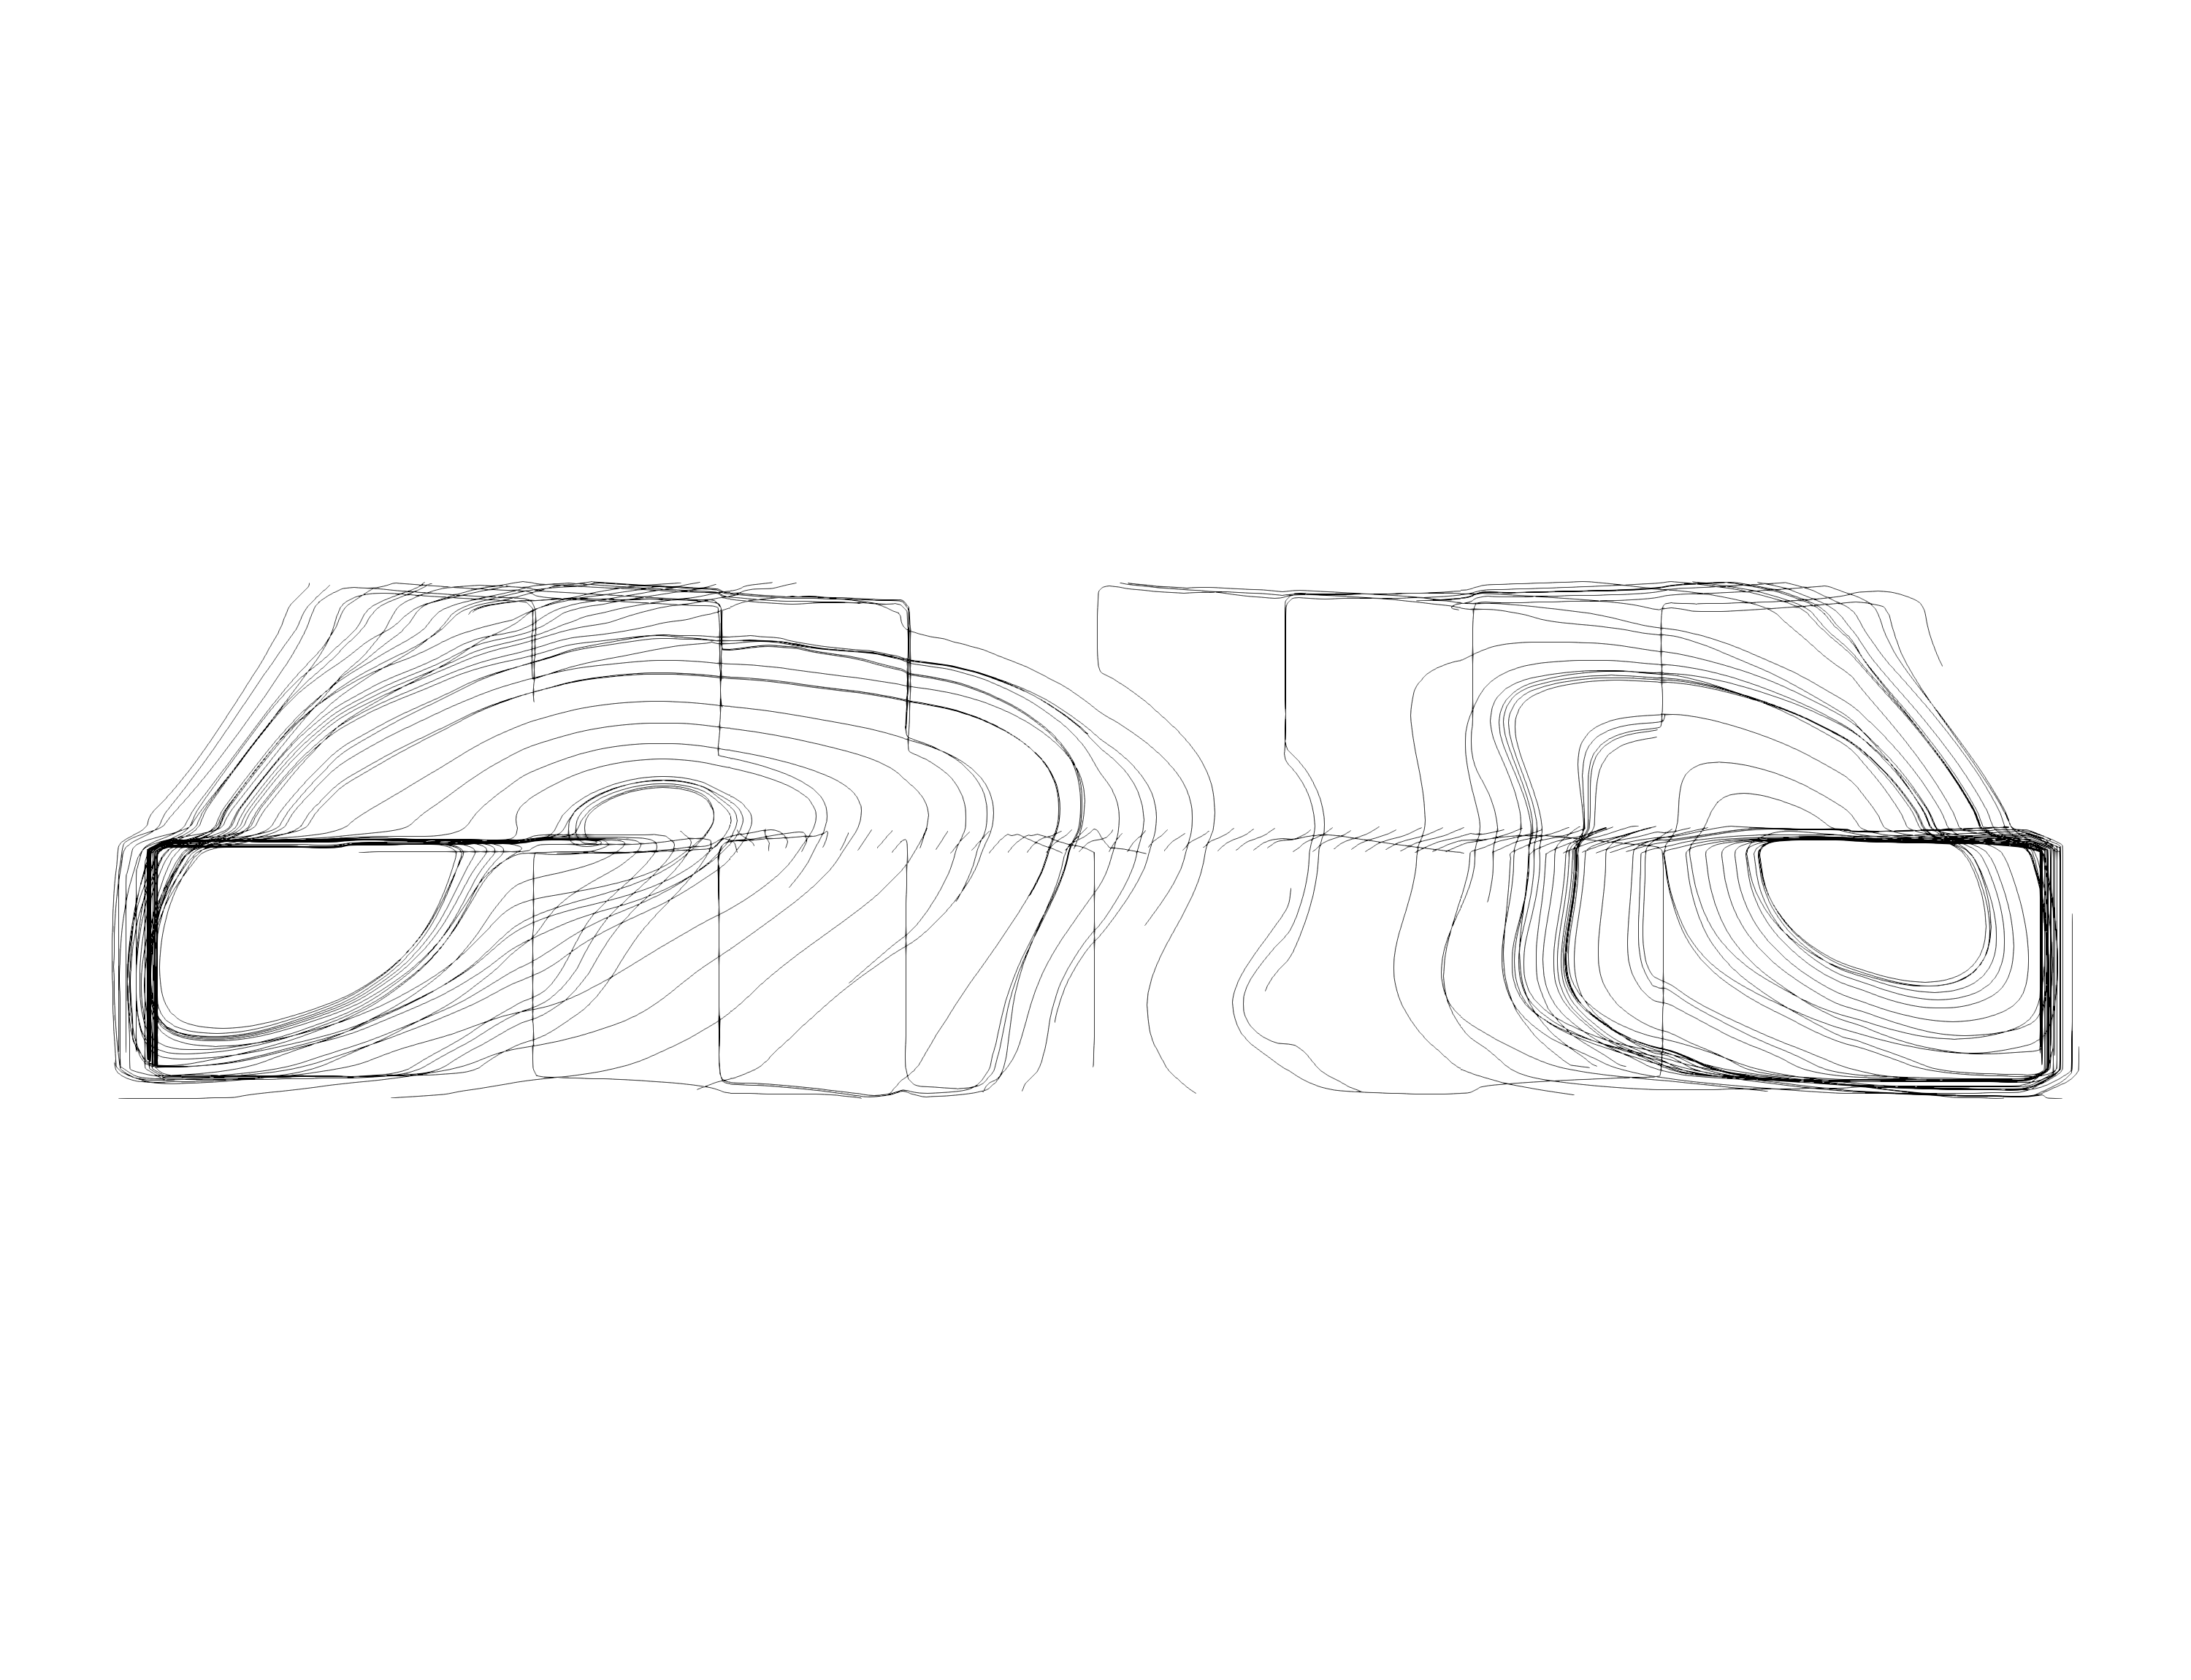
\includegraphics[width=\rasterimagewidth]{../media/populations/ap32-fluid-flow/print/chanel-velocity-streamlines.png}
    \caption{Lignes de courant correspondant au champ de vitesse
      représenté sur la figure \ref{fig:ap32-flow-acd}. Les lignes de
      courant prennent leur origine le long du canal central.}
    \label{fig:ap32-flow-streamlines}
  \end{center}
\end{figure}

Pour éviter que la masse totale d'alumine dans la cuve croisse sans
limite au cours du temps, il faut s'assurer que dans un état pseudo
stationnaire, la masse d'alumine reste proche de la masse d'alumine
initialement présente dans le bain. En d'autres termes, si $M_n$ est
la masse totale d'alumine dans le bain à l'instant $t_n$ telle que
définie dans la section (\ref{sec:populations-discretisation}), alors
on demande à ce que
\begin{equation*}
\lim_{n\to\infty} \frac{M_{n+1} - M_{0}}{t_n} = 0,
\end{equation*}
c'est-à-dire que
\begin{equation}\label{eq:injection-mass-condition}
  \frac{I[\cee{Al2O3}]}{6F}
  =\lim_{n\to \infty}\frac{1}{t_{n+1}}\ \sum_{\mathclap{\substack{k\\ i^k + 1\leq n +
        1}}}\ \int_\Omega\intd{x}\int_\rplus\intd{r}\aluminadensity S^k \frac{4}{3}\pi r^3.
\end{equation}
Il faut donc choisir la masse des doses d'alumine injectées $S^k$, $k
= 1, 2,\dots$ et les temps d'injection $\tau^k$, $k = 1,2,\dots$ de
sorte à ce que le débit de masse de poudre d'alumine moyen au cours du
temps soit égal à $\frac{I[\cee{Al2O3}]}{6F}$, c'est-à-dire
\num{56.382e-3} \si{\kilo\gram\per\second}.

La cuve AP32 possède 4 injecteurs placés au-dessus du canal central,
numérotés de 1 à 4, dans le sens de la coordonnée $x$ croissante (voir
la figure \ref{fig:anode-configuration}). Les paramètres qui
définissent chaque injecteur sont regroupés dans la table
\ref{tab:injectors}.

La masse des doses dans la table \ref{tab:injectors} est choisie de
telle sorte à ce que l'ensemble des 4 injecteurs injecte 25\% de la
masse d'alumine en moyenne. La région de répartition des densités des particules
initiales $S^k$ est décrite dans \cite{Hofer2011}. Plus précisément,
chaque quantité $S^k$ est une fonction lisse à support
compact centrée autour du point d'injection de l'injecteur
correspondant. La distribution initiale en rayon est approximée
par une loi log-normale basée sur des mesures expérimentales. Puisque
les rapport des périodes d'injection des 4 injecteurs sont des nombres
rationnels, on peut définir une période globale $P$ liée à l'ensemble des
4 injecteurs. Étant données les périodes d'injections reportées dans la table
\ref{tab:injectors}, le cycle d'injection global est périodique après une
transition initiale de \num{64}\si\second, avec une période
de $P = \num{192}$ \si\second. La figure \ref{fig:injections} représente les
injections qui ont lieu durant les \num{192} premières secondes de la
simulation.

\begin{figure}[h!]
  \begin{center}
    \input{../media/populations/anode-configuration/anode-configuration.pdf_tex}
    \caption{Vue schématique de la partie supérieure du bain
      électrolytique. Les blocs rectangulaires représentent
      l'emplacement des anodes, tandis que les cercles indiqués par
      les flèches et numérotés marquent l'emplacement des injecteurs
      disposés le long du canal central.}
    \label{fig:anode-configuration}
  \end{center}
\end{figure}

\begin{figure}[h!]
  \begin{center}
    \input{../media/populations/cadence/cadence.tex}
    \caption{Temps d'injections des différents injecteurs de la cuve
      AP32. Chaque cercle représente une injection. Chaque ligne
      correspond à l'un des 4 injecteurs.}
    \label{fig:injections}
  \end{center}
\end{figure}

\begin{table}[h!]
  \begin{center}
    \caption{Paramètres caractérisant les 4 injecteurs de la cuve AP32.}
    \label{tab:injectors}
    \begin{tabularx}{\textwidth}{@{}rrrrZ@{}}
      \toprule
      Injecteur & Position & Première injection & Intervalle d'injection & Masse de dose\\
      \midrule
      \#1         & \num{-4.4}\si\meter & \num{16}\si\second & \num{16}\si\second  & \num{0.225} \si{\kilo\gram} \\
      \#2         & \num{-1.6}\si\meter & \num{32}\si\second & \num{32}\si\second  & \num{0.451} \si{\kilo\gram} \\
      \#3         & \num{ 1.6}\si\meter & \num{48}\si\second & \num{48}\si\second  & \num{0.676} \si{\kilo\gram} \\
      \#4         & \num{ 4.4}\si\meter & \num{64}\si\second & \num{24}\si\second  & \num{0.338} \si{\kilo\gram} \\
      \bottomrule
    \end{tabularx}
  \end{center}
\end{table}

On détermine maintenant une condition sur la conductivité électrique
$\conductivity$, issue d'un argument similaire à celui fait sur
l'énergie thermique du bain. Pour que l'énergie thermique du bain
reste proche de l'énergie thermique initiale, on demande à ce que
\begin{equation}
  \lim_{n\to\infty}\frac{\electrolytedensity\electrolytehc\displaystyle\int_\Omega\parent{\temperature_{n+1}
    - \temperature_0}\intd{x}}{t_{n+1}} = 0,
\end{equation}
ce qui correspond à la condition, en considérant (\ref{eq:energy-mass-balance}):
\begin{eqnarray}
  \frac{1}{\conductivity} \int_\Omega j\cdot j\intd{x} &=&
  \aluminahc\parent{\tinit - \tinj}\lim_{n\to\infty}\frac{1}{t_{n+1}}\sum_{\mathclap{\substack{k\\ i^k +
  1 \leq n + 1}}}\int_\Omega\intd{x}\int_\rplus\intd{r}\aluminadensity
  \frac{4}{3}\pi r^3 S^k\nonumber \\
  &&-
       {\aluminadissolutionenthalpy}\lim_{n\to\infty}\frac{1}{t_{n+1}}\sum_{m = 0}^{n}\sum_{\mathclap{\substack{k\\ j^k < m + 1}}} \int_\Omega\intd{x}\int_\rplus\intd{r} \aluminadensity \frac{4}{3}\pi r^3\parent{n_{p,m+1}^k-n_{p,m}^k}.\nonumber\\
       \label{eq:energy-condition}
\end{eqnarray}
Le premier terme du membre de droite de (\ref{eq:energy-condition})
est égal à
\begin{equation*}
  \aluminahc\parent{\tinit-\tinj}  \frac{I[\cee{Al2O3}]}{6F}
\end{equation*}
en vertu de (\ref{eq:injection-mass-condition}). Pour que le deuxième
terme du membre de droite de (\ref{eq:energy-condition}) converge, il
est suffisant que chaque population $k\geq 1$ se dissolve en un temps
fini quelque soit $k$. Plus précisément, les populations $n_p^k$
se dissolvent en un temps fini s'il existe un entier positif $q'$ tel
que $n_{p,n}^k = 0$ pour tout $n > j^k + q'$.

Le cas échéant on peut télescoper la somme sur $k$ et en remarquant que
\begin{equation*}
  \int_\Omega n_{p,j^k}^k\intd{x} = \int_\Omega S^k\intd{x}
\end{equation*}
pour tout $k \leq 1$ et pour tout $r > 0$ lorsque la vitesse de chute
est nulle, le deuxième terme du membre de droite de
(\ref{eq:energy-condition}) se réduit à
\begin{equation*}
  {\aluminadissolutionenthalpy}\lim_{n\to\infty}\frac{1}{t_{n+1}}\sum_{\mathclap{\substack{k\\ i^k +
  1 \leq n + 1}}}\int_\Omega\intd{x}\int_\rplus\intd{r}\aluminadensity
  \frac{4}{3}\pi r^3 S^k.
\end{equation*}
Ainsi finalement,
\begin{equation*}
  \frac{1}{\sigma}\int_\Omega j\cdot j\intd{x}
  =\aluminahc\parent{\tinit-\tinj}\frac{I[\cee{Al2O3}]}{6F} + {\aluminadissolutionenthalpy}\frac{I[\cee{Al2O3}]}{6F}
\end{equation*}
et on fixe $\conductivity$ de sorte à satisfaire cette dernière
relation, c'est-à-dire que
\begin{equation}\label{eq:conductivity-condition}
  \conductivity = \frac{\displaystyle\int_\Omega j\cdot j\intd{x}}{\parent{\aluminahc\parent{\tinit-\tinj} + {\aluminadissolutionenthalpy} }
    \displaystyle\frac{I[\cee{Al2O3}]}{6F}}.
\end{equation}

\paragraph{Diffusivité du bain électrolytique} La vitesse d'écoulement
stationnaire du bain $u$ obtenue par la méthode introduite dans
\cite{Steiner2009}, \cite{Rochat2016} est la vitesse moyenne d'un
écoulement turbulent. Les structures turbulentes du fluide sont
décrites par un modèle de longueur de mélange de Smagorinsky
\cite{Rochat2016}. Dans le modèle de Smagorinsky, les structures
turbulentes de l'écoulement se traduisent par une viscosité de
l'écoulement moyen $u$ proportionnelle au tenseur des déformation de
$u$. Dans le présent travail, nous caractérisons la diffusivité
$\electrolytecdiff$ de la concentration $\concentration$ et la
diffusivité $\electrolytetdiff$ de la température $\temperature$ par
quatre réels positifs $\electrolytemoldiff_\temperature$, $\electrolyteturbdiff_\temperature$,
$\electrolytemoldiff_c$ et $\electrolyteturbdiff_c$ pour tout
$x\in\Omega$ de la manière suivante:
\begin{align}
  &\electrolytetdiff(x) = \electrolytemoldiff_\temperature +
  \electrolyteturbdiff_\temperature\parent{2\sum_{i,j}\straintensor_{ij}(u(x))\straintensor_{ij}(u(x))}^{1/2},\\
  &\electrolytecdiff(x) = \electrolytemoldiff_c +
  \electrolyteturbdiff_c\parent{2\sum_{i,j}\straintensor_{ij}(u(x))\straintensor_{ij}(u(x))}^{1/2},
\end{align}
où $\straintensor_{ij}$, $i, j = 1,2,3$ est le tenseur des déformation
de l'écoulement défini par
\begin{equation}
  \straintensor_{ij}(u) = \frac{1}{2}\parent{\frac{\partial u_i}{\partial
      x_j} + \frac{\partial u_j}{\partial x_i}}.
\end{equation}
Les valeurs du paramètre $\electrolytemoldiff$ associé à la diffusion
moléculaire et de $\electrolyteturbdiff$ associé à la diffusion
induite par les turbulences de l'écoulement, sont rapportées dans la
table \ref{tab:dissolution-physical-parameters}.


\begin{table}
  \begin{center}
    \caption{Paramètres physiques et paramètres liés à la cuve AP32
      qui interviennent dans le transport et la dissolution de poudre
      d'alumine.}
    \label{tab:dissolution-physical-parameters}
    \begin{tabularx}{\textwidth}{@{}lllX@{}}
      \toprule
      Quantité                              & Valeur              & Unités                               & Description \\
      \midrule
      $\electrolytedensity$                 & \num{2130}          & \si{\kg\per\cubic\meter}             & Masse volumique du bain électrolytique                          \\
      $\aluminadensity$                     & \num{3960}          & \si{\kg\per\cubic\meter}             & Masse volumique de l'oxyde d'aluminium                          \\
      $\electrolytehc$                      & \num{2945}          & \si{\joule\per\kilo\gram\per\kelvin} & Chaleur spécifique du bain électrolytique liquide               \\
      $\aluminahc$                          & \num{1200}          & \si{\joule\per\kilo\gram\per\kelvin} & Chaleur spécifique de l'oxyde d'aluminium                       \\
      $g$                                   & \num{9.81}          & \si{\meter\per\square\second}        & Accélération de la gravité terrestre                            \\
      $I$                                   & \num{320000}        & \si{\ampere}                         & Courant électrique total                                        \\
      $\faraday$                            & \num{96485.33}      & \si{\coulomb\per\mol}                & Constante de Faraday                                            \\
      $\faradayyield$                       & \num{0.945}         & []                                   & Rendement de Faraday de l'électrolyse                           \\\relax
      [\ce{Al2O3}]                          & \num{0.102}         & \si{\kilo\gram\per\mol}              & Masse molaire de l'oxyde d'aluminium                            \\
      $\tinit$                              & \num{1223}          & \si{\kelvin}                         & Température initiale du bain électrolytique                     \\
      $\tinj$                               & \num{423}           & \si{\kelvin}                         & Température d'injection des particules d'alumine                \\
      $\tliq$                               & \num{1218}          & \si{\kelvin}                         & Température du liquidus du bain électrolytique                  \\
      $\tcrit$                              & \num{1218.86}       & \si{\kelvin}                         & Température critique de dissolution dans le bain électrolytique \\
      $K$                                   & \num{0.5e-09}       & \si{\square\meter\per\second}        & Taux de dissolution des particules d'alumine                    \\
      $\aluminadissolutionenthalpy$         & \num{5.3e5}         & \si{\joule\per\kilo\gram}            & Enthalpie de dissolution de l'oxyde d'aluminium                 \\
      $\conductivity$                       & $\approx$ \num{900} & \si{\siemens\per\meter}              & Conductivité électrique du bain électrolytique                  \\
%     $\electrolytelaminarviscosity$        & \num{2e-3}          & \si{\kilo\gram\per\meter\per\second} & Viscosité laminaire du bain électrolytique                      \\
%     $\electrolyteturbulentviscosity$      & \num{2e-3}          & \si{\kilo\gram\per\meter\per\second} & Viscosité turbulente du bain électrolytique                     \\
      $\electrolytemoldiff_\temperature$    & \num{5e-4}          & \si{\watt\per\kelvin\per\meter}      & Diffusivité thermique dans le bain                              \\
      $\electrolyteturbdiff_\temperature$   & \num{5e-4}          & \si{\joule\per\kelvin\per\meter}     & Diffusivité thermique turbulente dans le bain                   \\
      $\electrolytemoldiff_\concentration$  & \num{5e-4}          & \si{\square\meter\per\second}        & Diffusivité moléculaire dans le bain                            \\
      $\electrolyteturbdiff_\concentration$ & \num{5e-4}          & \si{\square\meter}                   & Diffusivité turbulente dans le bain                             \\
      $\electrolyteviscosity$               & \num{2e-3}          & \si{\kilo\gram\per\meter\per\second} & Viscosité laminaire du bain électrolytique                      \\
      $\csat$                               & \num{1689.7}        & \si{\mol\per\cubic\meter}            & Concentration de saturation de l'alumine dissoute               \\
      $\csatwp$                             & \num{7.8}           & w\%                                  & Concentration de saturation de l'alumine dissoute               \\
      $\cinit$                              & \num{635.3}         & \si{\mol\per\cubic\meter}            & Concentration initiale de l'alumine dissoute                    \\
      $\cinitwp$                            & \num{3.0}           & w\%                                  & Concentration initiale de l'alumine dissoute                    \\
      \bottomrule
    \end{tabularx}
  \end{center}
\end{table}

\paragraph{Conditions initiales de la concentration et de la
  température} Les conditions initiales des populations de particules
$n_p^k$ sont données par la relation (\ref{eq:splitting-np1-init}). En
d'autres termes, aucune particule n'est présente dans le bain
électrolytique à $t = 0$.

On observe expérimentalement sur des cuves d'électrolyse industrielles
que celles-ci atteignent un état stationnaire périodique lié à la
période du cycle d'injection après un temps caractéristique de
transition. On observe typiquement l'établissement de cet état
périodique indirectement par des mesures de la résistivité électrique
de la cuve. Par analogie, dans le cadre du modèle de transport et
dissolution d'alumine nous nous attendons à ce que la densité de
particules $n_p$, la concentration $\concentration$ et la température
$\temperature$ atteignent asymptotiquement lorsque $t\to\infty$, un
état périodique de période $P$ identique à la période du cycle
d'injection global, soit \num{192} \si{\second} dans notre cas.

Il est clair que plus les conditions initiales pour $c$ et
$\temperature$ sont éloignées de l'état périodique
asymptotique, plus le temps nécessaire pour atteindre un tel état est
long. Par conséquent, nous choisissons des conditions initiales
uniformes en espace pour la concentration et la température, et qui
soient égales aux conditions optimales d'opération de la cuve AP32:
\begin{align*}
  & \concentration(0, x) = \cinit,\quad\forall x\in\Omega,\\
  & \temperature(0, x) = \tinit,\quad\forall x\in\Omega.
\end{align*}
où $\cinit$, $\tinit$ sont donnés dans la table
\ref{tab:dissolution-physical-parameters}. Remarquons que la
concentration initiale $\cinit$ en \si{\mol\per\cubic\meter} s'exprime
en fonction de la concentration initiale
$\concentration_{\text{init},\%\mathrm w}$ en \% masse à l'aide de la
formule:
\begin{equation*}
  \cinit = \frac{\cinitwp \cdot
    100^{-1}}{\electrolytedensity[\cee{Al2O3}]\parent{1 - \cinitwp\cdot
      100^{-1}\parent{1 - \displaystyle\frac{\electrolytedensity}{\aluminadensity}}}}.
\end{equation*}
Nous exploiterons également cette dernière formule pour convertir les
valeurs du champ de concentration en \% masse lors de la visualisation
des résultats. Les deux valeurs de la concentration initiale selon les
unités physique sont rapportées dans la table
\ref{tab:dissolution-physical-parameters}.
% paramètres numérique. (deltat, maillage, deltar, N_r)

\paragraph{Paramètres de discrétisation}
Le maillage du domaine $\Omega$ est obtenu en même temps que les
champs $u$ et $j$ par la méthode déjà évoquée plus haut proposée par
\cite{Steiner2009}, \cite{Rochat2016}. On peut voir sur la figure
\ref{fig:bath-mesh} un aperçu du maillage de $\Omega$ qui correspond à
l'une des extrémités de la cuve. Le maillage est fortement anisotrope,
avec des rapports d'aspect d'environ \num{25} dans l'ACD. Le diamètre
des mailles est compris entre \num{38} \si{\centi\meter} (aux
extrémités de la cuve) et \num{9} \si{\centi\meter} (dans l'ACD et les
canaux). Le maillage comporte \num{282240} éléments tetraédriques. On
choisit le nombre de discrétisation des rayons des particules $M = 5$
et $\dr = \num{40}$ \si{\micro\meter}. Enfin on fixe $\dt = 1$
\si{\second} et $T = \num{10000}$ \si{\second}, le temps auquel on
veut évaluer la concentration.

\begin{figure}[h!]
  \begin{center}
    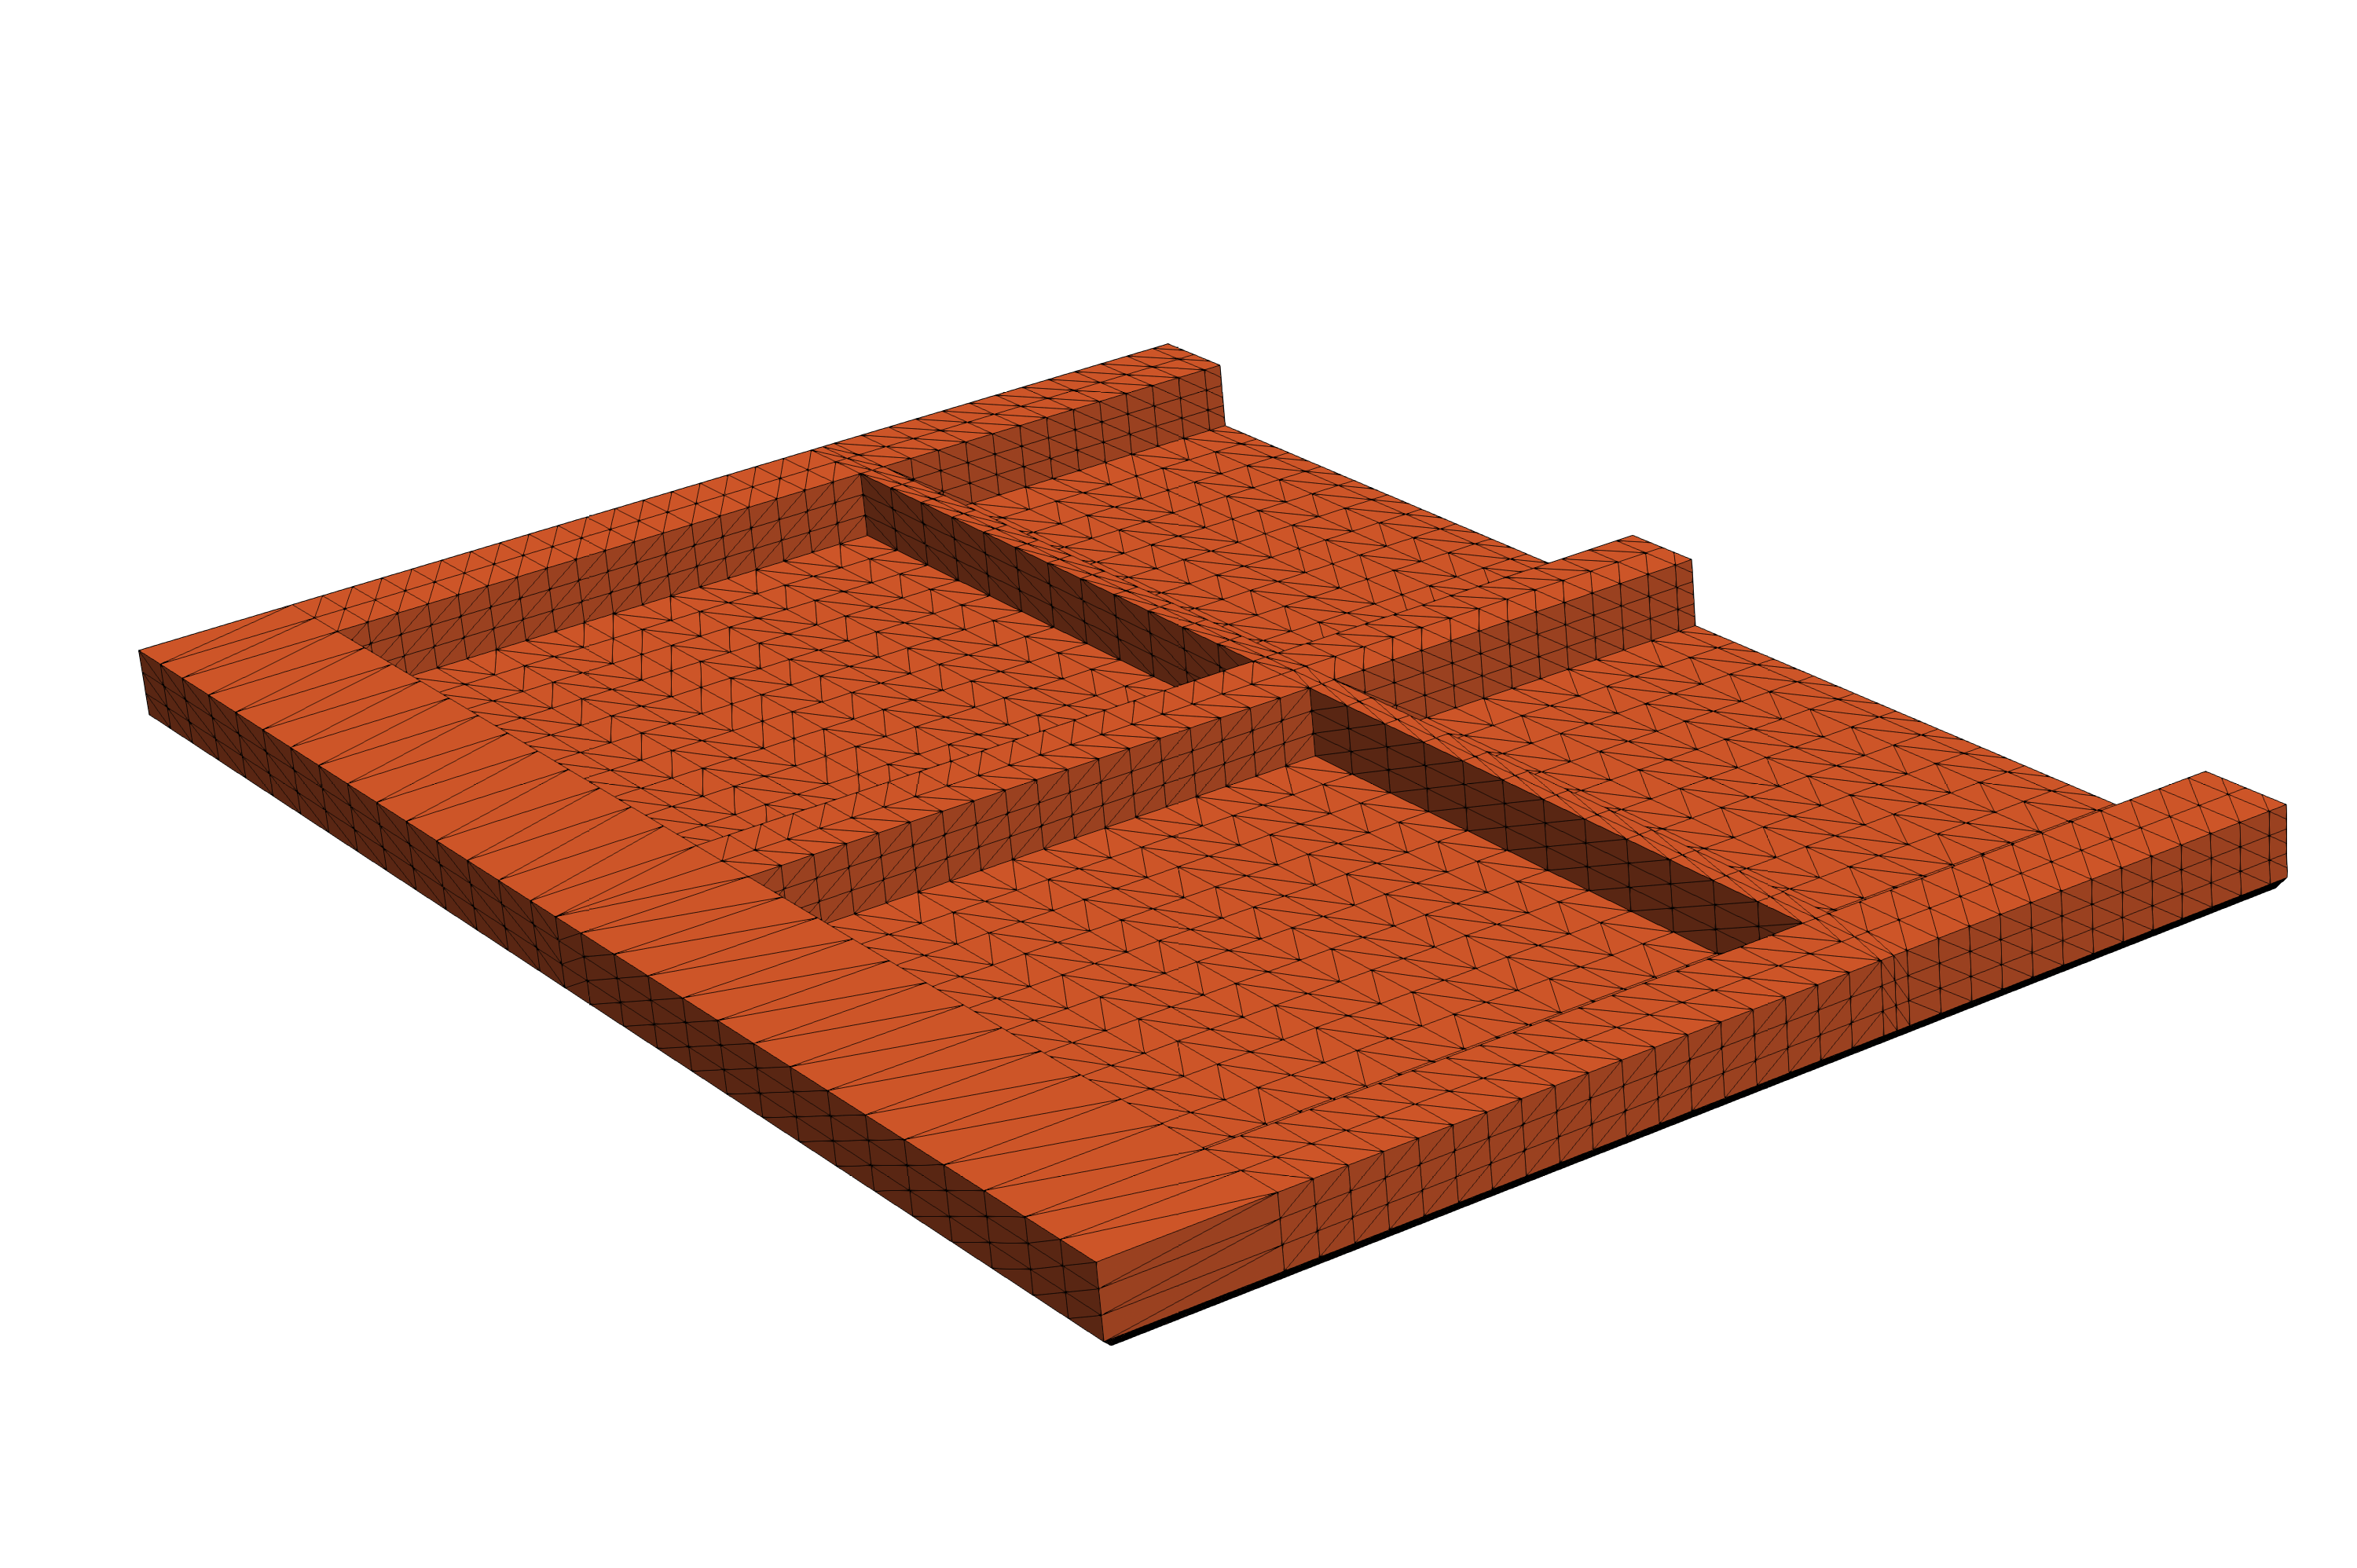
\includegraphics[width=\rasterimagewidth]{../media/populations/ap32-mesh-components/print/bath-mesh.png}
    \caption{Aperçu du maillage du domaine occupé par le bain
      électrolytique dans la cuve AP32.}
    \label{fig:bath-mesh}
  \end{center}
\end{figure}

\paragraph{Solution de référence} Afin d'évaluer l'effet de la
température de l'électrolyte sur la dissolution de la poudre
d'alumine, nous commençons par présenter un calcul qui tient compte
des hypothèses suivantes:
\begin{itemize}
\item les particules d'alumine ne chutent pas dans le bain ($w = 0$),
\item les particules commencent à se dissoudre instantanément, c'est-à-dire que $\tlat = 0$,
\item la vitesse de dissolution ne dépend pas de la température du
  bain $\temperature$. Plus précisément, la vitesse de dissolution
  définie par (\ref{eq:dissolution-rate}) est remplacée par
\begin{equation}
  \dissolutionrate(c, \temperature)= \left\{
  \begin{array}{ll}
    K\displaystyle\frac{\csat - \concentration}{\csat} &\quad \text{si } 0\leq
    \concentration \leq \csat,\\
    0& \quad \text{sinon}.
  \end{array}
  \right.
\end{equation}
\end{itemize}
Cette situation est équivalente à supposer que la température du
bain $\temperature$ reste largement supérieure à la température
critique $\tcrit$ au cours du calcul, de sorte à ce que le terme
exponentiel dans (\ref{eq:dissolution-rate}) soit proche de zéro.

Un des objectifs recherchés par les opérateurs de cuves
industrielles est de minimiser les écarts de concentration autour de
la concentration optimale d'alumine dissoute. Pour évaluer le champ
de concentration par rapport à cet objectif, nous proposons de
représenter la variance  du champ de concentration
$c$ dans $\Omega$ au cours du temps par:
\begin{equation}
  \Var_c(t) = \sqrt{\int_\Omega\parent{\concentration(t, x) - \bar \concentration(t)}^2\intd{x}},
\end{equation}
où $\bar \concentration$ est la moyenne de $\concentration$ sur
$\Omega$, c'est-à-dire
\begin{equation}
  \bar \concentration(t) = \frac{1}{\abs{\Omega}}\int_\Omega c(t, x)\intd{x}.
\end{equation}
Ici $\abs{\Omega}$ est le volume de $\Omega$. Clairement, la situation
idéale pour laquelle la concentration d'alumine est uniforme dans tout
l'électrolyte correspond à une variance de $\concentration$ nulle. A
l'inverse, plus $\concentration$ s'écarte de sa valeur moyenne, plus
sa variance est importante.

La valeur de $\Var_\concentration$ au cours du temps offre un moyen
d'évaluer si le système a atteint l'état périodique
recherché. En pratique on prend soin de
vérifier que la différence en norme $L^2$ à deux instants successifs
séparés par la période du cycle d'injection global $P$ est inférieure
à \num{1}\%. Pour tous les calculs présentés dans cette partie, la
solution satisfait ce critère pour $T = \num{10000}$ \si{\second}.

La figure \ref{fig:alumin-control-var} représente l'évolution de
la variance de la concentration au cours du temps. On remarque une
phase initiale lorsque $t\in[0,500]$, au cours de laquelle la variance
croît rapidement. Cette croissance ralentit quand la concentration
approche de l'état périodique, et à partir de $t \approx
\num{4500}$ \si{\second} nous pouvons considérer que la
concentration est dans un état périodique. Les
fluctuations de $\Var_\concentration$ que l'on peut observer sur la
figure \ref{fig:alumin-control-var} sont dues aux injections de poudre
d'alumine dans le bain. Immédiatement après l'injection, la
dissolution des particules provoque un accroissement rapide de la
concentration d'alumine dissoute localement autour du point
d'injection. Lorsque la dose est totalement dissoute, ce pique de
concentration est atténué par la diffusion de la concentration
dans l'électrolyte. Cet effet se traduit par un accroissement de la
variance de la concentration immédiatement après l'injection d'une
dose, puis par une décroissance de la variance.

\begin{figure}[h!]
  \begin{center}
    \input{../media/populations/variances/variance-control.tex}
    \caption{Évolution de $\Var_\concentration$ au cours du temps sur
      l'intervalle $[0, T]$ dans le bain électrolytique de la cuve
      AP32 lorsque la température n'est pas prise en compte dans la
      vitesse de dissolution des particules.}
    \label{fig:alumin-control-var}
  \end{center}
\end{figure}

Cependant, ces variations de la concentration dans l'état
périodique sont très localisées autour des points d'injection. Dans
le reste du bain électrolytique, les variations de la concentration
restent de l'ordre de \num{1}\%.

Puisque, lorsque l'état périodique est atteint, la
concentration varie peu au cours du cycle d'injection global, nous
pouvons nous permettre de visualiser la distribution de la
concentration dans le bain électrolytique à un instant arbitraire du
cycle d'injection global. Le temps $T = \num{10000}$ \si{\second}
auquel la solution est évaluée correspond donc à environ \num{51}
périodes du cycle d'injection global, sans compter la phase
transitoire initiale de \num{64} \si{\second}.

\begin{figure}{h!}
  \begin{center}
    \begin{tikzpicture}
      \begin{axis}[
          hide axis,
          colorbar,
          scale only axis,
          height=0.41\rasterimagewidth,,
          width=\rasterimagewidth,
          colorbar horizontal,
          point meta min=2.38,
          point meta max=4.21,
          colorbar style={
            title=Concentration $c$ [\%w],
            width=7.4cm,
            height=0.3cm,
            xtick={2.38, 3.00, 3.50, 4.00, 4.21},
            xticklabel style={
              /pgf/number format/fixed,
              /pgf/number format/fixed zerofill,
              /pgf/number format/precision=2
            },
            scaled x ticks = false,
            at={(0.5\rasterimagewidth,0.4cm)},
            anchor=north
          }
        ]
        \addplot [] coordinates {(0,0)};
        \node (myfirstpic) at (0,0) {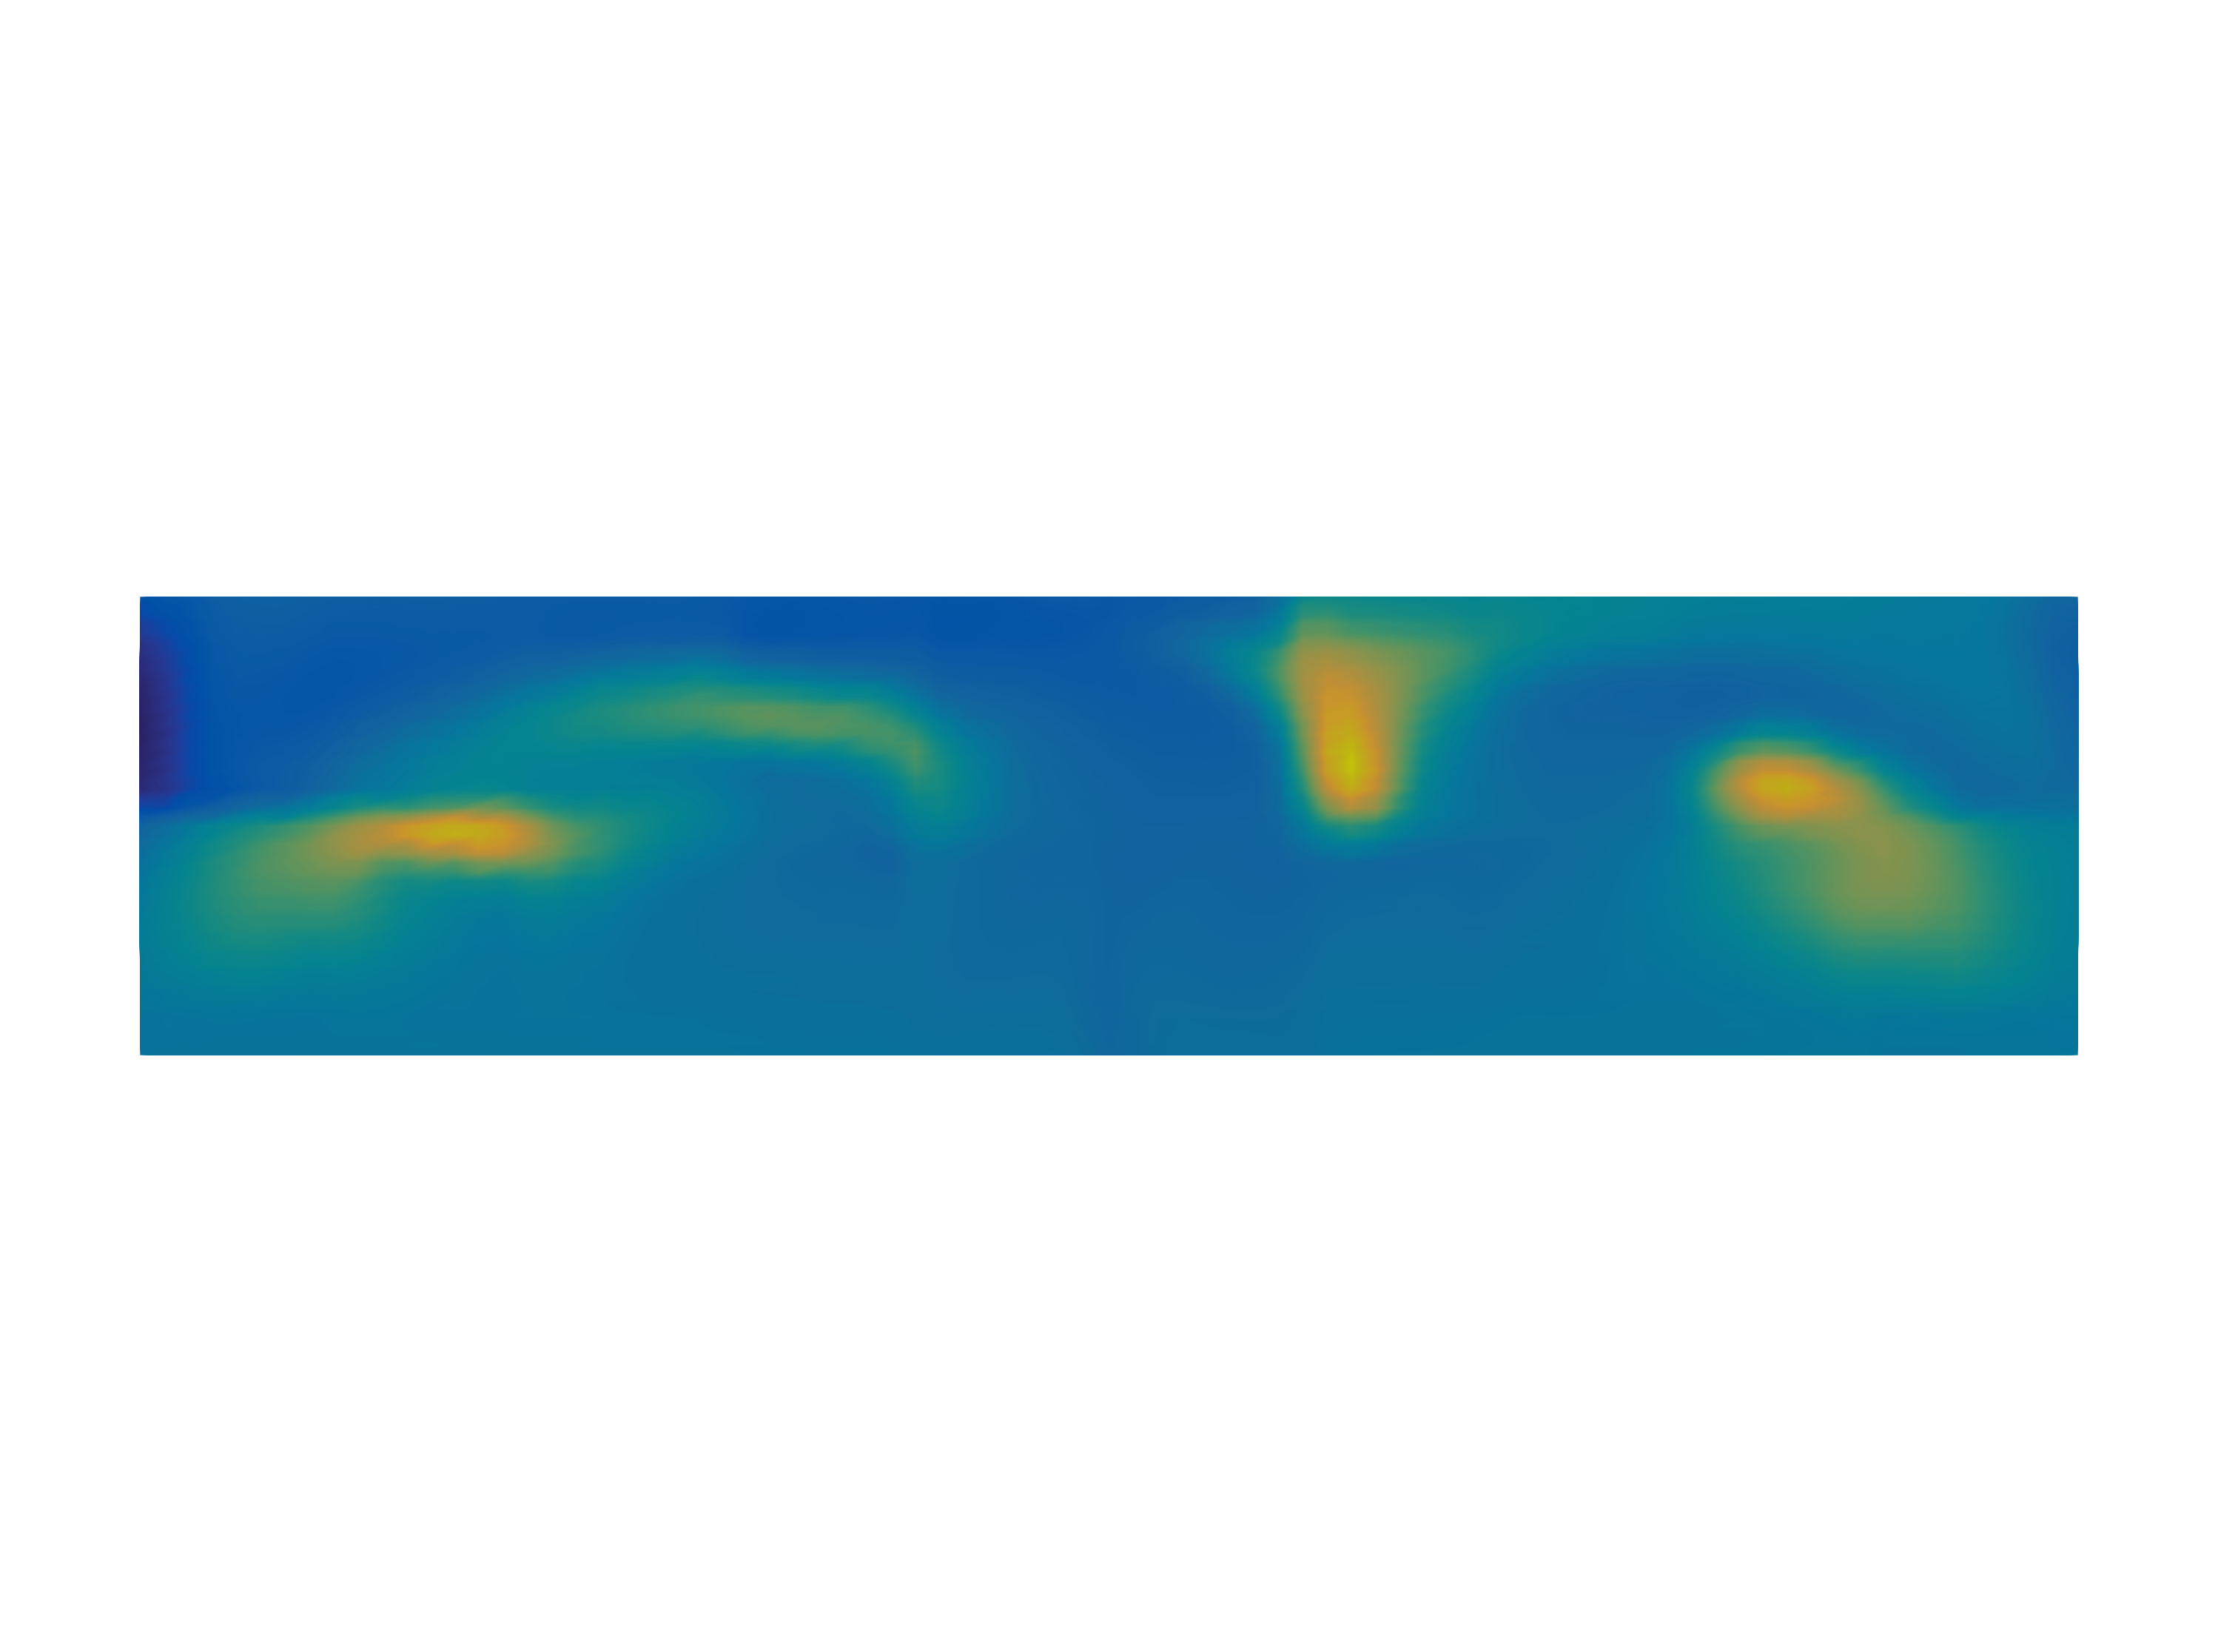
\includegraphics[width=\rasterimagewidth]{{../media/populations/application/print/alumina-control-2.38-4.21}.png}};
      \end{axis}
    \end{tikzpicture}
    \caption{Concentration d'alumine dissoute dans l'ACD de la cuve AP32 à $t =
      \num{10000}$ \si{\second} et à température constante.}
    \label{fig:ap32-alumina-wo-t}
  \end{center}
\end{figure}

On s'intéresse à la distribution de la concentration d'alumine là où a
lieu la réaction d'électrolyse, c'est-à-dire essentiellement dans
l'ACD. On se contente donc de visualiser la distribution de la
concentration d'alumine dans cette zone. Dans le domaine $\Omega$
occupé par l'électrolyte, l'ACD est maintenue constante avec $3.2$
\si{\centi\meter} d'épaisseur sur l'ensemble de l'interface. Pour
visualiser la concentration d'alumine dissoute dans l'ACD, on évalue
$\concentration$ sur une surface fictive placée dans l'électrolyte,
parallèle à l'interface et à une distance égale à la moitié de
l'ACD. La figure \ref{fig:ap32-alumina-wo-t} présente la distribution de la
concentration d'alumine dans le bain électrolytique.

On remarque sur la figure \ref{fig:ap32-alumina-wo-t} que la
concentration atteint des maxima locaux aux voisinages des points
d'injection, ce qui montre que l'essentiel de la poudre d'alumine se
dissout dans ces régions. Cette alumine dissoute est ensuite
transportée par l'écoulement. Les deux injecteurs de gauche alimentent
le tourbillon de gauche (voir figure \ref{fig:ap32-flow-acd}), tandis que les deux injecteurs de droite
alimentent essentiellement le tourbillon de droite. Les régions du bain
sous-alimentées sont les coins en aval, où la concentration descend
en dessous de \num{3} \%w et où l'écoulement est
caractérisé par la présence de petits tourbillons isolés. La région
centrale en amont des points d'injections est remarquablement uniforme
avec une concentration proche de \num{3} \%w.


Nous consacrons maintenant le reste de cette partie au
modèle de transport et dissolution d'alumine qui dépend de la
température du bain dans le bain de la cuve AP32, et l'on étudie
l'influence des nouveaux paramètres que ce modèle introduit,
en particulier le temps de latence $\tlat$, la température initial du
bain $\tinit$, la température critique $\tcrit$ et la vitesse de
chute des particules dans le bain $w$.


% Sensibilité par rapport a la latence de dissolution
\paragraph{Sensibilité par rapport au temps de latence}
Nous avons introduit dans le paragraphe \ref{sec:particle-freeze} un
temps de latence qui précède le début de la dissolution d'une
particule lâchée dans le bain d'une cuve d'électrolyse. Ce temps était de l'ordre de \num{0.1} \si{\second}, ce qui est
négligeable devant le temps de dissolution qui est au minimum de
\num{10} \si{\second} pour le choix de paramètres reportés dans la
table \ref{tab:dissolution-physical-parameters}.

Cependant, lors de l'injection d'une dose d'alumine typique, les
particules ne peuvent plus être suffisamment dispersées pour que
les hypothèses du modèle introduit dans la section
\ref{sec:particle-freeze} soient satisfaites, et c'est l'effet
collectif de l'ensemble des particules qui prédomine. Selon
\cite{Dassylva2015}, toutes les particules d'une dose subissent un
temps de latence de l'ordre de \num{1} \si{\second} quel que soit leur
taille.

Nous proposons maintenant de déterminer si la distribution de
concentration dans le bain électrolytique est sensible au temps de
latence de dissolution des particules lors de leur injection. Dans ce
but, nous présentons les résultats de 4 calculs du champ de
concentration d'alumine dissoute $c$ dans le bain électrolytique de la
cuve AP32 avec le modèle décrit dans la section
\ref{sec:populations-model} et dont les paramètres sont reportés dans
la table \ref{tab:dissolution-physical-parameters} à l'exception du
temps de latence $\tlat$ pour lequel nous fixons successivement $\tlat
= $ \numlist{1;2;5;10} secondes.

\begin{figure}[!hp]
  \begin{center}
      \begin{tikzpicture}
        \begin{axis}[
            %colorbar,
            hide axis,
            scale only axis,
            height=0.26\rasterimagewidth,,
            width=\rasterimagewidth,
            %colorbar horizontal,
            point meta min=2.54,
            point meta max=3.08,
            colorbar style={
              title=Concentration [\%w],
              width=7.4cm,
              height=0.3cm,
              xtick={2.54, 2.75 3, 3.08, 3.5, 4, 4.5, 5, 5.5, 6},
              at={(0.5\rasterimagewidth,0.4cm)},
              anchor=north
            }
          ]
          \addplot [] coordinates {(0,0)};
          \node (myfirstpic) at (0,0) {\framebox{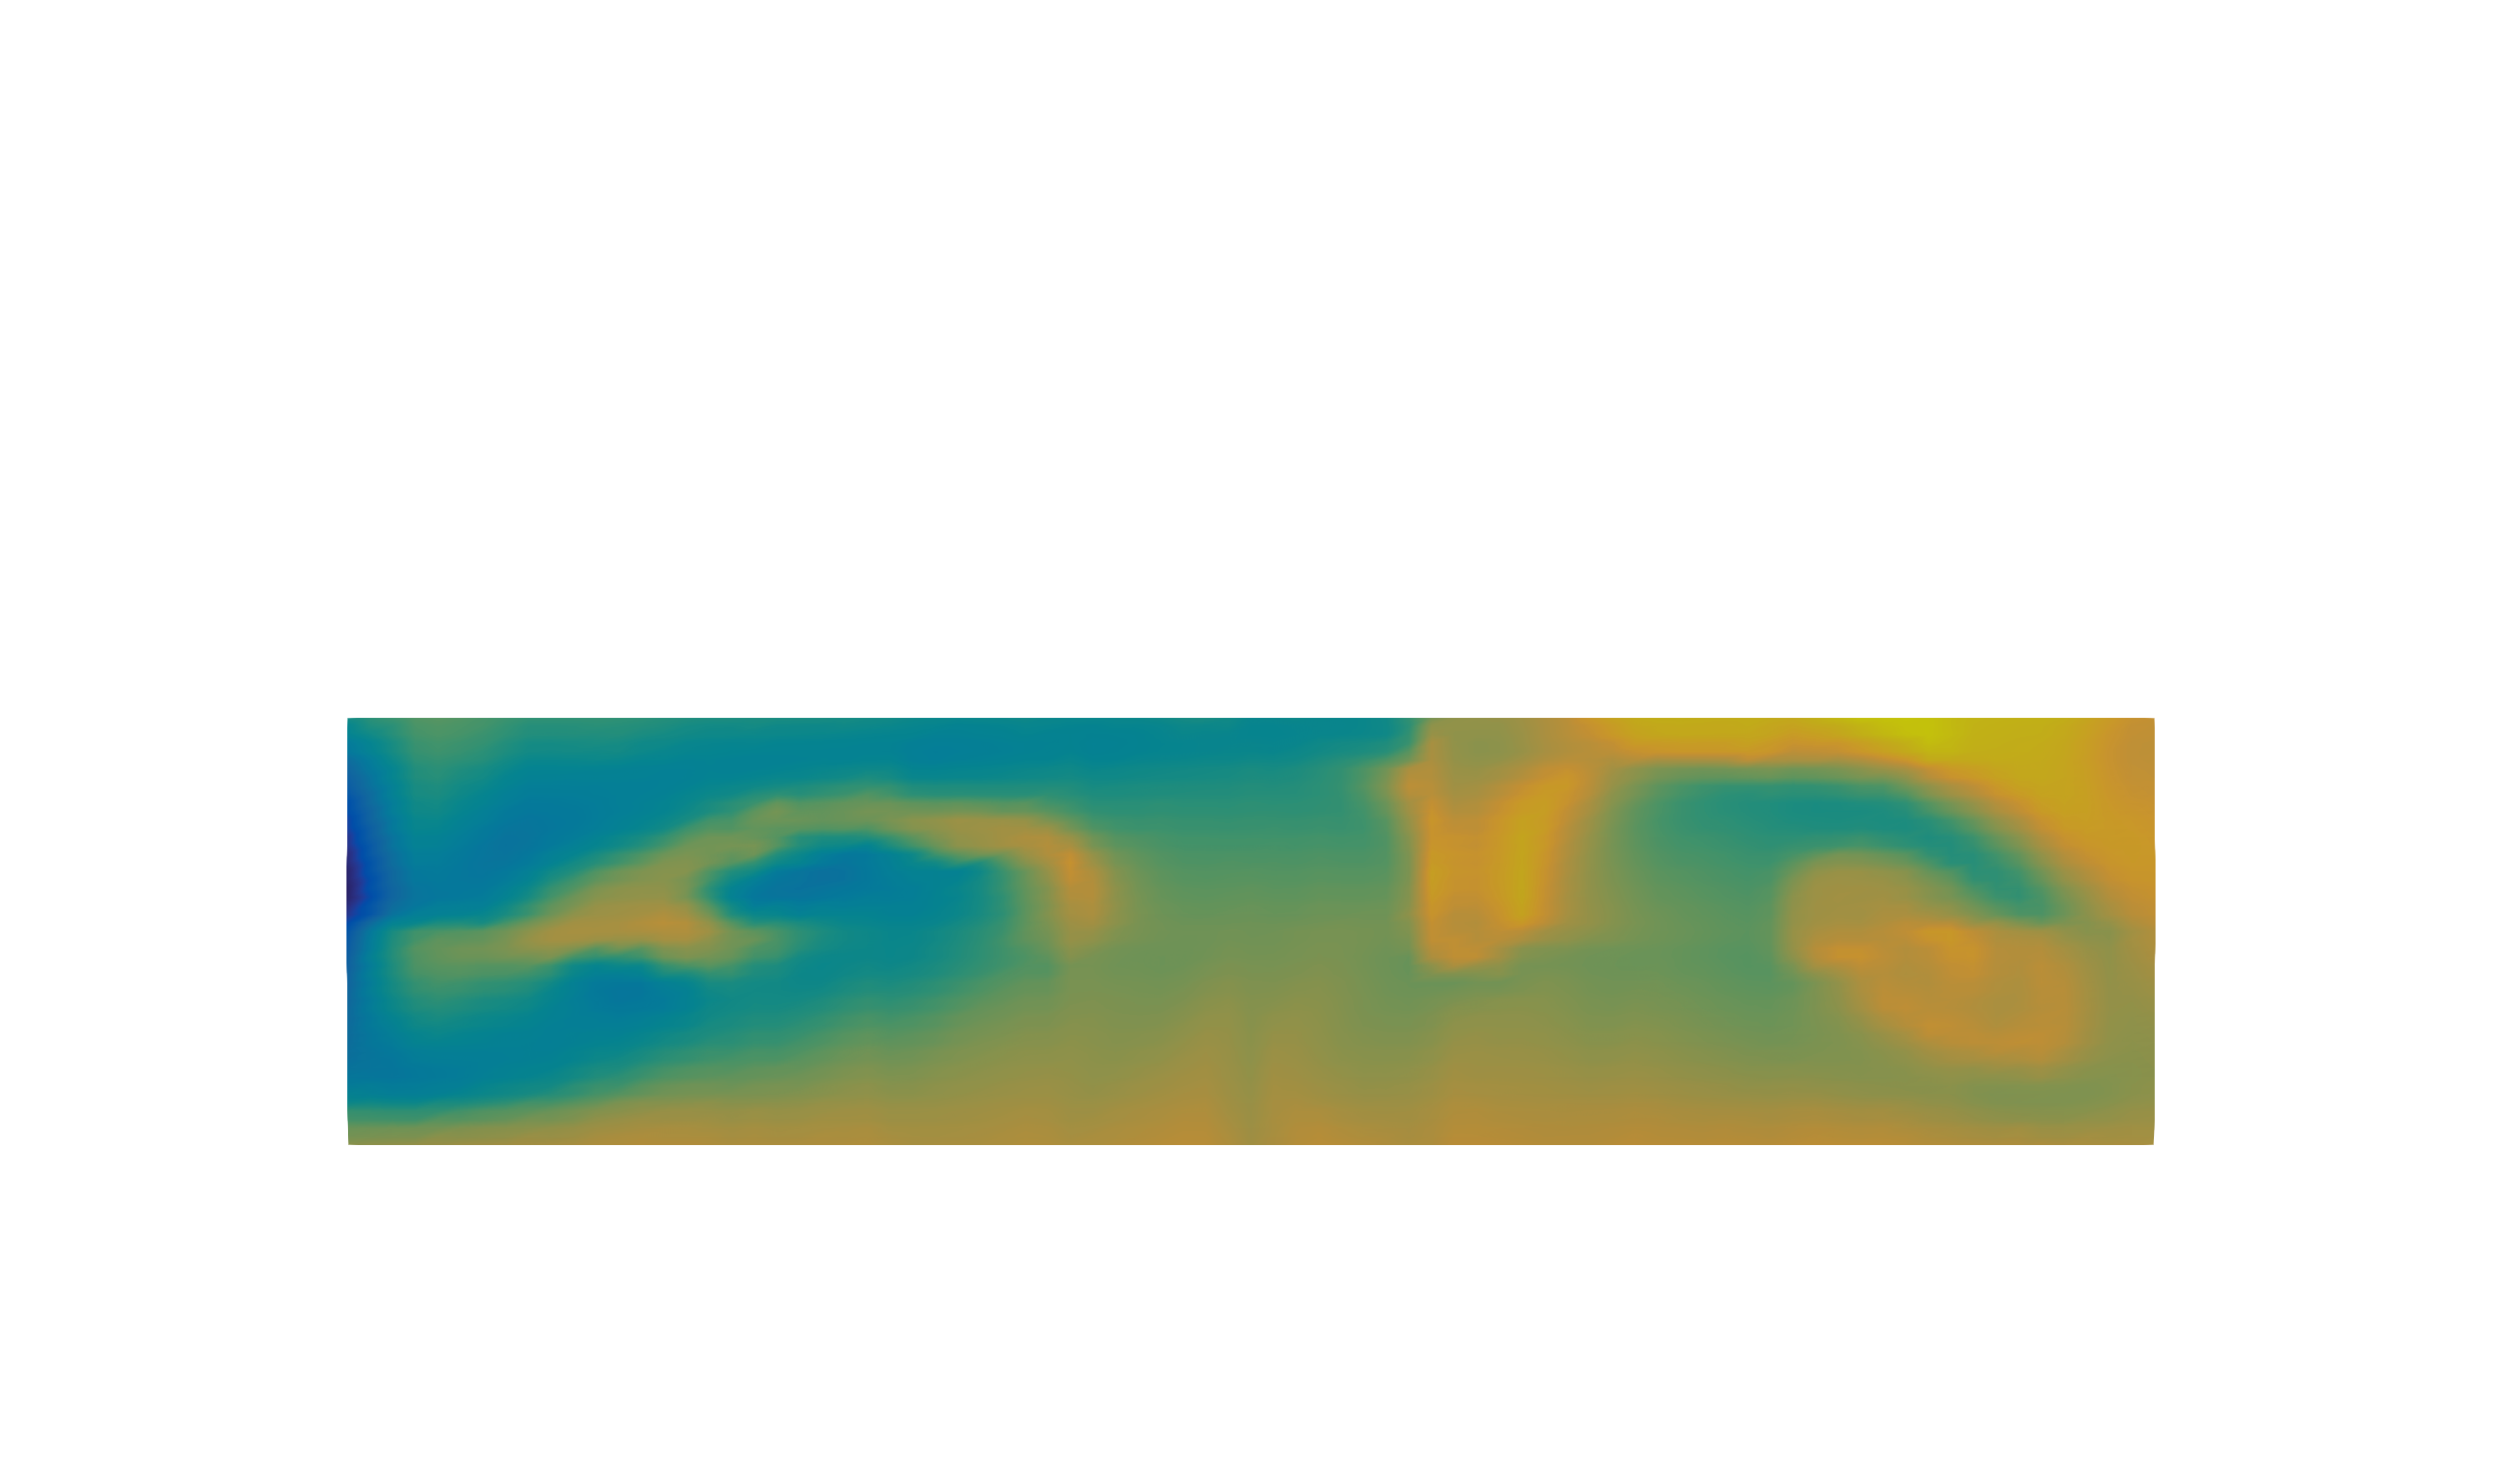
\includegraphics[width=\rasterimagewidth]{{../media/populations/application/print/alumina-influance-th1-2.54-3.08}.png}}};
        \end{axis}
      \end{tikzpicture}
      \begin{tikzpicture}
        \begin{axis}[
            %colorbar,
            hide axis,
            scale only axis,
            height=0.26\rasterimagewidth,,
            width=\rasterimagewidth,
            %colorbar horizontal,
            point meta min=2.54,
            point meta max=3.09,
            colorbar style={
              title=Concentration [\%w],
              width=7.4cm,
              height=0.3cm,
              xtick={2.54,2.75, 3,3.09, 3.5, 4, 4.5, 5, 5.5, 6},
              at={(0.5\rasterimagewidth,0.4cm)},
              anchor=north
            }
          ]
          \addplot [] coordinates {(0,0)};
          \node (myfirstpic) at (0,0) {\framebox{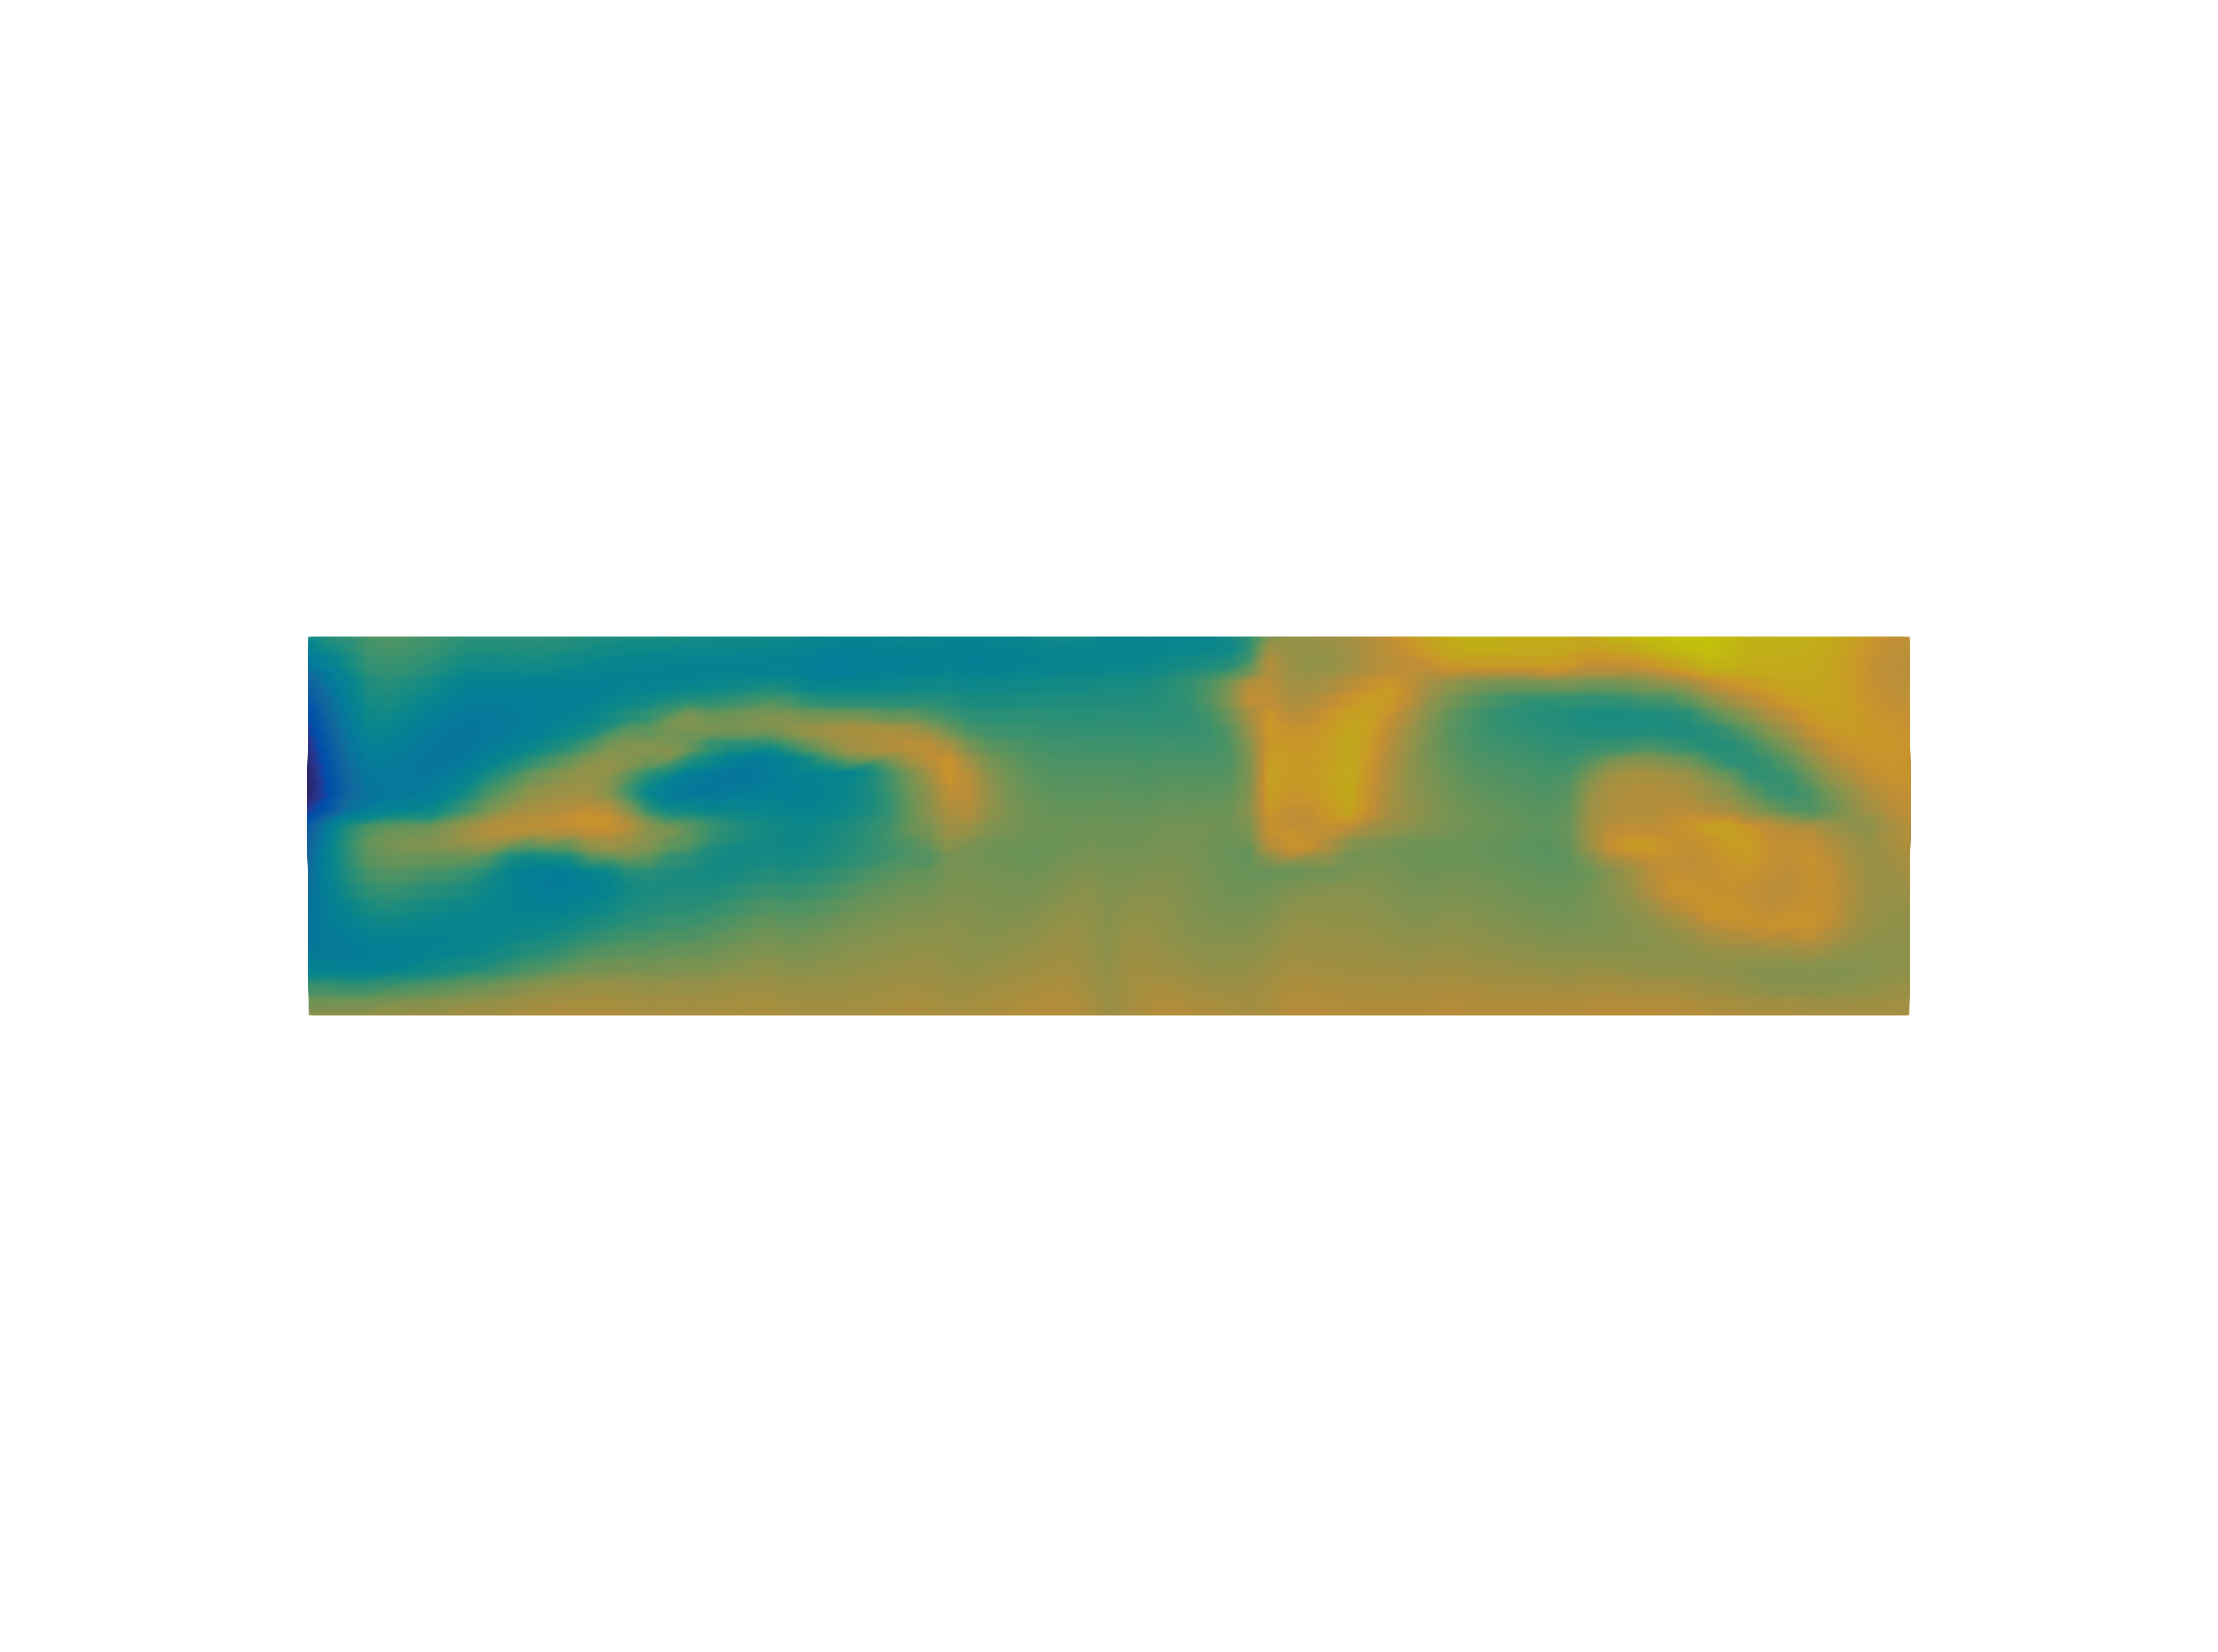
\includegraphics[width=\rasterimagewidth]{{../media/populations/application/print/alumina-influance-th2-2.54-3.09}.png}}};
        \end{axis}
      \end{tikzpicture}
      \begin{tikzpicture}
        \begin{axis}[
            %colorbar,
            hide axis,
            scale only axis,
            height=0.26\rasterimagewidth,,
            width=\rasterimagewidth,
            %colorbar horizontal,
            point meta min=2.54,
            point meta max=3.09,
            colorbar style={
              title=Concentration [\%w],
              width=7.4cm,
              height=0.3cm,
              xtick={2.54, 2.75, 3, 3.09, 3.5, 4, 4.5, 5, 5.5, 6},
              at={(0.5\rasterimagewidth,0.4cm)},
              anchor=north
            }
          ]
          \addplot [] coordinates {(0,0)};
          \node (myfirstpic) at (0,0) {\framebox{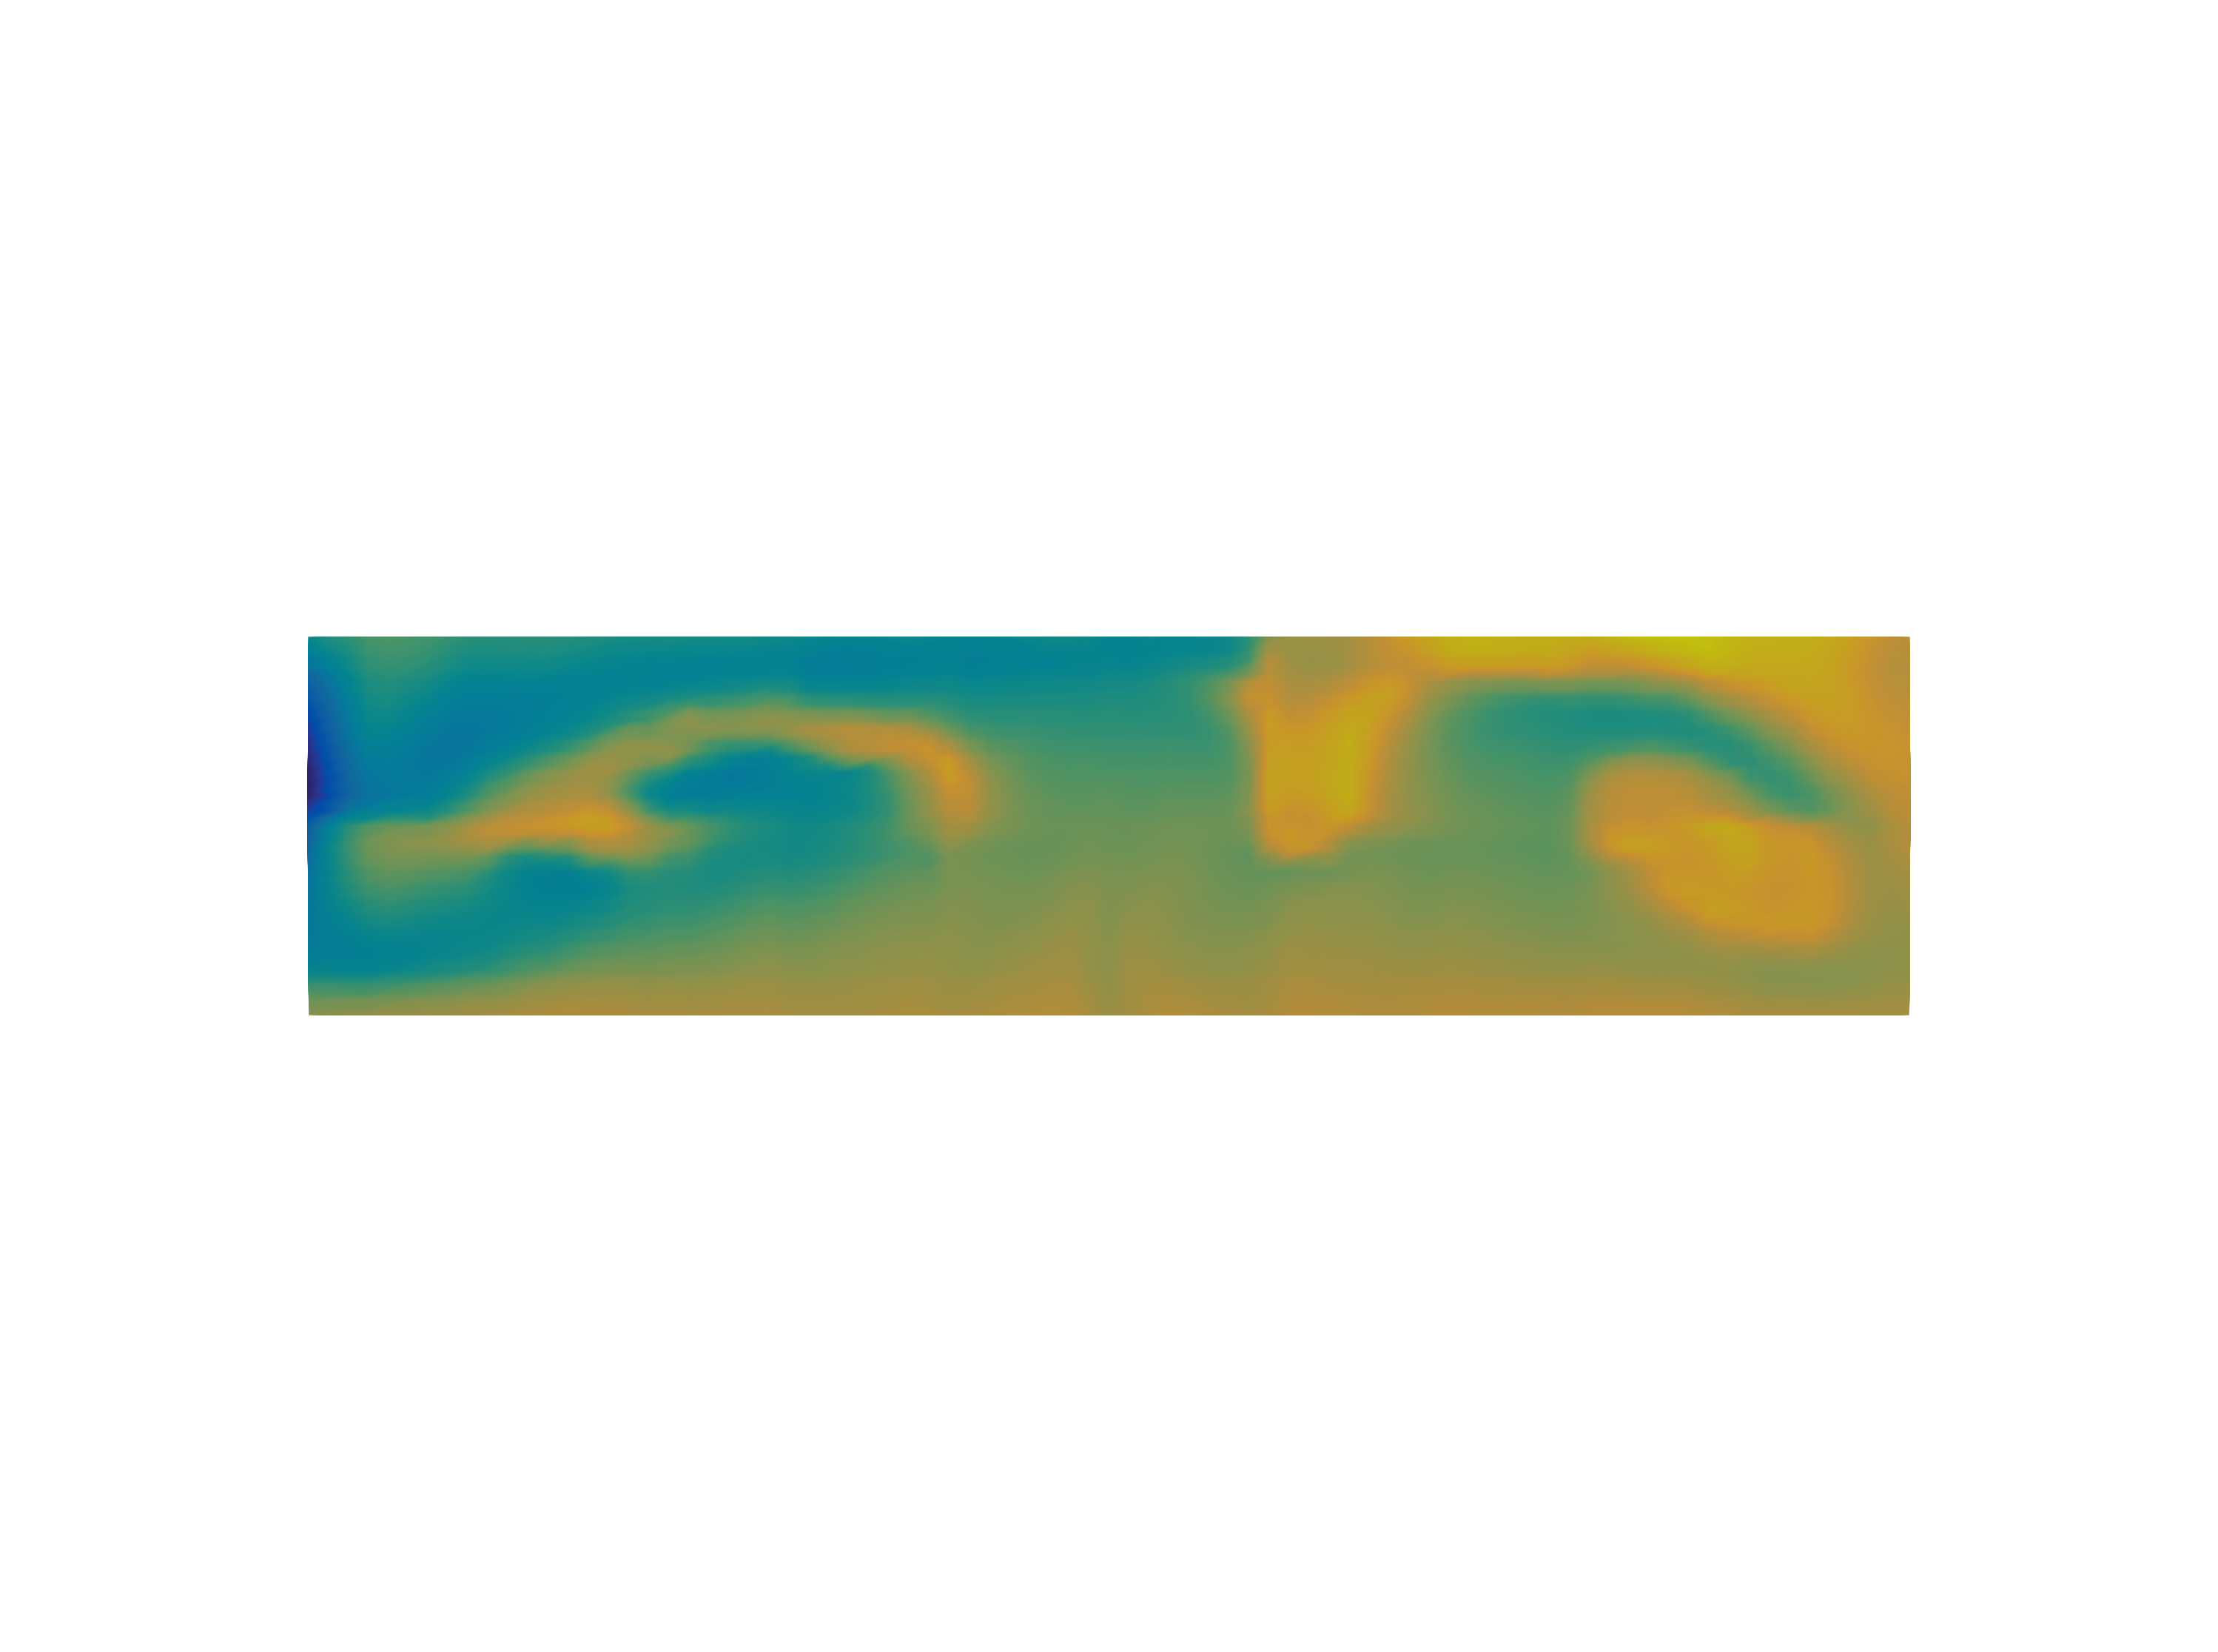
\includegraphics[width=\rasterimagewidth]{{../media/populations/application/print/alumina-influance-th5-2.54-3.09}.png}}};
        \end{axis}
      \end{tikzpicture}
      \begin{tikzpicture}
        \begin{axis}[
            colorbar,
            hide axis,
            scale only axis,
            height=0.52\rasterimagewidth,,
            width=\rasterimagewidth,
            colorbar horizontal,
            point meta min=2.54,
            point meta max=3.09,
            colorbar style={
              title=Concentration [\%w],
              width=7.4cm,
              height=0.3cm,
              xtick={2.54,2.75, 3, 3.09, 3.5, 4, 4.5, 5, 5.5, 6},
              at={(0.5\rasterimagewidth,3.0cm)},
              anchor=north
            }
          ]
          \addplot [] coordinates {(0,0)};
          \node (myfirstpic) at (0,50) {{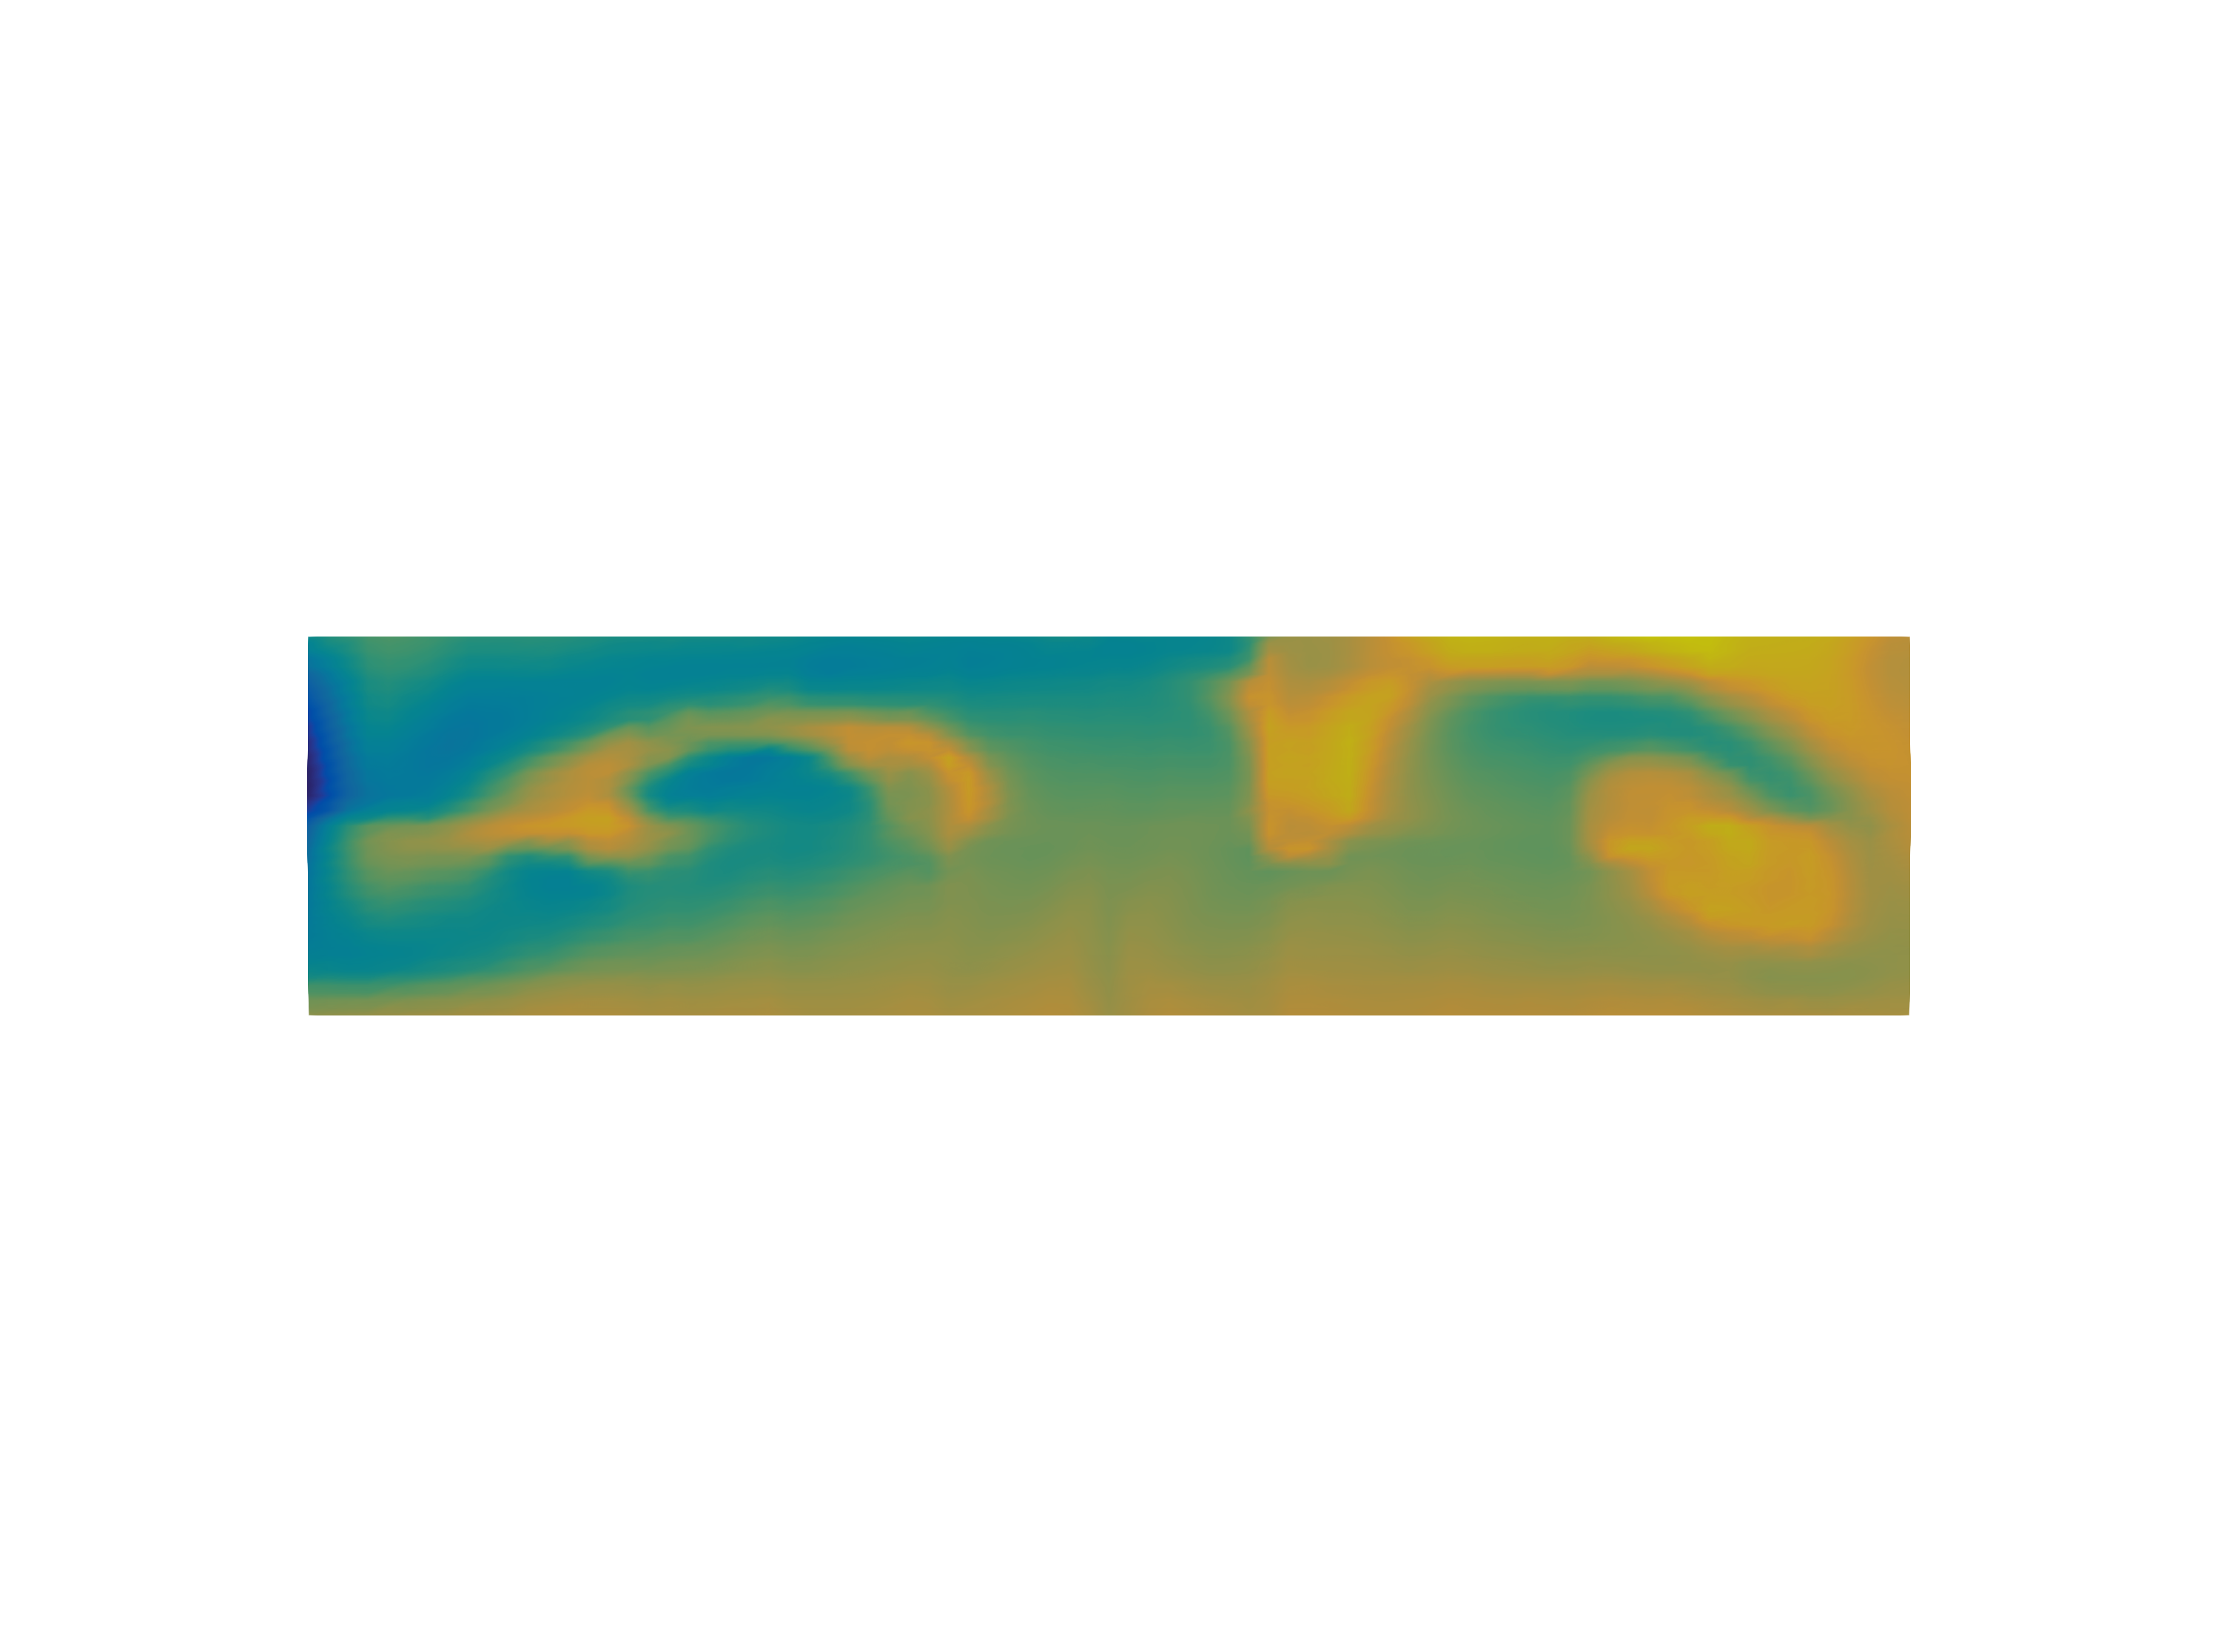
\includegraphics[width=\rasterimagewidth]{{../media/populations/application/print/alumina-influance-th510-2.54-3.09}.png}}};
        \end{axis}
      \end{tikzpicture}
    \caption{Champ de concentration $c$ dans l'ACD de la cuve AP32 à
      $t = \num{10000}$ \si{second}. De haut en bas, le temps de
      latence de dissolution $T_\text{Lat} = 1\si\second$,
      $2\si\second$, $5\si\second$ et $10\si\second$.}
    \label{fig:dissolution-alumin-influence-tlat}
  \end{center}
\end{figure}


La figure \ref{fig:dissolution-alumin-influence-tlat} présente la
distribution de concentration d'alumine dissoute dans l'ACD de la cuve
AP32 à $T = $ \num{10000} \si{\second} pour les différentes valeurs
de $\tlat$ croissantes de haut en bas.

Les quatre champs de concentration présentés sur la figure
\ref{fig:dissolution-alumin-influence-tlat} sont très similaires. Les
maxima et les minima de la concentration d'alumine
sont les mêmes et apparaissent aux mêmes endroits. On remarque
malgré tout de petites modifications de la distribution d'alumine
dissoute au voisinage des points d'injection. On observe par exemple
autour du point d'injection \#2 que la concentration est plus diffuse
lorsque $\tlat$ croît.

Nous nous intéressons maintenant à l'effet de la température
initiale du bain sur la distribution de la concentration d'alumine dissoute.

% Sensibilité par rapport a la surchauffe du bain
\paragraph{Sensibilité par rapport à la surchauffe initiale du bain}
La vitesse de dissolution des particules dans l'électrolyte
(\ref{eq:dissolution-velocity}) dépend de la température locale de
celui-ci. Comme rendu explicite par l'expression
(\ref{eq:conductivity-condition}), sous l'hypothèse que chaque dose de
particules se dissout entièrement en un temps fini, le terme source
d'énergie par effet Joule est construit de sorte à maintenir une
quantité d'énergie thermique constante en moyenne dans le temps. En
l'absence de transition de phase dans l'électrolyte, cela signifie que
la température moyenne au cours du temps de celui-ci est maintenue
constante. Par conséquent, une température initiale du bain $\tinit$
plus élevée conduit à une température $\temperature$ dans l'état
périodique plus élevée en moyenne au cours d'une période
du cycle d'injection global.

\begin{figure}[!hp]
  \begin{center}
      \begin{tikzpicture}
        \begin{axis}[
            %colorbar,
            hide axis,
            scale only axis,
            height=0.41\rasterimagewidth,,
            width=\rasterimagewidth,
            %colorbar horizontal,
            point meta min=2.43,
            point meta max=3.05,
            colorbar style={
              title=Concentration [\%w],
              width=7.4cm,
              height=0.3cm,
              xtick={2.43,2.5,2.75, 3, 3.05, 3.5, 4, 4.5, 5, 5.5, 6},
              at={(0.5\rasterimagewidth,0.4cm)},
              anchor=north
            }
          ]
          \addplot [] coordinates {(0,0)};
          \node (myfirstpic) at (0,0) {\framebox{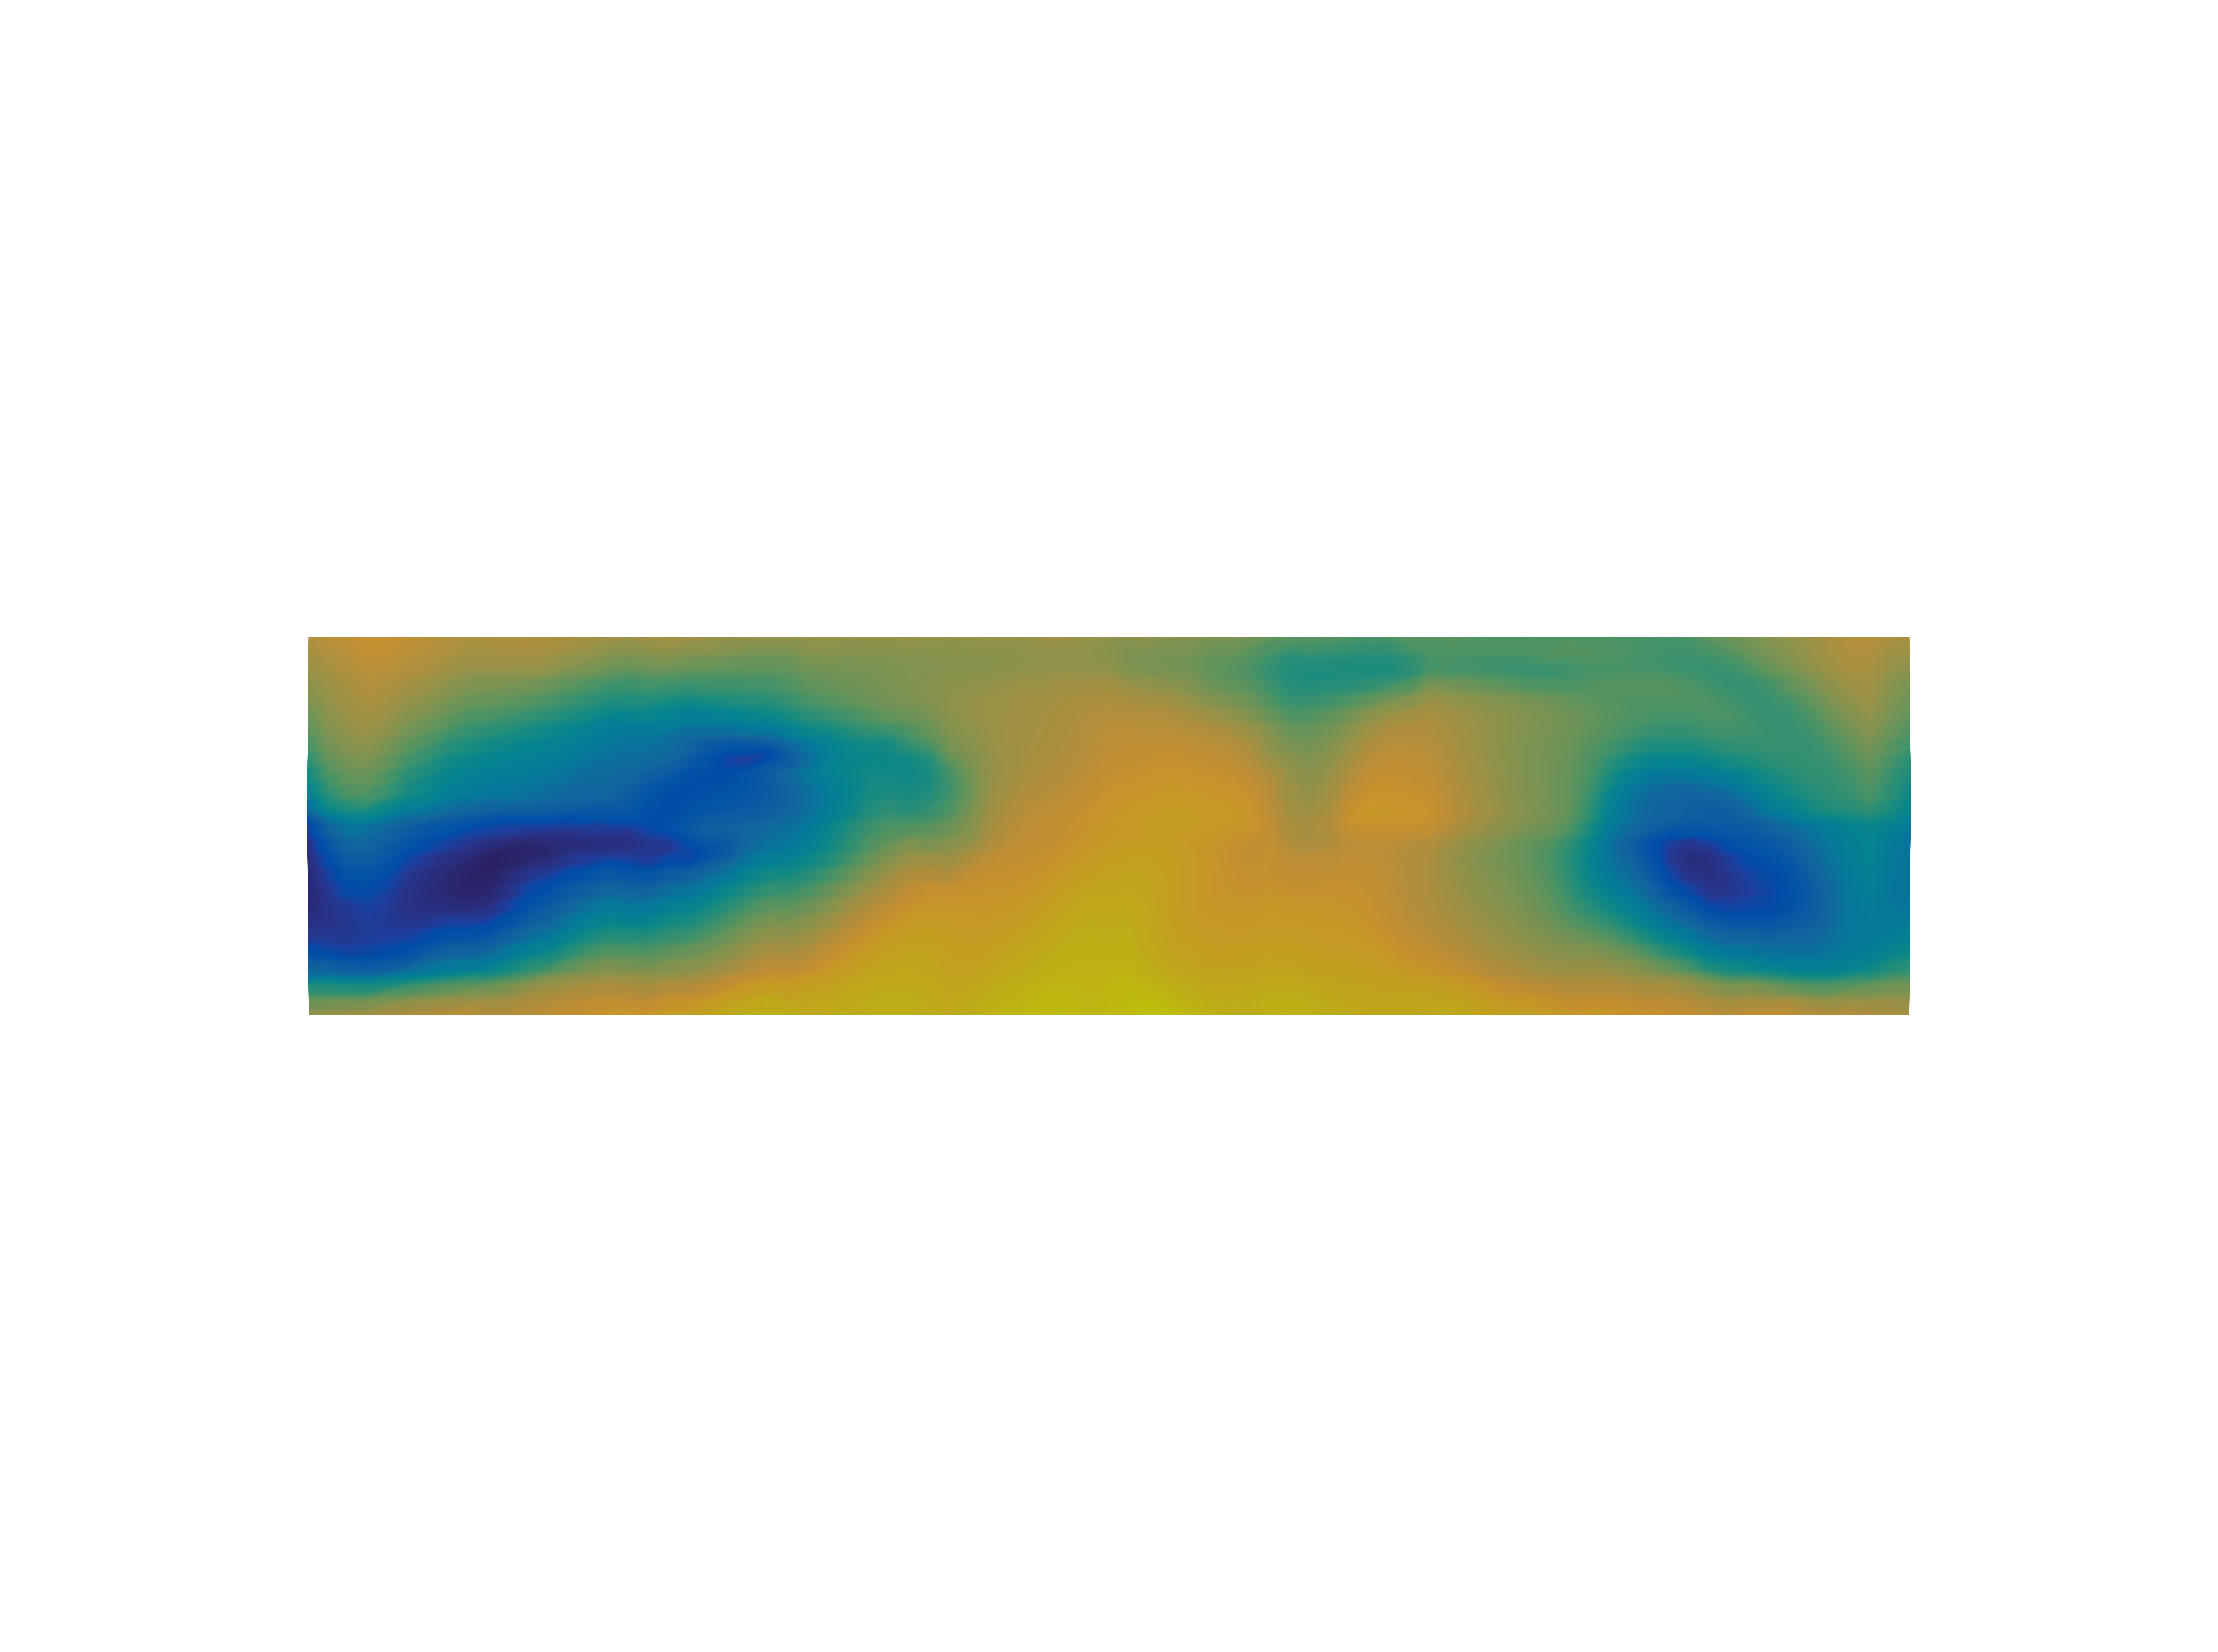
\includegraphics[width=\rasterimagewidth]{{../media/populations/application/print/alumina-influance-sur1-2.43-3.05}.png}}};
        \end{axis}
      \end{tikzpicture}
      \begin{tikzpicture}
        \begin{axis}[
            %colorbar,
            hide axis,
            scale only axis,
            height=0.41\rasterimagewidth,,
            width=\rasterimagewidth,
            %colorbar horizontal,
            point meta min=2.51,
            point meta max=3.02,
            colorbar style={
              title=Concentration [\%w],
              width=7.4cm,
              height=0.3cm,
              xtick={2.51,2.75, 3,3.02, 3.5, 4, 4.5, 5, 5.5, 6},
              at={(0.5\rasterimagewidth,0.4cm)},
              anchor=north
            }
          ]
          \addplot [] coordinates {(0,0)};
          \node (myfirstpic) at (0,0) {\framebox{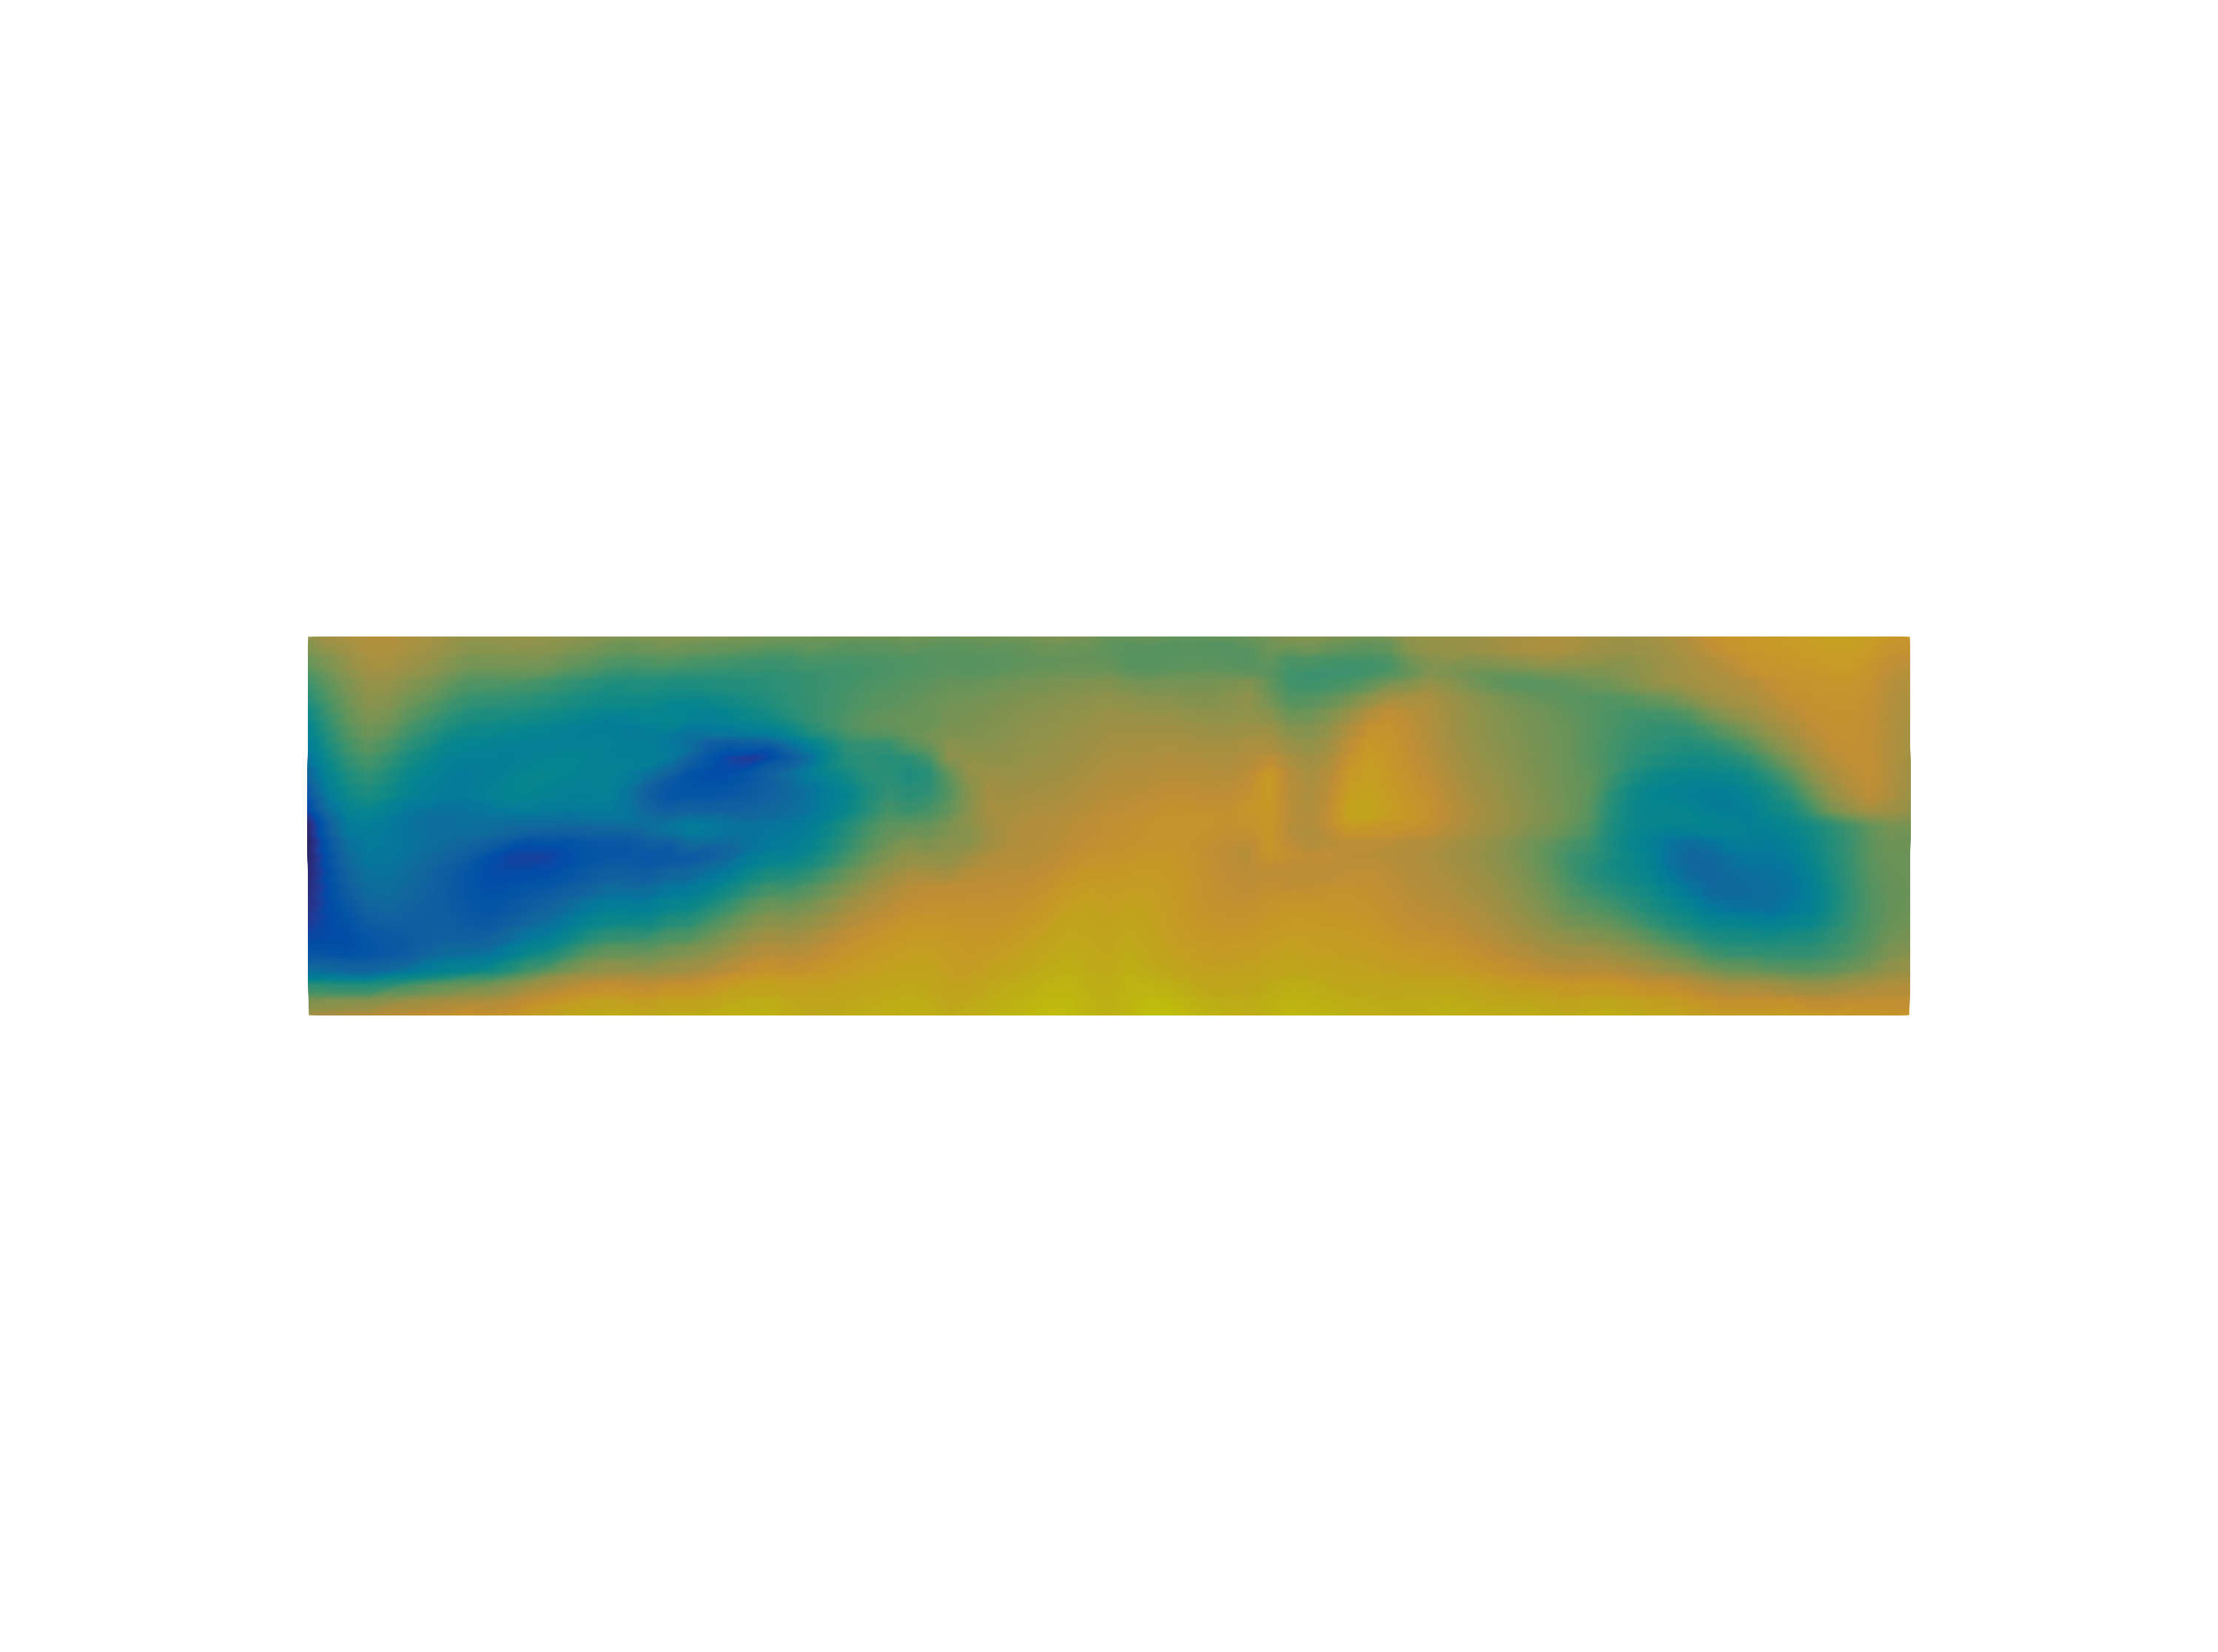
\includegraphics[width=\rasterimagewidth]{{../media/populations/application/print/alumina-influance-sur2-2.51-3.02}.png}}};
        \end{axis}
      \end{tikzpicture}
      \begin{tikzpicture}
        \begin{axis}[
            %colorbar,
            hide axis,
            scale only axis,
            height=0.41\rasterimagewidth,,
            width=\rasterimagewidth,
            %colorbar horizontal,
            point meta min=2.51,
            point meta max=3.13,
            colorbar style={
              title=Concentration [\%w],
              width=7.4cm,
              height=0.3cm,
              xtick={2.51,2.75, 3,3.13, 3.5, 4, 4.5, 5, 5.5, 6},
              at={(0.5\rasterimagewidth,0.4cm)},
              anchor=north
            }
          ]
          \addplot [] coordinates {(0,0)};
          \node (myfirstpic) at (0,0) {\framebox{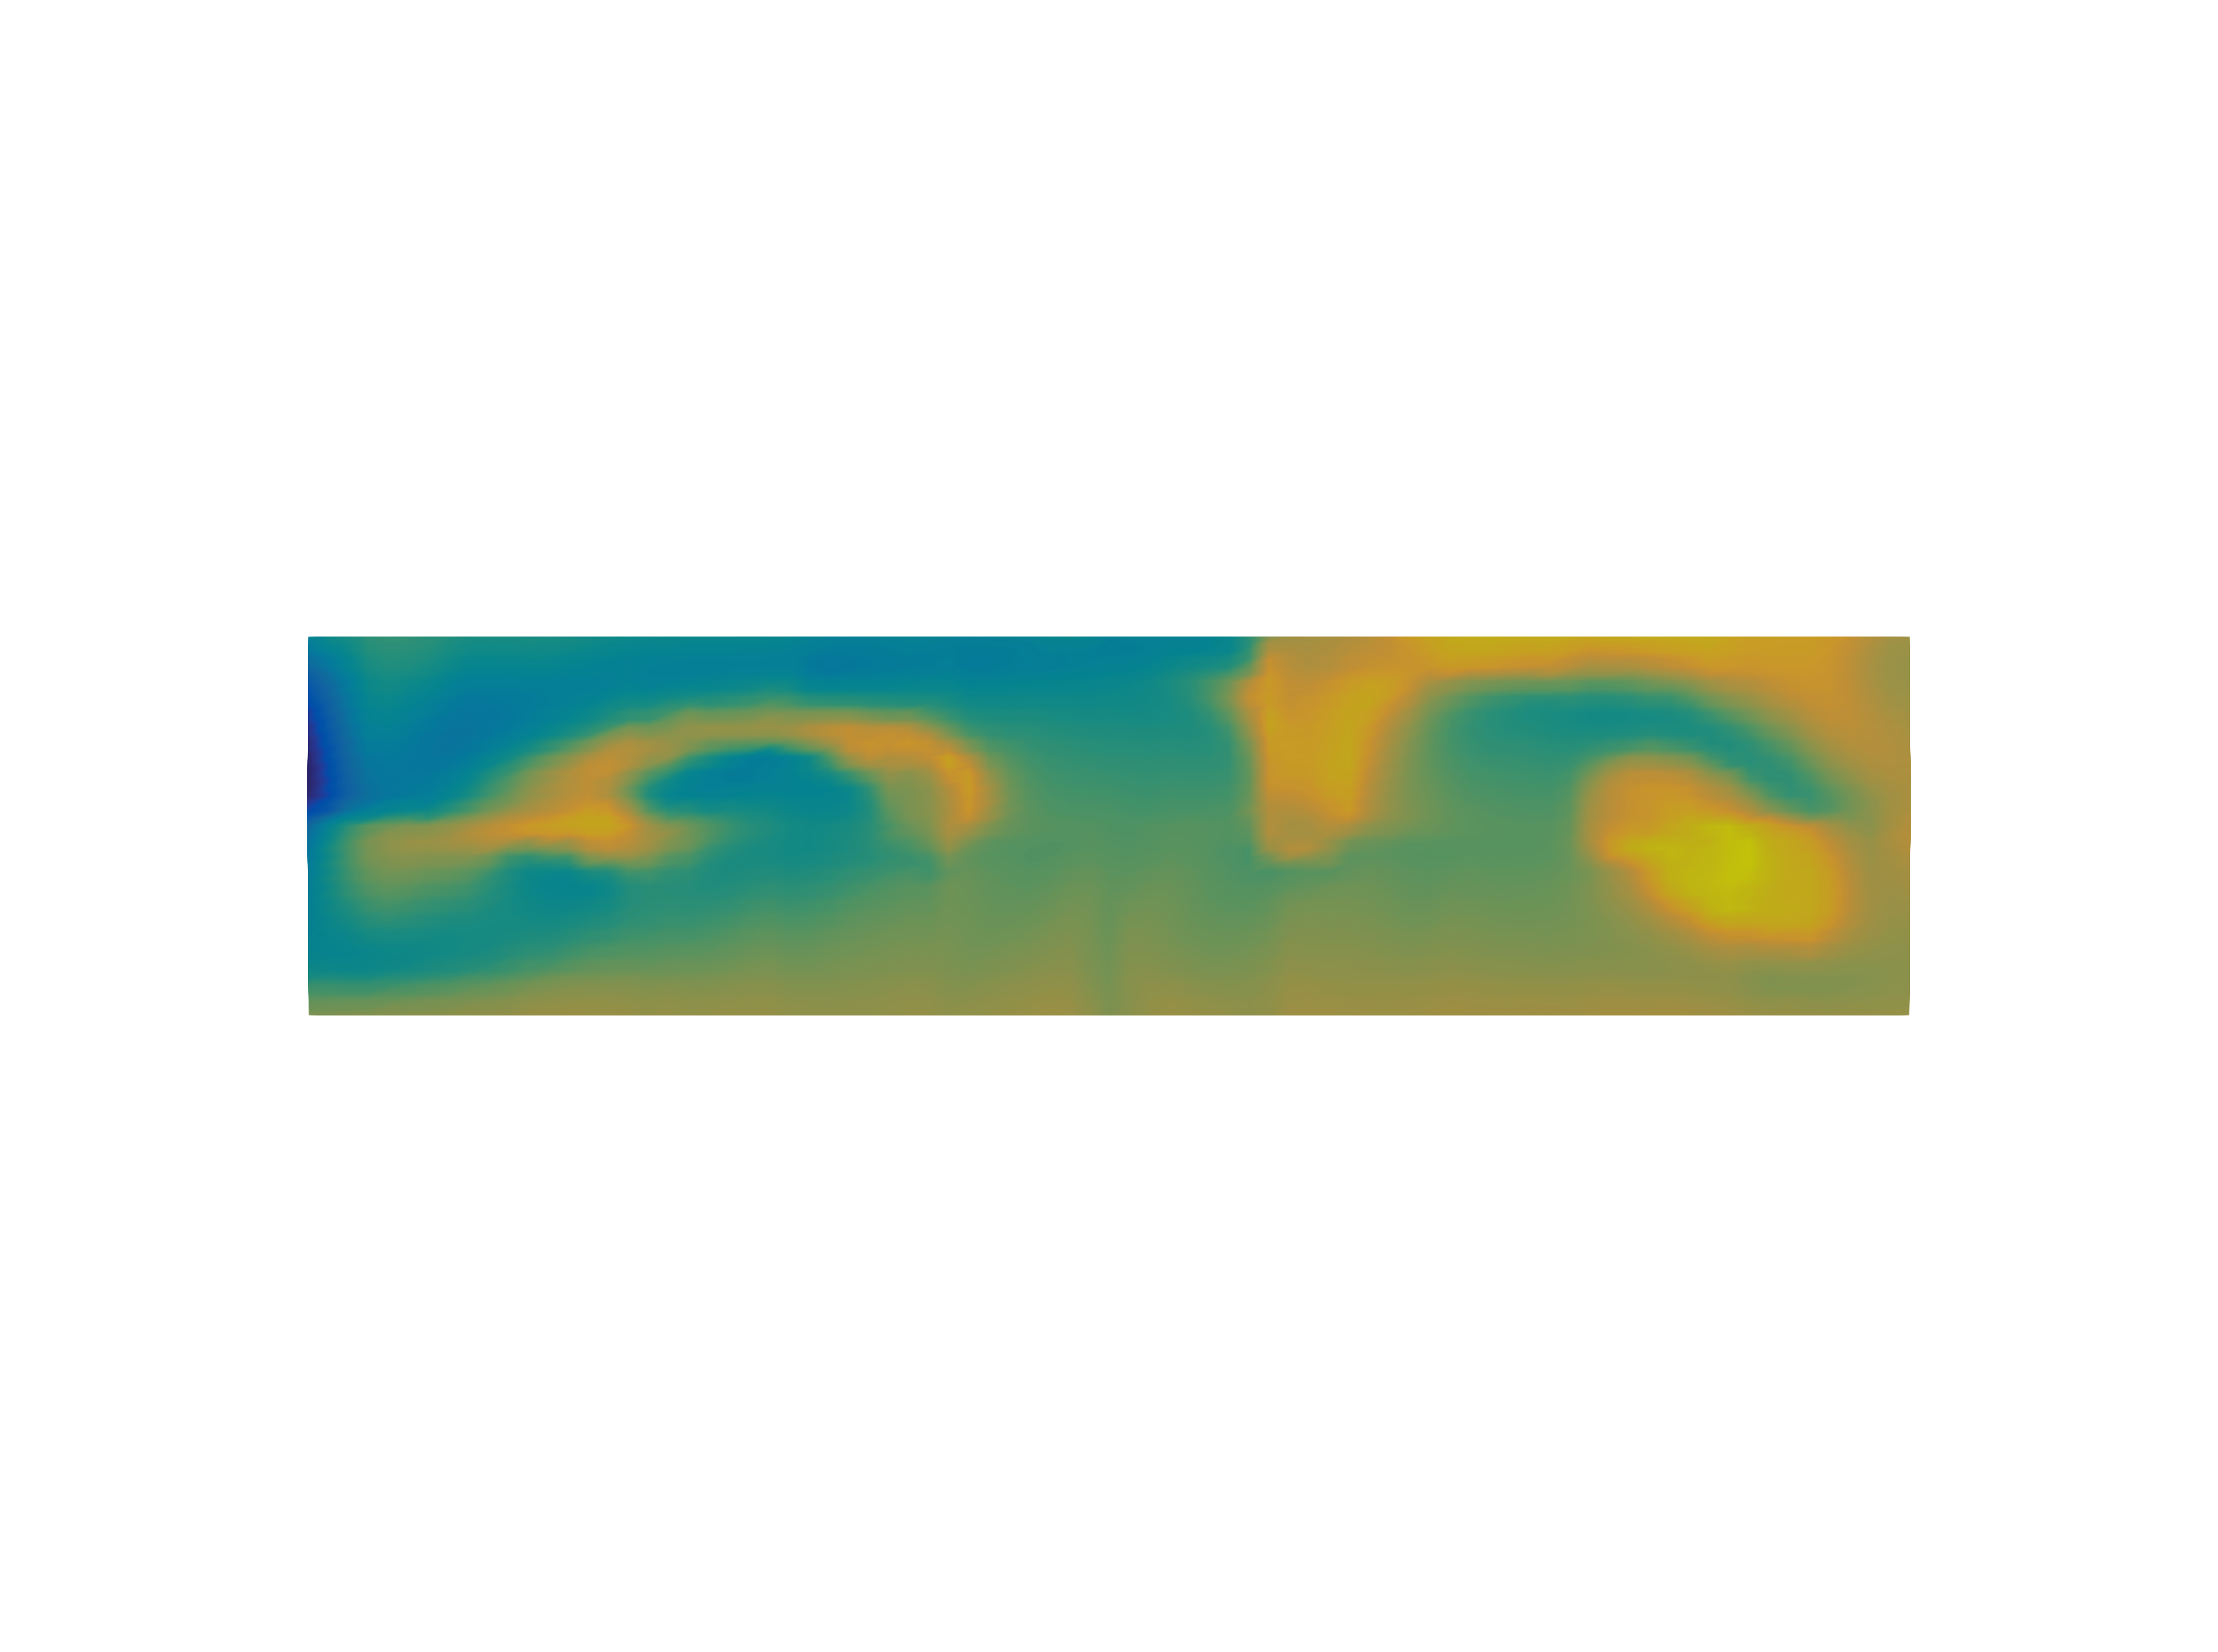
\includegraphics[width=\rasterimagewidth]{{../media/populations/application/print/alumina-influance-sur5-2.51-3.13}.png}}};
        \end{axis}
      \end{tikzpicture}
      \begin{tikzpicture}
        \begin{axis}[
            colorbar,
            hide axis,
            scale only axis,
            height=0.41\rasterimagewidth,,
            width=\rasterimagewidth,
            colorbar horizontal,
            point meta min=2.51,
            point meta max=3.13,
            colorbar style={
              title=Concentration [\%w],
              width=7.4cm,
              height=0.3cm,
              xtick={2.51, 2.75, 3, 3.13, 3.5, 4, 4.5, 5, 5.5, 6},
              at={(0.5\rasterimagewidth,0.4cm)},
              anchor=north
            }
          ]
          \addplot [] coordinates {(0,0)};
          \node (myfirstpic) at (0,0) {\framebox{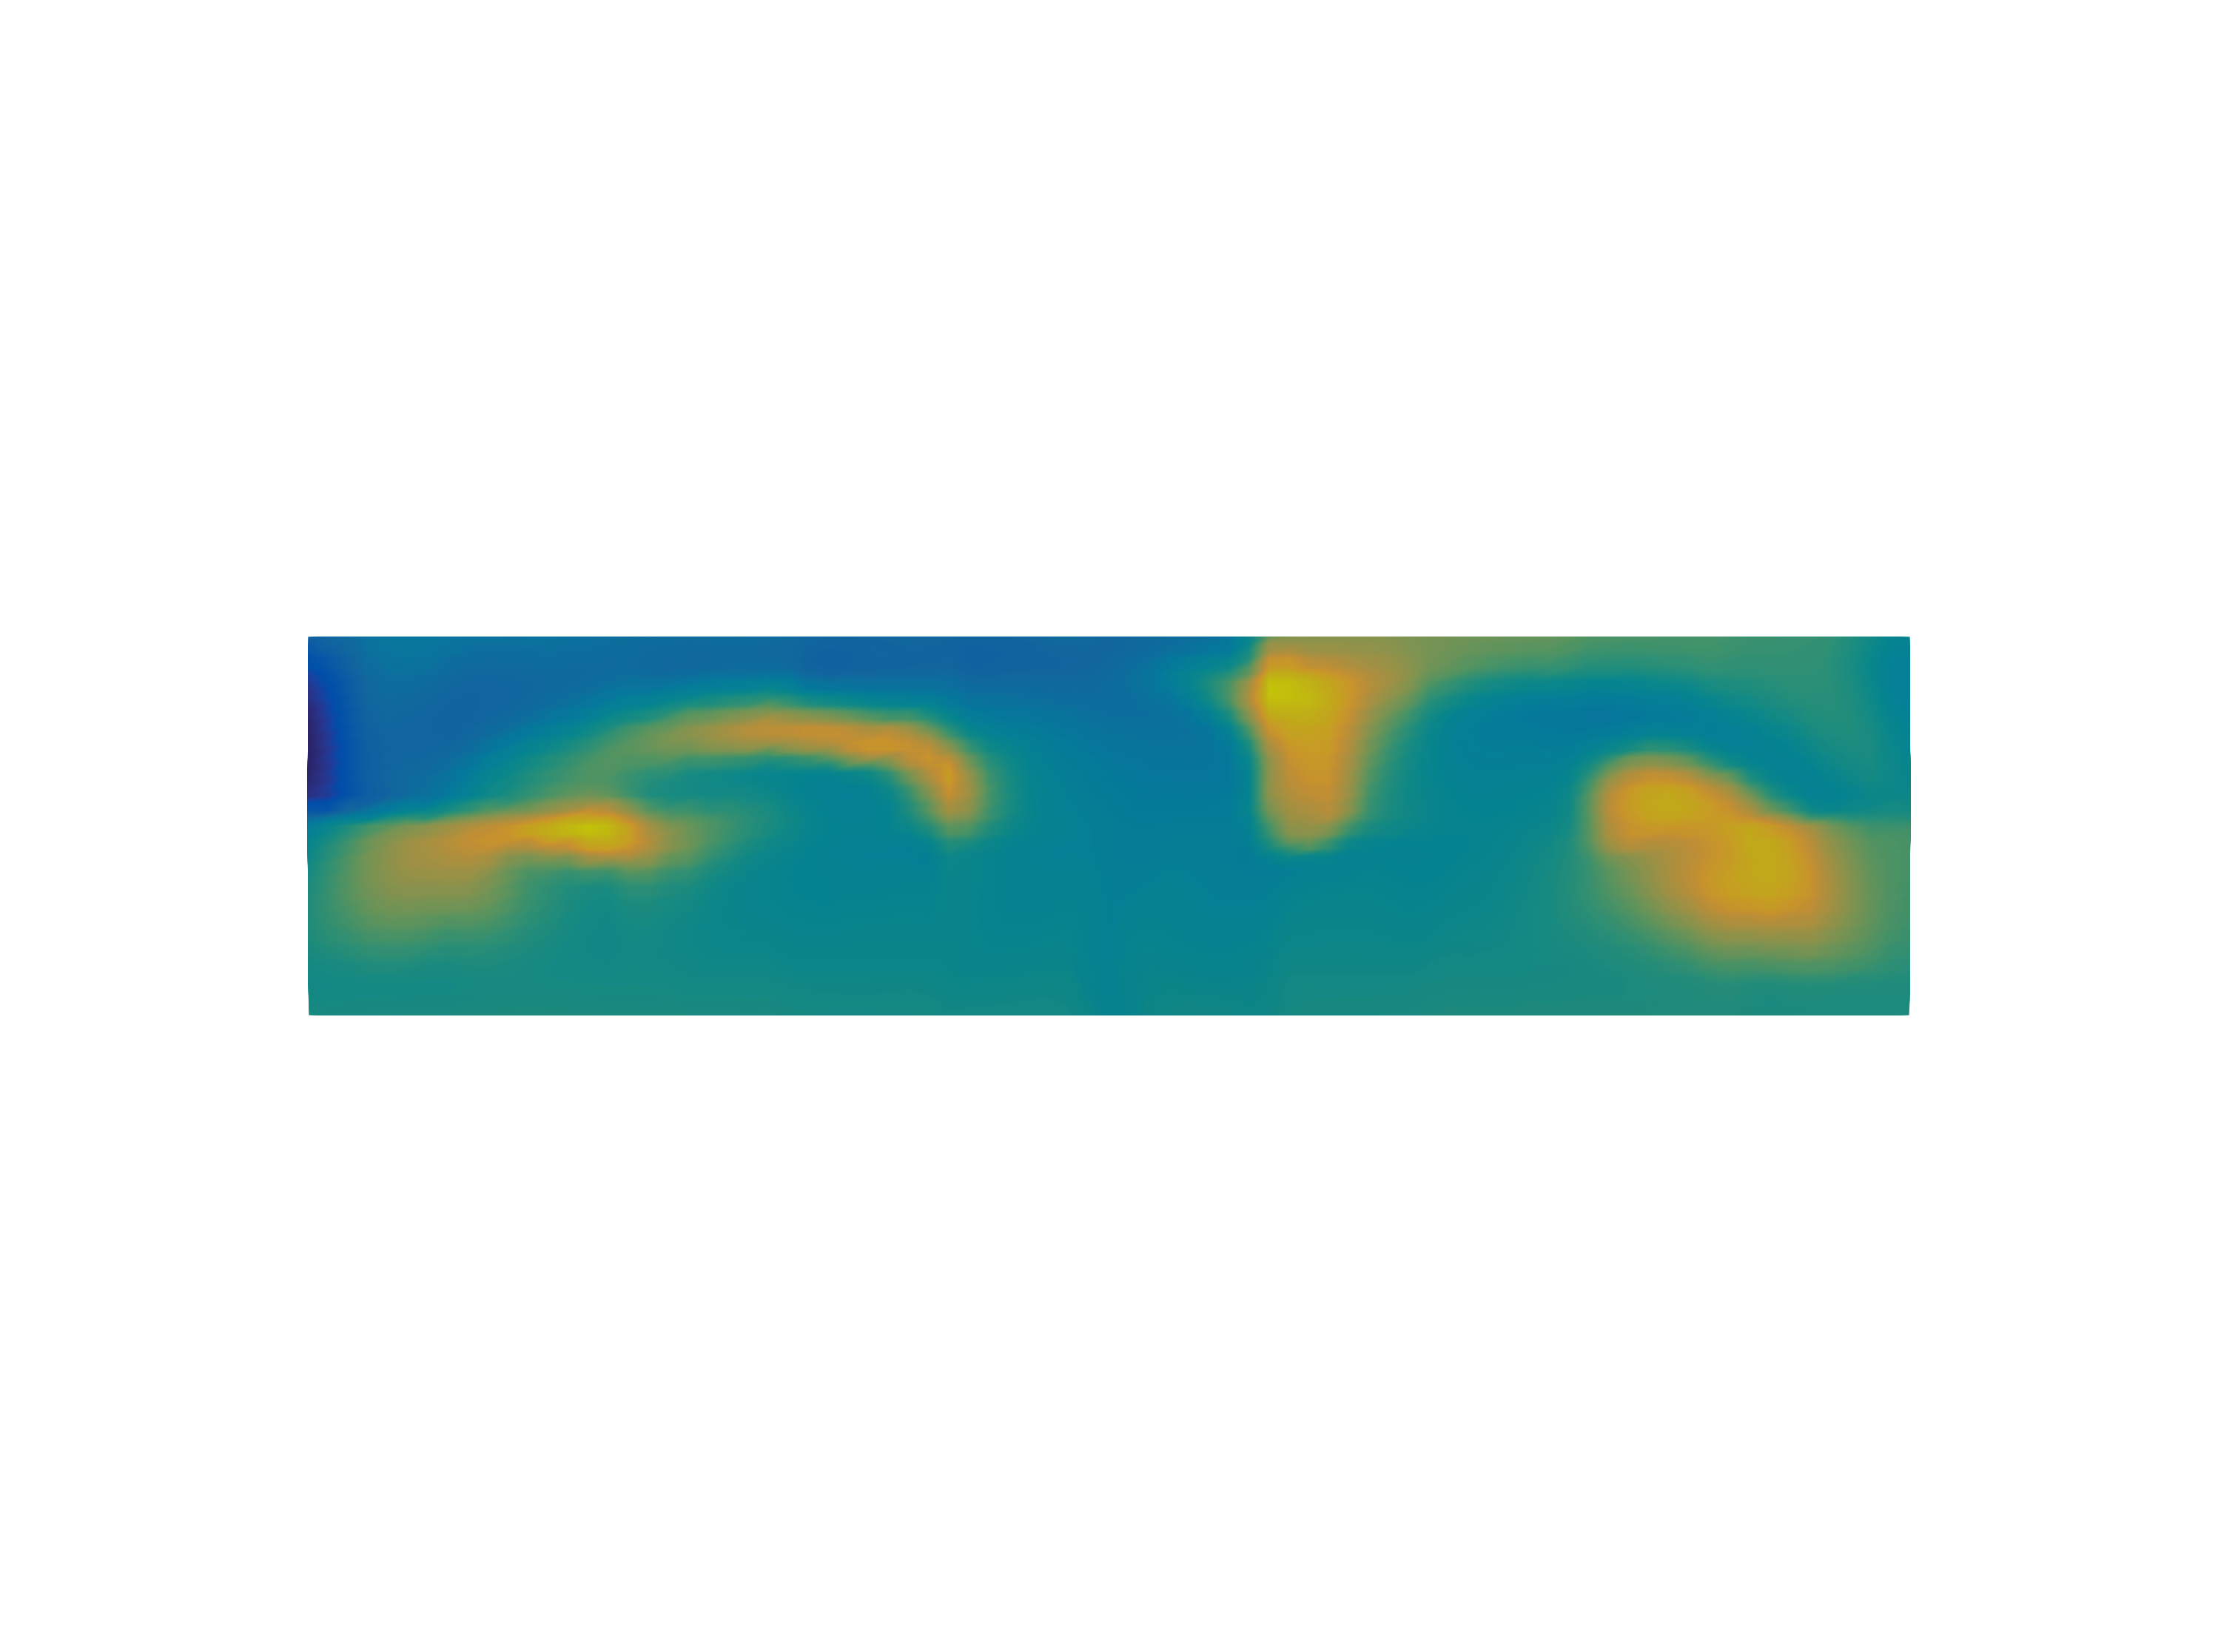
\includegraphics[width=\rasterimagewidth]{{../media/populations/application/print/alumina-influance-sur10-2.51-3.13}.png}}};
        \end{axis}
      \end{tikzpicture}
      \caption{Champ de concentration $c$ dans l'ACD de la cuve AP32 à
        $t = \num{10000}$ \si{\second}. De haut en bas, la température
        de surchauffe initiale est $\tsur = $ \numlist{1;2;5;10}.}
    \label{fig:dissolution-alumin-influence-sur}
  \end{center}
\end{figure}


Nous proposons d'évaluer la sensibilité de la dissolution d'alumine
dans le bain électrolytique en fonction de la température de celui-ci
en faisant varier la température initiale du bain. On note $\tsur$ la
température de surchauffe initiale du bain au-dessus de sa température de
liquidus:
\begin{equation}
  \tsur = \tinit - \tliq.
\end{equation}
La figure \ref{fig:dissolution-alumin-influence-sur} présente la distribution
de la concentration d'alumine dissoute $c$ dans l'ACD de la cuve AP32
issue de quatre calculs, pour lesquels les paramètres sont reportés
dans la table \ref{tab:dissolution-physical-parameters}, à
l'exception de la température initiale du bain $\tinit$. La
température initiale du bain est fixée à $\tinit = \tliq + \tsur$ avec
$\tsur = $ \numlist{1;2;5;10} degrés Kelvin.
\clearpage

Les champs de concentration sur la figure
\ref{fig:dissolution-alumin-influence-sur} correspondent de haut en
bas à des températures de surchauffe $\tsur$ croissante. On remarque
en particulier sur le dernier champ de concentration de cette figure,
qui correspond à $\tsur = $ \num{10} \si{\kelvin}, la similarité avec la
solution de référence illustrée sur la figure
\ref{fig:ap32-alumina-wo-t} pour laquelle la température ne joue pas
de rôle dans la dissolution des particules. Les valeurs maximales
atteintes par la concentration d'alumine dissoute sont cependant plus faibles.

Le premier champ de concentration de la figure
\ref{fig:dissolution-alumin-influence-sur} correspond à une
température de surchauffe $\tsur =$ \num{1} \si{\kelvin} et s'écarte
significativement de la solution de référence de la figure
\ref{fig:ap32-alumina-wo-t}. La concentration d'alumine dissoute est
homogène au point de ne plus pouvoir distinguer la position des
injecteurs.

La dissolution des particules d'alumine dépend d'une part du fait que
la température de l'électrolyte dans leur voisinage doit être
supérieure à la température du liquidus $\tliq$, et d'autre part de la
taille de la région de transition entre le régime de dissolution
contrôlé par la diffusion de l'énergie thermique et le régime de
dissolution contrôlé par la diffusion de l'alumine dissoute à
proximité de la surface des particules. La transition entre ces deux
régimes est contrôlée par le paramètre $\tcrit$. Dans le paragraphe
suivant nous proposons d'évaluer la distribution de concentration dans
le bain électrolytique en fonction du paramètre $\tcrit$.


% Sensibilité par rapport au modèle de dépendence (tcrit, exp vs heaviside)
\paragraph{Sensibilité par rapport à la température critique de transition}
\begin{figure}[!hp]
  \begin{center}
      \begin{tikzpicture}
        \begin{axis}[
            colorbar,
            hide axis,
            scale only axis,
            height=0.41\rasterimagewidth,
            width=\rasterimagewidth,
            colorbar horizontal,
            point meta min=2.55,
            point meta max=3.08,
            colorbar style={
              title=Concentration [\%w],
              width=7.4cm,
              height=0.3cm,
              xtick={2.5,2.55, 2.75, 3, 3.08, 3.5, 4, 4.5, 5, 5.5, 6},
              at={(0.5\rasterimagewidth,0.4cm)},
              anchor=north
            }
          ]
          \addplot [] coordinates {(0,0)};
          \node (myfirstpic) at (0,0) {\framebox{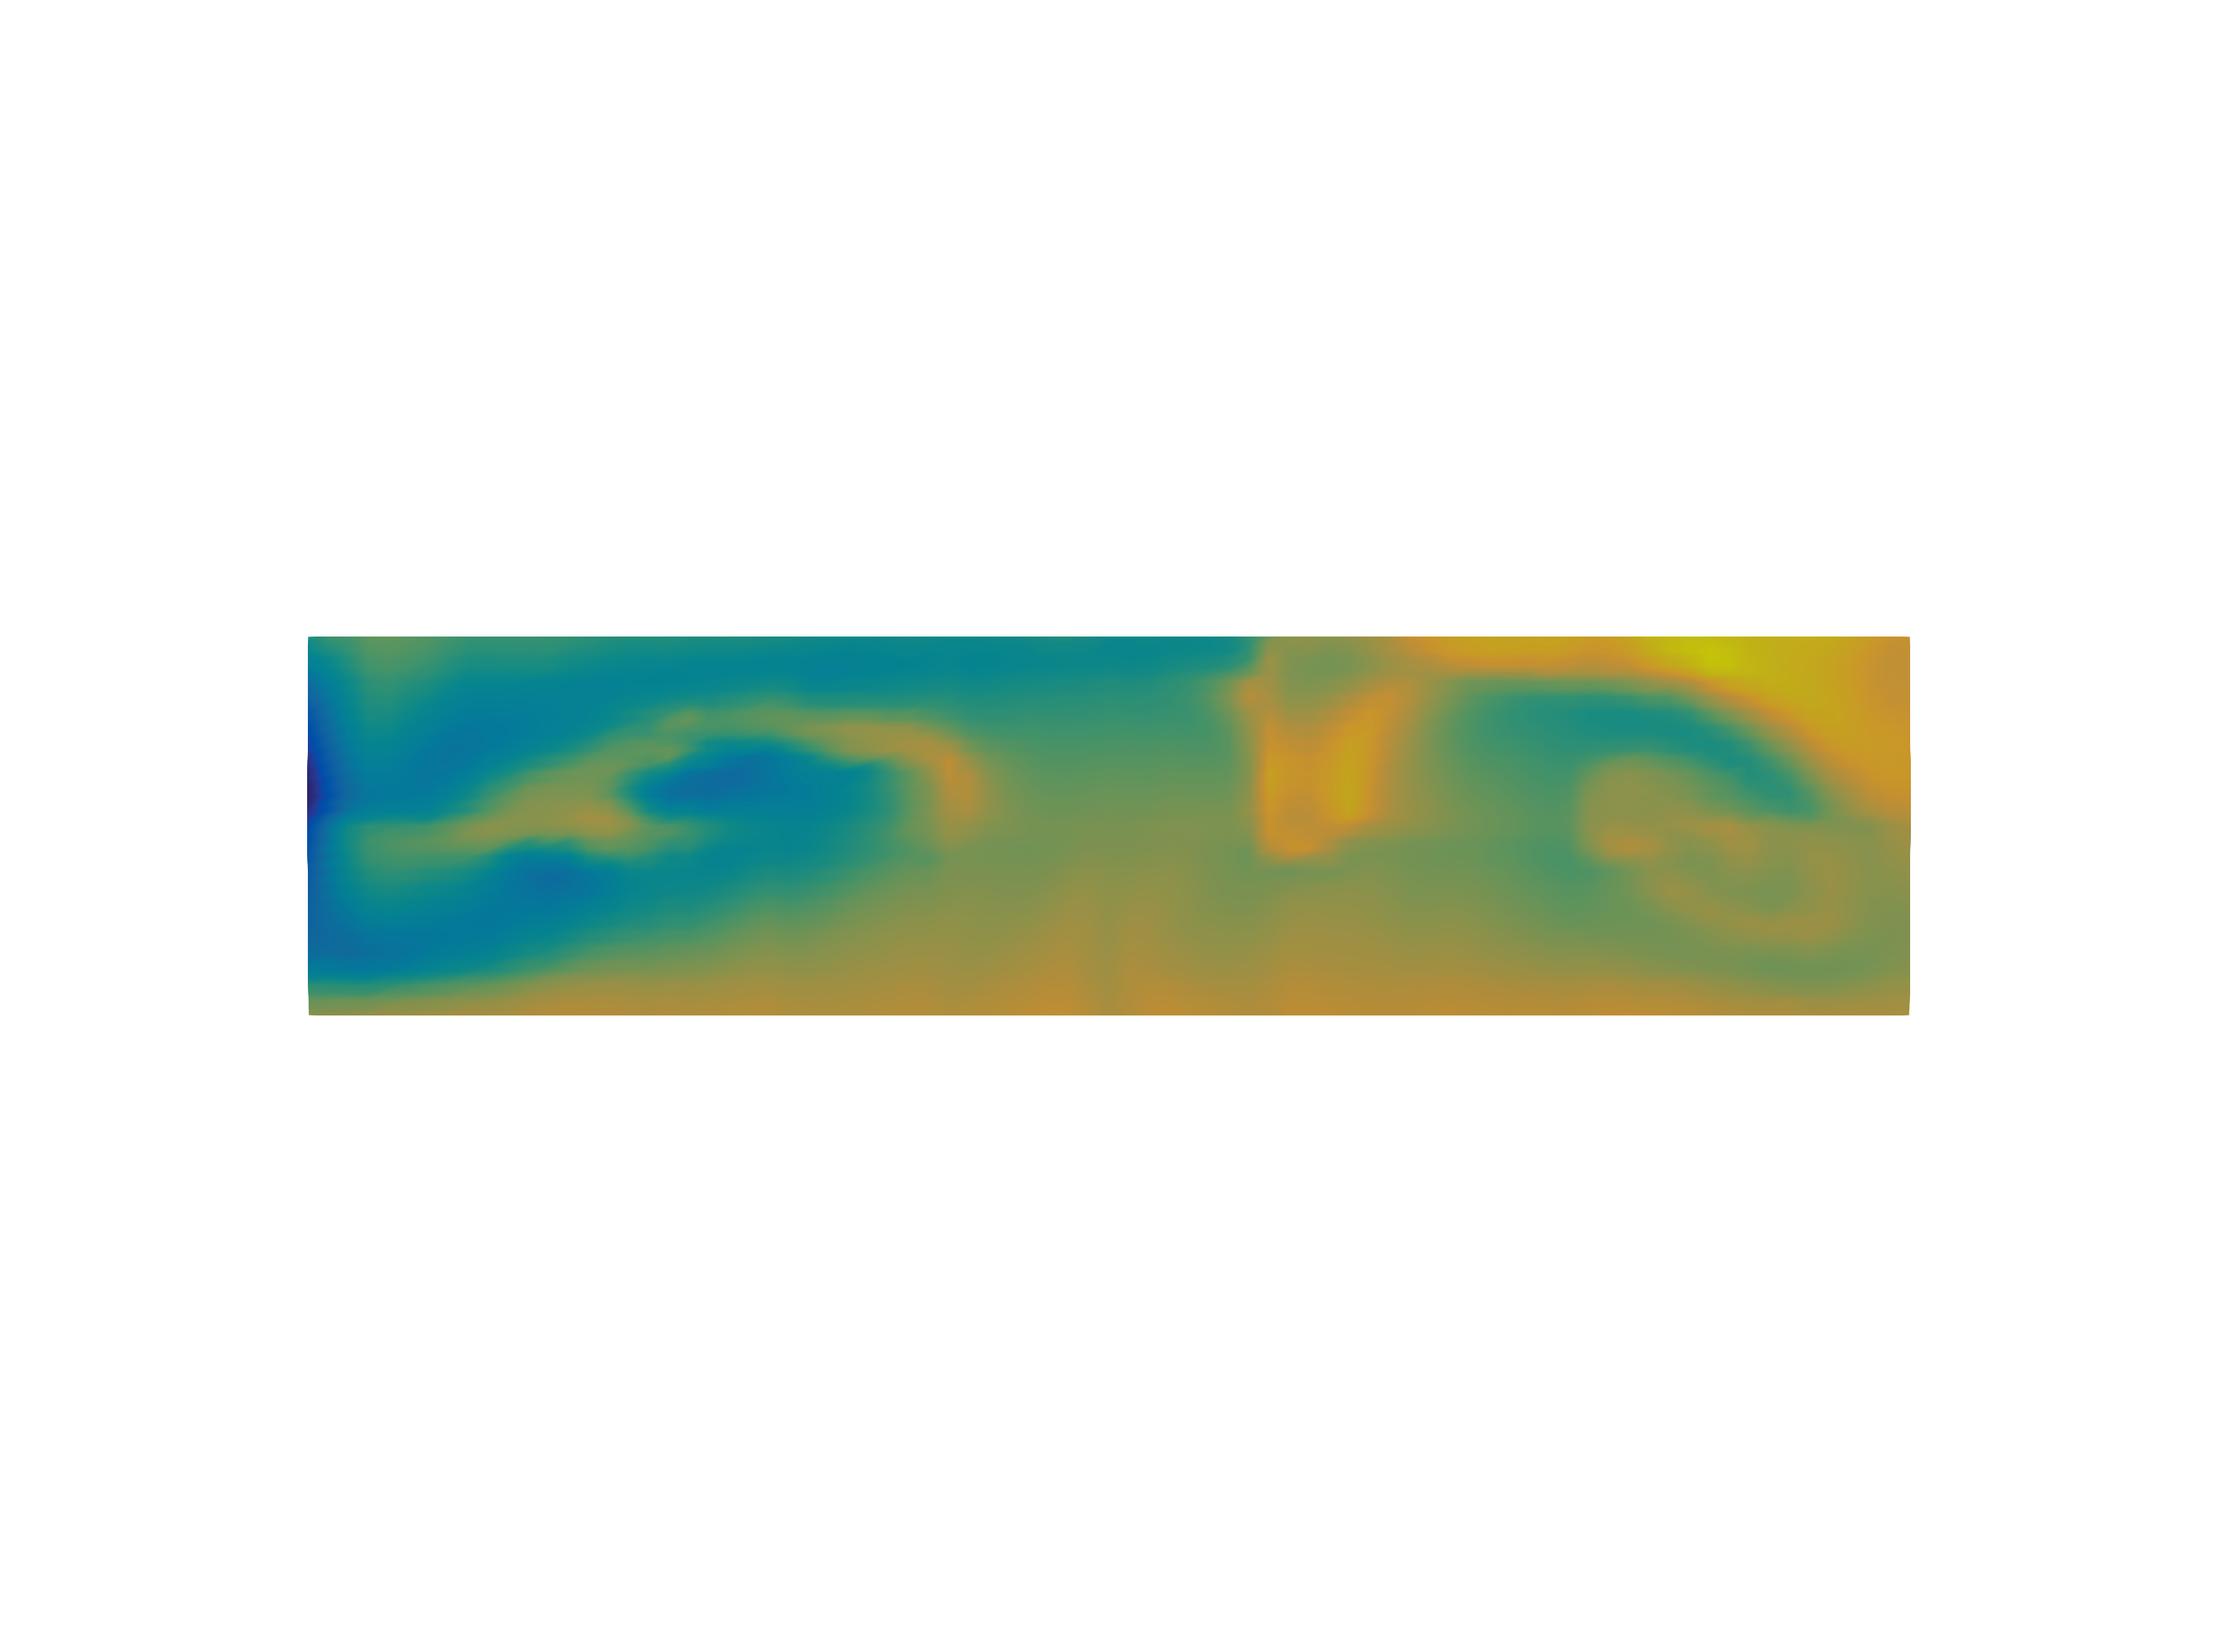
\includegraphics[width=\rasterimagewidth]{{../media/populations/application/print/alumina-influance-heaviside-2.55-3.08}.png}}};
        \end{axis}
      \end{tikzpicture}
      \begin{tikzpicture}
        \begin{axis}[
            colorbar,
            hide axis,
            scale only axis,
            height=0.41\rasterimagewidth,,
            width=\rasterimagewidth,
            colorbar horizontal,
            point meta min=2.55,
            point meta max=3.08,
            colorbar style={
              title=Concentration [\%w],
              width=7.4cm,
              height=0.3cm,
              xtick={2.5,2.55,2.75, 3,3.08, 3.5, 4, 4.5, 5, 5.5, 6},
              at={(0.5\rasterimagewidth,0.4cm)},
              anchor=north
            }
          ]
          \addplot [] coordinates {(0,0)};
          \node (myfirstpic) at (0,0) {\framebox{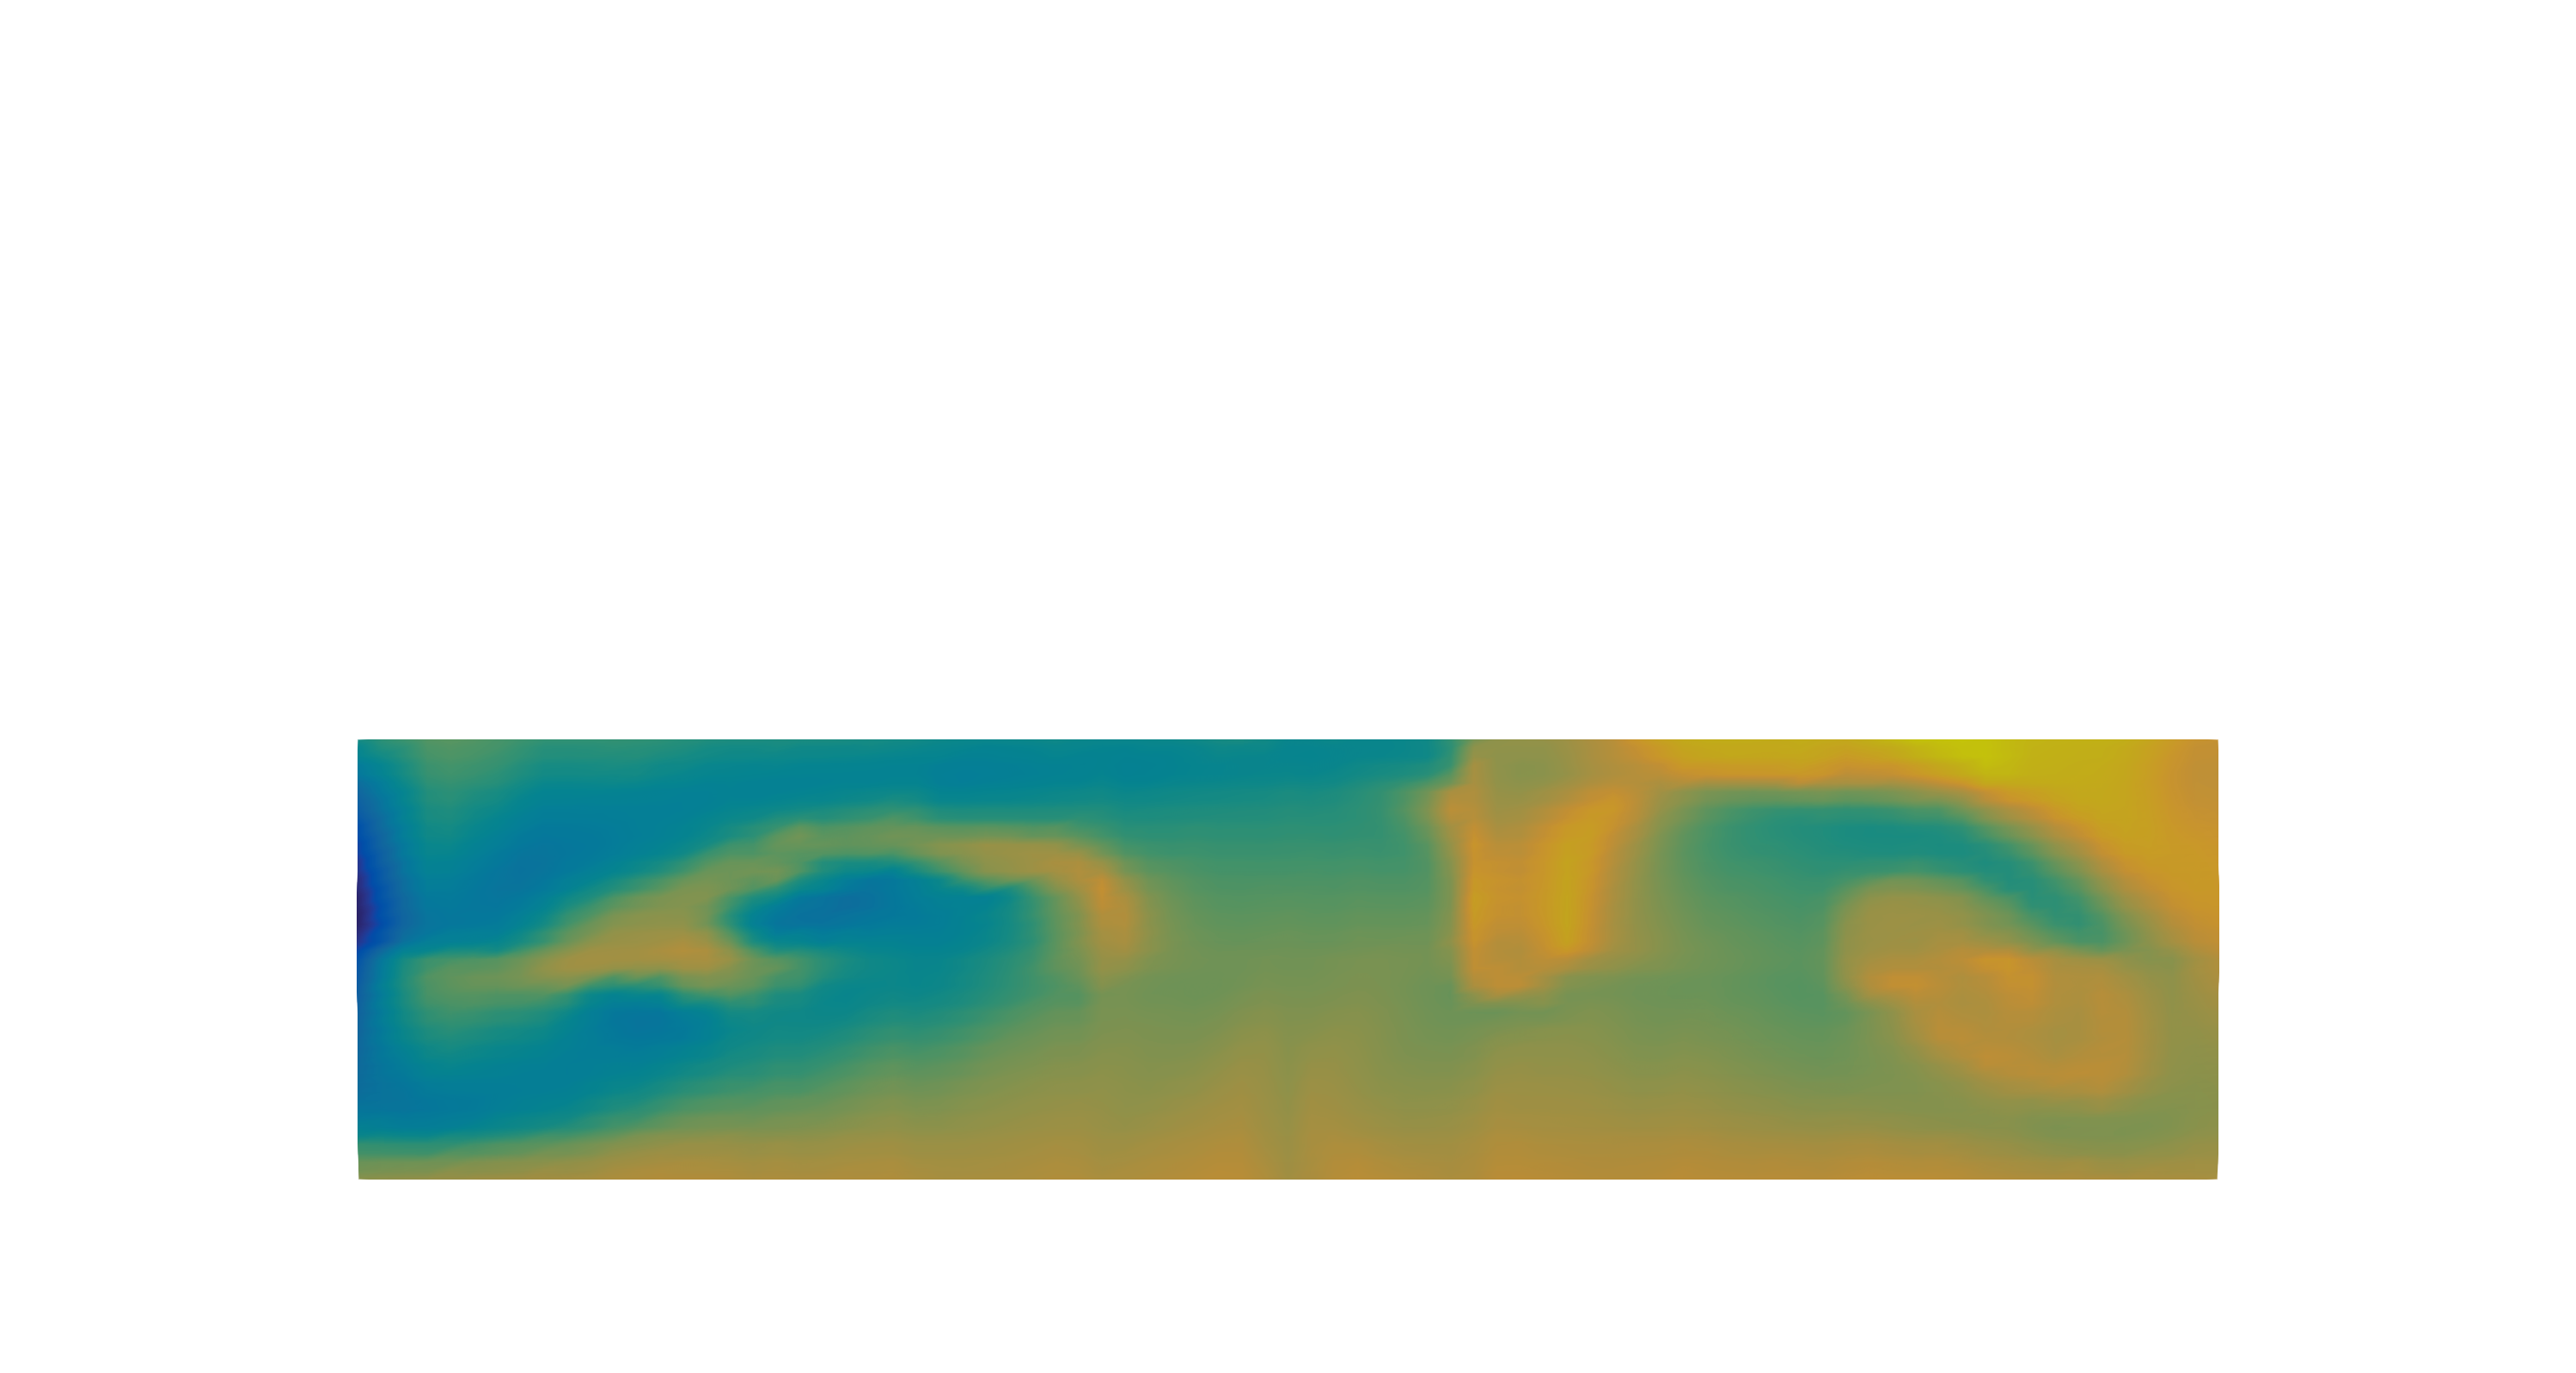
\includegraphics[width=\rasterimagewidth]{{../media/populations/application/print/alumina-influance-exp-2.55-3.08}.png}}};
        \end{axis}
      \end{tikzpicture}
    \caption{Champ de concentration $c$ dans l'ACD de la cuve AP32 à
      $t = $ \num{10000} \si{\second}. En haut, $T_\text{Crit} =
      T_\text{Liq}$. En bas, $T_\text{Crit} = T_\text{Liq} + 0.86$
      \si{\kelvin}.}
    \label{fig:dissolution-influence-exp-heaviside}
  \end{center}
\end{figure}


Dans la limite où $\tcrit - \tliq$ devient grand, on voit facilement
dans l'expression (\ref{eq:dissolution-rate}) que le taux de
dissolution des particules, et donc leur vitesse de dissolution,
devient nulle dans l'intervalle de température que le bain
électrolytique peut raisonnablement admettre. Par conséquent, si la
valeur de $\tcrit - \tliq$ est trop élevée, le temps dissolution des
particules peut devenir arbitrairement long, ce qui n'est pas réaliste
dans le cas d'une cuve d'électrolyse d'aluminium industrielle.

A l'inverse, en prenant la limite $\tcrit \to  \tliq$, le taux de
dissolution (\ref{eq:dissolution-rate}) s'écrit:
\begin{equation}\label{eq:dissolution-rate-zero-tcrit}
  \dissolutionrate(\concentration,\temperature) = \left\{
  \begin{array}{ll}
  K \displaystyle\frac{\csat - \concentration}{\csat}& \text{ si } \temperature
  \geq \tliq\text{ et } 0\leq \concentration \leq \csat,\\
  0 &  \text{ sinon.}
  \end{array}
  \right.
\end{equation}
En d'autres termes, la dissolution des particules est contrôlée
uniquement par la concentration locale $\concentration$ si
$\temperature \geq \tliq$, et les particules ne se dissolvent pas sinon.

Nous présentons maintenant la distribution de concentration d'alumine
dissoute dans le bain de la cuve AP32 dans l'état périodique résultant
de deux calculs. Comme précédemment, l'ensemble des paramètres du
modèle de transport et dissolution est reporté dans la table
\ref{tab:dissolution-physical-parameters}. Pour le premier calcul on
fixe $\tcrit = \tliq$, et le taux de dissolution est donné par
(\ref{eq:dissolution-rate-zero-tcrit}). Pour le deuxième calcul on
fixe $\tcrit = \tliq + 0.86$ \si{\kelvin}.

La figure \ref{fig:dissolution-influence-exp-heaviside} présente la
concentration d'alumine dans l'ACD de la cuve AP32 à $t = \num{10000}$
\si{\second}, lorsque l'état périodique est atteint. Le premier champ
de concentration correspond au cas où $\tcrit = \tliq$, tandis que le
deuxième champ de concentration correspond au cas où $\tcrit = \tliq +
0.86$ \si{\kelvin}. Même si l'on parvient à observer de petites
variations entre ces deux solutions, en particulier dans le coin aval
droite et autour du point d'injection \#4, ces deux champs de
concentration sont indistinguables l'un de l'autre.

Finalement, nous nous penchons sur l'effet de la chute
gravitationnelle des particules d'alumine sur le champ de
concentration d'alumine dissoute.

% Sensibilité par rapport a la vitesse de chute dans le bain
\paragraph{Effet de la vitesse de chute des particules sur leur
  dissolution}

Nous avons déterminé, dans la section \ref{sec:particle-fall}, la vitesse
de chute et la profondeur maximale atteinte dans le fluide des
particules soumisent à la gravité et à une force de traînée de
Stokes. Dans le cas le plus favorable, les particules de plus grande
taille peuvent chuter de plusieurs centimètres dans le bain
électrolytique avant de se dissoudre complètement.

Dans ce dernier paragraphe, nous proposons de comparer deux calculs
qui illustrent l'effet de la chute des particules dans le bain sur la
concentration d'alumine dissoute dans celui-ci.

Pour le premier calcul, qui joue le rôle de point de référence, les
paramètres sont reportés dans la table
\ref{tab:dissolution-physical-parameters} et nous annulons
l'accélération de la gravité $g = 0$, ce qui donne lieu à une vitesse
de chute strictement nulle, soit $w(r) = 0$ pour tout $r>0$. De plus,
l'injection des doses d'alumine a lieu dans le canal central comme
indiqué sur la figure \ref{fig:injections}, au niveau de l'ACD.

Pour le deuxième calcul la valeur de $g$ est restaurée, telle que
donnée dans la table \ref{tab:dissolution-physical-parameters} et la
vitesse de chute des particules est donnée par l'expression
\ref{eq:fall-velocity}. Cependant, les points d'injections sont
déplacés verticalement vers le haut du canal.

Nous avons montré dans la section \ref{sec:particle-fall} que les
profondeurs maximales atteintes par les particules lorsque la viscosité
du fluide est supérieure ou égale à \num{1e-2}
\si{\kilo\gram\per\meter\per\second} sont de l'ordre du
millimètre. Or, la taille verticale des mailles dans les canaux ne
permet pas de capturer des effets de cette amplitude. Pour cette
raison, nous choisissons pour le paramètre de viscosité
$\electrolyteviscosity$, qui intervient dans la définition
(\ref{eq:fall-velocity}), la viscosité laminaire du fluide, soit
$\electrolyteviscosity = $ \num{2e-3}
\si{\kilo\gram\per\meter\per\second}. Cette valeur de la viscosité
donne lieu à des profondeurs de chute maximale de particule dans le
bain de l'ordre de quelques centimètres.

La figure \ref{fig:sedimentation-comparaison} représente les champs de
concentration dans l'ACD de la cuve AP32 obtenus par ces deux calculs,
évalués à $t = \num{10000}$ \si{\second}, lorsque l'état périodique est
atteint.

\begin{figure}[!hp]
  \begin{center}
      \begin{tikzpicture}
        \begin{axis}[
            hide axis,
            %colorbar,
             scale only axis,
             height=0.41\rasterimagewidth,,
             width=\rasterimagewidth,
             %colorbar horizontal,
             point meta min=2.38,
             point meta max=4.21,
             colorbar style={
               title=Concentration [\%w],
               width=7.4cm,
               height=0.3cm,
               xtick={2.38, 3, 3.5, 4,4.21, 4.5, 5, 5.5, 6},
               at={(0.5\rasterimagewidth,0.4cm)},
               anchor=north
            }
          ]
          \addplot [] coordinates {(0,0)};
          \node (myfirstpic) at (0,0) {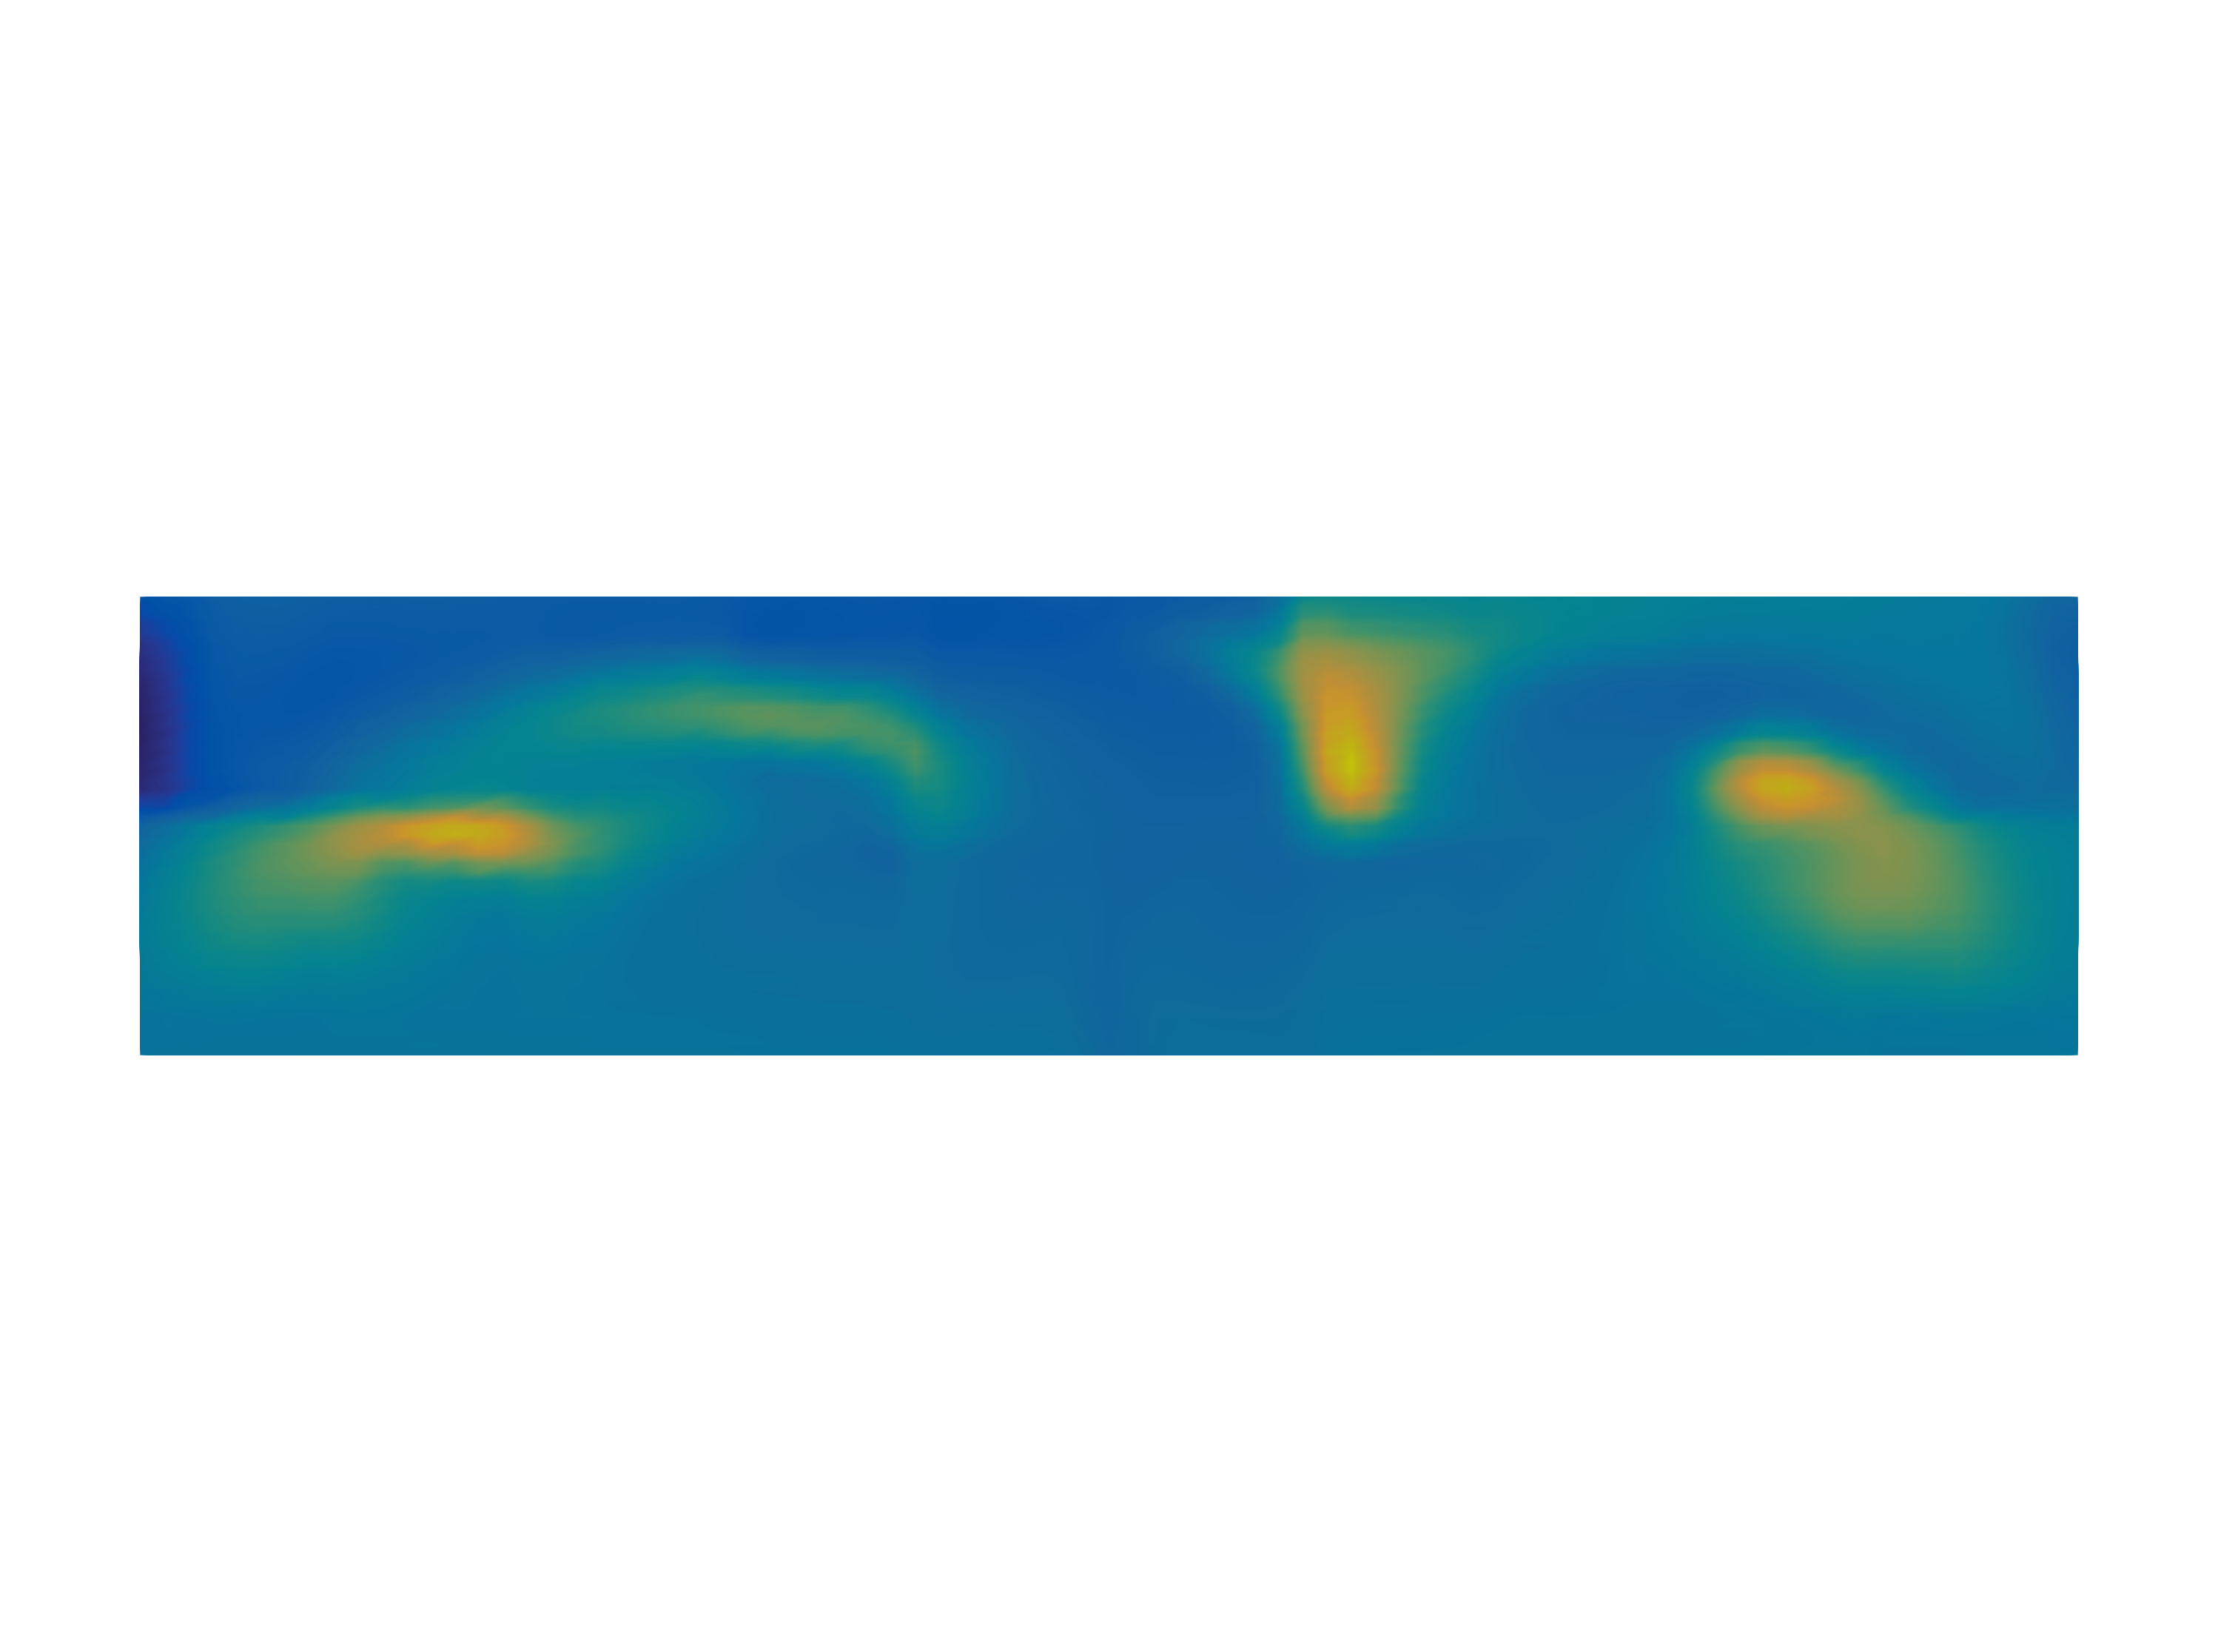
\includegraphics[width=\rasterimagewidth]{{../media/populations/application/print/alumina-control-2.38-4.21}.png}};
        \end{axis}
      \end{tikzpicture}
      \begin{tikzpicture}
        \begin{axis}[
            colorbar,
            hide axis,
            scale only axis,
            height=0.41\rasterimagewidth,
            width=\rasterimagewidth,
            colorbar horizontal,
            point meta min=2.38,
            point meta max=4.21,
            colorbar style={
              title=Concentration [\%w],
              width=7.4cm,
              height=0.3cm,
              xtick={2.38, 3, 3.5, 4,4.21, 4.5, 5, 5.5, 6},
              at={(0.5\rasterimagewidth,0.4cm)},
              anchor=north
            }
          ]
          \addplot [] coordinates {(0,0)};
          \node (myfirstpic) at (0,0) {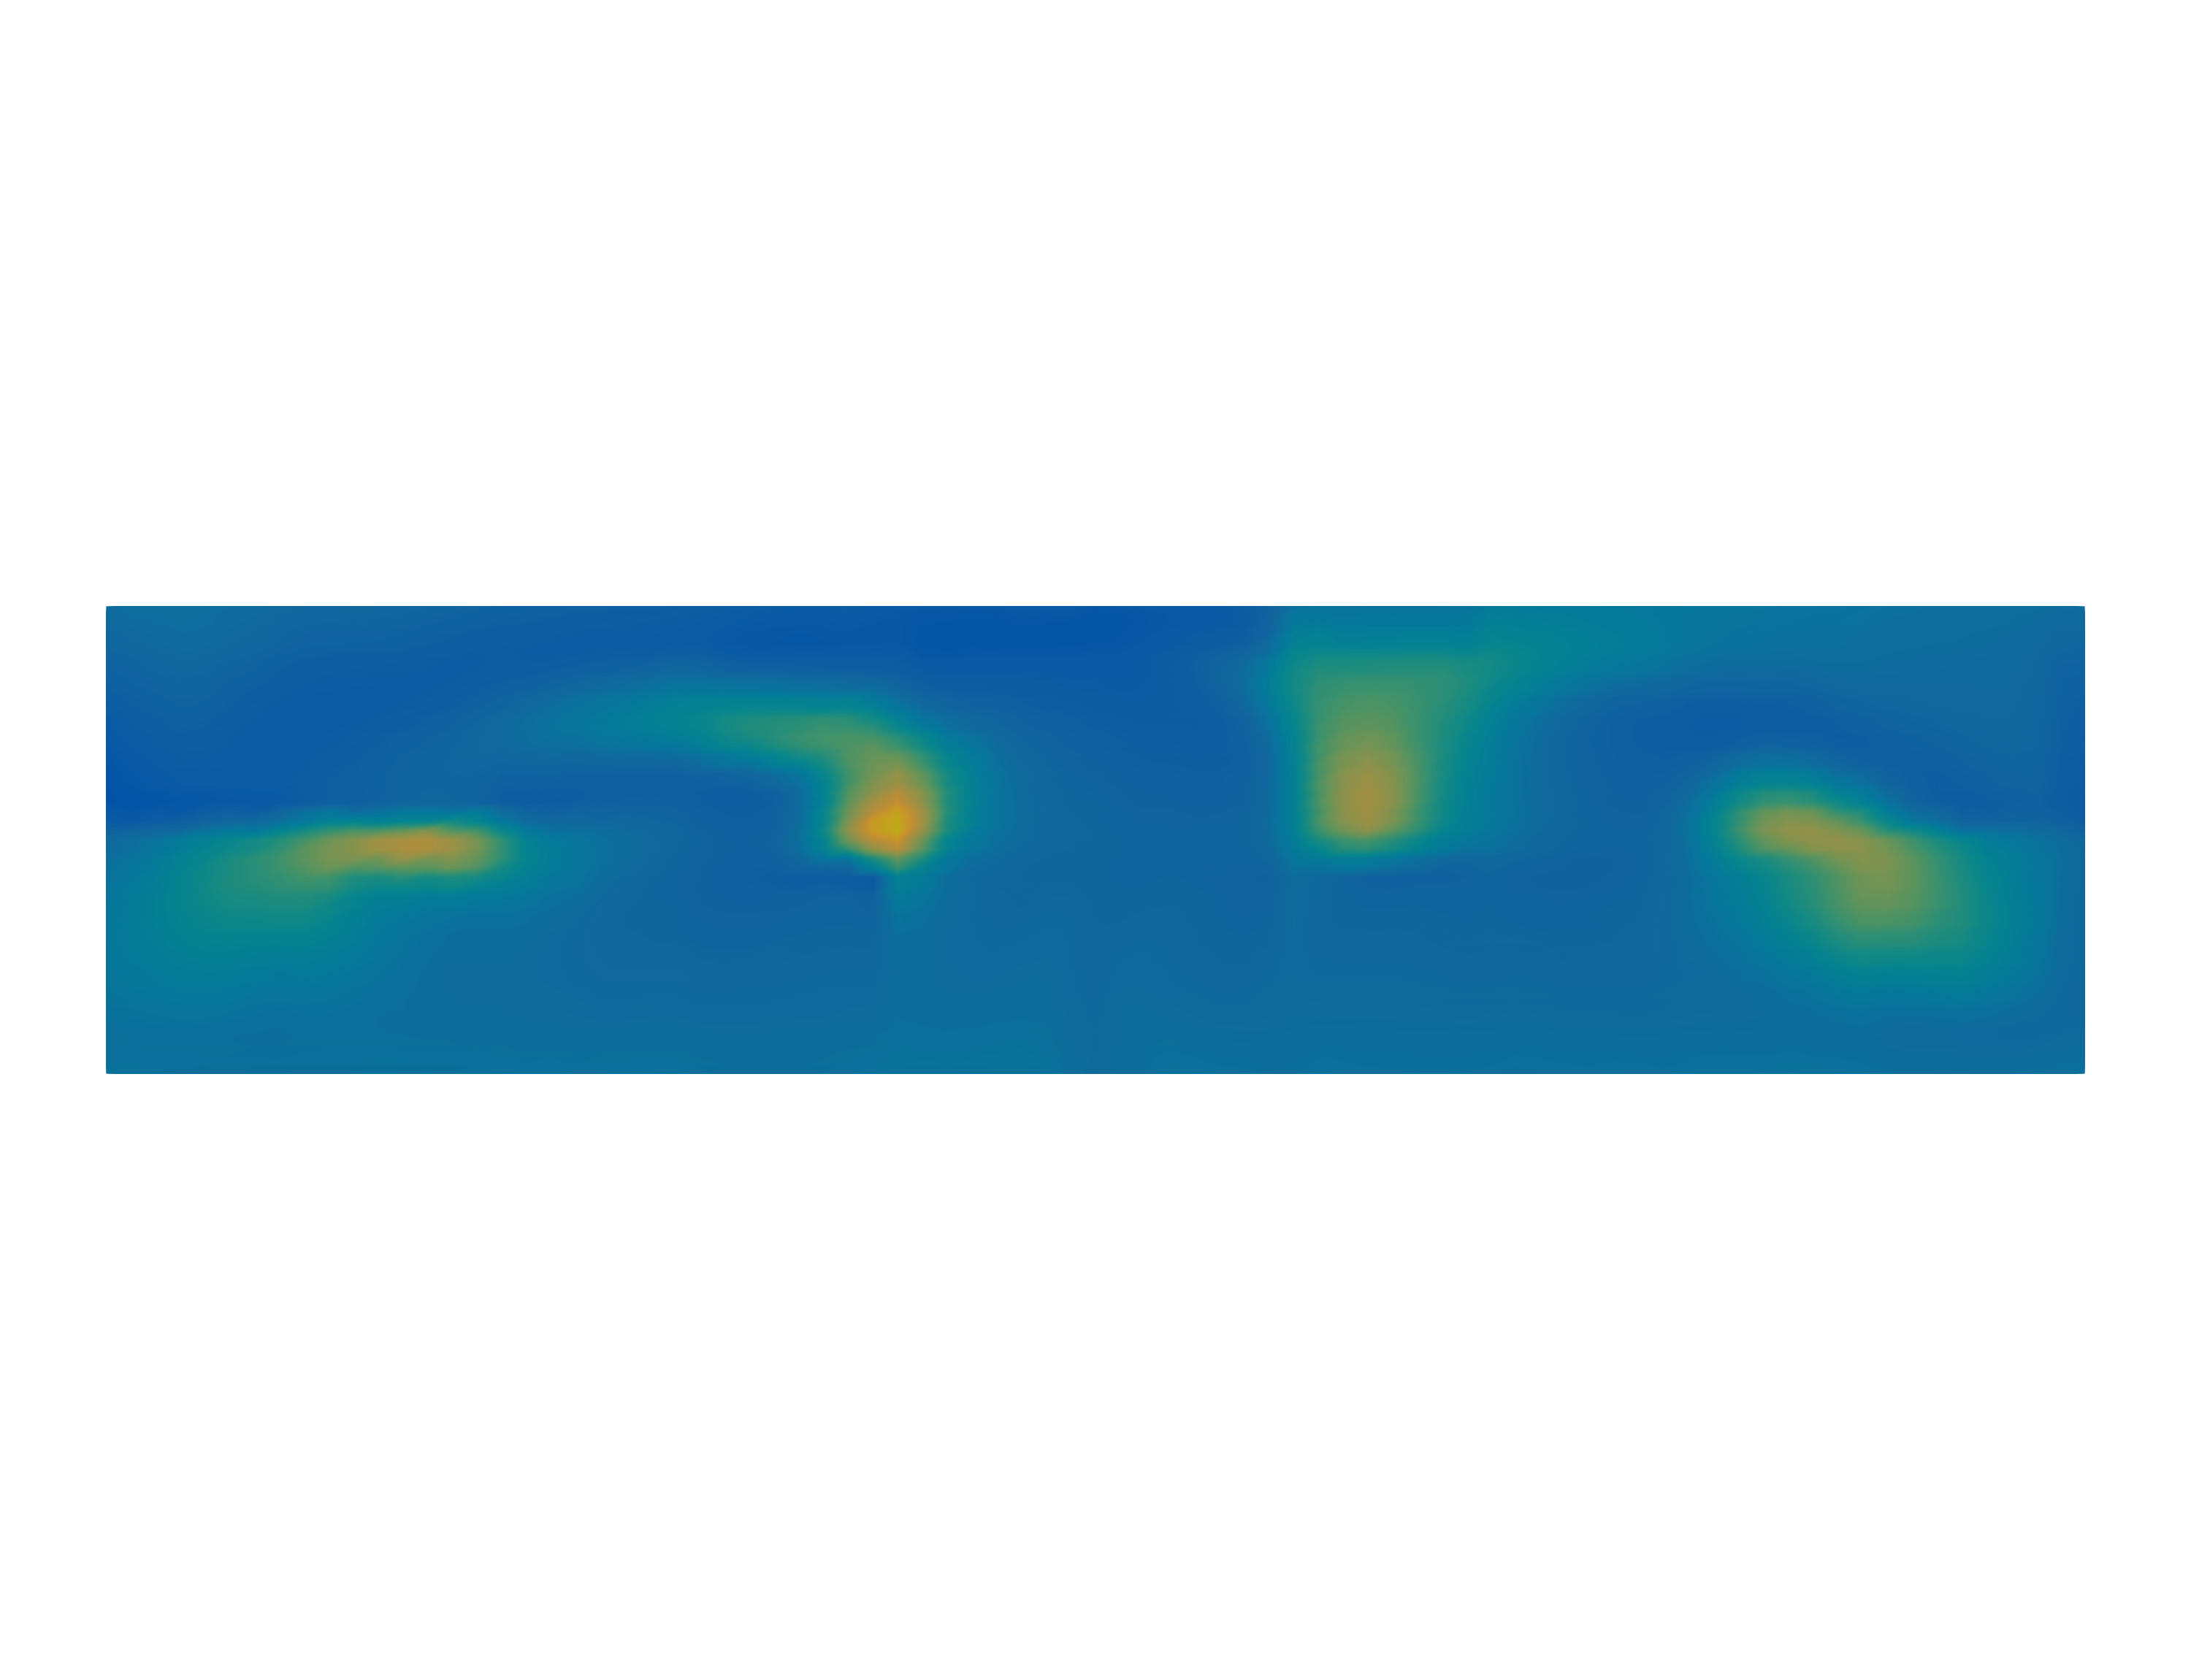
\includegraphics[width=\rasterimagewidth]{{../media/populations/application/print/dummy-tmp-result-c-2.38-4.21}.png}};
        \end{axis}
      \end{tikzpicture}
      \caption{Champ de concentration d'alumine dissoute dans l'ACD de
        la cuve AP32 à $t = \num{10000}\si\second$. En haut,
        dissolution des particules sans chute gravitationnelle dans le
        bain. En bas, dissolution des particules avec chute
        gravitationnelle dans le bain.}
      \label{fig:sedimentation-comparaison}
  \end{center}
\end{figure}


On remarque quelques différences entre les deux solutions,
essentiellement au niveau des points d'injection. Les valeur maximales
de la concentration d'alumine dissoute à proximité des points
d'injection \#1, \#3 et \#4 sont plus grandes lorsque lorsque la chute
des particules est négligée. On constate l'effet inverse pour
l'injecteur \#2: la concentration d'alumine dissoute sous cet
injecteur atteint un maximum local plus marqué lorsque la chute des
particules est pris en compte. Dans le reste du bain, la distribution
de concentration est similaire entre les deux calculs.

Nous concluons cette partie par une discussion de ces résultats.



\part{Approximation d'écoulement dans le bain électrolytique}
\label{part:fluid}

\chapter[Calcul de l'écoulement de Stokes]{Une méthode numérique pour le calcul de l'écoulement de Stokes}
\label{chap:fourier}
\section{Introduction}
\label{sec:fourier-introduction}
Comme annoncé dans le chapitre \ref{chap:introduction}, une cuve
d'électrolyse typique dans une halle de production n'est jamais dans
un état stationnaire \cite{Steiner2009}, \cite{Flotron2013}. La cause
majeure pour laquelle ces cuves se trouvent dans un état de
déséquilibre constant est due aux changements d'anodes en fin de vie,
qui interviennent toutes les 24 heures environ.

Cet état de déséquilibre entraîne d'importantes variation des
écoulements des fluides dans la cuve, et ces variations ont un impact
non négligeable sur la répartition de l'alumine dissoute dans le bain
électrolytique. Pour palier à ces variations de répartition d'alumine,
les opérateurs peuvent modifier les cadences d'injection de chaque
injecteur. Malheureusement, il ne disposent pour l'heure d'aucun outil
qui leur permette de déterminer comment adapter ces cadences en
fonction de l'état de la cuve.

Le modèle de dissolution et transport d'alumine proposé dans
\cite{Hofer2011} et dont nous avons étudié certaines extensions dans
la première partie de ce travail, offre un début de réponse: la
conductivité des différentes anodes dépend de leur âge, ce qui modifie
le champs de vitesse dans le bain électrolytique et dans l'aluminium
liquide, ainsi que la distribution d'alumine
dissoute. Malheureusement, ce calcul ne peut pas être fait en temps
réel, et donc la cadence des injecteurs qui optimise la répartition de
l'alumine dissoute dans le bain ne peut pas non plus être obtenu en
temps réel.

Dans ce chapitre nous proposons une méthode pour calculer le champ de
vitesse dans une cuve d'électrolyse bien plus rapidement qu'avec les
modèles de \cite{Steiner2009} et \cite{Hofer2011}, au prix de
certaines hypothèses supplémentaires que l'on discutera.

La géométrie d'une cuve d'aluminium est particulier: l'essentiel de
l'écoulement des fluides prend place dans un domaine
parallélépipédique qui présente une forte anisotropie. Les dimensions
horizontales ($\approx \num{14}\times\num{4}$ \si{\meter}) sont bien plus
grandes que la dimension verticales ($\approx \num{0.2}$ \si{\meter}). Par
conséquent, l'écoulement est essentiellement contraint dans le plan
horizontal, si l'on néglige ce qui se passe dans les canaux bien
entendu.

Le modèle de référence dans Alucell \cite{Steiner2009},
\cite{Flotron2013}, \cite{Hofer2011}, \cite{Rochat2016} calcule une
approximation des écoulements dans les fluides en utilisant une
méthode d'éléments finis Lagrange continu linéaire par morceau sur un
maillage en tétraèdre du domaine fluide.

Or, la géométrie anisotrope du domaine fluide d'une cuve d'électrolyse
pose de sérieuses difficultés au niveau numérique. En effet,
l'utilisation de mailles isotropes n'est pas possible puisque la
taille de maille dans la direction verticale est de l'ordre de
\num{0.01} \si{\meter}.

La seule alternative est de considérer des mailles anisotropes ed
l'ordre de \num{0.01} \si{\meter} dans la direction verticale et
\num{0.1} \si{\meter} dans les directions horizontales.

Cependant, l'utilisation de mailles anisotropes augmente le
conditionnement des matrices et donc le nombre d'itérations
nécessaires à la résolution du système linéaire et dégrade la
précision du calcul.

Le but de ce chapitre est de proposer une méthode pour calculer des
écoulements de Stokes ou de Navier-Stokes dans des domaines
parallélépipédiques présentant une forte anisotropie. Dans la section
\ref{sec:fourier-model} nous proposons une décomposition de Fourier de la
vitesse selon la direction verticale, puis nous proposerons dans la
section \ref{sec:fourier-discretisation} une méthode numérique de type éléments
finis pour approcher chaque harmonique de la décomposition de
Fourier. Dans la section \ref{sec:fourier-validation} nous validons
l'implémentation du schéma ainsi obtenu et étudions la convergence de
l'erreur par rapport à une solution non triviale. Finalement, dans la
section \ref{sec:fourier-application} nous appliquons cette méthode au
cas industriel d'une cuve d'électrolyse et évaluons les propriétés de
cette méthode.


\section{Formulation du modèle de Stokes Fourier}
\label{sec:fourier-model}
Soit $\Lambda$ un ouvert borné de $\mathbb R^2$ de bord Lipschitzien
$\partial\Lambda$. Soit $\thickness > 0$ un nombre réel donné
correspondant à la dimension verticale d'une cuve. On définit le
domaine de $\mathbb R^3$ correspondant à une simplification
géométrique de la cuve d'électrolyse
\begin{equation}\label{eq:domain}
  \Omega = \Lambda \times (0,\thickness).
\end{equation}
On suppose que le domaine $\Omega$ est occupé par l'électrolyte, un
fluide newtonien incompressible de viscosité tensorielle $\mu$. On suppose de plus
que le tenseur de viscosité est tel que:
\begin{itemize}
  \item $\mu$ est symétrique, \ie, $\mu_{ij} = \mu_{ji}$, $1\leq
    i,j\leq 3$,
  \item $\exists \chi_0 > 0$ tel que $\mu_{ij} > \chi_0$, $1\leq
    i,j\leq 3$,
    \item $\mu$ est indépendent de $x_3$.
\end{itemize}
Si $u$ est la
vitesse de l'écoulement, le tenseur des contraintes visqueuses dans le
fluide \cite{Landau1987} est donné par
\begin{equation}
  \stresstensor_{i,j}(u) = 2\electrolyteviscosity_{i,j}
  \straintensor_{i,j}(u),\quad i,j = 1,2,3.
\end{equation}
Ici on a noté $\straintensor$ le tenseur du taux de déformation du
fluide qui s'écrit en fonction de la vitesse d'écoulement $u$:
\begin{equation}
  \straintensor_{i,j}(u) = \frac{1}{2}\parent{\frac{\partial u_i}{\partial x_j} + \frac{\partial u_j}{\partial x_i}},\quad i,j = 1,2,3.
\end{equation}
Étant donné un champ de forces $f:\Omega\to \mathbb R^3$, on suppose
que la vitesse d'écoulement $u:\Omega \to \mathbb R^3$ et la pression
$p:\Omega \to \mathbb R$ du fluide satisfont le système de Stokes stationnaire
\begin{align}
  &- \div(\stresstensor(u)) + \nabla p = f,\label{eq:stokes-u}\\
  &\div \parent{u} = 0\label{eq:stokes-p}
\end{align}
dans $\Omega$. Dans la suite nous noterons $u = (u_1, u_2, u_3)$ et $f =
(f_1, f_2, f_3)$. De plus, on demande à ce que l'écoulement $u$ satisfasse
les conditions aux limites suivantes. Sur les faces latérales, la
vitesse satisfait la condition d'adhérence
\begin{equation}
  u = 0\quad \text{ sur } \quad\partial \Lambda\times(0,\thickness).\label{eq:stokes-bc-1}
\end{equation}
Sur les faces horizontales supérieures et inférieures, la vitesse
d'écoulement satisfait une condition de glissement total. On a
\begin{align}
  &u_3(x_1, x_2, x_3) = 0,\label{eq:stokes-bc-2}\\
  &\parent{\stresstensor(u)\cdot \nu}\cdot t_i = 0,\quad i = 1,2\label{eq:stokes-bc-3}
\end{align}
sur $\Lambda \times\cparent{0,\thickness}$, avec $t_1$, $t_2$ les deux
vecteurs tangents unités.
Les conditions (\ref{eq:stokes-bc-2}), (\ref{eq:stokes-bc-3})
correspondent à demander à ce que le fluide ne pénètre pas les faces
horizontales de $\partial\Omega$ et à ce que les contraintes
tangentielles sur ces faces soient nulles. En utilisant
(\ref{eq:stokes-bc-2}), la condition (\ref{eq:stokes-bc-3}) se réécrit
\begin{equation}
\frac{\partial u_1}{\partial x_3} + \frac{\partial u_3}{\partial x_1}
  = 0 \quad \text{et} \quad \frac{\partial u_2}{\partial x_3} + \frac{\partial u_3}{\partial x_2}
  = 0\quad \text{ sur }\quad\partial \Lambda \times\cparent{0,\thickness}.
\end{equation}

\paragraph{Décomposition en séries de Fourier}
Pour résoudre le système d'équations (\ref{eq:stokes-u}),
(\ref{eq:stokes-p}) avec les conditions aux limites (\ref{eq:stokes-bc-1}) à
(\ref{eq:stokes-bc-3}), on exprime les inconnues sous forme de séries
de Fourier dans la direction $x_3$. Soit le domaine $\Omega^+ = \Lambda
\times (-\thickness, \thickness)$, on définit les fonctions suivantes
$\forall (x_1, x_2, x_3)\in \Omega^+$:
\begin{align}
  & U_i(x_1, x_2, x_3) = \left\{
    \begin{array}{lll}
      u_i(x_1, x_2, x_3) &\text{ si } x_3 \geq 0,\\
      u_i(x_1, x_2, -x_3) &\text{ si } x_3 < 0,     & \quad i = 1,2,
    \end{array}
  \right.\label{eq:decomp-1}\\
  %
  & U_3(x_1, x_2, x_3) = \left\{
    \begin{array}{ll}
       u_3(x_1, x_2, x_3) &\text{ si } x_3 \geq 0,\\
      -u_3(x_1, x_2, -x_3) &\text{ si } x_3 < 0,
    \end{array}
  \right.\label{eq:decomp-2}\\
  %
  & P(x_1, x_2, x_3) = \left\{
    \begin{array}{ll}
      p(x_1, x_2, x_3) &\text{ si } x_3 \geq 0,\\
      p(x_1, x_2, -x_3) &\text{ si } x_3 < 0,
    \end{array}
  \right.\label{eq:decomp-3}\\
  %
  & F_i(x_1, x_2, x_3) = \left\{
    \begin{array}{lll}
      f_i(x_1, x_2, x_3) &\text{ si } x_3 \geq 0,\\
      f_i(x_1, x_2, -x_3) &\text{ si } x_3 < 0,     & \quad i = 1,2,
    \end{array}
  \right.\label{eq:decomp-4}\\
  %
  & F_3(x_1, x_2, x_3) = \left\{
    \begin{array}{ll}
      f_3(x_1, x_2, x_3) &\text{ si } x_3 \geq 0\\
     -f_3(x_1, x_2, -x_3) &\text{ si } x_3 < 0.
    \end{array}
  \right.\label{eq:decomp-5}
\end{align}
En vertu de (\ref{eq:stokes-bc-2}) et (\ref{eq:stokes-bc-3}), les
dérivées selon $x_3$ des fonctions $U_1$, $U_2$ et $U_3$ ainsi
définies ne présentent pas de masse de Dirac en $x_3 = 0$. La figure
\ref{fig:solution-periodique} représente schématiquement le
comportement et la régularité de ces fonctions de part et d'autre de
l'origine de l'axe $x_3$.

\begin{figure}
  \begin{center}
    \input{../media/fourier/solution-periodique/solution-periodique.pdf_tex}
    \caption{Représentation schématique de la réplication des fonction
    $u_i$, $i = 1,2,3$, $p$, et $f_i$, $i = 1,2,3$ sur l'intervalle
      $(0, -\thickness)$. En $x_3 = 0$, les fonctions $U_i$,
      $i=1,2,3$ sont $\mathcal C^1$, $P$, $F_1$, $F_2$ sont $\mathcal
      C^0$, et $F_3$ est discontinue.}
    \label{fig:solution-periodique}
  \end{center}
\end{figure}


Avec les définitions ci-dessus on vérifie que $U = (U_1, U_2, U_3)$ et
$P$ satisfont les équations
\begin{align}
  &-\div\parent{\mathcal T(U)} + \nabla P = F,\label{eq:stokes-periodic-1}\\
  &\div\parent{U} = 0\label{eq:stokes-periodic-2}
\end{align}
dans $\Omega^+$. De plus on a
\begin{equation}
U_3 = 0 \quad\text{ sur } \Lambda\times \cparent{-\thickness} \text{ et } \Lambda\times \cparent{\thickness}
\end{equation}
et
\begin{equation}
  \frac{\partial U_i}{\partial x_3} = 0\quad \text{ sur } \Lambda\times
  \cparent{-\thickness} \text{ et } \Lambda\times \cparent{\thickness}
\end{equation}
pour $i = 1,2$, c'est-à-dire que
\begin{equation}
\parent{\stresstensor(U)\cdot \nu}\cdot t_i = 0\quad i = 1,2, \text{ sur } \Lambda\times
\cparent{-\thickness, \thickness}.
\end{equation}

On prolonge toutes les fonctions dans la variable $x_3$ sur tout
$\mathbb R$ en des fonctions périodiques de période $2\thickness$ en
$x_3$. On note encore par $U_1$, $U_2$, $U_3$, $P$, $F_1$, $F_2$,
$F_3$ ces prolongements, c'est-à-dire que ces fonctions sont
considérées comme fonctions de $(x_1, x_2, x_3)\in \Lambda\times
\mathbb R$ et $2\thickness$-périodiques selon $x_3$. Les fonctions
$U_1$, $U_2$, $U_3$ sont $\mathcal C^2$ par morceaux, $P$ est
$\mathcal C^1$ par morceaux et $F_1$, $F_2$, $F_3$ sont $C^0$ par
morceaux.

On pose pour alléger l'écriture $\beta^k = \frac{\pi
k}{\thickness}$. Les décompositions en séries de Fourier selon la
variable $x_3$ des fonctions $U_i$, $F_i$, $i = 1,2,3$ et $P$ s'écrivent
\begin{align}
  &U_i(x_1, x_2, x_3) = u_i^0(x_1, x_2) %
                       + \sum_{k > 0} u_i^k(x_1, x_2)%
                       \cos\parent{\beta^kx_3}, &\quad i = 1, 2,\label{eq:fourier-coeff-def-1}\\
  &U_3(x_1, x_2, x_3) = \sum_{k > 0} u_3^k(x_1, x_2)%
                        \sin\parent{\beta^kx_3},\label{eq:fourier-coeff-def-2}\\
  &P(x_1, x_2, x_3) = p^0(x_1, x_2) %
                      + \sum_{k>0}p^k(x_1, x_2)%
                      \cos\parent{\beta^kx_3},\label{eq:fourier-coeff-def-3}\\
  &F_i(x_1, x_2, x_3) = f_i^0(x_1, x_2) %
                        + \sum_{k > 0}f_i^k(x_1, x_2)%
                        \cos\parent{\beta^kx_3}, &\quad i = 1,2,\label{eq:fourier-coeff-def-4}\\
  &F_3(x_1, x_2, x_3) = \sum_{k > 0}f_3^k(x_1,x_2)%
                        \sin\parent{\beta^kx_3}.\label{eq:fourier-coeff-def-5}
\end{align}
On note $u^0 = (u^0_1, u^0_2)$, $f^0 = (f^0_1, f^0_2)$, $u^k =
(u^k_1,u^k_2,u^k_3)$ et $f^k = (f^k_1, f^k_2, f^k_3)$, $k \geq 1$. On
obtient les équations que les coefficients de Fourier $u^k$, $p^k$,
$k>0$ doivent satisfaire en substituant les définitions
(\ref{eq:fourier-coeff-def-1}) à (\ref{eq:fourier-coeff-def-5}) dans
le système d'équation de Stokes
(\ref{eq:stokes-periodic-1}),(\ref{eq:stokes-periodic-2}). Les bases
de Fourier $\cparent{\cos(\beta^k x_3)}_{k > 0}$ et
$\cparent{\sin(\beta^kx_3)}_{k>0}$ sur $\mathbb R$ étant
respectivement orthogonales, on peut identifier les équations pour
chaque mode indépendamment des autres. On obtient pour $k = 0$:
\begin{align}
  &-\sum_{j = 1}^2\frac{\partial}{\partial
    x_j}\parent{\mu_{ji}\parent{\frac{\partial u_i^0}{\partial x_j} +
      \frac{\partial u_j^0}{\partial x_i}}} + \frac{\partial
    p^0}{\partial x_i} = f_i^0, \quad i = 1,2,\label{eq:fourier-fund-1}\\
  &\sum_{j = 1}^2 \frac{\partial u_j^0}{\partial x_j} = 0\label{eq:fourier-fund-2}
\end{align}
sur $\Lambda$ et $u^0 = 0$ sur $\partial \Lambda$.

On obtient pour $k
\geq 1$:
\begin{align}
  &-\sum_{j = 1}^2\frac{\partial}{\partial
    x_j}\parent{\mu_{ji}\parent{\frac{\partial u_i^k}{\partial x_j} +
      \frac{\partial u_j^k}{\partial x_i}}} -
  \mu_{3i}\parent{\beta^k\frac{\partial u_3^k}{\partial x_i} -
    \parent{\beta^k}^2 u_i^k} + \frac{\partial p^k}{\partial x_i} = f_i^k,\quad
  i = 1,2,\label{eq:fourier-harm-1}\\
  &-\sum_{j = 1}^2\frac{\partial}{\partial
    x_j}\parent{\mu_{j3}\parent{\frac{\partial u_3^k}{\partial x_j} -
      \beta^k u_j^k}} + 2\mu_{33}\parent{\beta^k}^2 u_3^k - \beta^k p^k =
  f_3^k,\label{eq:fourier-harm-2}\\
  &\sum_{j = 1}^2\frac{\partial u_j^k}{\partial x_j} + \beta^k u_3^k = 0\label{eq:fourier-harm-3}
\end{align}
sur $\Lambda$ et $u^k = 0$ sur $\partial \Lambda$.

Étant données les forces $F_i$, $i = 1,2,3$, les coefficients $f^k$,
$k \geq 0$ qui apparaissent dans les membres de droite des équations
(\ref{eq:fourier-fund-1}), (\ref{eq:fourier-harm-1}) et
(\ref{eq:fourier-harm-2}) s'obtiennent par une projection $\mathrm
L^2$ sur la base de Fourier correspondante. Pour $k = 0$ on a
\begin{align}
  f_i^0(x_1, x_2) &=
  \frac{1}{2\thickness}\int_{-\thickness}^{\thickness}F_i(x_1, x_2, x_3)\,\mathrm
  dx_3, \quad i = 1,2,\nonumber\\
  &= \frac{1}{\thickness}\int_{0}^{\thickness}f_i(x_1, x_2, x_3)\,\mathrm
  dx_3, \quad i = 1,2,\label{eq:f-1}
\end{align}
et pour $k > 0$ on a
\begin{align}
f_i^k(x_1, x_2) &=
\frac{1}{\thickness}\int_{-\thickness}^{\thickness}F_i(x_1, x_2,
x_3)\cos\parent{\beta^k x_3}\,\mathrm dx_3,\quad i =
1,2,\\
&=
\frac{2}{\thickness}\int_{0}^{\thickness}f_i(x_1, x_2,
x_3)\cos\parent{\beta^k x_3}\,\mathrm dx_3,\quad i =
1,2,\label{eq:f-2}\\
f_3^k(x_1, x_2) &= \frac{1}{\thickness}\int_{-\thickness}^{\thickness}
F_3(x_1, x_2,x_3) \sin\parent{\beta^k x_3}\,\mathrm
dx_3,\\
&= \frac{2}{\thickness}\int_{0}^{\thickness}
f_3(x_1, x_2,x_3) \sin\parent{\beta^k x_3}\,\mathrm
dx_3.\label{eq:f-3}
\end{align}


\paragraph{Formulation faible}\label{sec:stokes-fourier-weak}
Nous énonçons maintenant les formulations variationnelles du problème
formé par les équations (\ref{eq:fourier-fund-1}) et
(\ref{eq:fourier-fund-2}) qui correspondent au mode fondamental de
l'écoulement $u$, et des problèmes formés par les équations
(\ref{eq:fourier-harm-1}) à (\ref{eq:fourier-harm-3}) qui
correspondent à chacune des harmoniques de l'écoulement $u$. Pour ce
faire, nous aurons besoin des espaces fonctionnels suivants. L'espace
$L^2(\Lambda)$ est l'ensemble
\begin{align}
  L^2(\Lambda) = \cparent{f:\Lambda\to\mathbb R \mathrel{\Big|} \int_\Lambda
    \abs{f}^2\mathrm dx < \infty}.
\end{align}
Il est muni du produit scalaire
\begin{align}
  (f, g)_{L^2(\Lambda)} = \int_\Lambda f(x)g(x)\mathrm dx
\end{align}
pour tout $f, g\in L^2(\Lambda)$, et de la norme
\begin{align}
  \norm{f}_{L^2(\Lambda)} = \sqrt{(f, f)_{L^2(\Lambda)}}\quad\forall f\in L^2(\Lambda).
\end{align}
On notera encore $H^1(\Lambda)$ l'espace de Sobolev
$W^{1,2}(\Lambda)$, c'est-à-dire que
\begin{align}
  H^1(\Lambda) = \cparent{f\in L^2(\Lambda)\mathrel{\bigg|} \int_\Lambda
    \abs{\nabla f}^2 \mathrm dx < \infty}
\end{align}
et
\begin{align}
  H^1_0(\Lambda) = \cparent{f \in H^1(\Lambda) \mathrel{\bigg|}
    f|_{\partial \Lambda} = 0}.
\end{align}
Nous aurons finalement besoin des espaces de fonctions à moyenne nulle
\begin{align}
  &L^2_0(\Lambda) = \cparent{f\in L^2(\Lambda)\mathrel{\bigg|}
    \int_\Lambda f \,\mathrm dx = 0},\\
  \text{et }\quad &H^1_{0,0}(\Lambda) = \cparent{f\in H^1_0(\Lambda)\mathrel{\bigg|}
    \int_\Lambda f \,\mathrm dx = 0}.
\end{align}
Remarquons que $L^2_0(\Lambda)$ est un sous-espace fermé de
$L^2(\Lambda)$ et $H^1_{0,0}(\Lambda)$ est un sous-espace fermé de
$H^1_0(\Lambda)$ ce qui sera important pour répondre aux questions
d'existence et d'unicité par la suite.

Commençons tout d'abord par traiter le mode fondamental. Pour
simplifier l'écriture, on note $\overline{\mu}$ et
$\reducedstraintensor$ la viscosité et le tenseur du taux de
déformation réduits aux composantes 1 et 2:
\begin{equation}
 \overline{\mu} = \begin{bmatrix}
  \mu_{1,1} & \mu_{1,2} \\
  \mu_{2,1} & \mu_{2,2}
 \end{bmatrix},\quad \text{et} \quad \reducedstraintensor_{ij}(u) =
 \straintensor_{ij}(u),\ i,j = 1,2.
\end{equation}
Le problème faible correspondant aux équations
(\ref{eq:fourier-fund-1}) et (\ref{eq:fourier-fund-2}) consiste à
chercher les fonctions $u_1^0,u_2^0 \in H^1_0(\Lambda)$, $p^0 \in
L^2_0(\Lambda)$, telles que
\begin{align}
  &\int_\Lambda \electrolyteviscosity\otimes \reducedstraintensor(u^0) : \reducedstraintensor(v) \intd{x_1}\intd{x_2} -
  \int_\Lambda p^0\div v \intd{x_1}\intd{x_2} = \int_\Lambda f^0\cdot v
  \intd{x_1}\intd{x_2},\label{eq:fourier-weak-fund-1}\\
  &\int_\Lambda q\div u^0 \intd{x_1}\intd{x_2} = 0,\label{eq:fourier-weak-fund-2}
\end{align}
pour toutes fonctions $v \in \parent{H^1_0(\Lambda)}^2$, $q \in
L_0^2(\Lambda)$. Ici $\otimes$ est le produit tensoriel, \ie,
$\parent{\mu\otimes\reducedstraintensor}_{i,j} =
\mu_{ij}\reducedstraintensor_{ij}$ et $\mu\otimes\reducedstraintensor(u):\reducedstraintensor(v) =
\sum_{i,j = 1}^2\mu_{ij}\reducedstraintensor_{ij}(u)\reducedstraintensor_{ij}(v)$.
En admettant que $\partial \Lambda$ est Lipschitzien et en supposant
que $f^0\in \mathrm L^2(\Lambda)$, il est connu que la formulation
faible (\ref{eq:fourier-weak-fund-1}),(\ref{eq:fourier-weak-fund-2})
admet une unique solution \cite{Temam1977}.

Traitons à présent les problèmes pour les coefficients $u^k$ et
$p^k$. Soit $k > 0$ et soit $\tilde \straintensor^k$ le tenseur $3\times
3$ défini par
\begin{equation}
  \tilde\straintensor^k(u) = \begin{bmatrix}
     2\frac{\partial u_1}{\partial x_1}
    & \frac{\partial u_1}{\partial x_2} + \frac{\partial u_2}{\partial x_1}
    & \frac{\partial u_3}{\partial x_1} - \beta_k u_1 \\
    %
       \frac{\partial u_2}{\partial x_1} + \frac{\partial u_1}{\partial x_2}
    & 2\frac{\partial u_2}{\partial x_2}
    &  \frac{\partial u_3}{\partial x_2} - \beta_k u_2 \\
    %
       \frac{\partial u_3}{\partial x_1} - \beta_k u_1
    &  \frac{\partial u_3}{\partial x_2} - \beta_k u_2
    & 2\beta_k u_3
  \end{bmatrix}
\end{equation}
On obtient la formulation faible pour chaque harmonique en multipliant
les équations (\ref{eq:fourier-harm-1}) à (\ref{eq:fourier-harm-3})
par des fonctions test $v_1$, $v_2$, $v_3$ et $q$ et en intégrant par
parties les termes qui comportent des dérivées secondes. Le problème
faible pour chaque harmonique $k$ consiste à chercher les fonctions
$u^k = (u_1^k,u_2^k,u_3^k)\in \parent{H^1_0(\Lambda)}^3$ et $p^k\in
L^2(\Lambda)$ telles que
\begin{align}
  &\int_\Lambda 2\mu\otimes\tilde\straintensor^k(u^k):\tilde\straintensor^k(v)
  - \int_\Lambda p^k\parent{\frac{\partial v_1}{\partial x_1} +
    \frac{\partial v_2}{\partial x_2} + \beta^k v_3}
  = \int_\Lambda f^k\cdot v,\label{eq:fourier-weak-harm-1}\\
  &\int_\Lambda \parent{\frac{\partial u_1^k}{\partial x_1} + \frac{\partial u_2^k}{\partial x_2} + \beta^k u_3^k}q = 0\label{eq:fourier-weak-harm-2}
\end{align}
pour toutes fonctions $v = (v_1,v_2,v_3)\in \parent{H^1_0(\Lambda)}^3$
et $q\in L^2(\Lambda)$. Ici on adopte les mêmes notations que
précédemment pour le produit tensorielle avec $i,j =
1,2,3$. Remarquons que l'on omet $\intd{x_1}\intd{x_2}$ dans les
intégrales pour simplifier l'écriture. Nous reformulons maintenant ce
problème sous une forme plus adéquate pour l'analyse qui suit.  On
montre en utilisant le théorème de la divergence et en posant $\tilde
p^k = p^k - C^k$ avec $C^k = \abs{\Lambda}^{-1} \int_\Lambda
p^k\intd{x_1}\intd{x_2}$ que le problème
(\ref{eq:fourier-weak-harm-1}),(\ref{eq:fourier-weak-harm-2}) est
équivalent au problème suivant: trouver $u^k\in H^1_0(\Lambda)^3$,
$\tilde p^k \in L^2_0(\Lambda)$ et $C^k\in\mathbb R$ tels que pour
tout $v\in H^1_0(\Lambda)^3$ et $q \in L^2_0(\Lambda)$:
\begin{align}
  &\int_\Lambda 2\mu\otimes\tilde\straintensor^k(u^k):\tilde\straintensor^k(v)
  - \int_\Lambda \tilde p^k\parent{\frac{\partial v_1}{\partial x_1} +
    \frac{\partial v_2}{\partial x_2}} - \int_\Lambda(\tilde p^k +
  C^k)\beta^k v_3
  = \int_\Lambda f^k\cdot v,\label{eq:fourier-weak-harm-v2-1}\\
  &\int_\Lambda \parent{\frac{\partial u_1^k}{\partial x_1} +
    \frac{\partial u_2^k}{\partial x_2} + \beta^k u_3^k}q =
  0,\label{eq:fourier-weak-harm-v2-2}\\
  &\int_\Lambda u_3^k = 0.\label{eq:fourier-weak-harm-v2-3}
\end{align}
Soit maintenant $\psi \in H^1_0(\Lambda)$ tel que $\int_\Lambda
\psi\,\mathrm dx \neq 0$. Alors on peut écrire $H^1_0(\Lambda) =
H^1_{0,0}(\Lambda) \oplus W$, où $W =\mathrm{span}(\psi)$. En
cherchant $u_3^k \in H^1_{0,0}(\Lambda)$ (voir éq. (\ref{eq:fourier-weak-harm-v2-3})), on obtient
le problème que l'on montrera bien posé suivant: trouver $u^k \in
H_0^1(\Lambda)^2 \times H_{0,0}^1(\Lambda)$, $\tilde p^k \in
L^2_0(\Lambda)$ tels que pour tout $v \in H_0^1(\Lambda)^2 \times
H_{0,0}^1(\Lambda)$, $q \in L^2_0(\Lambda)$ on ait
\begin{align}
  &\int_\Lambda 2\mu\otimes\tilde\straintensor^k(u^k):\tilde\straintensor^k(v)
  - \int_\Lambda \tilde p^k\parent{\frac{\partial v_1}{\partial x_1} +
    \frac{\partial v_2}{\partial x_2} + \beta^k v_3}
  = \int_\Lambda f^k\cdot v,\label{eq:fourier-weak-harm-v3-1}\\
  &\int_\Lambda \parent{\frac{\partial u_1^k}{\partial x_1} + \frac{\partial u_2^k}{\partial x_2} + \beta^k u_3^k}q = 0\label{eq:fourier-weak-harm-v3-2}
\end{align}
La constante $C^k$ est unique et peut être calculée a posteriori en
connaissant les fonctions $u^k$ et $\tilde p^k$. Nous reportons la
discussion de ce point à la fin de cette section.

Afin de rendre plus explicite la structure sous-jacente de cette
formulation, on peut l'exprimer en des termes plus abstraits. Notons
$V = H^1_0(\Lambda)^2\times H^1_{0,0}(\Lambda)$. Soit $a^k:V\times V
\to \mathbb R$ les formes bilinéaires continues définies pour tout $k
> 0$ par
\begin{equation}
  a^k(u,v) = \int_\Lambda
  2\mu\otimes\tilde\straintensor^k(u):\tilde\straintensor^k(v)
\end{equation}
et les formes bilinéaires continues $b^k:V\times L^2_0(\Lambda)\to\mathbb
R$ définies pour tout $k > 0$ par
\begin{equation}
  b^k(u, q) = \int_\Lambda \parent{\frac{\partial u_1}{\partial x_1} +
    \frac{\partial u_2}{\partial x_2} + \beta^k u_3}q.
\end{equation}
Ainsi pour $k$ fixé, le problème (\ref{eq:fourier-weak-harm-v3-1}),
(\ref{eq:fourier-weak-harm-v3-2}) est équivalent au problème de
chercher $(u^k,\tilde p^k)\in V \times L^2_0(\Lambda)$ tel que
\begin{align}
  &a^k(u^k,v) - b^k(v,p^k) = \int_\Lambda f^k\cdot v,\label{eq:abstr-weak-harm-1}\\
  & b^k(u^k, q) = 0\label{eq:abstr-weak-harm-2}
\end{align}
pour tout $(v, q)\in V \times L^2_0(\Lambda)$.

\paragraph{Existence d'une solution faible pour les harmoniques}
On donne maintenant une preuve de l'existence et de l'unicité du
problème faible (\ref{eq:abstr-weak-harm-1}),
(\ref{eq:abstr-weak-harm-2}) pour chaque coefficient $(u^k,p^k)$. Dans ce
but, nous introduisons au préalable les deux lemmes suivants.

\begin{lemme}\label{lem:1}
Soit un entier $k > 0$ fixé et une fonction $u \in H^1_0(\Lambda)^3$
telle que $\frac{\partial u_1}{\partial x_1} + \frac{\partial
  u_2}{\partial x_2} + \beta^k u_3 = 0$. On a la relation
\begin{equation}
\int_\Lambda \abs{\tilde\straintensor^k(u)}^2 = \int_\Lambda
\parent{\abs{\reducedstraintensor(u)}^2 +
  \frac{1}{2}\parent{\parent{\frac{\partial u_3}{\partial x_1}}^2 +
    \parent{\frac{\partial u_3}{\partial x_2}}^2 +
    \parent{\beta^k u_1}^2  + \parent{\beta^k u_2}^2}}
\end{equation}
\end{lemme}

\begin{proof}
  Le calcul de $\abs{\tilde\straintensor^k(u)}^2$ une fois
  intégré sur $\Lambda$ donne:
  \begin{align}
    \int_\Lambda \abs{\tilde\straintensor^k(u)}^2 =
    &\int_\Lambda \parent{\abs{\reducedstraintensor(u)}^2
    + \frac{1}{2}\parent{
      \parent{\frac{\partial u_3}{\partial x_1}}^2
      + \parent{\frac{\partial u_3}{\partial x_2}}^2
      + \parent{\beta^k u_1}^2
      + \parent{\beta^k u_2}^2}}\nonumber\\
    &+ \int_\Lambda \beta^k\parent{
      - u_1 \frac{\partial u_3}{\partial x_1}
      - u_2 \frac{\partial u_3}{\partial x_2}
      + \beta^k\parent{u_3}^2
    }.\label{eq:lemme-inter-result}
  \end{align}
  Pour obtenir le résultat souhaité, il reste à voir que le
  dernier terme de (\ref{eq:lemme-inter-result}) est nul.
  En utilisant le théorème de la divergence et les conditions limites
  de $u_3$ sur $\partial \Lambda$ ($u_3 = 0$ sur $\partial \Lambda$) on obtient
  \begin{align}
    \int_\Lambda \beta^k\parent{
      - u_1 \frac{\partial u_3}{\partial x_1}
      - u_2 \frac{\partial u_3}{\partial x_2}
      + \beta^k\parent{u_3}^2} =
    \int_\Lambda\beta^k\parent{
        \frac{\partial u_1}{\partial x_1}u_3
      + \frac{\partial u_2}{\partial x_2}u_3 +
      \beta^k{u_3}^2}\label{eq:lemme-nul-term}
  \end{align}
  En utilisant l'hypothèse que $\frac{\partial u_1}{\partial x_1} +
  \frac{\partial u_2}{\partial x_2} + \beta^k u_3 = 0$ on obtient le
  résultat annoncé.
\end{proof}

\begin{lemme}\label{lem:2}
  Soit un entier $k > 0$ fixé. Il existe une constante positive $\chi >
  0$ telle que
  \begin{equation}
\chi \norm{\nabla u}_{L^2(\Lambda)} \leq
\norm{\tilde\straintensor^k(u)}_{L^2(\Lambda)},
  \end{equation}
  pour tout $u \in H^1_0(\Lambda)^3$ qui satisfait $\frac{\partial
    u_1}{\partial x_1} + \frac{\partial u_2}{\partial x_2} +
  \beta^k u_3 = 0$. Ici on a noté
  \begin{equation}
    \norm{\nabla u}_{L^2(\Lambda)}^2 = \sum_{i,j = 1}^3 \norm{\frac{\partial u_i}{\partial x_j}}^2_{L^2(\Lambda)}
  \end{equation}
  et
  \begin{equation}
    \norm{\tilde\straintensor(u)}^2_{L^2(\Lambda)} = \int_\Lambda \abs{\tilde\straintensor(u)}^2.
  \end{equation}
\end{lemme}

\begin{proof}
Il est connu que l'inégalité de Korn en dimension 2 est vraie, \ie, il
existe une constante $\chi > 0$ qui satisfait
\begin{equation}
\chi\sum_{i,j = 1}^2 \norm{\frac{\partial u_i}{\partial
    x_j}}^2_{L^2(\Lambda)} \leq \int_\Lambda \abs{\reducedstraintensor(u)}^2.
\end{equation}
Le lemme \ref{lem:1} permet de conclure.
\end{proof}

\begin{proposition}\label{prop:2}
  Si le tenseur de viscosité $\mu$ satisfait
\begin{equation}
  \mu_{i,j}(x_1,x_2) \geq \chi_0\quad \forall (x_1, x_2)\in \Lambda,\ 1
  \leq i,j \leq 3,\label{eq:hypothesis}
\end{equation}
où $\chi_0 > 0$ est une constante positive indépendante de $(x_1,
x_2)\in \Lambda$, alors le problème (\ref{eq:abstr-weak-harm-1}),
(\ref{eq:abstr-weak-harm-2}) admet une unique solution.
\end{proposition}

\begin{proof}
  Pour montrer la proposition \ref{prop:2}, il suffit de vérifier
  que la forme $a^k(.,.)$ est coercive sur $V_0$ où $V_0 = \cparent{v
    \in V\mid b^k(v, q) = 0\ \forall q \in
    L^2_0(\Lambda)}$, et que la condition classique inf-sup sur la forme
  bilinéaire $b^k$ est satisfaite.

  Montrons tout d'abord que $\frac{\partial u_1}{\partial x_1} +
  \frac{\partial u_2}{\partial x_2} + \parent{\beta^k}^2 u_3 = 0$,
  c'est-à-dire que
  \begin{equation}
    \int_\Omega\parent{\frac{\partial u_1}{\partial x_1} +
  \frac{\partial u_2}{\partial x_2} + \parent{\beta^k}^2 u_3}q =
    0,\quad \forall q\in L^2(\Lambda).
  \end{equation}
  Remarquons que
  \begin{equation}
    \int_\Omega\parent{\frac{\partial u_1}{\partial x_1} +
      \frac{\partial u_2}{\partial x_2} + \parent{\beta^k}^2 u_3}q =
    b^k(u, q),
  \end{equation}
  et on sait déjà que $b^k(u, q) = 0$ $\forall q \in
  L_0^2(\Lambda)$. De plus, on a que $b^k(u, q) = 0$ lorsque $q = 1$,
  puisque
  \begin{equation}
    \int_\Lambda u_3  = 0 \quad \text{et}\quad \int_\Lambda
    \frac{\partial u_1}{\partial x_1} + \frac{\partial u_2}{\partial
      x_2} = 0.
  \end{equation}

  Ainsi le lemme \ref{lem:1} s'applique, et les lemmes \ref{lem:1} et
  \ref{lem:2} avec l'hypothèse (\ref{eq:hypothesis}) montre bien que
  $a^k$ est coercive sur $V_0$. D'autre part en utilisant l'inégalité
  concernant la condition inf-sup dans $\mathbb R^2$ et si $q\in
  L^2_0(\Lambda)$, on a que
  \begin{align*}
    \sup_{\norm{v}_{H^1_0(\Lambda)^3} = 1} b^k(v,q) = &\sup_{\norm{v}_{H^1_0(\Lambda)^3} = 1} \int_{\Lambda}\parent{\frac{\partial v_1}{\partial x_1} + \frac{\partial v_2}{\partial x_2} + \beta^k v_3}q\\
    \geq & \sup_{\norm{(v_1, v_2, 0)}_{H^1_0(\Lambda)^3} =
      1}\int_{\Lambda}\parent{\frac{\partial v_1}{\partial x_1} +
      \frac{\partial v_2}{\partial x_2}}q\\
    = & \sup_{\norm{(v_1, v_2)}_{H^1_0(\Lambda)^2} = 1}\int_{\Lambda}\parent{\frac{\partial v_1}{\partial x_1} + \frac{\partial v_2}{\partial x_2}}q\\
    \geq& \gamma \norm{q}_{L^2_0(\Lambda)},
  \end{align*}
  où $\gamma > 0$. Ainsi on a bien
  \begin{equation*}
    \inf_{q\in L^2_0(\Lambda)}\sup_{v\in V} \frac{b(v,
      q)}{\norm{q}_{L^2_0(\Lambda)}\norm{v}_{V}} \geq \gamma > 0,
  \end{equation*}
  et la proposition est prouvée.
\end{proof}

Afin d'obtenir le coefficient de Fourier de la pression $p^k$, il
reste à calculer la constante $C^k$ et à montrer son unicité. En
prenant la fonction test $v = (0,0,\psi)$ dans
(\ref{eq:fourier-weak-harm-v2-1}) on obtient
\begin{align}
\int_\Lambda 2\mu\otimes
\tilde\straintensor^k(u^k):\tilde\straintensor^k(v) -
\beta^k\int_\Lambda (\tilde p^k + C^k) = \int_\Lambda f_3 \psi, \label{eq:fourier-pressure-constant}
\end{align}
ce qui permet de calculer $C^k$.

On montre enfin que le calcul de la constante $C^k$ ne dépend pas du
choix de la fonction de base $\psi$ de $W$. En effet, en considérant
une autre fonction $\phi \in H^1_0(\Lambda)$ telle que $\int_\Lambda
\phi \neq 0$ alors $\phi = \bar\phi + \tilde \phi$ où $\tilde \phi \in
H^1_{0,0}(\Lambda)$ et $\bar \phi \in W$ puisque $H^1_0(\Lambda) =
H^1_{0,0} \oplus W$. Cette décomposition implique qu'il existe une
unique constante $\gamma \in \mathbb R$ telle que $\bar \phi = \gamma
\psi$. Si, au lieu de $v = (0,0,\psi)$ on prend $v = (0,0,\phi) =
(0,0,\tilde \phi) + (0,0,\gamma \psi)$ dans
(\ref{eq:fourier-weak-harm-v2-1}), alors $(0,0,\tilde \phi) \in
H^1_0(\Lambda)^2\times H^1_{0,0}(\Lambda)$. Cette fonction test est
comprise dans (\ref{eq:fourier-weak-harm-v3-1}). D'autre part
$(0,0,\gamma \psi)$ donne la même constante $C^k$ que la relation
(\ref{eq:fourier-pressure-constant}).


\section{Discrétisation par une méthode d'éléments finis}
\label{sec:fourier-discretisation}
Dans cette section nous décrivons les méthodes de discrétisations
proposées pour approximer le coefficient du mode fondamental de
l'écoulement $(u^0, p^0)$ et les coefficients des harmoniques $(u^k,
p^k)$.

Soit un nombre réel $h > 0$ et soit $\mathcal M_h$ une triangulation
du domaine $\Lambda$ de $\mathbb R^2$ telle que $\diam(\meshcell)\leq h$,
$\forall \meshcell\in \mathcal M_h$. On introduit maintenant l'espace
éléments finis $V_h$ défini par
\begin{equation}
  V_h = \cparent{v\in C^0(\Lambda)\mid v|_\meshcell \in \mathbb
    P_1(\meshcell)\ \forall \meshcell\in\mathcal M_h},
\end{equation}
avec $\mathbb P_1(\meshcell)$ l'espace des polynômes de degré 1 sur le
triangle $\meshcell$. On définit aussi l'espace enrichi par une fonction bulle
\begin{equation}
  B_h = \cparent{v \in C^0(\Lambda)^2 \mid v|_\meshcell \in \mathbb P_1^2\oplus
    B_\meshcell\ \forall \meshcell\in\mathcal M_h} \cap H_0^1(\Lambda)^2
\end{equation}
où $B_\meshcell$ est engendré par la fonction $27 \lambda_1^\meshcell
\lambda_2^\meshcell\lambda_3^\meshcell$, les $\lambda_i^\meshcell$, $i = 1,2,3$, étant les
trois fonctions barycentriques du triangle $\meshcell$.

\paragraph{Mode fondamental}
La méthode d'éléments finis correspondant à la discrétisation des équations
(\ref{eq:fourier-weak-fund-1}), (\ref{eq:fourier-weak-fund-2})
consiste à chercher $(u^0_h, p^0_h)\in B_h\times(V_h \cap
L^2_0(\Lambda))$ tels que, pour tout $(v_h, q_h)\in
B_h\times(V_h \cap L^2_0(\Lambda))$ on ait
\begin{align}
  &\int_\Lambda
  2\mu\otimes\reducedstraintensor(u^0_h):\reducedstraintensor(v)
  -\int_\Lambda p^0_h\div(v_h) = \int_\Lambda f^0\cdot v_h, \label{eq:fourier-fund-discrete-1}\\
  & \int_\Lambda q_h\div u^0_h = 0.\label{eq:fourier-fund-discrete-2}
\end{align}
Il est connu que le couple d'espaces éléments finis $(B_h, V_h \cap
L^2_0(\Lambda))$ est stable, ainsi (\ref{eq:fourier-fund-discrete-1}),
(\ref{eq:fourier-fund-discrete-2}) admet une unique solution \cite{Temam1977}.

Le schéma (\ref{eq:fourier-fund-discrete-1}),
(\ref{eq:fourier-fund-discrete-2}) fait intervenir l'espace
éléments finis à moyenne nulle $V_h \cap L^2_0(\Lambda)$ pour le mode
fondamental de la pression $p^0$. En pratique, on exprime
explicitement la contrainte sur la pression dans le problème faible
en ajoutant l'équation
\begin{equation}
\int_\Lambda p^0_h = 0
\end{equation}
et en ajoutant un multiplicateur de Lagrange pour la fonction test $q_h$. Il est alors équivalent
de chercher $(u^0_h, p^0_h)\in B_h\times V_h$ et
$\lambda\in\mathbb R$ tels que, pour tout $(v_h, q_h)\in
B_h\times V_h$ on ait
\begin{align}
  &\int_\Lambda
  2\mu\otimes\reducedstraintensor(u^0_h):\reducedstraintensor(v)
  -\int_\Lambda p^0_h\div(v_h) = \int_\Lambda f^0\cdot v_h, \label{eq:fourier-fund-discrete-1-prat}\\
  & \int_\Lambda q_h\div u^0_h + \lambda \int_\Lambda q_h =
  0,\label{eq:fourier-fund-discrete-2-prat}\\
  & \int_\Lambda p_h^0 = 0.\label{eq:fourier-fund-discrete-3-prat}
\end{align}

\paragraph{Harmoniques}
On considère à présent la discrétisation de la formulation
faible (\ref{eq:fourier-weak-harm-1}),
(\ref{eq:fourier-weak-harm-2}). Pour $k > 0$ donné, le problème
discrétisé consiste à chercher les fonctions $(u^k_h, p^k_h) \in
(V_h\cap H_0^1(\Lambda))^3\times V_h$ telles que
\begin{align}
  &\int_\Lambda 2\mu\otimes
  \tilde\straintensor(u^k_h):\tilde\straintensor(v) - \int_\Lambda
  p_h^k\parent{\frac{\partial v_{1,h}}{\partial x_1}
    \frac{\partial v_{2,h}}{\partial x_2} +\beta^k p^k_h v_{3,h}} =
  \int_\Lambda f\cdot v_h,\label{eq:fourier-harm-discrete-1}\\
  &\int_\Lambda \parent{\frac{\partial u^k_{1,h}}{\partial x_1} +
    \frac{\partial u^k_{2,h}}{\partial x_2} + \beta^k u^k_{3,h}}q_h +
  \delta \sum_{\meshcell\in\mathcal M_h} h_\meshcell^2
  \int_\meshcell\parent{\parent{\beta^k}^2 p^k_h q_h + \nabla p_h^k \nabla
    q_h} = 0\label{eq:fourier-harm-discrete-2}
\end{align}
pour tout $(v_{1,h}, v_{3,h}, v_{3,h}, q_h) \in (V_h\cap
H_0^1(\Lambda))^3\times V_h$. Ici $\delta > 0$ et le terme de
stabilisation dans (\ref{eq:fourier-harm-discrete-2}) qui est justifié
par le fait que, d'après (\ref{eq:fourier-coeff-def-3}),
\begin{equation}
  \Delta P = \Delta p^0 + \sum_{k > 0} (\Delta p^k -
  \parent{\beta^k}^2 p^k)\cos(\beta^k x_3).
\end{equation}

\paragraph{Quadrature pour les coefficients de Fourier de la force}
En pratique, les forces $f_i$, $i = 1,2,3$ sont données aux sommets du
maillage $\mathcal M_h$. Les intégrales qui interviennent dans les
définitions (\ref{eq:f-1}), (\ref{eq:f-2}) et (\ref{eq:f-3}) sont
approchées par une formule de Simpson sur une subdivision uniforme de
l'intervalle $[0, \thickness]$. Le nombre de subdivision sera choisi
de sorte à ce que cette erreur de quadrature soit négligeable par
rapport aux erreurs introduites par les discrétisations éléments
finis et la troncature de la série de Fourier.

\paragraph{Résolution des systèmes linéaires}
Les systèmes linéaires issus des formulations
(\ref{eq:fourier-fund-discrete-1-prat})-(\ref{eq:fourier-fund-discrete-3-prat})
et(\ref{eq:fourier-harm-discrete-1}),(\ref{eq:fourier-harm-discrete-2})
sont résolus avec la méthode GMRES préconditionnée par ILU(2). Le
critère d'arrêt de l'itération de GMRES est:
\begin{equation}
  \frac{\norm{P^{-1}\parent{Ax^n - b}}_{l^2}}{\norm{P^{-1}\parent{Ax^0 - b}}_{l^2}} \leq \num{1e-10},
\end{equation}
où $A$ est la matrice associée à la forme bilinéaire d'une formulation
variationnelle, $P$ le préconditionneur ILU(2) associé à la matrice
$A$, $b$ le vecteur du membre de droite associé à la forme linéaire et
$x^n$ les valeurs de l'approximation de la solution $x$ aux itérations
successives de l'algorithme GMRES.

\paragraph{Reconstruction de la solution}
On se fixe un entier $K > 0$, on suppose avoir calculé $u^k$, $p^k$, $k
= 1, 2,\dots, K$ solutions de (\ref{eq:fourier-fund-discrete-1-prat})-%
(\ref{eq:fourier-fund-discrete-3-prat}) et
(\ref{eq:fourier-harm-discrete-1}),
(\ref{eq:fourier-harm-discrete-2}). En vertu de
(\ref{eq:fourier-coeff-def-1})-(\ref{eq:fourier-coeff-def-3}), on note
pour tout $(x_1, x_2, x_3)\in \Omega$
\begin{align}
  &u_{i,h,K}(x_1, x_2, x_3) = u_{i,h}^0(x_1, x_2) + \sum_{k = 1}^K
  u_{i,h}^k \cos\parent{\beta^k x_3},\quad i = 1,2\label{eq:u-h-12}\\
  &u_{3,h,K}(x_1, x_2, x_3) = \sum_{k = 1}^K
  u_{3,h}^k \sin\parent{\beta^k x_3}\label{eq:u-h-3}
\end{align}
et
\begin{align}
  p_{h,K}(x_1, x_2, x_3) = p_h^0(x_1, x_2) + \sum_{k = 1}^K p_h^k(x_1,
  x_2) \cos\parent{\beta^k x_3}.
\end{align}
Enfin on notera $u_{h,K} = (u_{1,h,K}, u_{2,h,K}, u_{3,h,K})$.


\section{Validation numérique}
\label{sec:fourier-validation}



\section{Modèle de transport d'alumine stationnaire}
\label{sec:fourier-alumina-model}
L'objectif ultime étant d'obtenir une approximation de la
concentration d'alumine dans la cuve, on propose un modèle de
transport et diffusion stationnaire d'alumine dissoute dans le domaine
$\Omega$.  On suppose donné un champ de convection stationnaire
$u:\Omega\to\mathbb R^3$, qui correspond à l'écoulement des fluides
dans le domaine $\Omega$. Le champ $u$ sera typiquement calculé à
l'aide du schéma numérique introduit dans la section
\ref{sec:fourier-discretisation}.  Soit $S$ le terme source de la
concentration d'alumine dissoute correspondant à l'injection de
particules, $\dot q$ le terme source correspondant à la consommation
d'alumine dissoute par la réaction d'électrolyse, et la diffusivité
moléculaire de la concentration d'alumine dans le bain $D_C^M > 0$.
On cherche le champ de concentration d'alumine stationnaire
$c:\Omega\to\mathbb R$ solution de l'équation d'advection-diffusion
\begin{equation}\label{eq:stat-concentration}
  u\cdot \nabla c - D_c^M \Delta c = S + \dot q\quad \text{dans } \Omega,
\end{equation}
avec des conditions de Neumann homogènes sur le bord $\partial
\Omega$:
\begin{equation}
  \frac{\partial c}{\partial n} = 0,\quad\text{sur } \partial \Omega.
\end{equation}
La solution $c$ de l'équation (\ref{eq:stat-concentration}) étant
définie à une constante près, on considère la contrainte
supplémentaire:
\begin{equation}\label{eq:stat-alumina-avg-c}
  \frac{1}{\abs{\Omega}}\int_\Omega c\,\mathrm dx = \bar c,
\end{equation}
où $\bar c$ est la concentration moyenne dans le domaine $\Omega$,
supposée donnée.
Le terme source $S$ est construit à partir des conditions initiales
$S_k$ des populations de particules d'alumines introduite dans la
section \ref{sec:populations-model}. On définit $S$ comme la moyenne
temporelle du débit de masse de particules d'alumine définit par
les fonctions $S_k$:
\begin{equation}
  S(x_1,x_2,x_3) = \lim_{T\to\infty}\frac{1}{T}\int_0^T \sum_{k>0}
  S_k(x_1, x_2, x_3) \delta(t - \tau_k)\,\mathrm dt, \quad (x_1, x_2, x_3)\in\Omega.
\end{equation}

Le terme source $\dot q$ correspond à la consommation d'alumine
dissoute par la réaction d'électrolyse. Le débit total d'alumine
consommée dans la cuve étant donné par la relation
(\ref{eq:mass-consumption}), on pose:
\begin{equation}\label{eq:stat-alumina-consommation}
  \dot q(x_1, x_2, x_3) = -\frac{I}{6\faraday\abs{\Omega}},
\end{equation}
où $I$ est le courant électrique total qui traverse la cuve, et
$\faraday$ la constante de Faraday.

\begin{remarque}
  Par construction des fonctions $\cparent{S_k}_{k>0}$, la moyenne de $S$ sur
  $\Omega$ est exactement égale à la moyenne de $\dot q$ sur
  $\Omega$, i. e.:
  \begin{equation}
    \int_\Omega \parent{S + q}\,\mathrm dx = 0.
  \end{equation}
  C'est une condition nécessaire pour que le problème
  (\ref{eq:stat-concentration}) admette une solution.
\end{remarque}

On utilisera pour approcher la solution du problème
(\ref{eq:stat-concentration}) une méthode d'éléments finis continus
linéaires par morceaux, stabilisée par une méthode de type SUPG, sur un
maillage tetraédrique de $\Omega$.


\section{Application à l'écoulement d'une cuve d'électrolyse}
\label{sec:fourier-application}
L'un des objectifs premiers du développement du schéma numérique
SF est d'une part de fournir une approximation de l'écoulement des
fluides dans une cuve d'électrolyse d'aluminium, et d'autre part
de fournir une approximation de la distribution d'alumine dans le bain
électrolytique, le tout à moindre coût par rapport au modèle
3D standard déjà implémenté dans le logiciel \citealucell{} tel que décrit
dans le chapitre \ref{chap:populations}. Le but de ce programme est,
à terme, de permettre de traiter l'opération d'une cuve
d'électrolyse industrielle comme un problème de contrôle optimal.

Dans cette partie, nous comparons les champs de vitesse et de
concentration issus de la méthode Stokes Fourier décrite dans les
section \ref{sec:fourier-model} et \ref{sec:fourier-discretisation} et
ceux obtenus avec la méthode 3D standard du chapitre
\ref{chap:populations}. La méthode 3D standard fournit une
concentration $c$ dépendante du temps. Dans la suite, cette
concentration est calculée à $T = \num{1e4}$ \si{\second}.

Le parallélépipède rectangle $\Omega$ défini par (\ref{eq:domain}) est
contenu dans la partie fluide de la cuve, dans notre cas $\Omega = (0,
\num{13.8})\times(0,\num{3.26})\times(0,\num{0.18})$. Le plan $x_3 =
0$ coïncide avec la face supérieure de la cathode qui est en contacte
avec l'aluminium liquide. On considère finalement la restriction à
$\Omega$ du champ de force $f = j\times B$ correspondant aux forces de
Lorentz calculées à l'aide du modèle 3D standard.

La figure \ref{fig:harmonic-force-h} représente l'intensité et la
direction du champ de force $f$ dans le plan $x_3 = \thickness / 2$,
à mi-hauteur entre les anodes et la cathode. Nous utiliserons ce champ
de force pour calculer $u_{h,K}^\mathrm{SF}$ définie par
(\ref{eq:u-h-12}), (\ref{eq:u-h-3}).

On choisit une triangulation de $\Lambda$ de sorte à ce que la taille
des mailles des deux calculs (Stokes 3D et Stokes-Fourier) soient
comparables avec la méthode 3D standard, soit $h = \num{0.69}$
\si{\meter} dans le plan $(x,y)$, et une taille verticale de
\num{0.015} \si{\meter} pour le calcule de Stokes 3D. On somme $K =
20$ termes de la série de Fourier pour le calcul SF. La moyenne
$\bar{c}$ dans (\ref{eq:stat-alumina-avg-c}) est fixée à 3\% masse,
identique à la concentration d'alumine dissoute initialement dans le
modèle de transport et de dissolution décrit dans le chapitre 2. Dans
(\ref{eq:stat-alumina-consommation}), le courant électrique total est
$I = \num{320000}$ \si{\ampere}. Les différentes grandeurs physiques
qui interviennent dans ce modèle ont déjà été introduites dans la
table \ref{tab:dissolution-physical-parameters}. Les figures
\ref{fig:harmonic-velocity} et \ref{fig:harmonic-concentration}
représente les champs $u^{\mathrm{SF}}$, $c^\mathrm{SF}$,
$u^\mathrm{S3D}$ et $c^{S3D}$ dans le plan $x_3 = \thickness / 2$.

\begin{figure}[h!]
  \begin{center}
    \begin{tikzpicture}
      \begin{axis}[
          colorbar,
          hide axis,
          scale only axis,
          height=0.41\rasterimagewidth,
          width=\rasterimagewidth,
          colorbar horizontal,
          point meta min=0.11,
          point meta max=198.96,
          colorbar style={
            title=Force $f$ [\si{\newton\per\cubic\meter}],
            width=7.4cm,
            height=0.3cm,
            xtick={0.11, 50, 100, 150, 198.96},
            at={(0.5\rasterimagewidth,0.4cm)},
            anchor=north
          }
        ]
        \addplot [] coordinates {(0,0)};
        \node (myfirstpic) at (0,0) {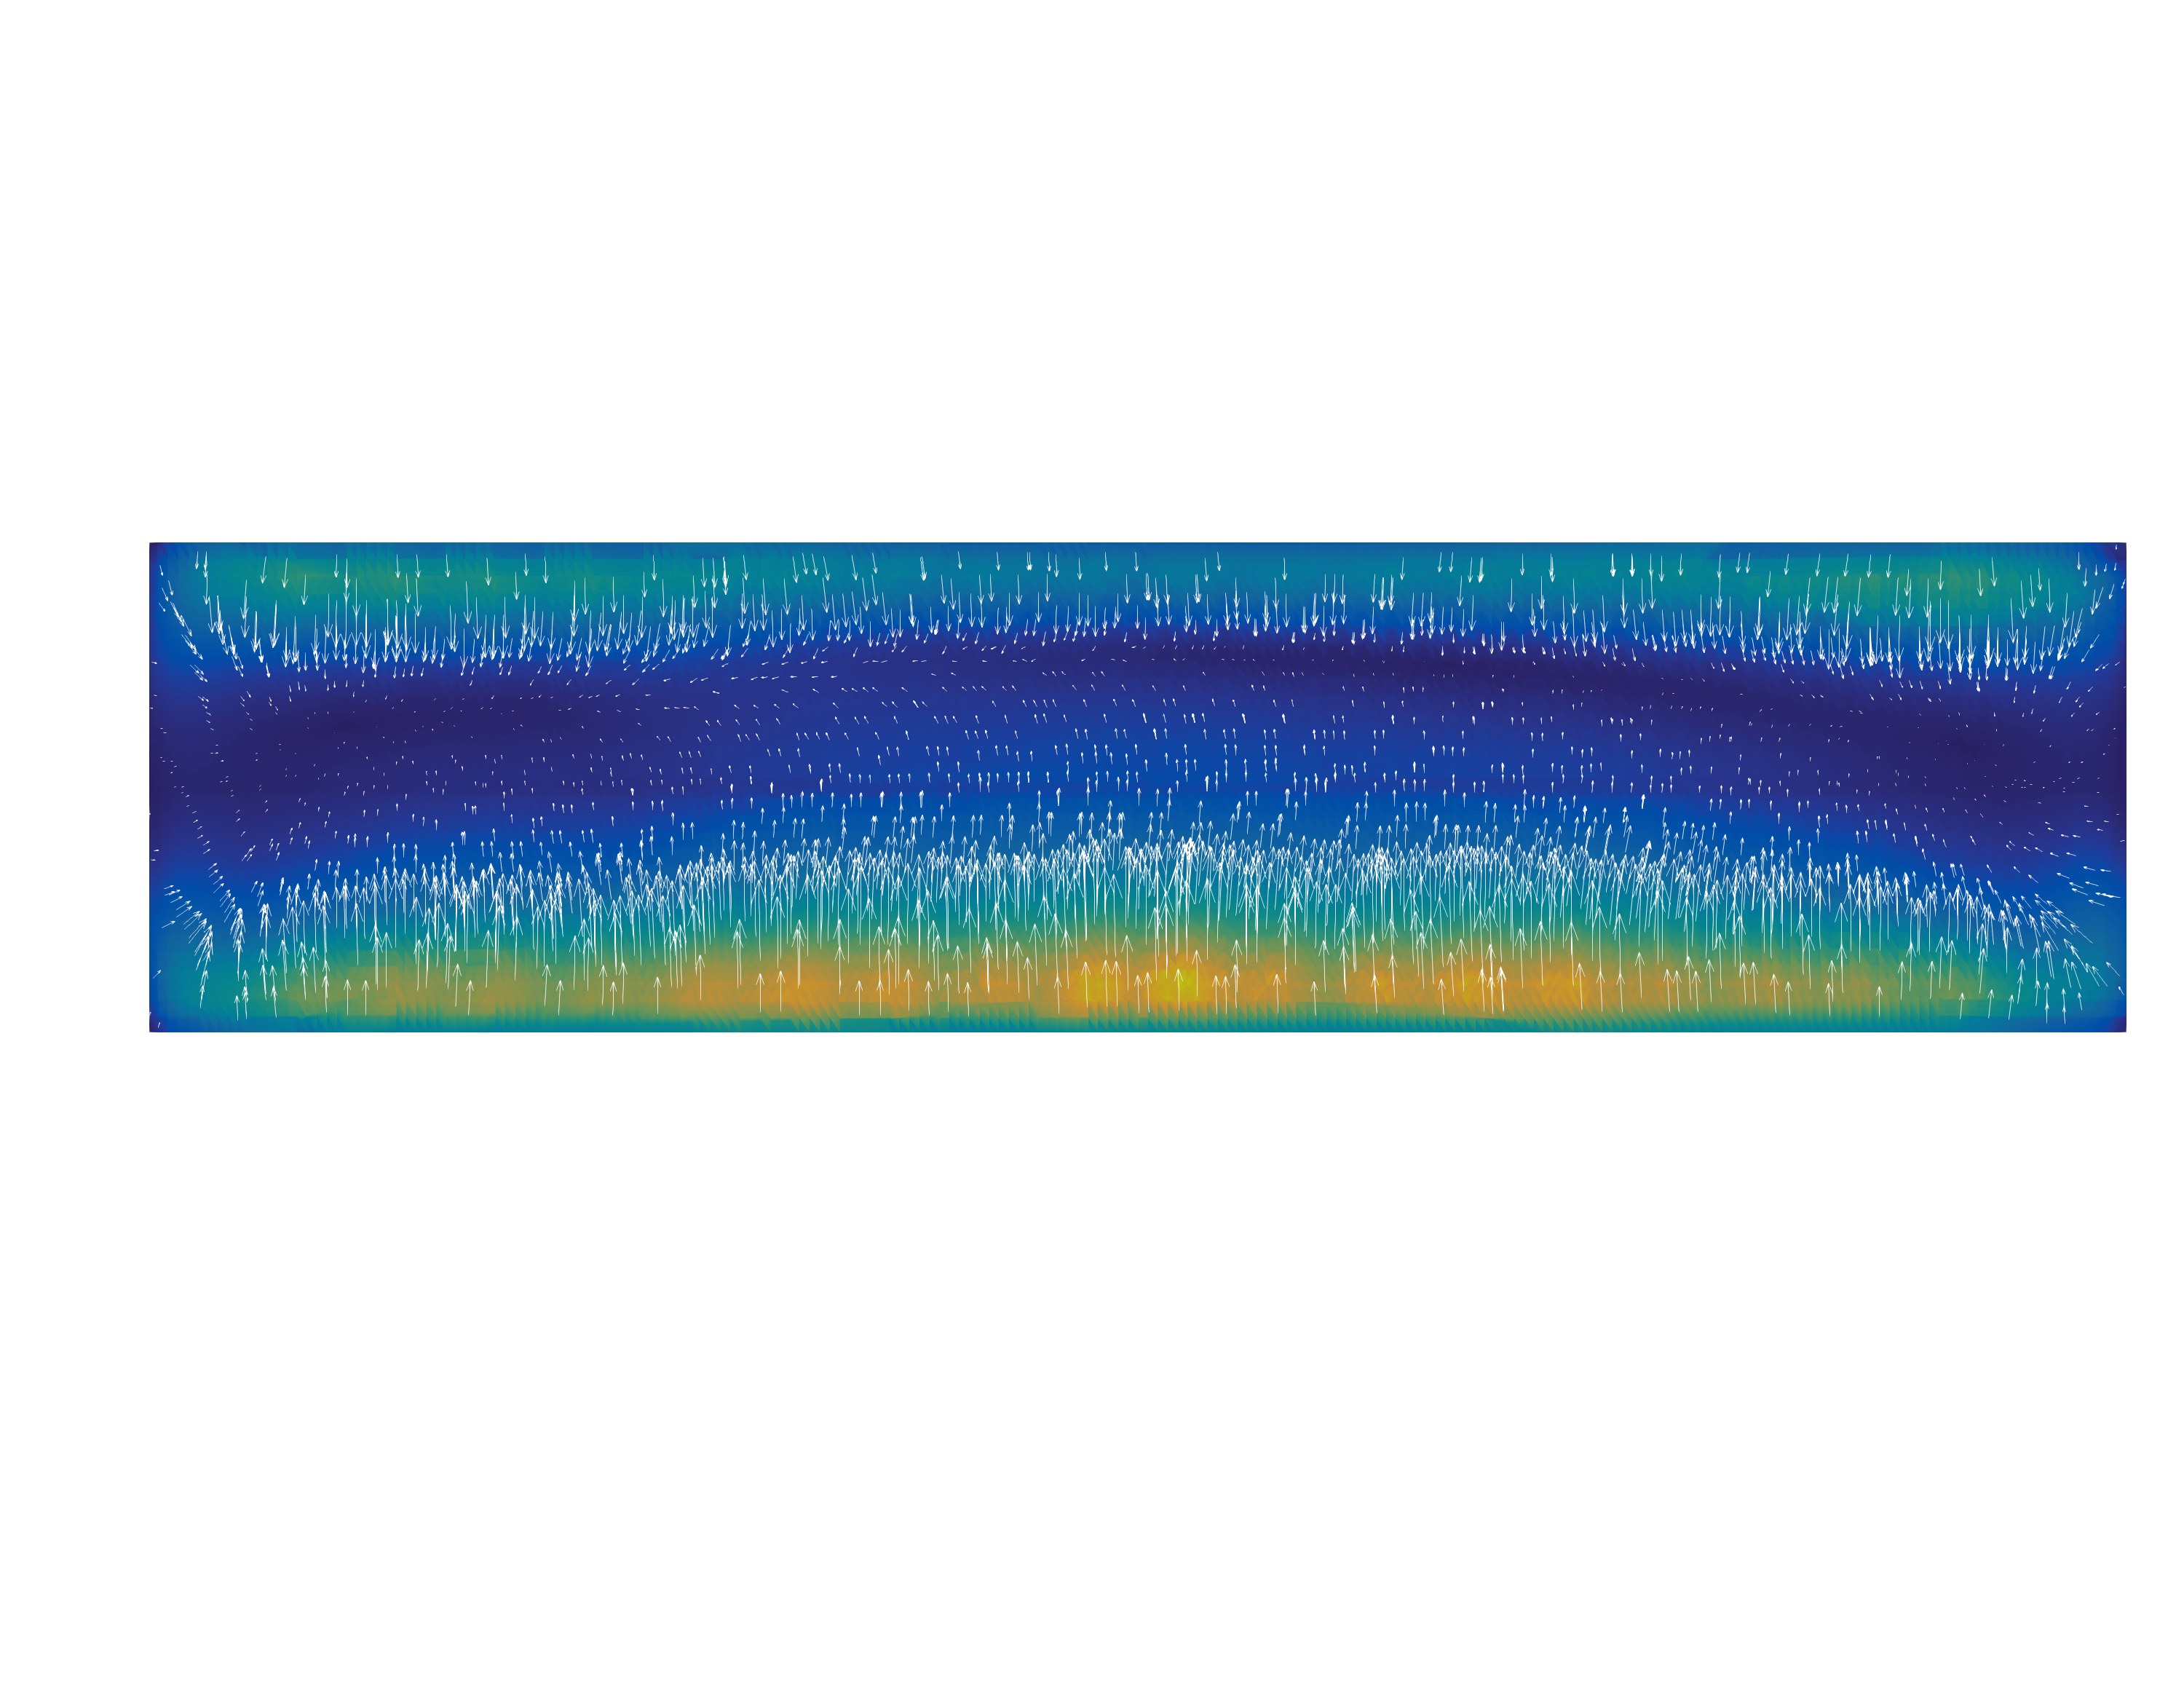
\includegraphics[width=\rasterimagewidth]{../media/fourier/application/print/force-h.png}};
      \end{axis}
    \end{tikzpicture}
    \caption{Champ de force $f$ dans le fluide issus du modèle 3D standard.}
    \label{fig:harmonic-force-h}
  \end{center}
\end{figure}

\begin{figure}[h!]
  \begin{center}
    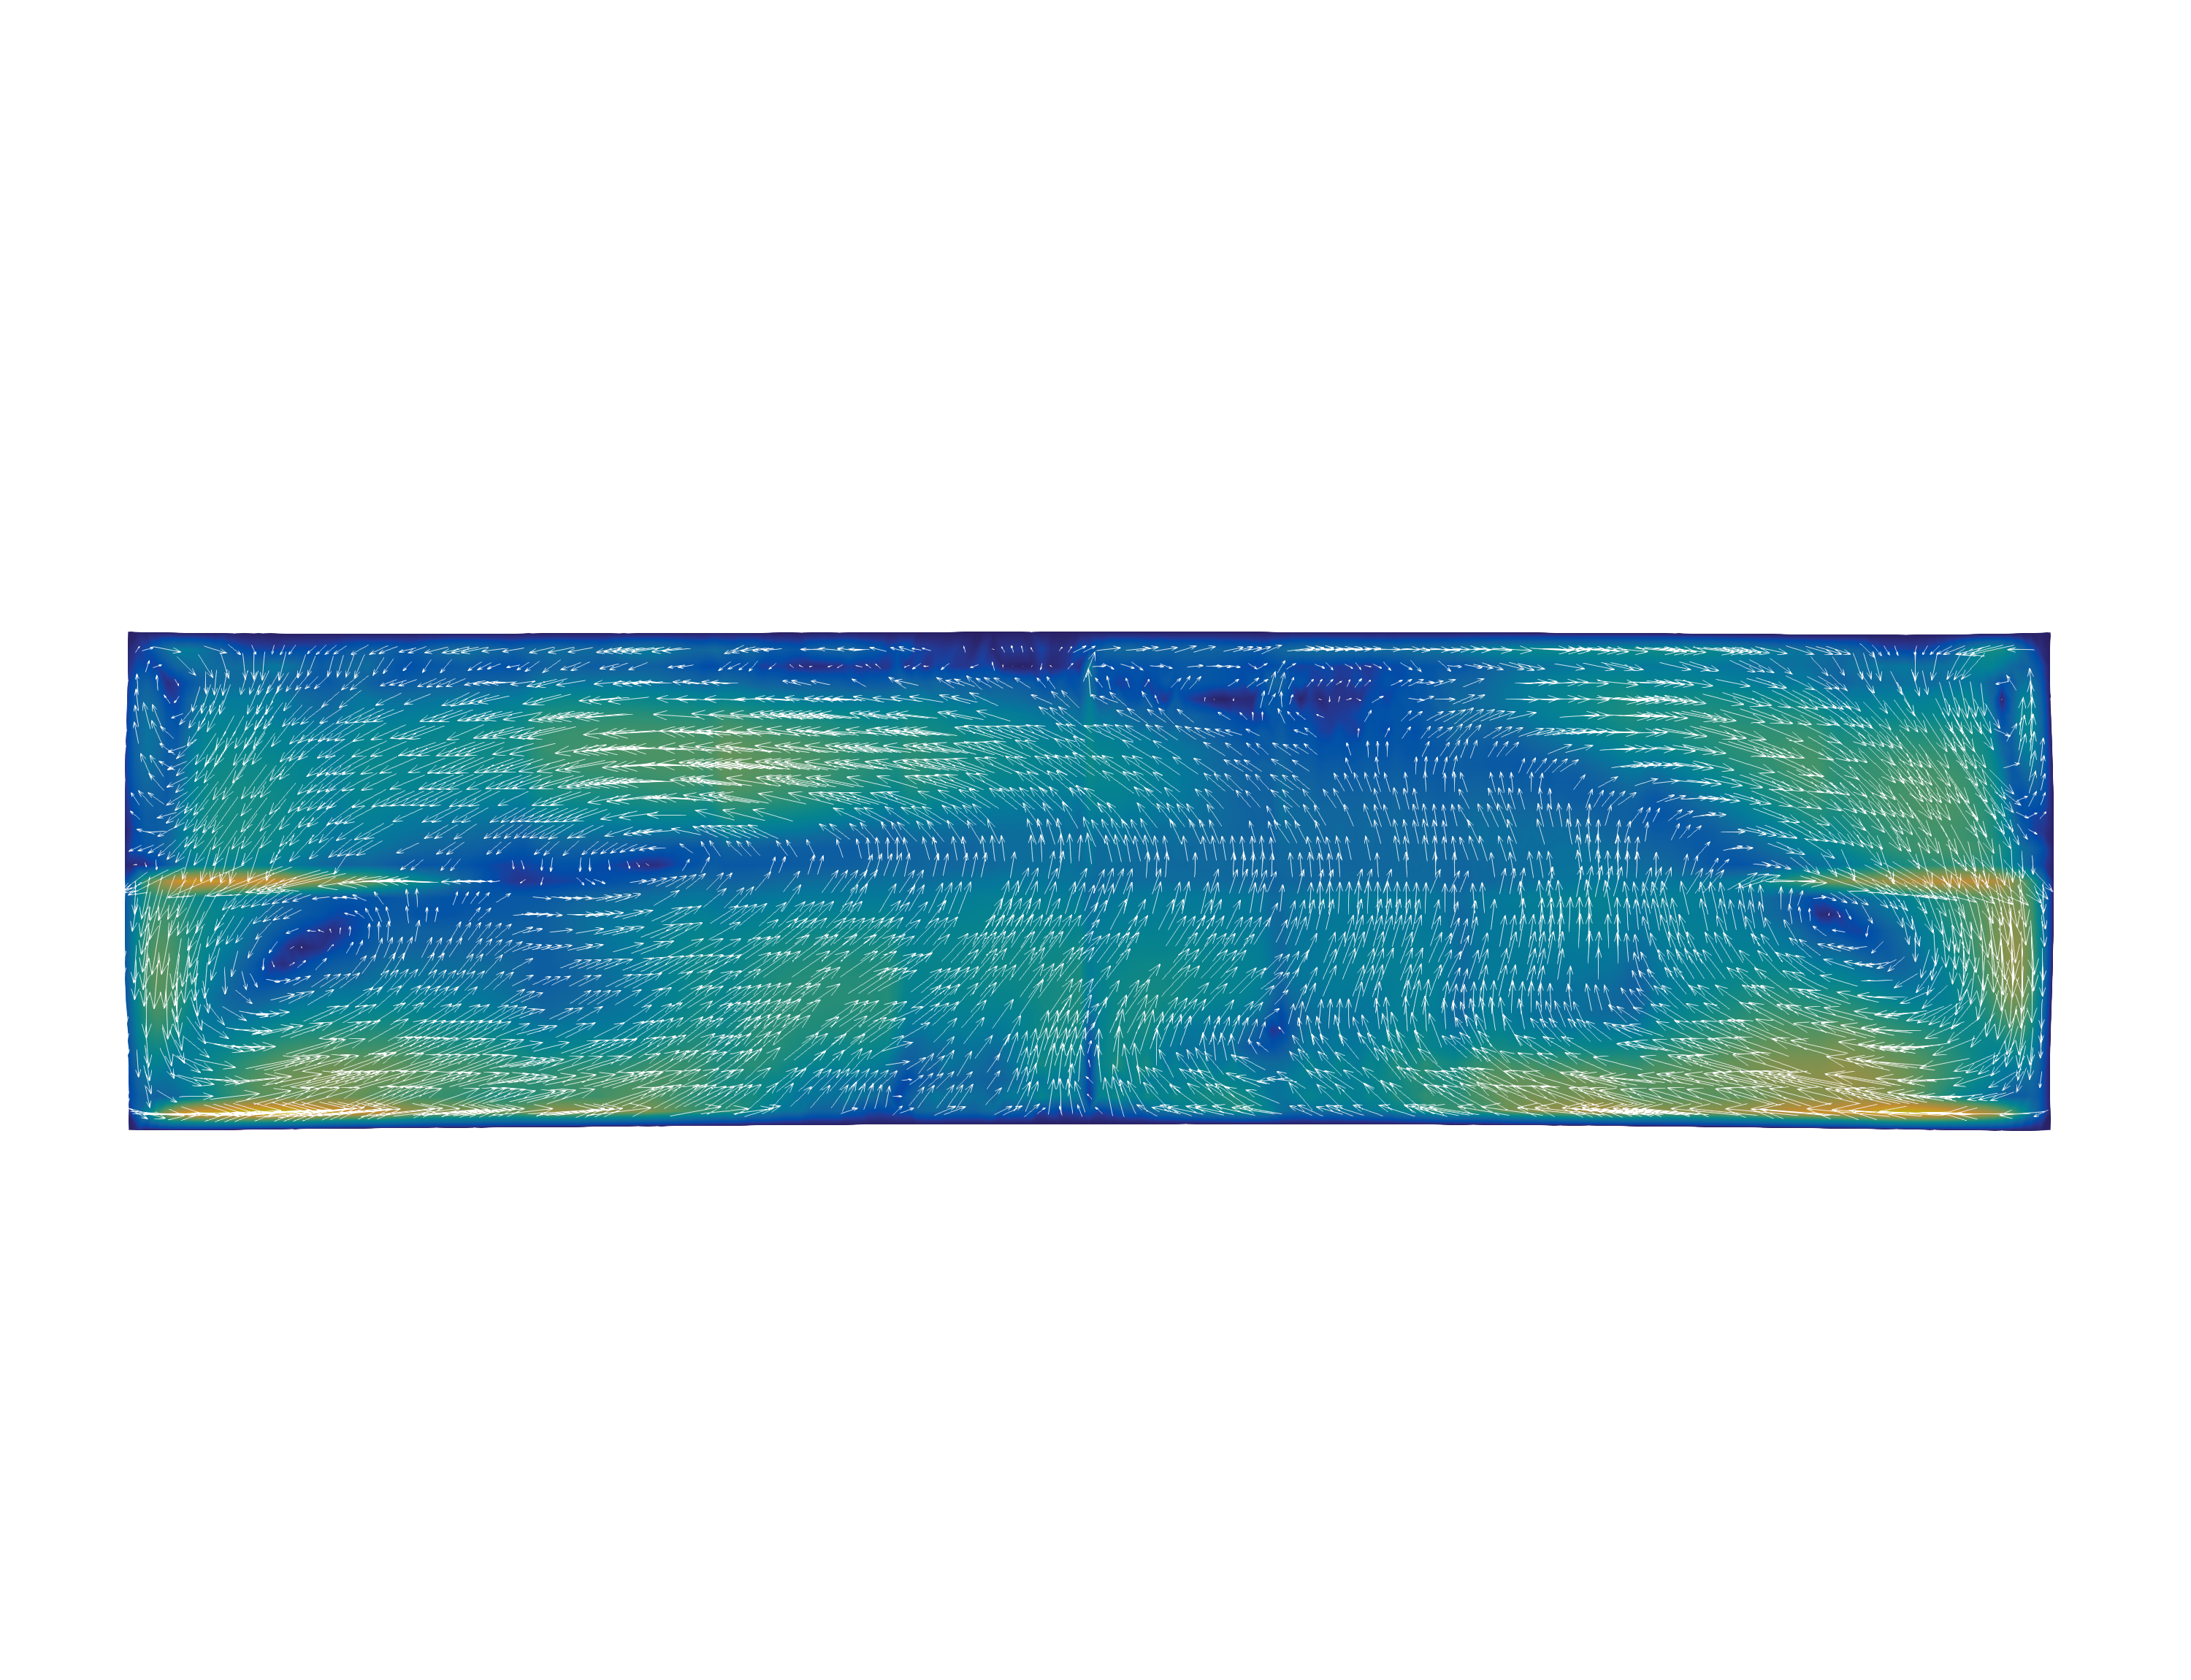
\includegraphics[width=\rasterimagewidth]{{../media/populations/ap32-fluid-flow/print/acd-all-anodes-velocity-0.00-0.05}.png}\\
    \begin{tikzpicture}
      \begin{axis}[
          colorbar,
          hide axis,
          scale only axis,
          height=0.41\rasterimagewidth,
          width=\rasterimagewidth,
          colorbar horizontal,
          point meta min=0.0,
          point meta max=6.0,
          colorbar style={
            title=Vitesse $u$ [\si{\centi\meter\per\second}],
            width=7.4cm,
            height=0.3cm,
            xtick={0.0, 3.0, 6.0},
            at={(0.5\rasterimagewidth,0.4cm)},
            anchor=north
          }
        ]
        \addplot [] coordinates {(0,0)};
        \node (myfirstpic) at (0,0) {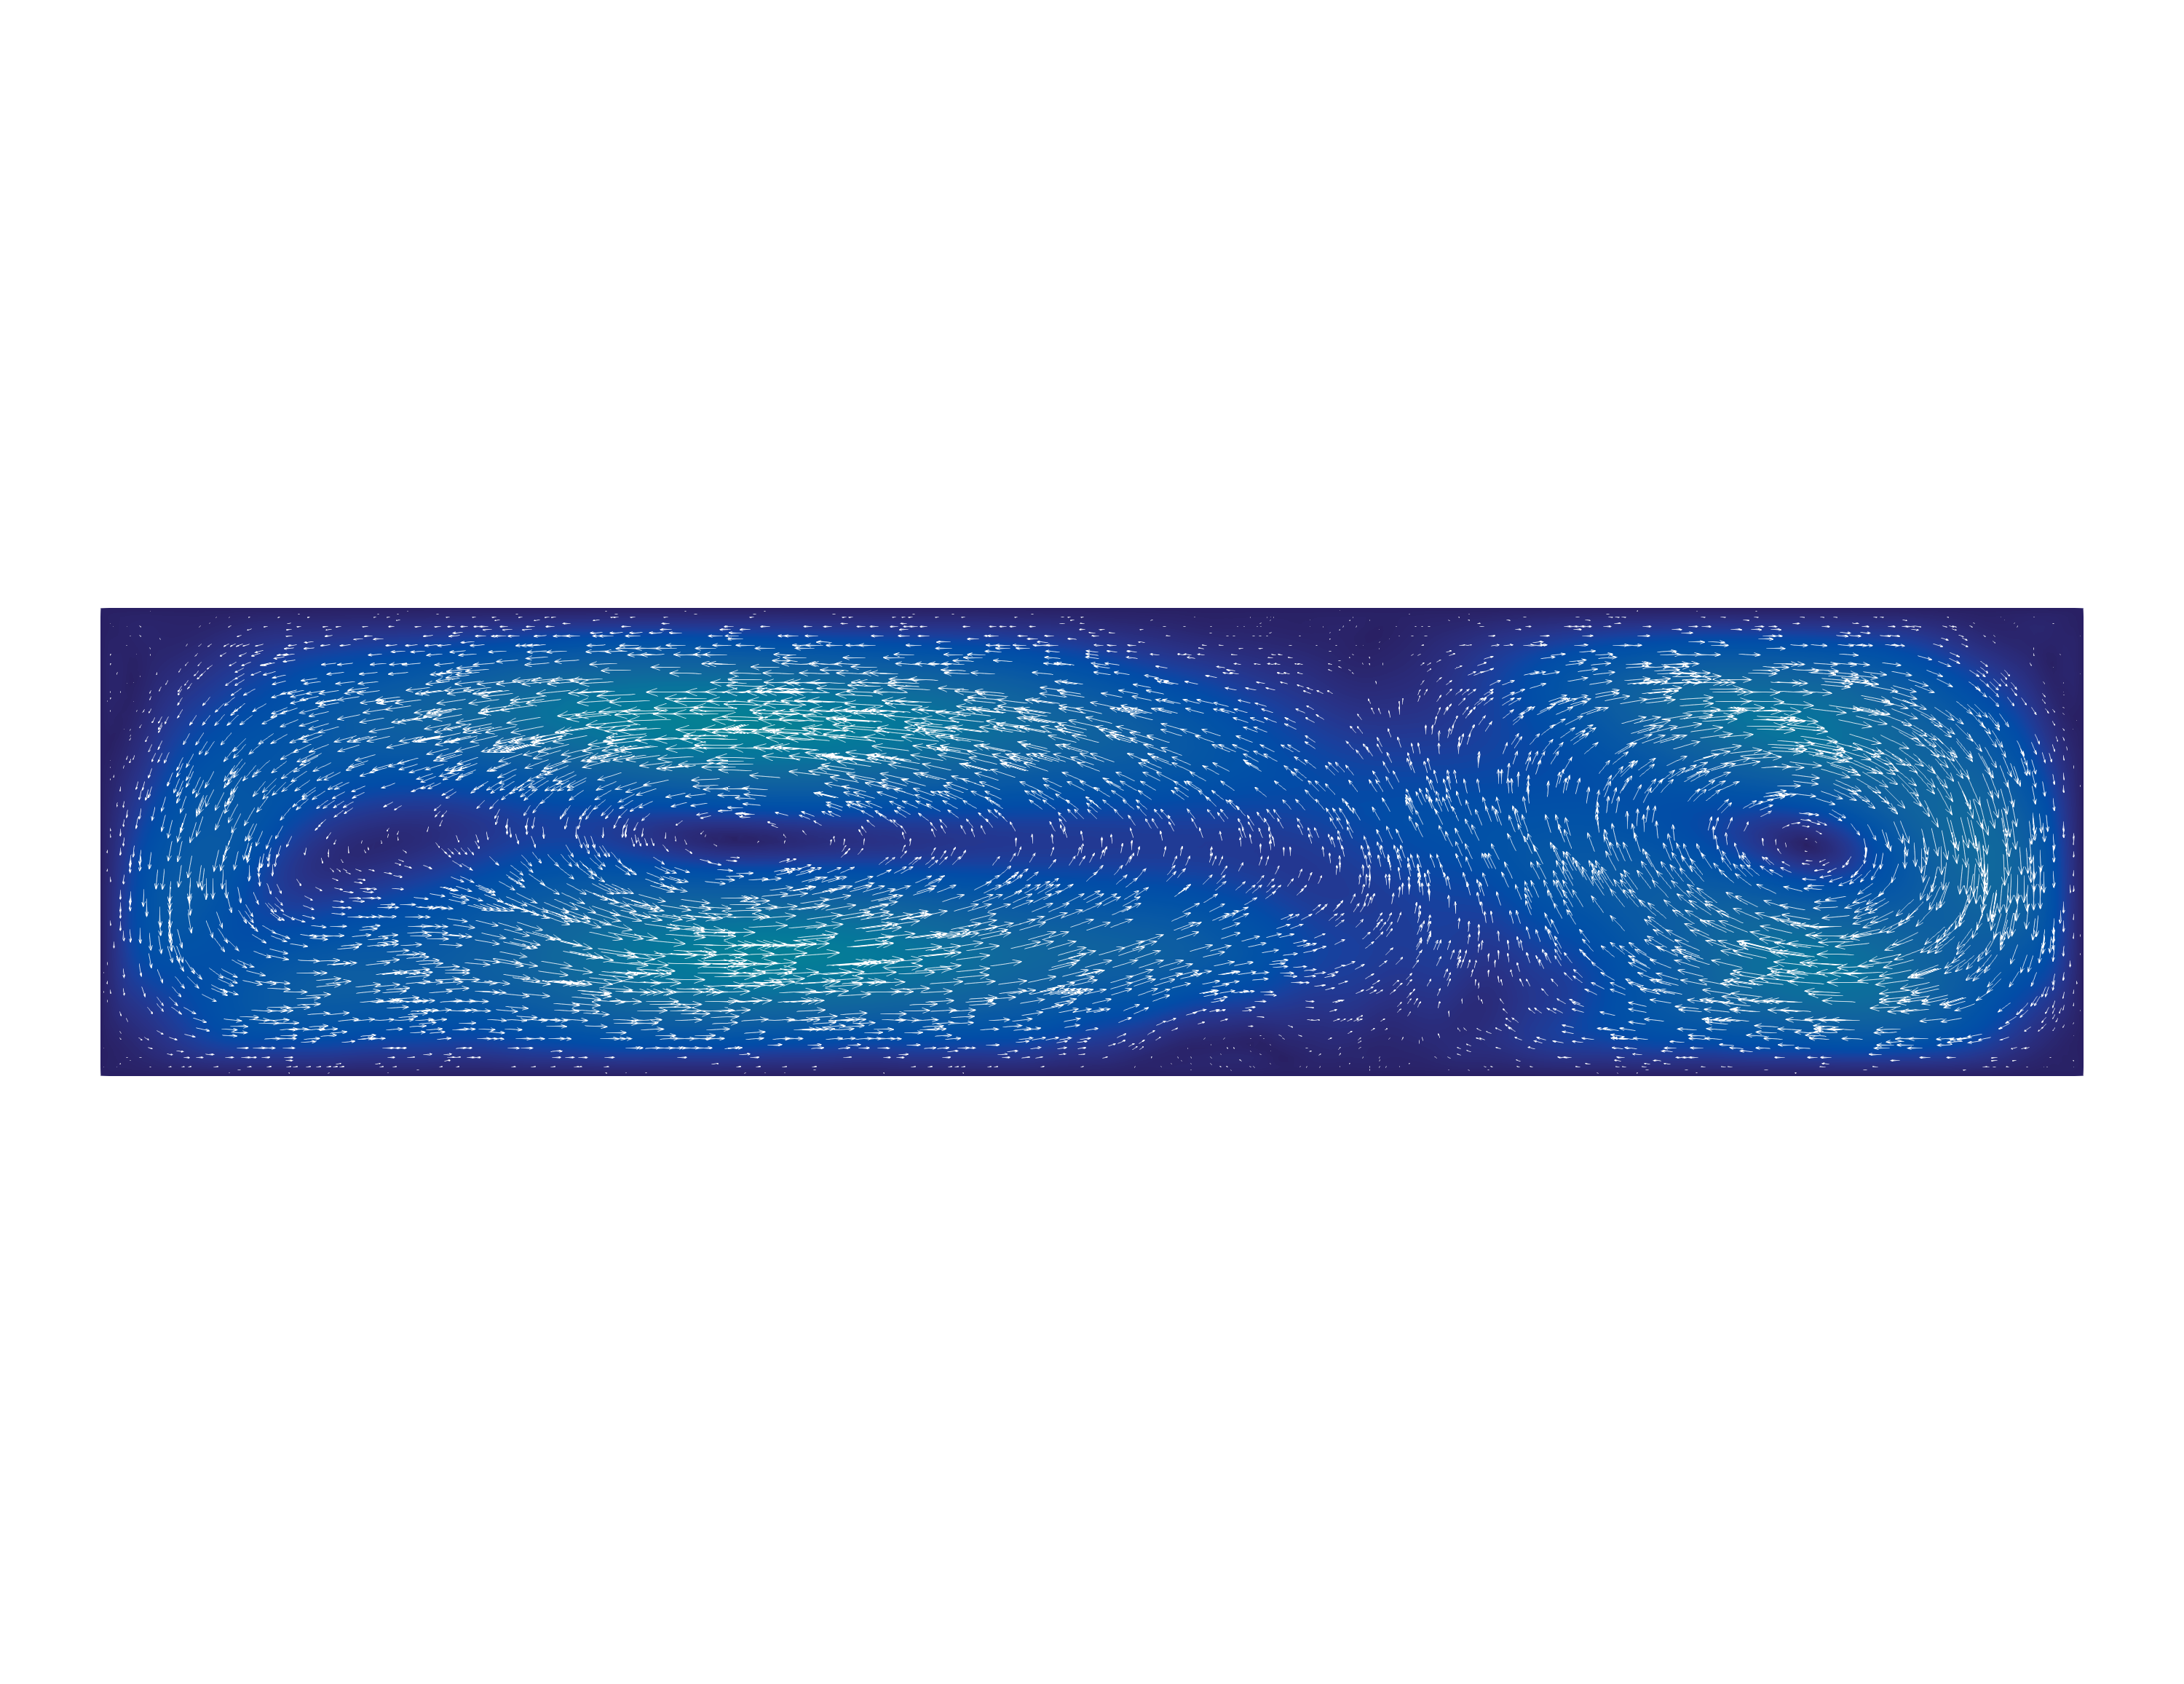
\includegraphics[width=\rasterimagewidth]{../media/fourier/application/print/all-velocity-harm.png}};
      \end{axis}
    \end{tikzpicture}
    \caption{Champ de vitesse stationnaire $u_h^{S3D}$ (haut) et
      $u_{h,K}^\mathrm{SF}$ reconstruit selon les équations
      (\ref{eq:u-h-12}), (\ref{eq:u-h-3}) (bas).}
    \label{fig:harmonic-velocity}
  \end{center}
\end{figure}

% conclusion:
%figure 4.6: \ref{fig:harmonic-velocity}
%figure 4.7: \ref{fig:harmonic-concentration}

On constate sur la figure \ref{fig:harmonic-velocity} que le champ de
courant $u_{h,K}^{\mathrm{SF}}$ reproduit les grandes structures de
l'écoulement $u_h^{\mathrm{S3D}}$: deux tourbillons principaux divise
la cuve, et la position de leur frontière correspond. Cependant, le
champ $u_{h,K}^{\mathrm{SF}}$ ne parvient pas a capturer les plus
petites structures qui apparaissent dans $u_h^{\mathrm{S3D}}$, soient
les petits tourbillons secondaires dans les coins en aval, ainsi
qu'une certaine asymétrie général par rapport à l'axe $x$.

\begin{figure}[h!]
  \begin{center}
    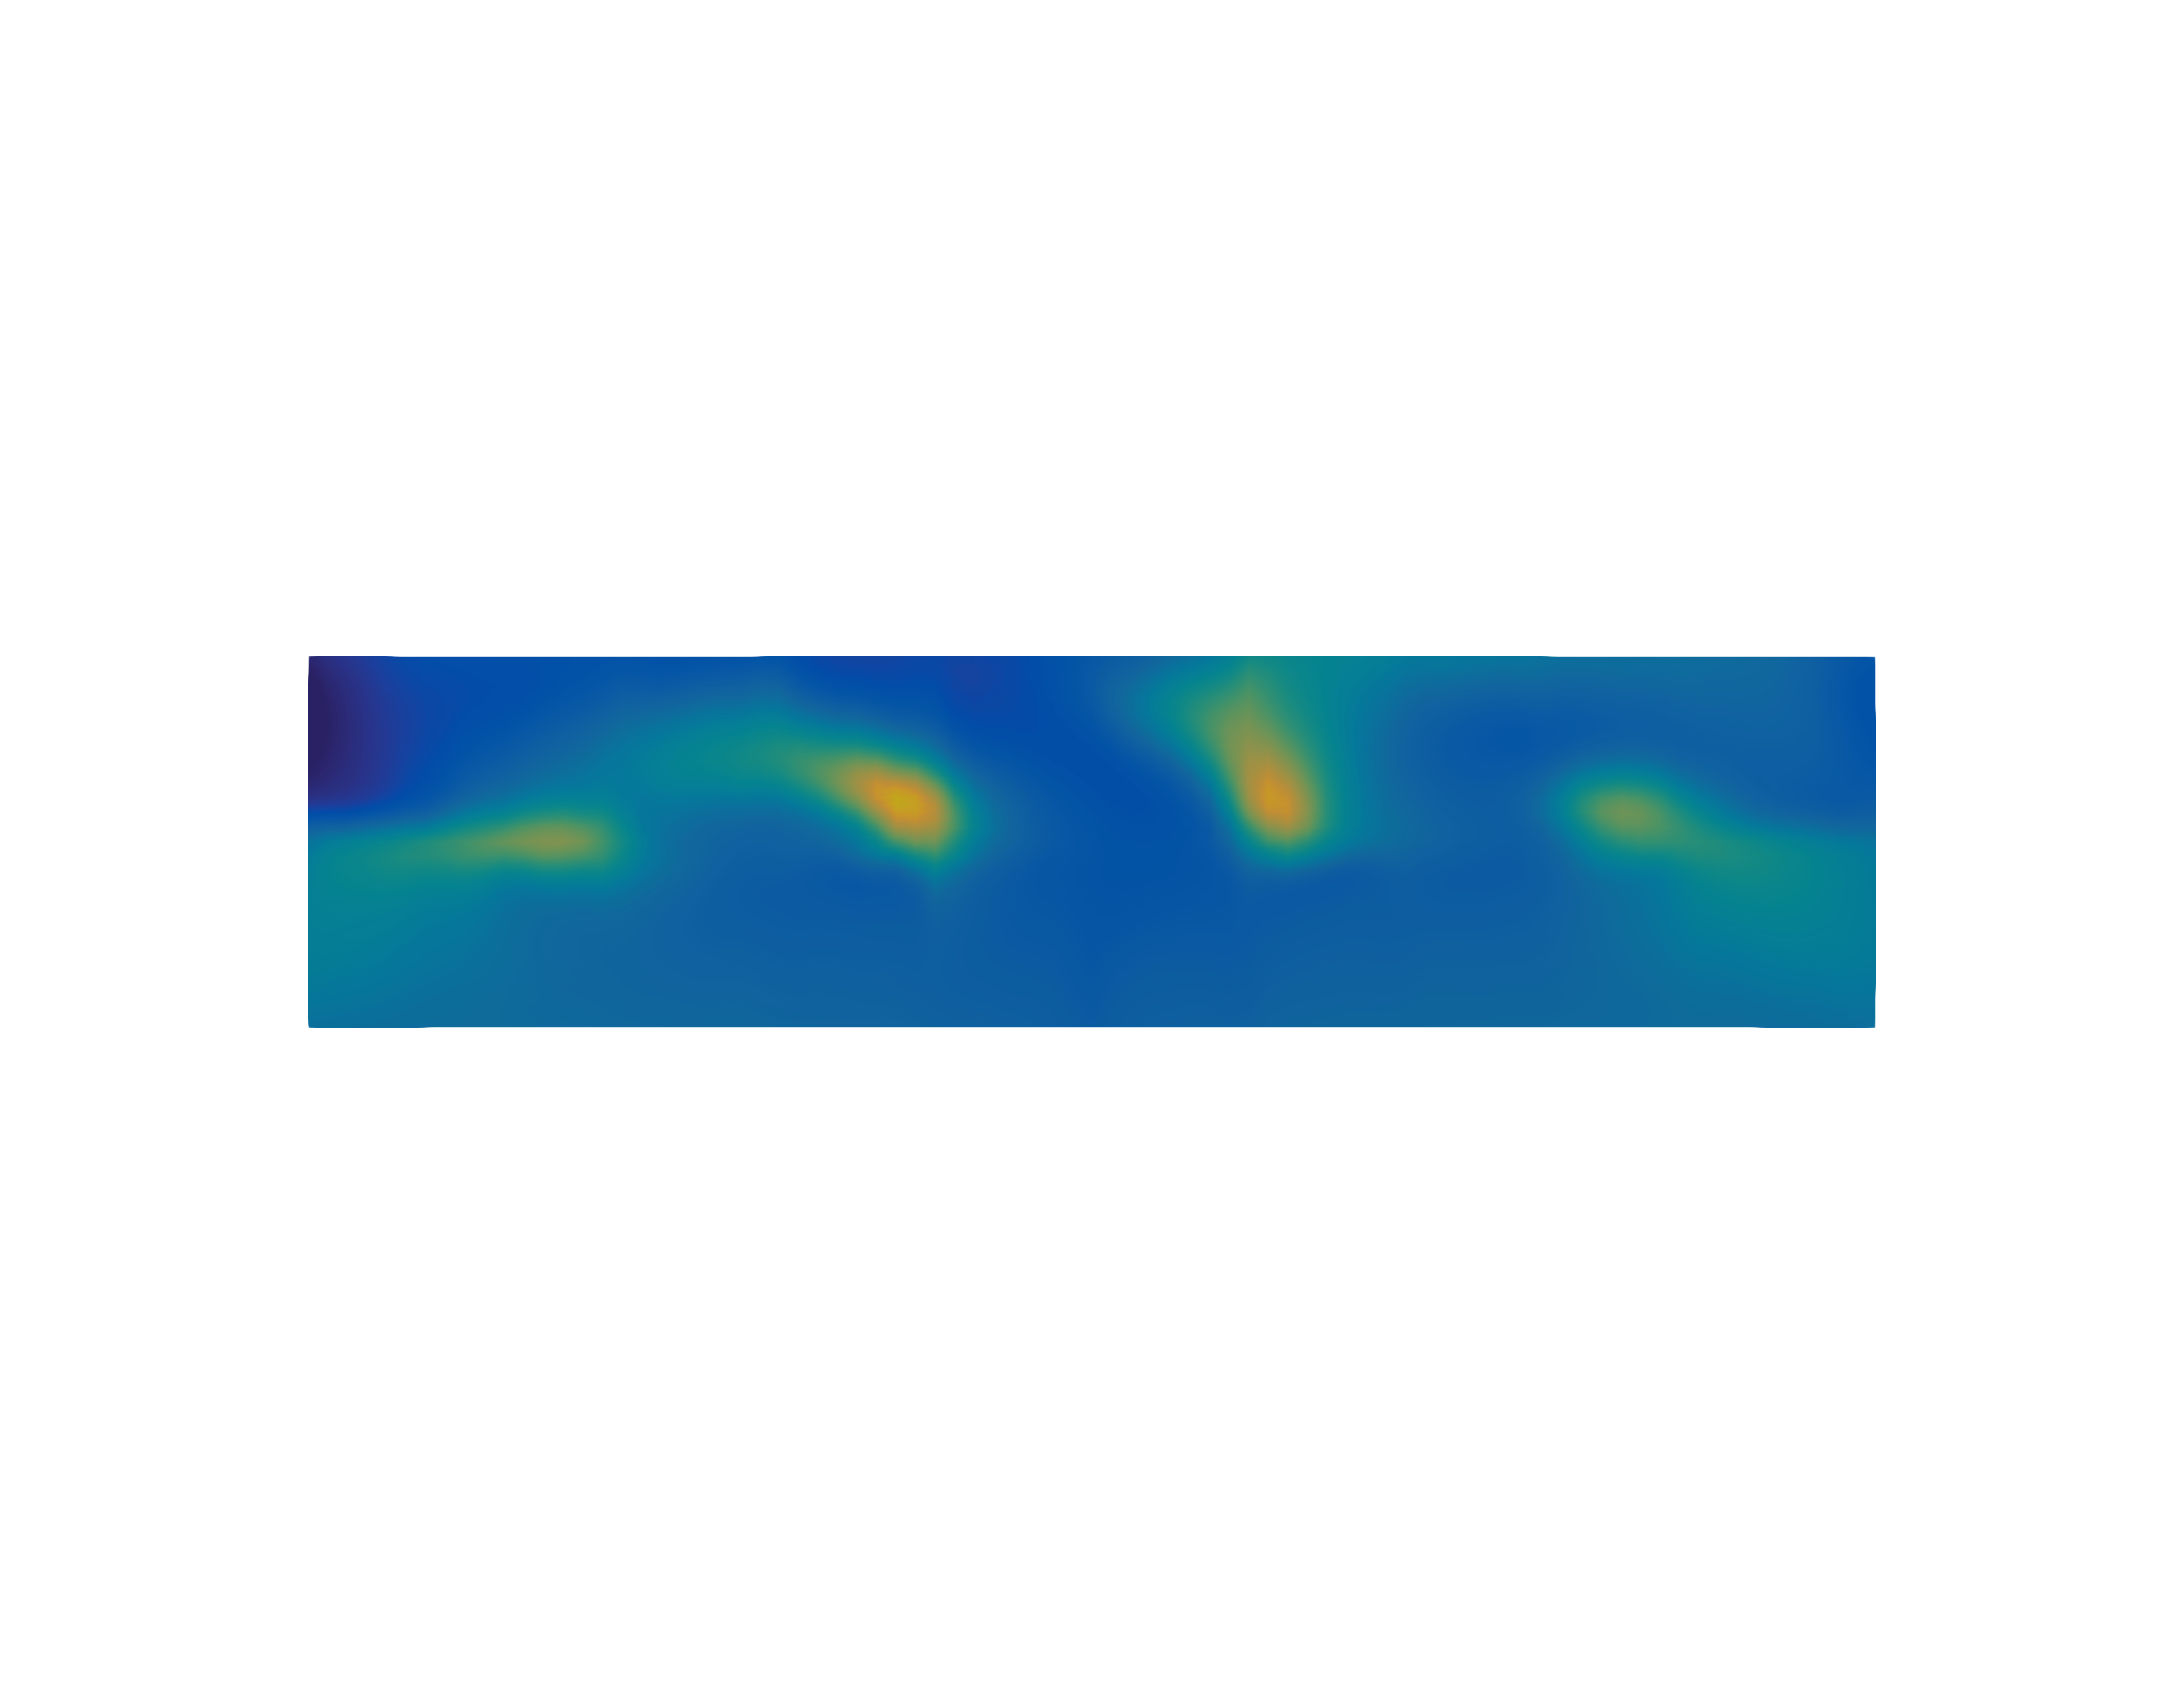
\includegraphics[width=\rasterimagewidth]{{../media/fourier/application/print/all-concentration-acd}.png}\\
    \begin{tikzpicture}
      \begin{axis}[
          colorbar,
          hide axis,
          scale only axis,
          height=0.41\rasterimagewidth,
          width=\rasterimagewidth,
          colorbar horizontal,
          point meta min=1.73,
          point meta max=6.84,
          colorbar style={
            title=Concentration $c$ [w\%],
            width=7.4cm,
            height=0.3cm,
            xtick={1.73, 3.0, 5.0, 6.84},
            at={(0.5\rasterimagewidth,0.4cm)},
            anchor=north
          }
        ]
        \addplot [] coordinates {(0,0)};
        \node (myfirstpic) at (0,0) {
          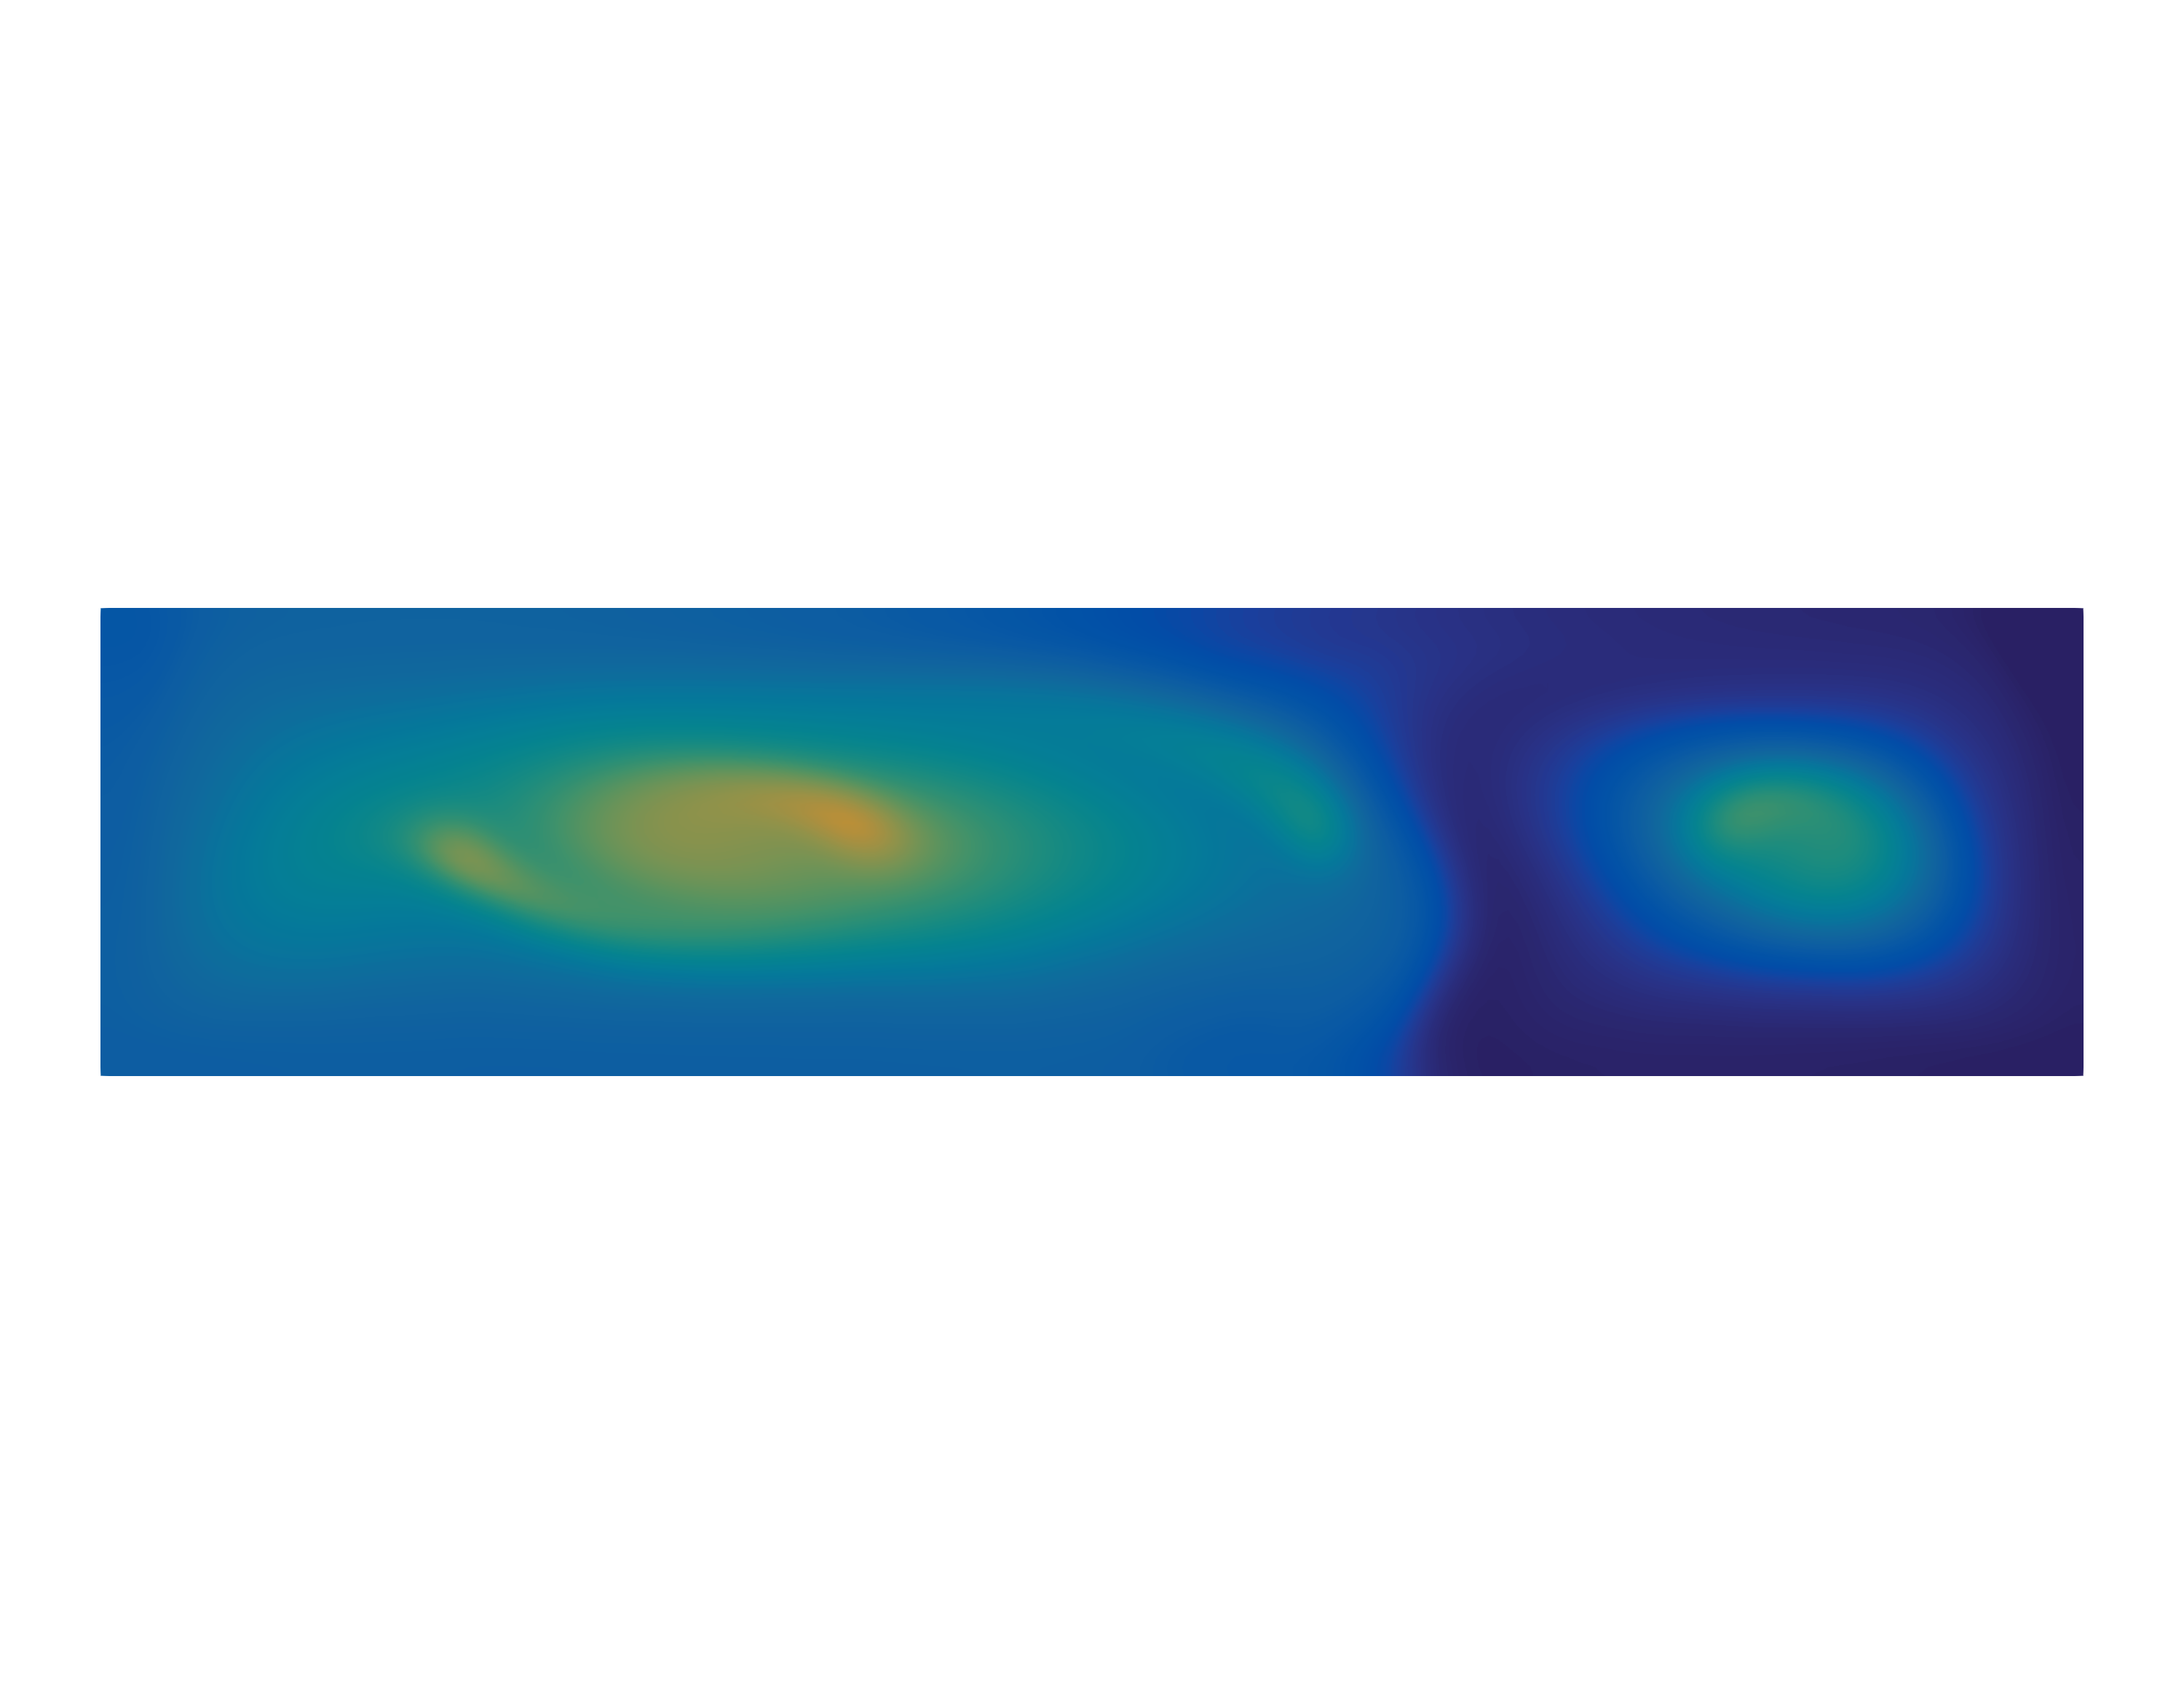
\includegraphics
              [width=\rasterimagewidth]
              {../media/fourier/application/print/all-concentration-harm.png}
        };
      \end{axis}
    \end{tikzpicture}
    \caption{Champ de concentration stationnaire $c_h^\mathrm{S3D}$
      (haut) et $c_{h}^\mathrm{SF}$
      solution de l'équation (\ref{eq:stat-concentration}) (bas).}
    \label{fig:harmonic-concentration}
  \end{center}
\end{figure}

En comparaison avec le champ $c_h^\mathrm{S3D}$ (en
haut sur la figure \ref{fig:harmonic-concentration}), le champ de
concentration stationnaire $c_h^\mathrm{SF}$ (en bas sur la
figure \ref{fig:harmonic-concentration}) reproduit certains aspects
caractéristiques. En particulier, les amplitudes de variation de la
concentration sont très similaires. De plus, la position des points
d'injections apparaît clairement dans sur les deux calculs. En
revanche, le champ $c_h^\mathrm{SF}$ présente une zone appauvrie en
périphérie du tourbillon de droite, qui n'est pas présente dans
le champ $c_h^\mathrm{S3D}$.

\subsection{Désactivation d'anodes}
On s'intéresse maintenant au cas du calcul de l'écoulement des fluides
et de la concentration d'alumine dissoute dans le bain électrolytique
lorsqu'on désactive une anode, c'est-à-dire que l'une des anodes du
plan anodique n'est pas conductrice électriquement. Cette situation a
lieu en pratique lorsqu'une anode en fin de vie est remplacée par une
anode neuve, mais froide. Sa conductivité électrique qui est
quasi-nulle initialement, augmente au fur et à mesure que l'anode
atteint sa température d'opération. Dans cette partie, on dénotera
conjointement la vitesse du fluide stationnaire et la concentration
d'alumine dissoute obtenue qui résultent du modèle décrit dans le
chapitre \ref{chap:populations} par l'abréviation S3D. Dans cette
partie, on considérera uniquement une dissolution des particules
d'alumine indépendante de la température, c'est-à-dire que le champ
$c^\mathrm{S3D}$ est calculé avec le modèle standard 3D (S3D) en désactivant
la dépendance de la vitesse de dissolution en fonction de la
température du bain.

Dans le modèle S3D, on peut simuler la désactivation d'une anode en
annulant la conductivité électrique $\conductivity$ dans le volume
occupé par ladite anode. On a donc la densité de courant $j =
\conductivity\parent{\nabla \phi + u^\mathrm{S3D}}$, $\div j = 0$, où
$\phi$ est le potentiel électrique, $u^\mathrm{S3D}$ l'écoulement des
fluides solution des équations de Navier-Stokes, $B$ le champ
d'induction magnétique solution des équations de Maxwell et la force
$f = j\times B$. Dans le modèle SF, on utilise le champ de force $f$
issus d'un calcul S3D avec toutes les anodes activées, restreint à
$\Omega$. On simule la désactivation d'une anode en supposant que la
densité de courant électrique est quasiment nulle sous celle-ci, ce
qui revient à imposer $f = 0$ sous l'anode désactivée (voir figure
\ref{fig:anode-deactivation}). L'emplacement des anodes vues depuis
dessus et leur numérotation dans la cuve AP32 est schématisé sur la
figure \ref{fig:anode-numerotations}.

Les figures \ref{fig:f3d-deactivated-a}, \ref{fig:f3d-deactivated-b},
présente le champ de vitesse stationnaire $u^{S3D}$ du bain
électrolytique dans l'ACD de la cuve AP32 et la distribution de
concentration $c^{S3D}$, pour quatre configurations différentes du
plan anodique, soit les anodes $(1,1)$, $(1,2)$, $(2,1)$ et $(2,2)$
successivement désactivées. On se réfère à la figure
\ref{fig:anode-numerotations} pour le placement de chacune de ces
anodes. Les anodes désactivées se trouvent au niveau de l'extrémité
gauche de la cuve. On note que l'influence sur le champ de vitesse et
la distribution de concentration s'étend à proximité de l'anode
désactivée, mais ne s'étend pas à l'ensemble de la cuve.

\begin{figure}[h!]
  \begin{center}
    \input{../media/fourier/anode-deactivation/anode-deactivation.pdf_tex}
    \caption{Désactivation d'une anode dans le modèle standard S3D et
      le modèle SF. (a) Dans le modèle S3D, la désactivation d'une
      anode est modélisée par l'annulation de sa conductivité
      électrique $\conductivity$. (b.1) Calcul du terme de force avec
      le modèle S3D et toutes les anodes activées. (b.2) Calcul de
      l'écoulement dans le domaine $\Omega$ avec le modèle SF et la
      force obtenue en (b.1), mais annulée sous l'anode désactivée.}
    \label{fig:anode-deactivation}
  \end{center}
\end{figure}


% figures 4.12, 4.13
Pour évaluer l'effet des approximations introduites par le modèle
SF par rapport au modèle S3D, on compare les champs de vitesse
$u_h^{\mathrm{S3D}}$ et $u_h^{\mathrm{SF}}$. Pour le calcul de
$u_h^{\mathrm{SF}}$, on utilise le champ de force $f$ issus du calcul de
$u_h^{\mathrm{S3D}}$. Sur les figures \ref{fig:harmonic-velocity-comp-a}, \ref{fig:harmonic-velocity-comp-b}
on peut comparer les champs de vitesse $u_h^{\mathrm{S3D}}$ et
$u_h^\mathrm{SF}$ sur une surface horizontale placée respectivement
dans l'ACD de la cuve AP32 ou dans le domaine $\Omega$ à une hauteur
correspondante.


%figure 4.14, 4.15
L'objectif final est de calculer le champ de concentration d'alumine
dans le bain électrolytique. Sur les figures
\ref{fig:harmonic-concentration-comp-a},
\ref{fig:harmonic-concentration-comp-b}, on compare les champs de
concentration $c^\mathrm{S3D}$ et le champ de concentration
stationnaire $c^\mathrm{SF}$ dans le domaine $\Omega$ avec le modèle
SF. On obtient le champ de transport $u_h^\mathrm{SF}$ qui sert au
calcul de $c_h^\mathrm{SF}$ en utilisant le champ de force $f$ issus
du calcul de $u^\mathrm{S3D}$ avec l'anode correspondante désactivée
(voir figure \ref{fig:anode-deactivation}a).

\begin{figure}[h!]
  \begin{center}
    \input{../media/fourier/anode-numerotations/anode-numerotation.pdf_tex}
    \caption{Numérotation des anodes de la cuve AP32.}
    \label{fig:anode-numerotations}
  \end{center}
\end{figure}

L'objectif du modèle étant d'obtenir une approximation du champ de
vitesse et du champ de concentration à moindre coût, on veut éviter à
tout prix de devoir utiliser le modèle S3D pour obtenir le champ de
force en fonction de la configuration du plan anodique. A la place, on
effectue un calcul de la force que l'on note $f^0$ avec le modèle S3D
dans la configuration où toutes les anodes sont actives (voir figure
\ref{fig:anode-deactivation}b.1 et
\ref{fig:anode-deactivation}b.2). La force $f^0$ est représentée sur
la figure \ref{fig:harmonic-force-h}.

\begin{figure}[!h]
  \begin{center}
    \begin{subfigure}[t]{\textwidth}
      \begin{center}
        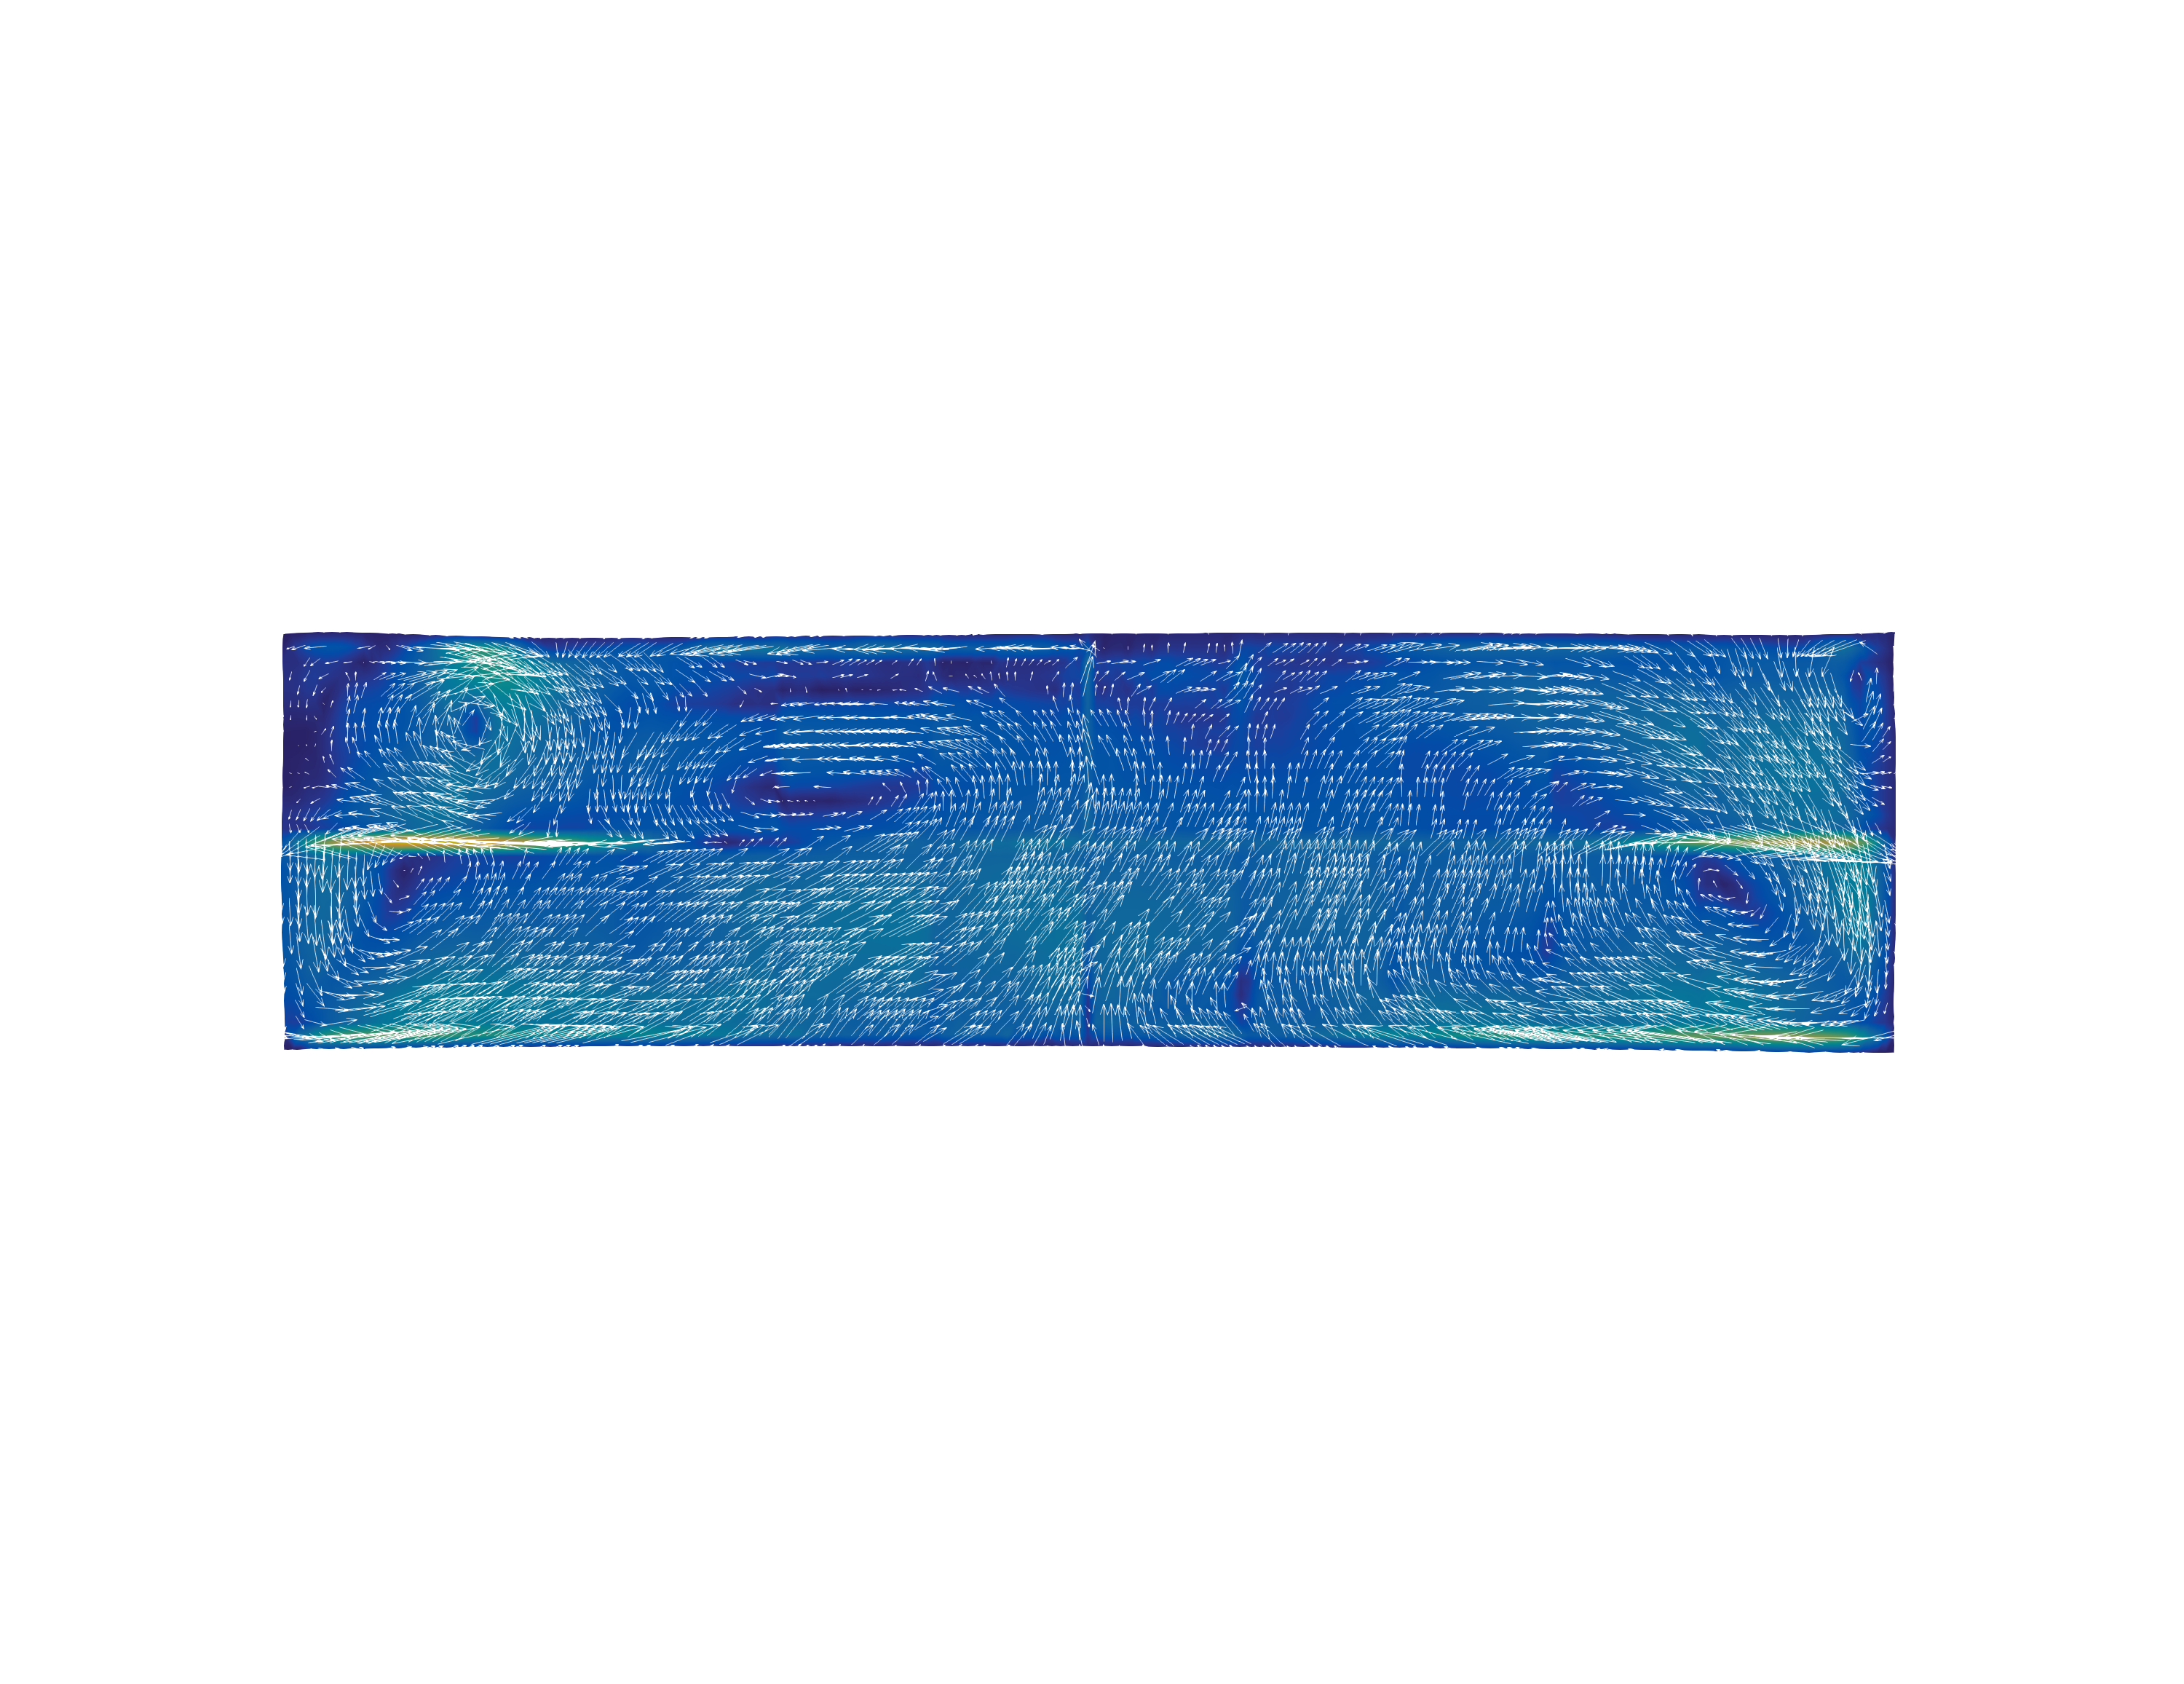
\includegraphics[width=0.9\textwidth]{../media/fourier/application/print/ab-0-1-velocity-acd.png}
        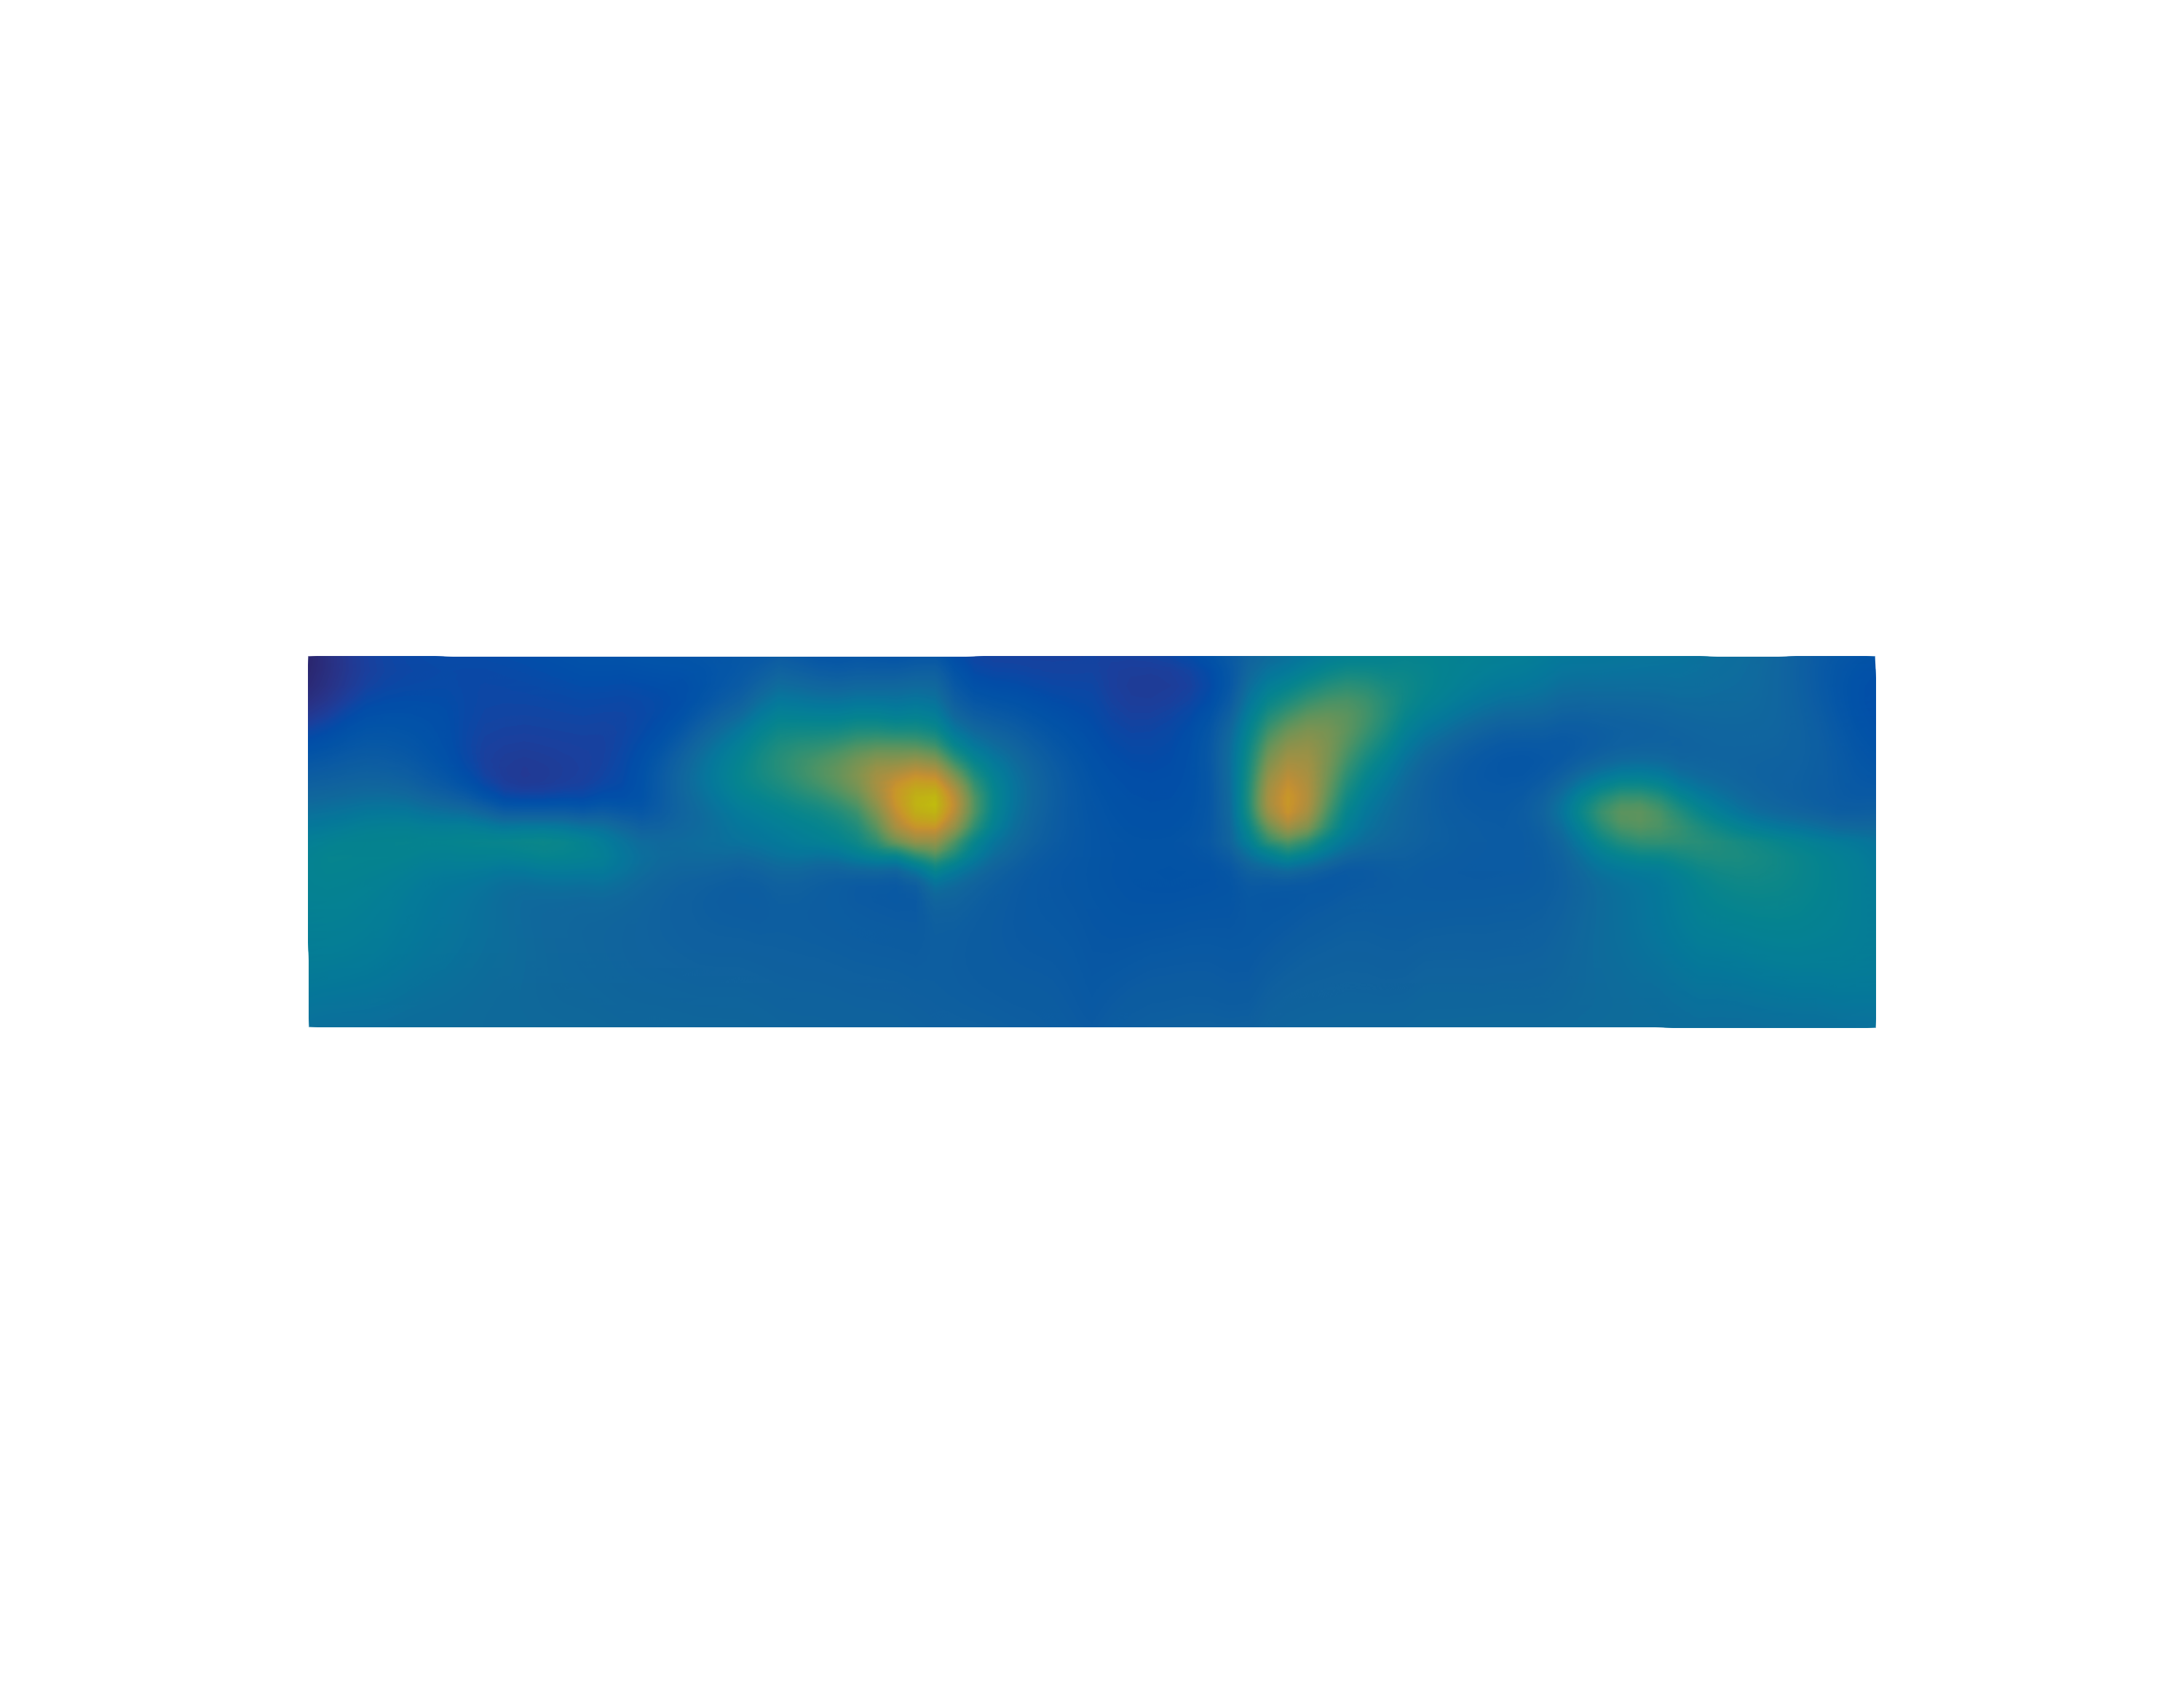
\includegraphics[width=0.9\textwidth]{../media/fourier/application/print/ab-0-1-concentration-acd.png}
        \caption{Anode $(1,1)$ désactivée}
      \end{center}
    \end{subfigure}
    \begin{subfigure}[t]{\textwidth}
      \begin{center}
        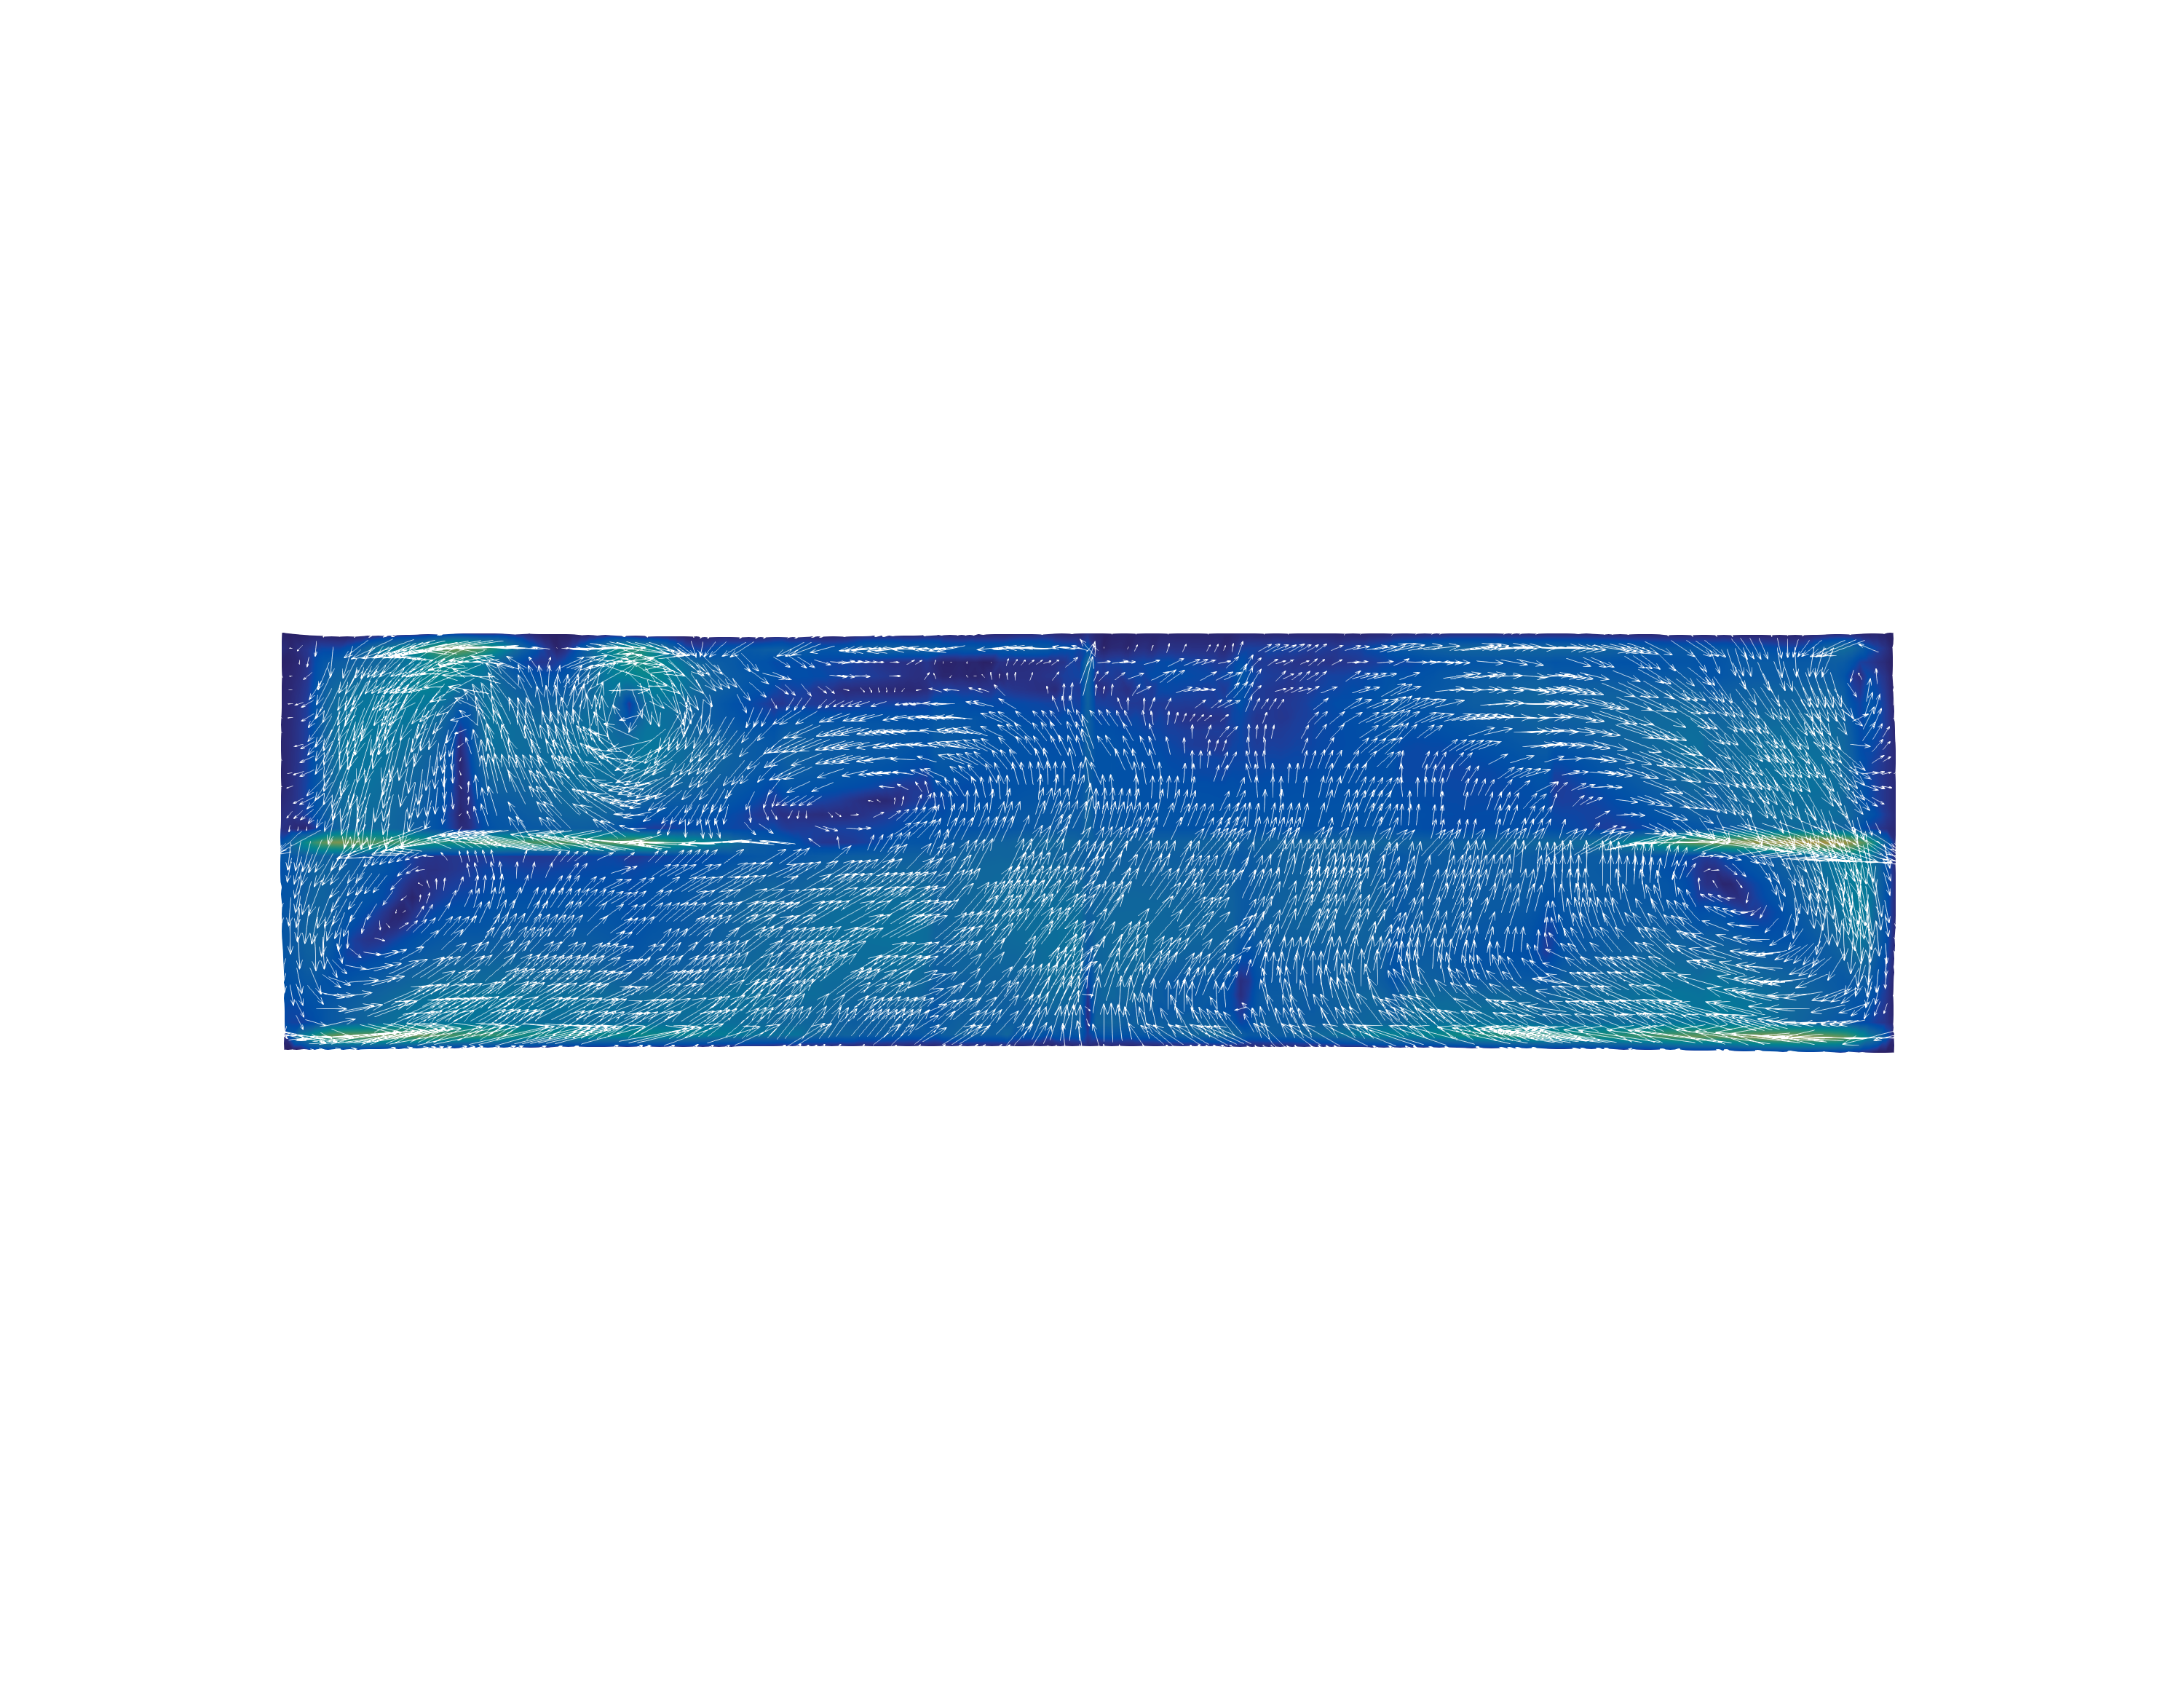
\includegraphics[width=0.9\textwidth]{../media/fourier/application/print/ab-0-2-velocity-acd.png}
        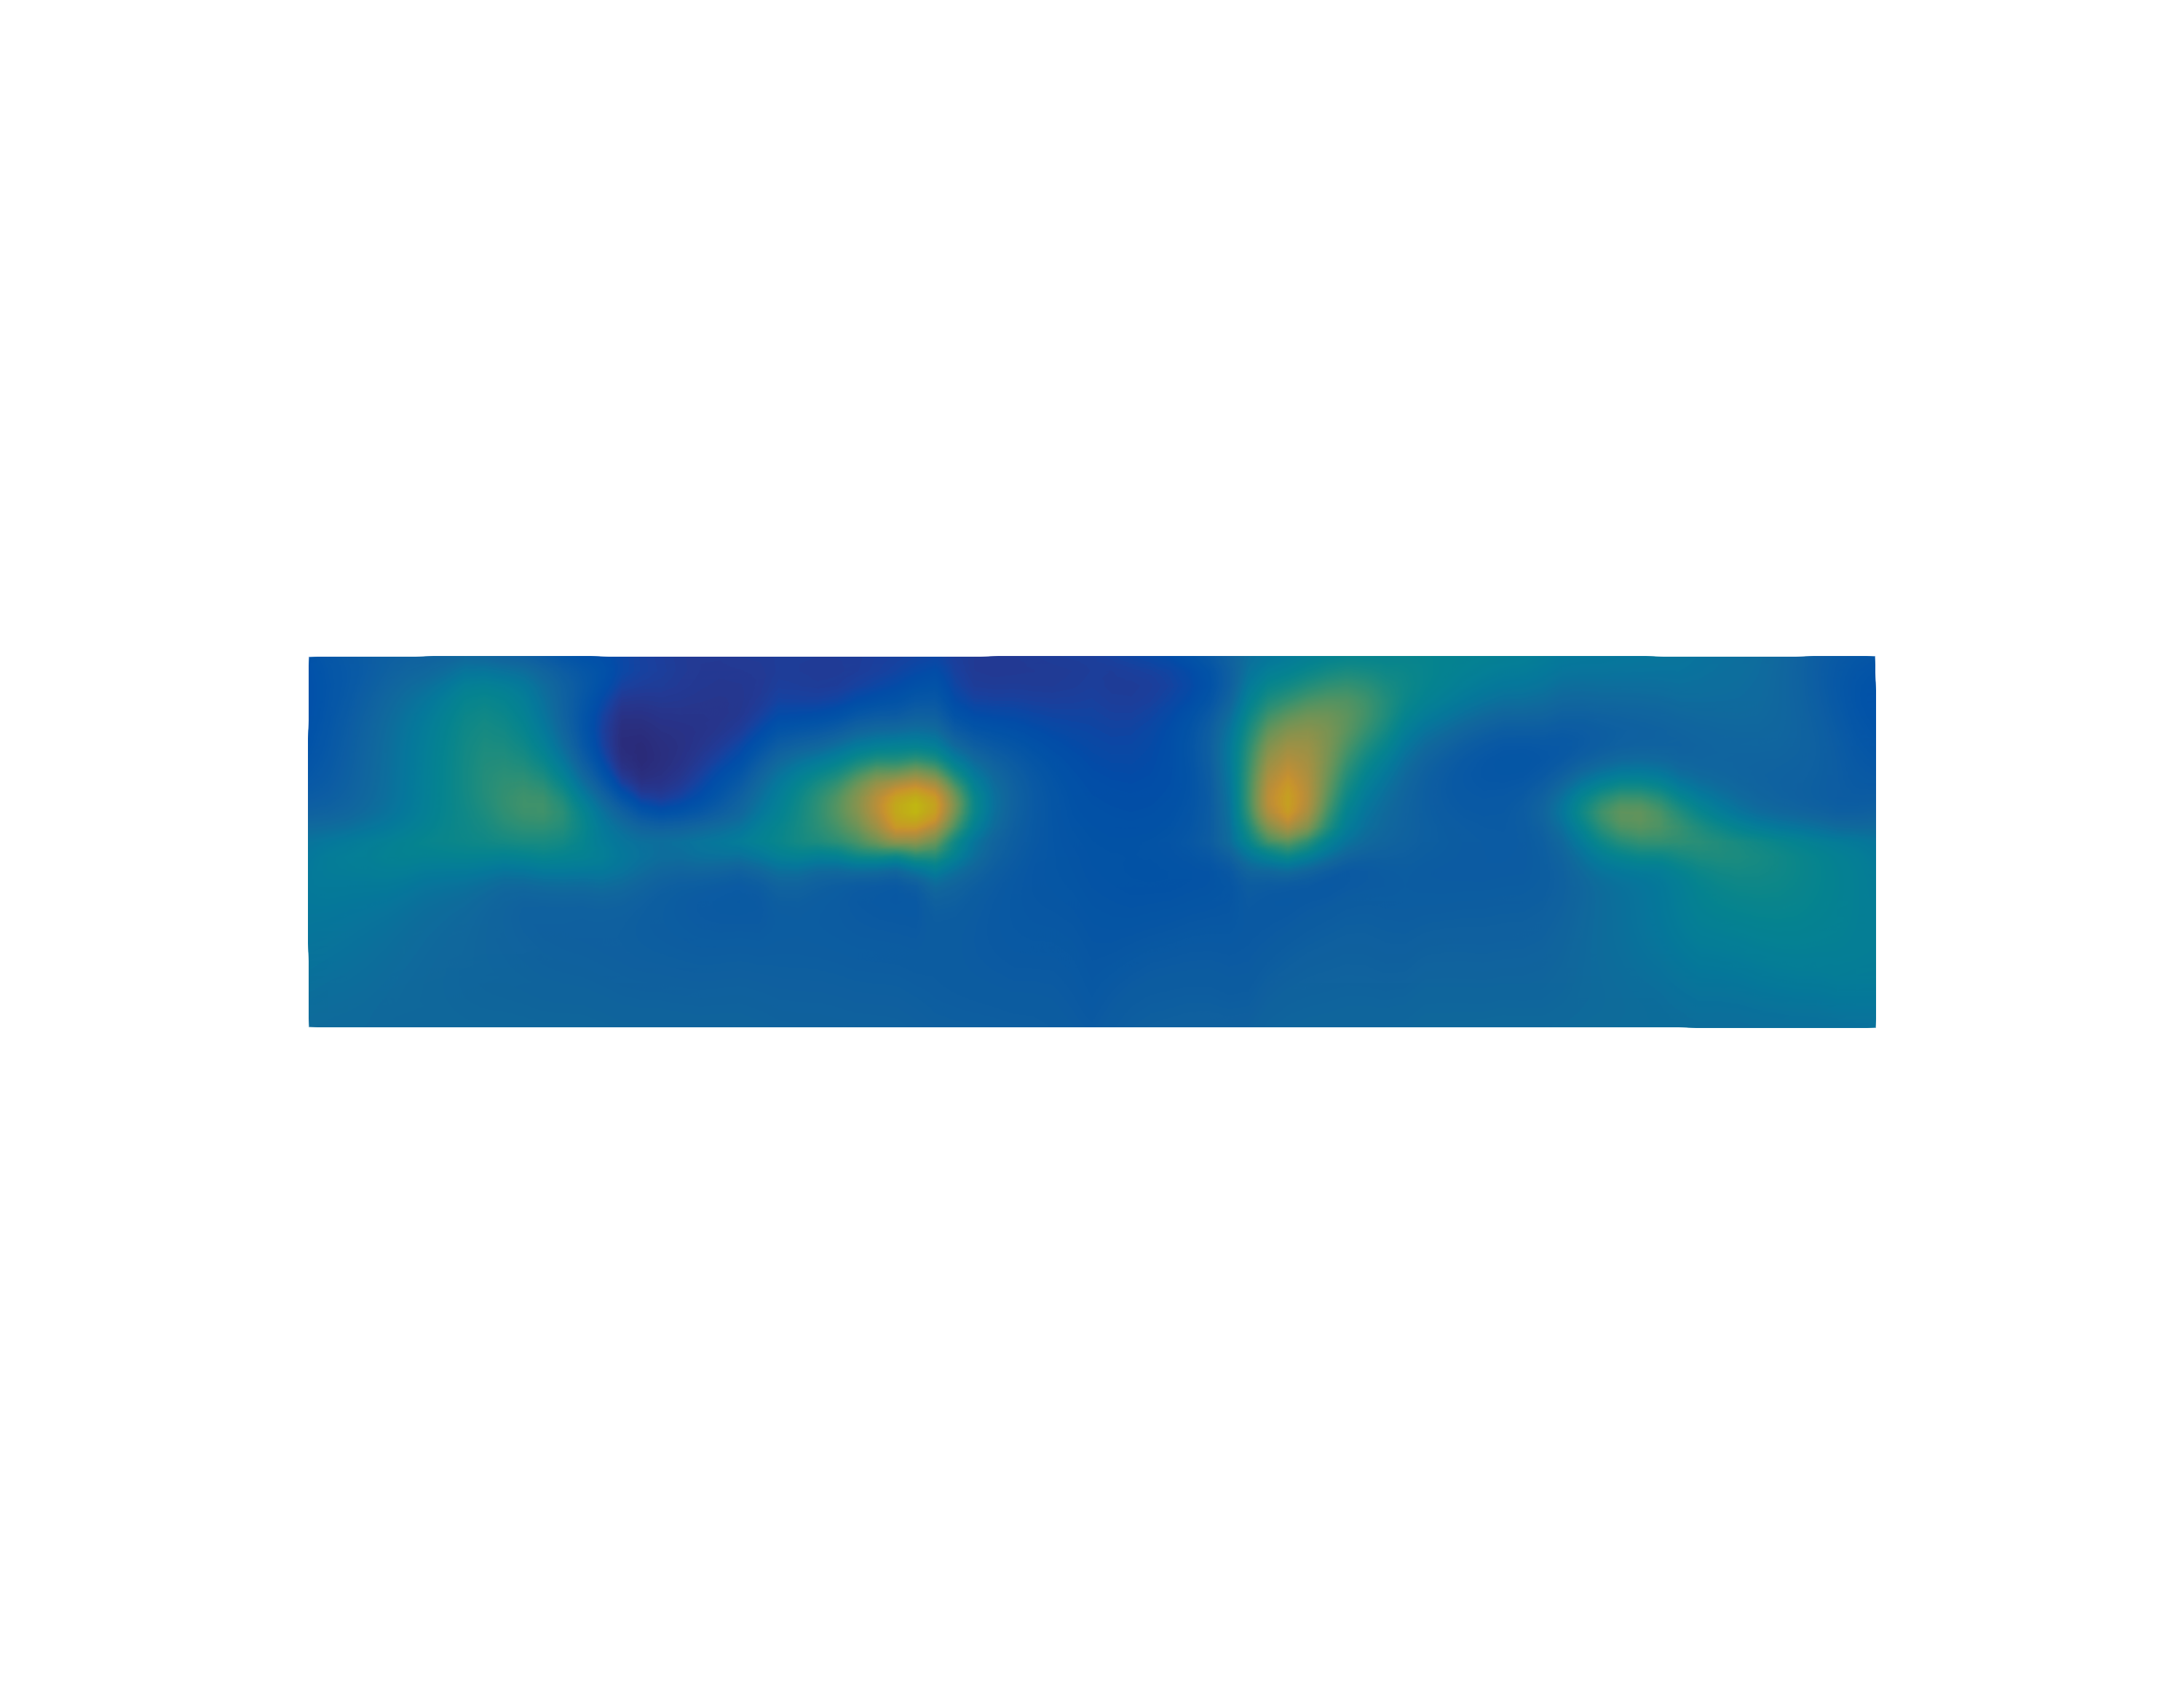
\includegraphics[width=0.9\textwidth]{../media/fourier/application/print/ab-0-2-concentration-acd.png}
        \caption{Anode $(1,2)$ désactivée}
      \end{center}
    \end{subfigure}

    \begin{multicols}{2}
        \begin{tikzpicture}
          \begin{axis}[
              colorbar,
              hide axis,
              scale only axis,
              height=0.10\textwidth,
              width=0.5\textwidth,
              colorbar horizontal,
              point meta min=0.0,
              point meta max=6.0,
              colorbar style={
                title=Vitesse $u_h$ [\si{\centi\meter\per\second}],
                width=4cm,
                height=0.3cm,
                xtick={0.0, 3.0, 6.0},
                at={(0.3\textwidth,0.4cm)},
                anchor=north
              }
            ]
            \addplot [] coordinates {(0,0)};
            \node (myfirstpic) at (0,0) {};
          \end{axis}
      \end{tikzpicture}\\
        \begin{tikzpicture}
          \begin{axis}[
              colorbar,
              hide axis,
              scale only axis,
              height=0.10\textwidth,
              width=0.5\textwidth,
              colorbar horizontal,
              point meta min=2.26,
              point meta max=5.43,
              colorbar style={
                title=Concentration $c$ [w\%],
                width=4cm,
                height=0.3cm,
                xtick={2.26, 4, 5.43},
                at={(0.3\textwidth,0.4cm)},
                anchor=north
              }
            ]
            \addplot [] coordinates {(0,0)};
            \node (myfirstpic) at (0,0) {};
          \end{axis}
        \end{tikzpicture}
    \end{multicols}

    \caption{Champs de vitesse stationnaire $u^{\mathrm{S3D}}$ (haut) et de
      concentration $c^\mathrm{S3D}$ (bas) dans l'ACD de la cuve
      AP32 pour différentes configurations du plan anodique.}
    \label{fig:f3d-deactivated-a}
  \end{center}
\end{figure}

\begin{figure}[!h]
  \begin{center}
    \begin{subfigure}[t]{\textwidth}
      \begin{center}
        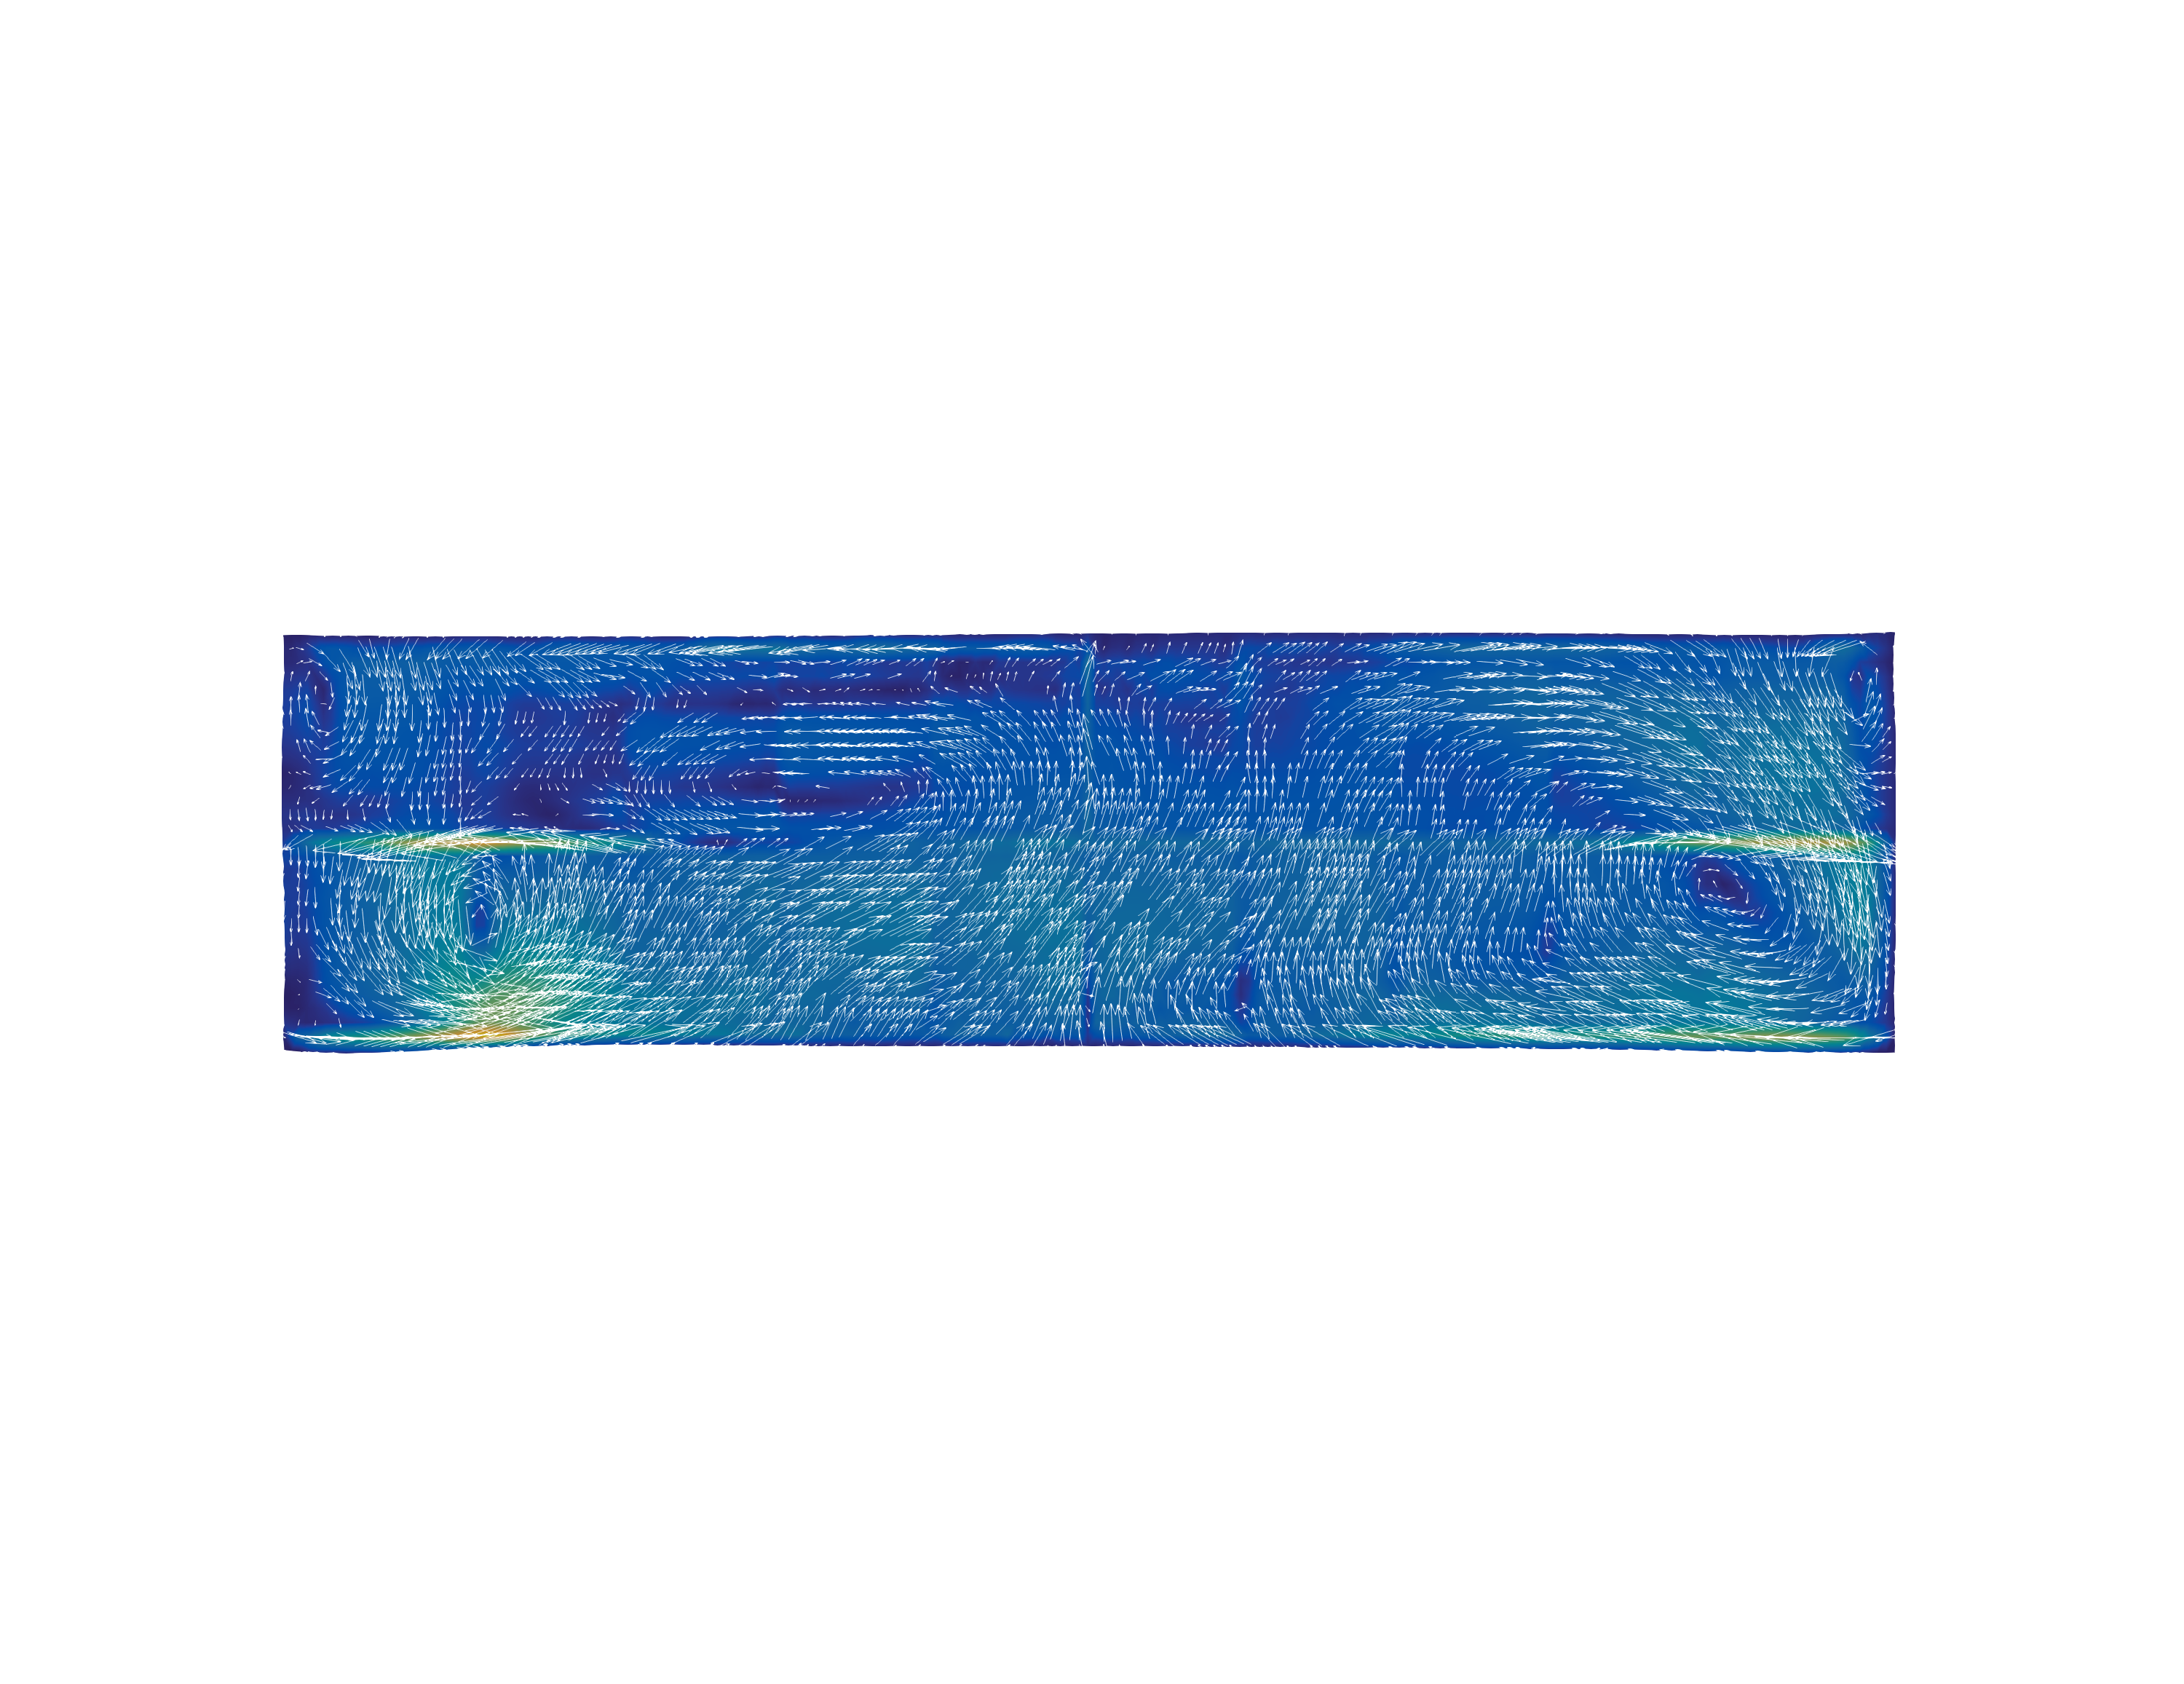
\includegraphics[width=0.9\textwidth]{../media/fourier/application/print/ab-1-1-velocity-acd.png}
        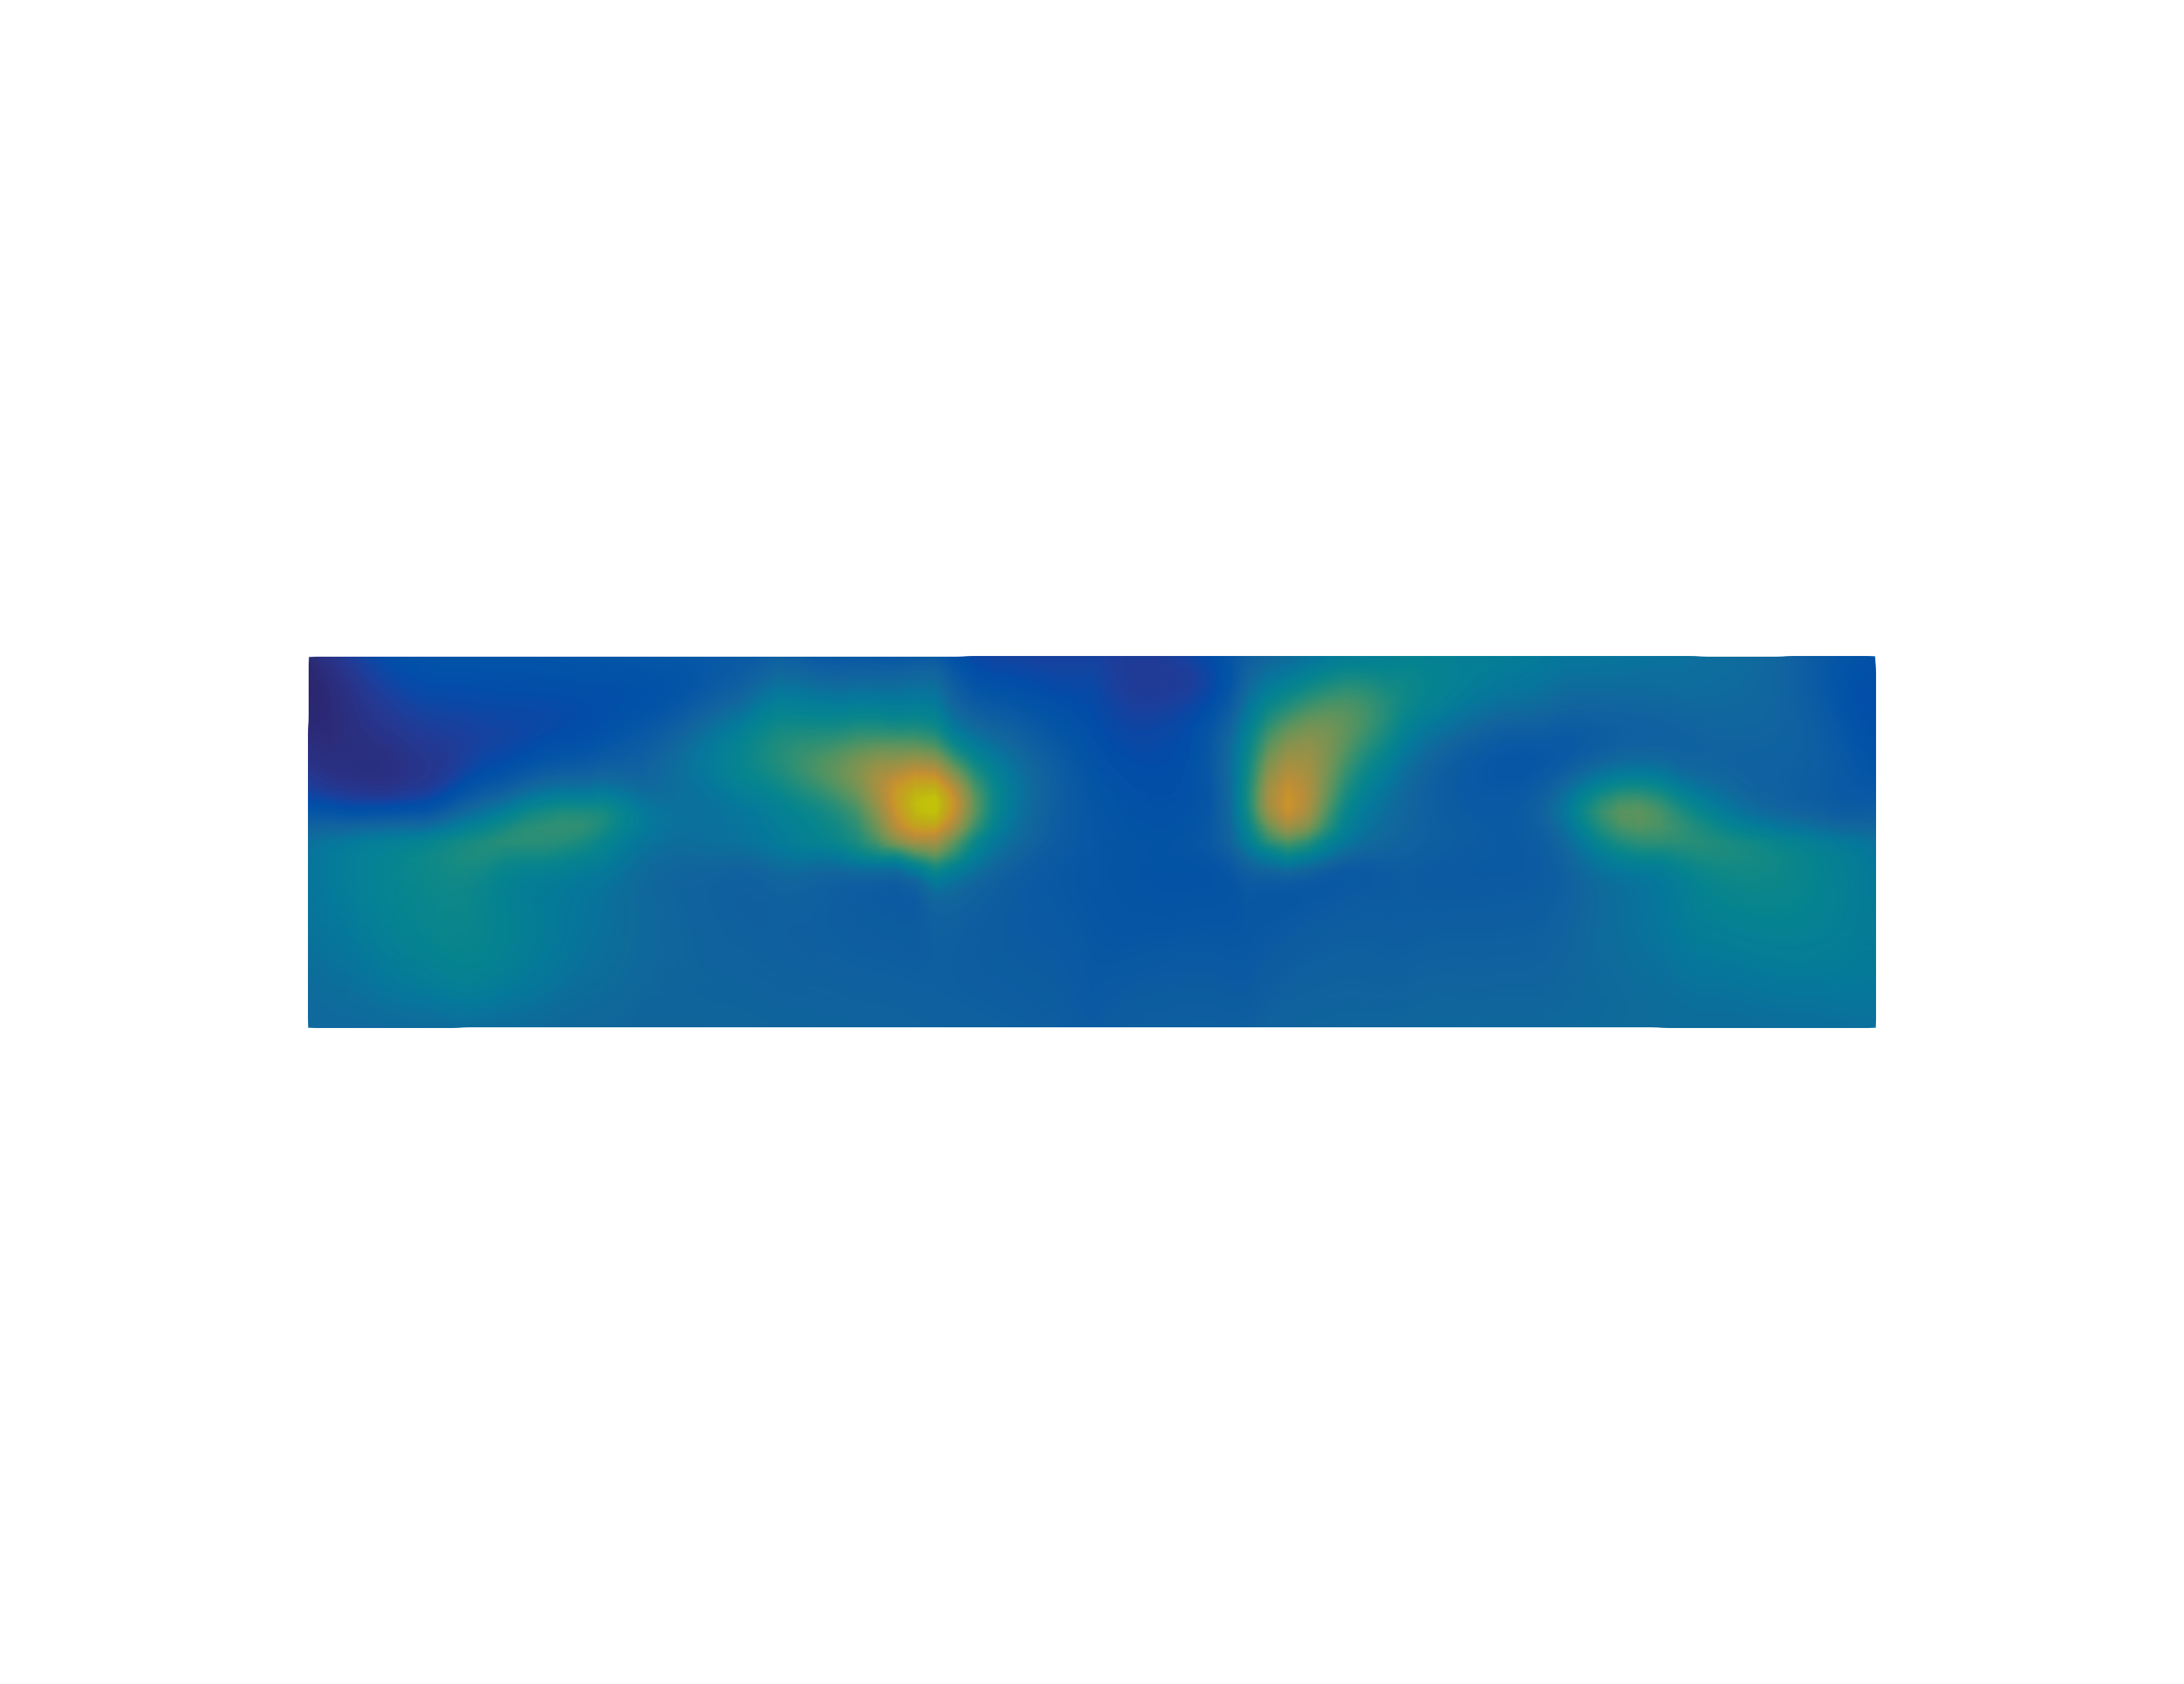
\includegraphics[width=0.9\textwidth]{../media/fourier/application/print/ab-1-1-concentration-acd.png}
        \caption{Anode $(2,1)$ désactivée}
      \end{center}
    \end{subfigure}
    \begin{subfigure}[t]{\textwidth}
      \begin{center}
        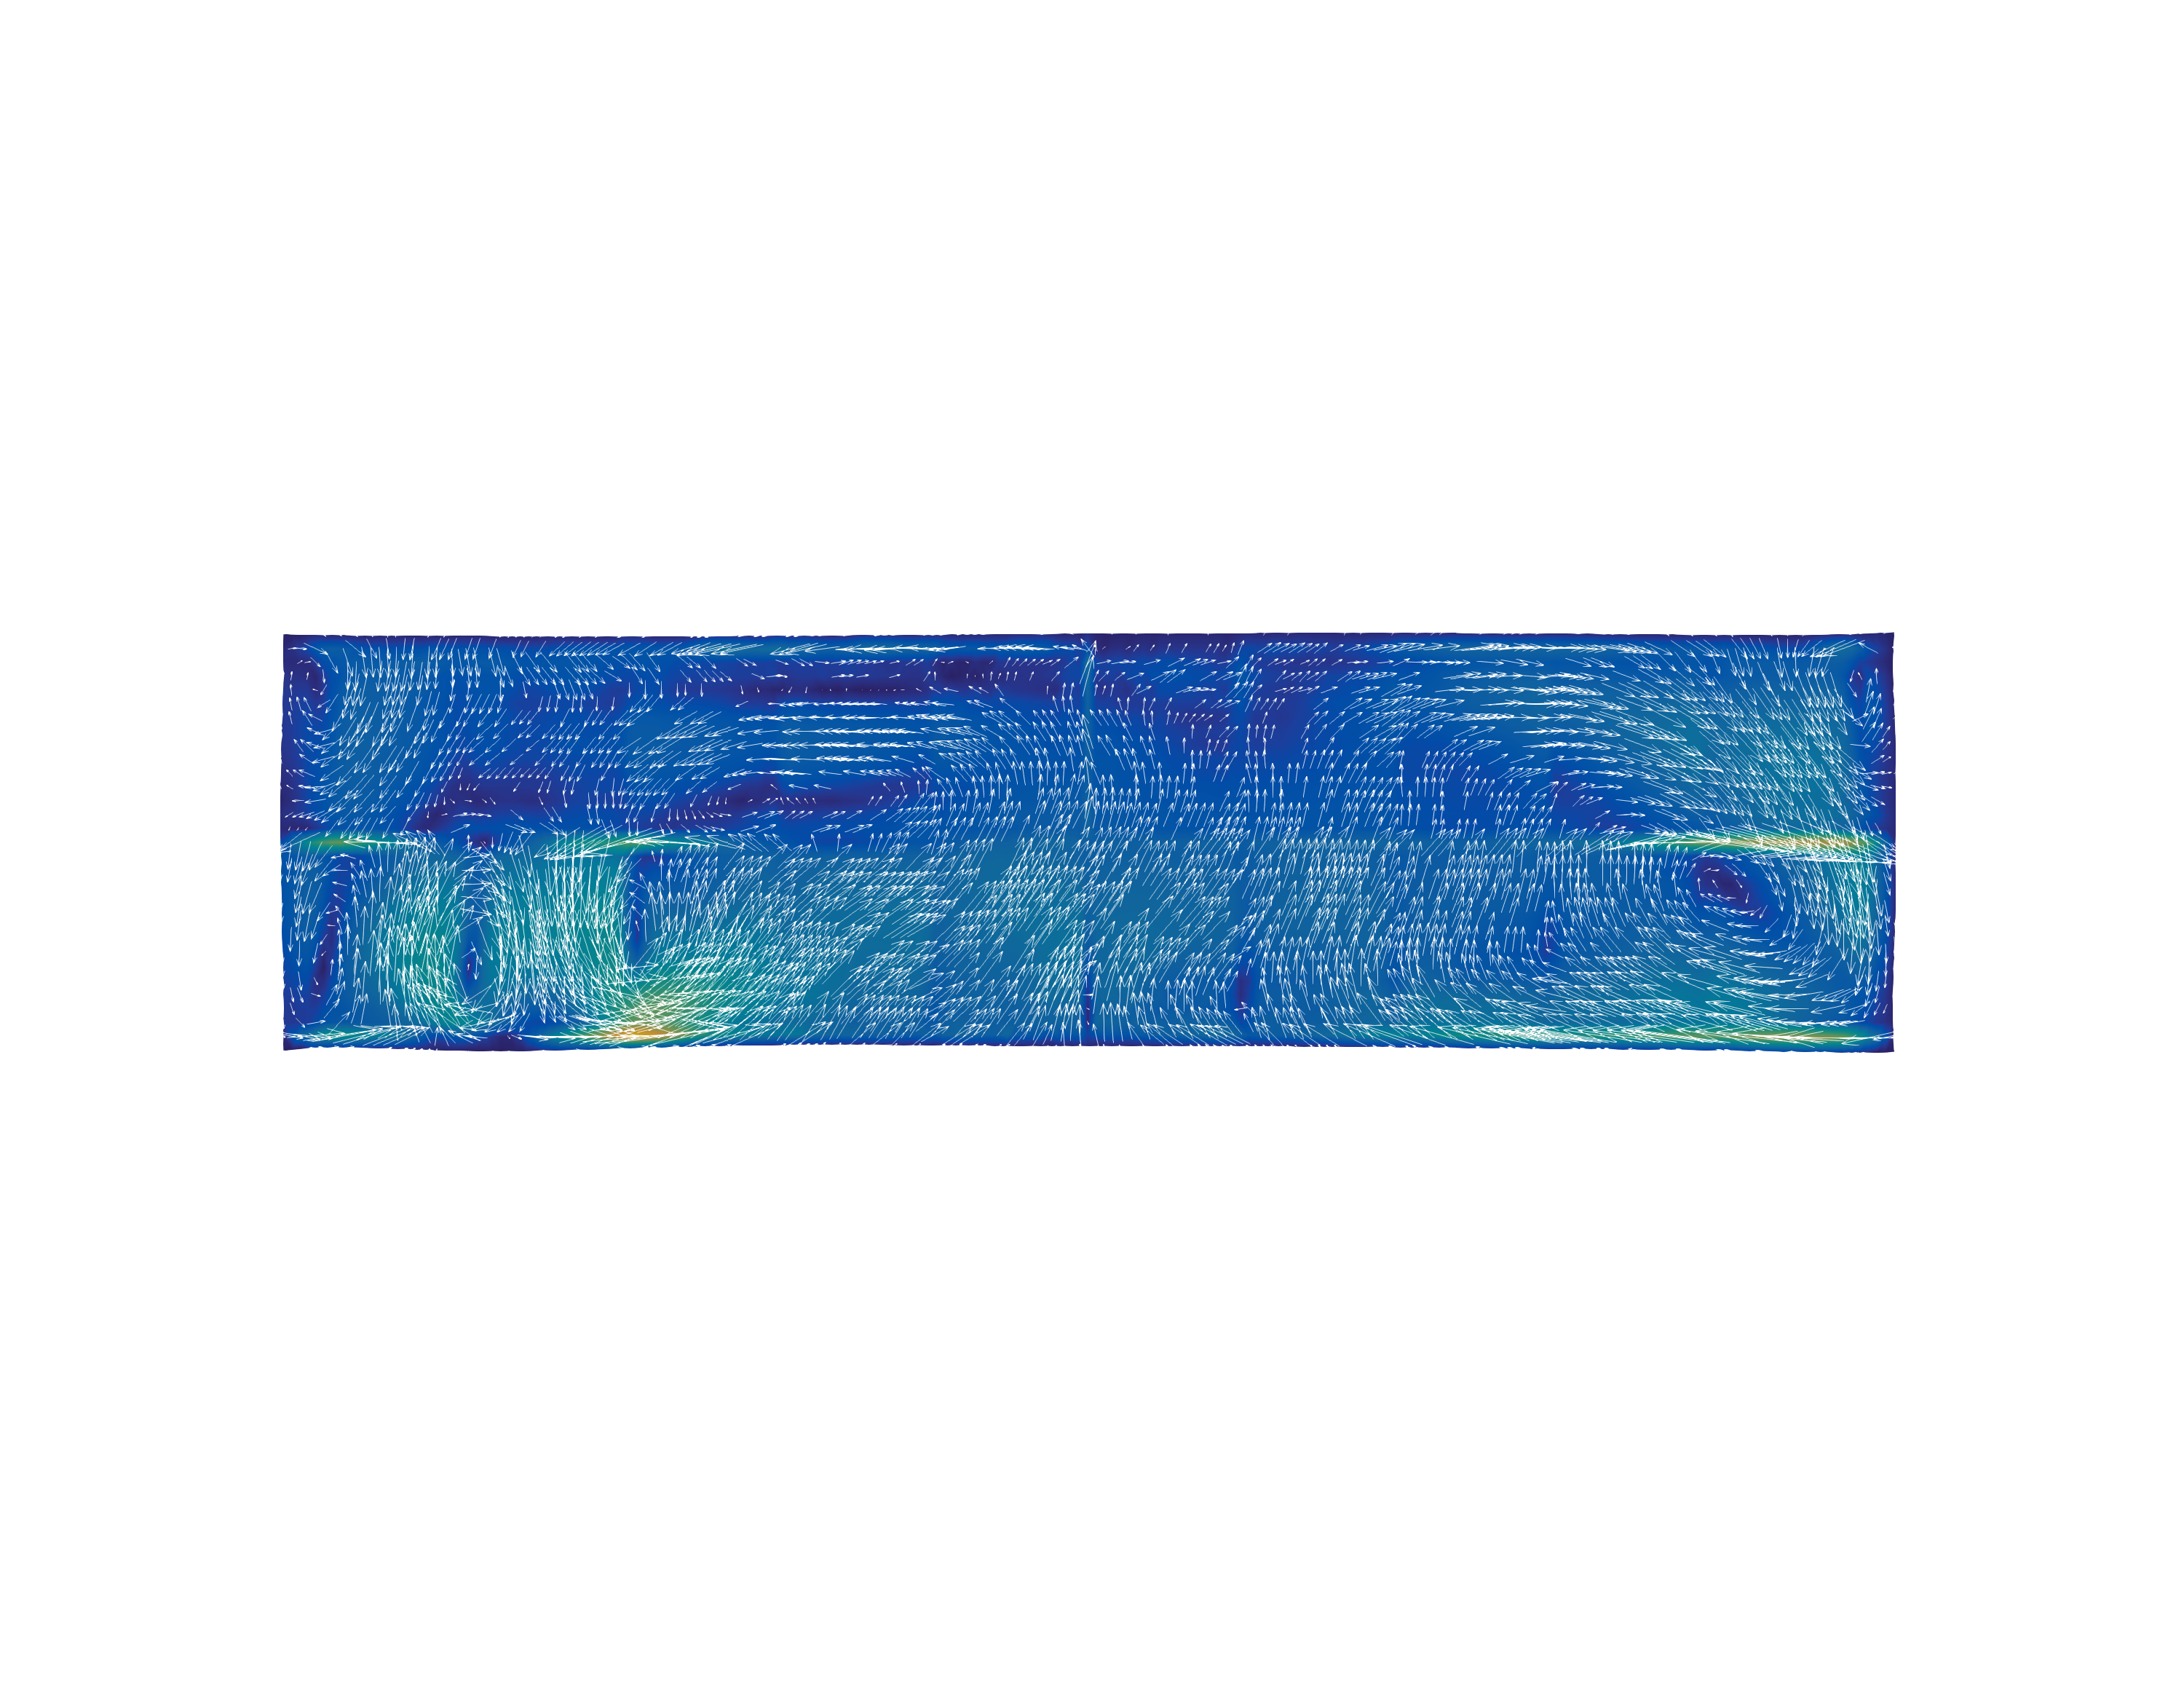
\includegraphics[width=0.9\textwidth]{../media/fourier/application/print/ab-1-2-velocity-acd.png}
        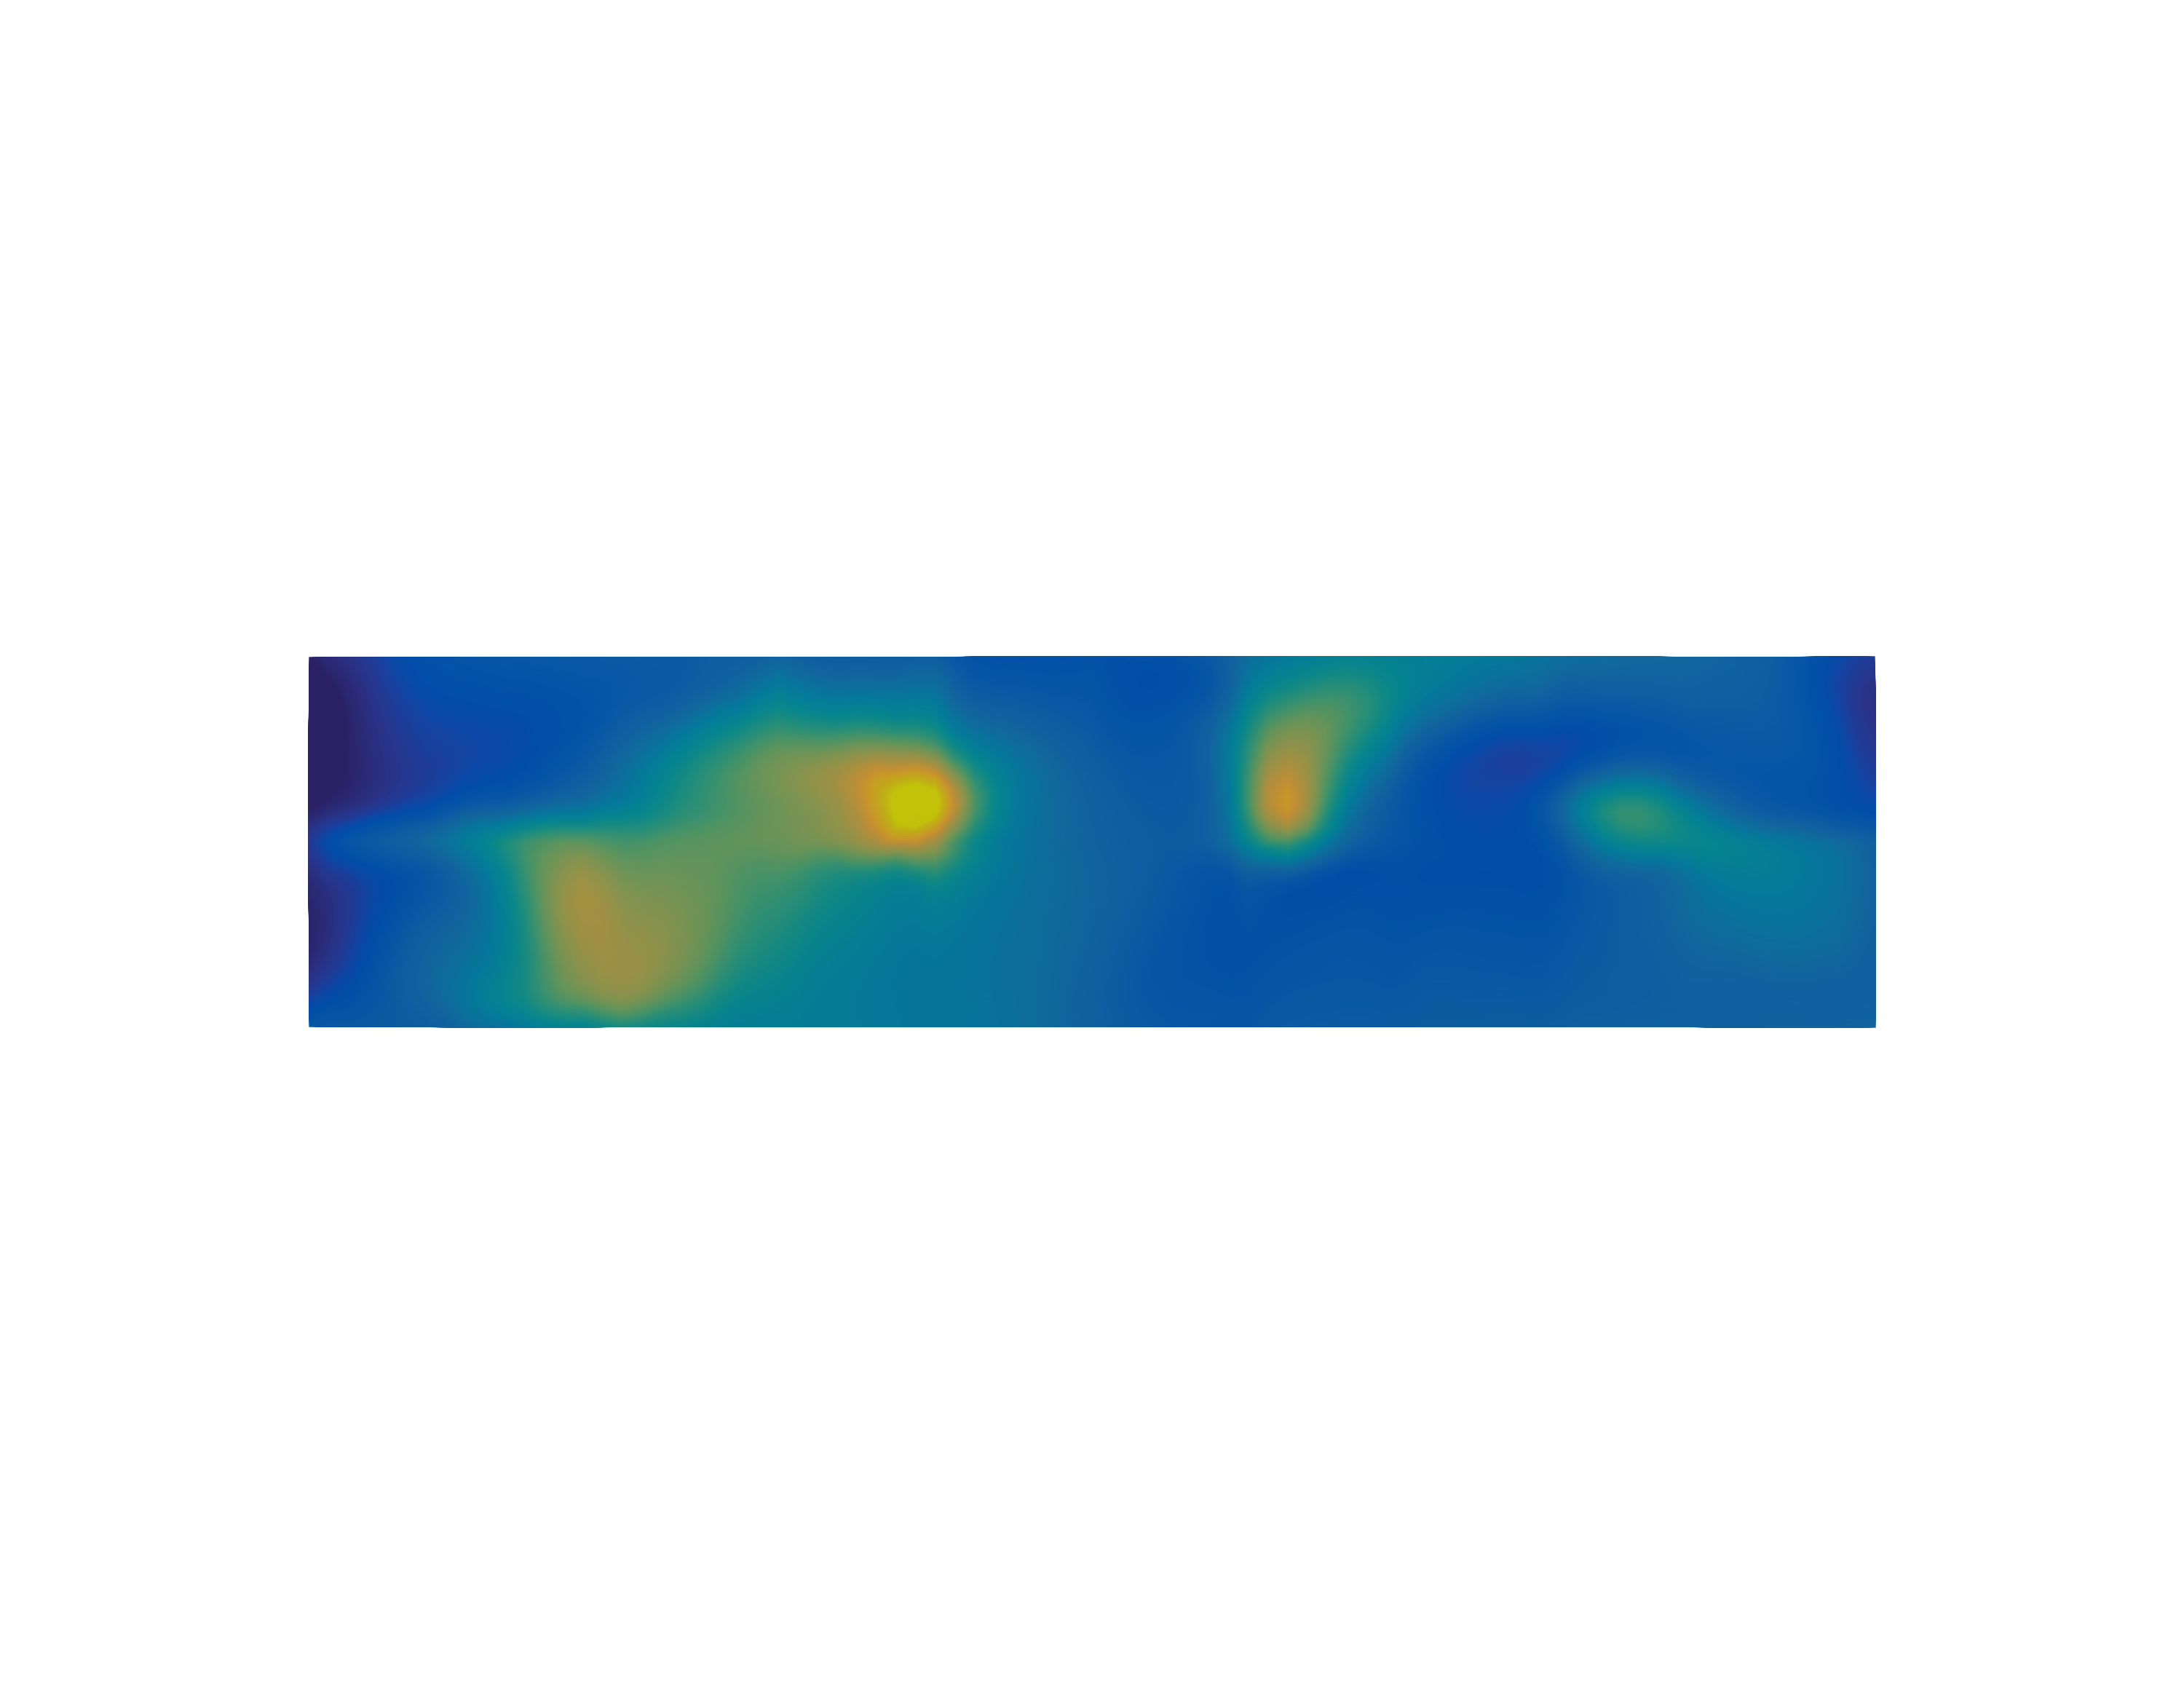
\includegraphics[width=0.9\textwidth]{../media/fourier/application/print/ab-1-2-concentration-acd.png}
        \caption{Anode $(2,2)$ désactivée}
      \end{center}
    \end{subfigure}

    \begin{multicols}{2}
        \begin{tikzpicture}
          \begin{axis}[
              colorbar,
              hide axis,
              scale only axis,
              height=0.10\textwidth,
              width=0.5\textwidth,
              colorbar horizontal,
              point meta min=0.0,
              point meta max=6.0,
              colorbar style={
                title=Vitesse $u_h$ [\si{\centi\meter\per\second}],
                width=4cm,
                height=0.3cm,
                xtick={0.0, 3.0, 6.0},
                at={(0.3\textwidth,0.4cm)},
                anchor=north
              }
            ]
            \addplot [] coordinates {(0,0)};
            \node (myfirstpic) at (0,0) {};
          \end{axis}
      \end{tikzpicture}\\
        \begin{tikzpicture}
          \begin{axis}[
              colorbar,
              hide axis,
              scale only axis,
              height=0.10\textwidth,
              width=0.5\textwidth,
              colorbar horizontal,
              point meta min=2.26,
              point meta max=5.43,
              colorbar style={
                title=Concentration $c$ [w\%],
                width=4cm,
                height=0.3cm,
                xtick={2.26, 4, 5.43},
                at={(0.3\textwidth,0.4cm)},
                anchor=north
              }
            ]
            \addplot [] coordinates {(0,0)};
            \node (myfirstpic) at (0,0) {};
          \end{axis}
        \end{tikzpicture}
    \end{multicols}

    \caption{Champs de vitesse stationnaire $u^{\mathrm{S3D}}$ (haut) et de
      concentration $c^\mathrm{S3D}$ (bas) dans l'ACD de la cuve
      AP32 pour différentes configurations du plan anodique.}
    \label{fig:f3d-deactivated-b}
  \end{center}
\end{figure}
%


\begin{figure}[!h]
  \begin{center}
    \begin{subfigure}[t]{\textwidth}
      \begin{center}
        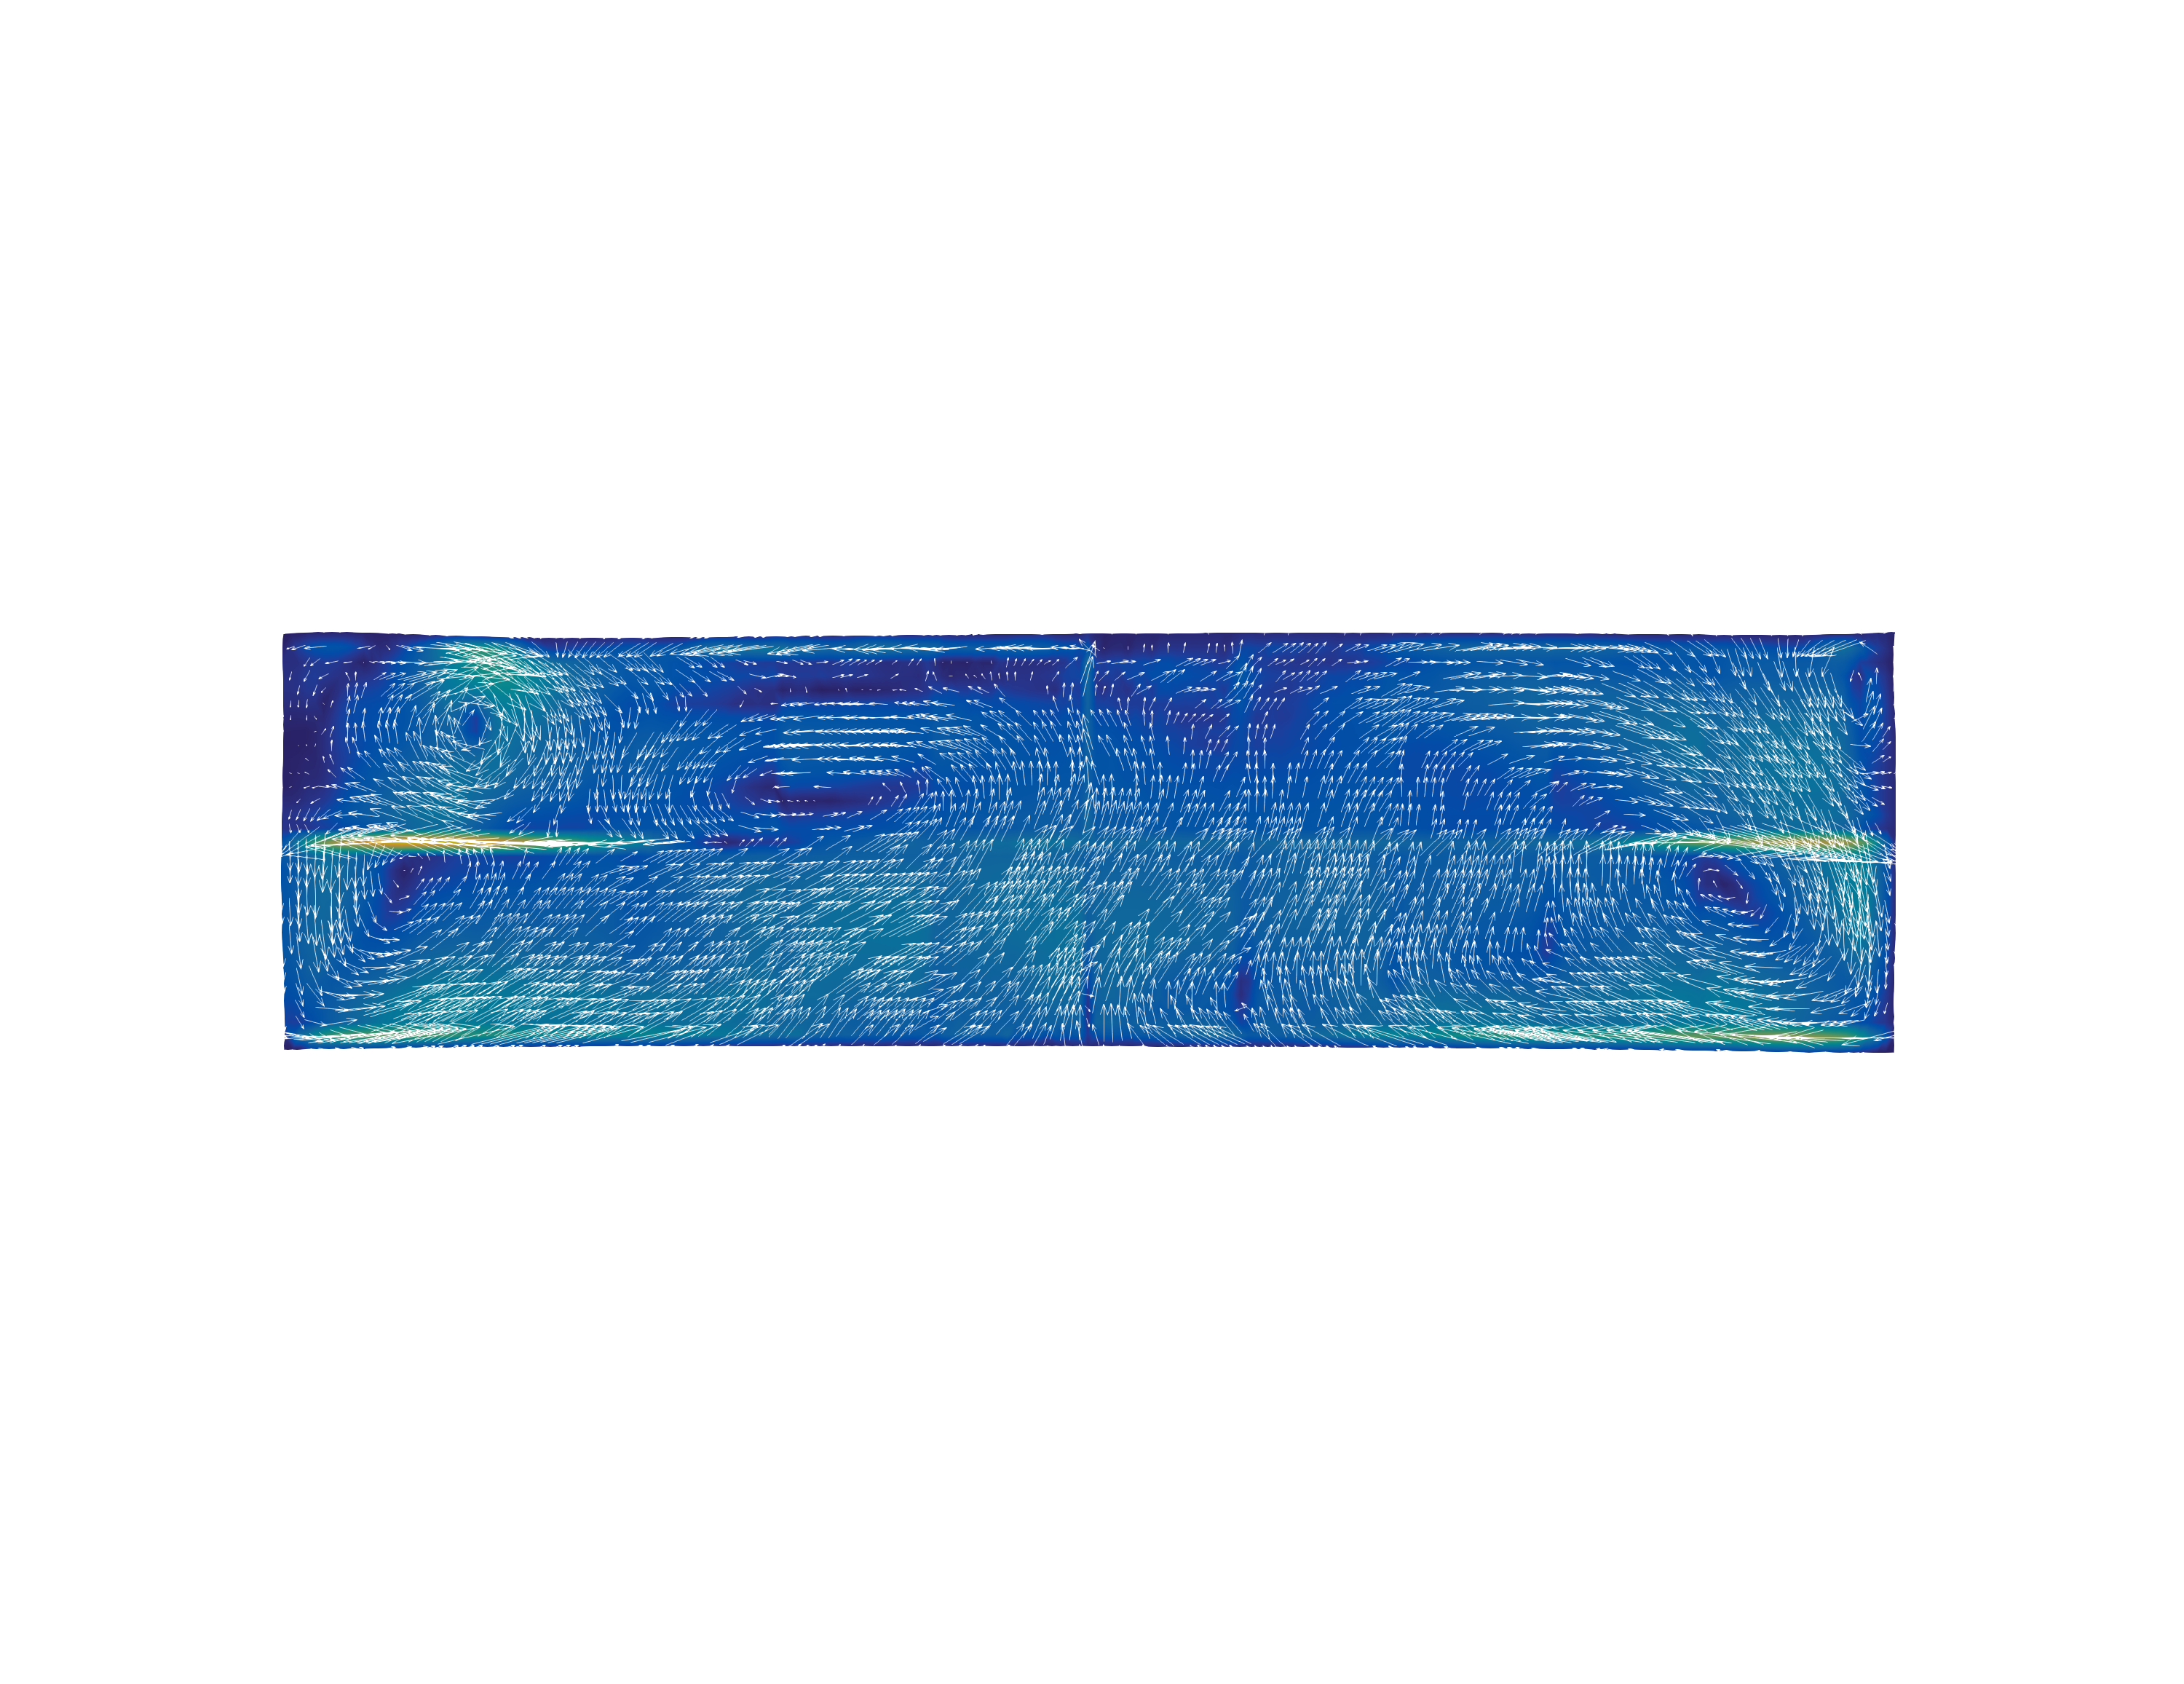
\includegraphics[width=0.9\textwidth]{../media/fourier/application/print/ab-0-1-velocity-acd.png}
        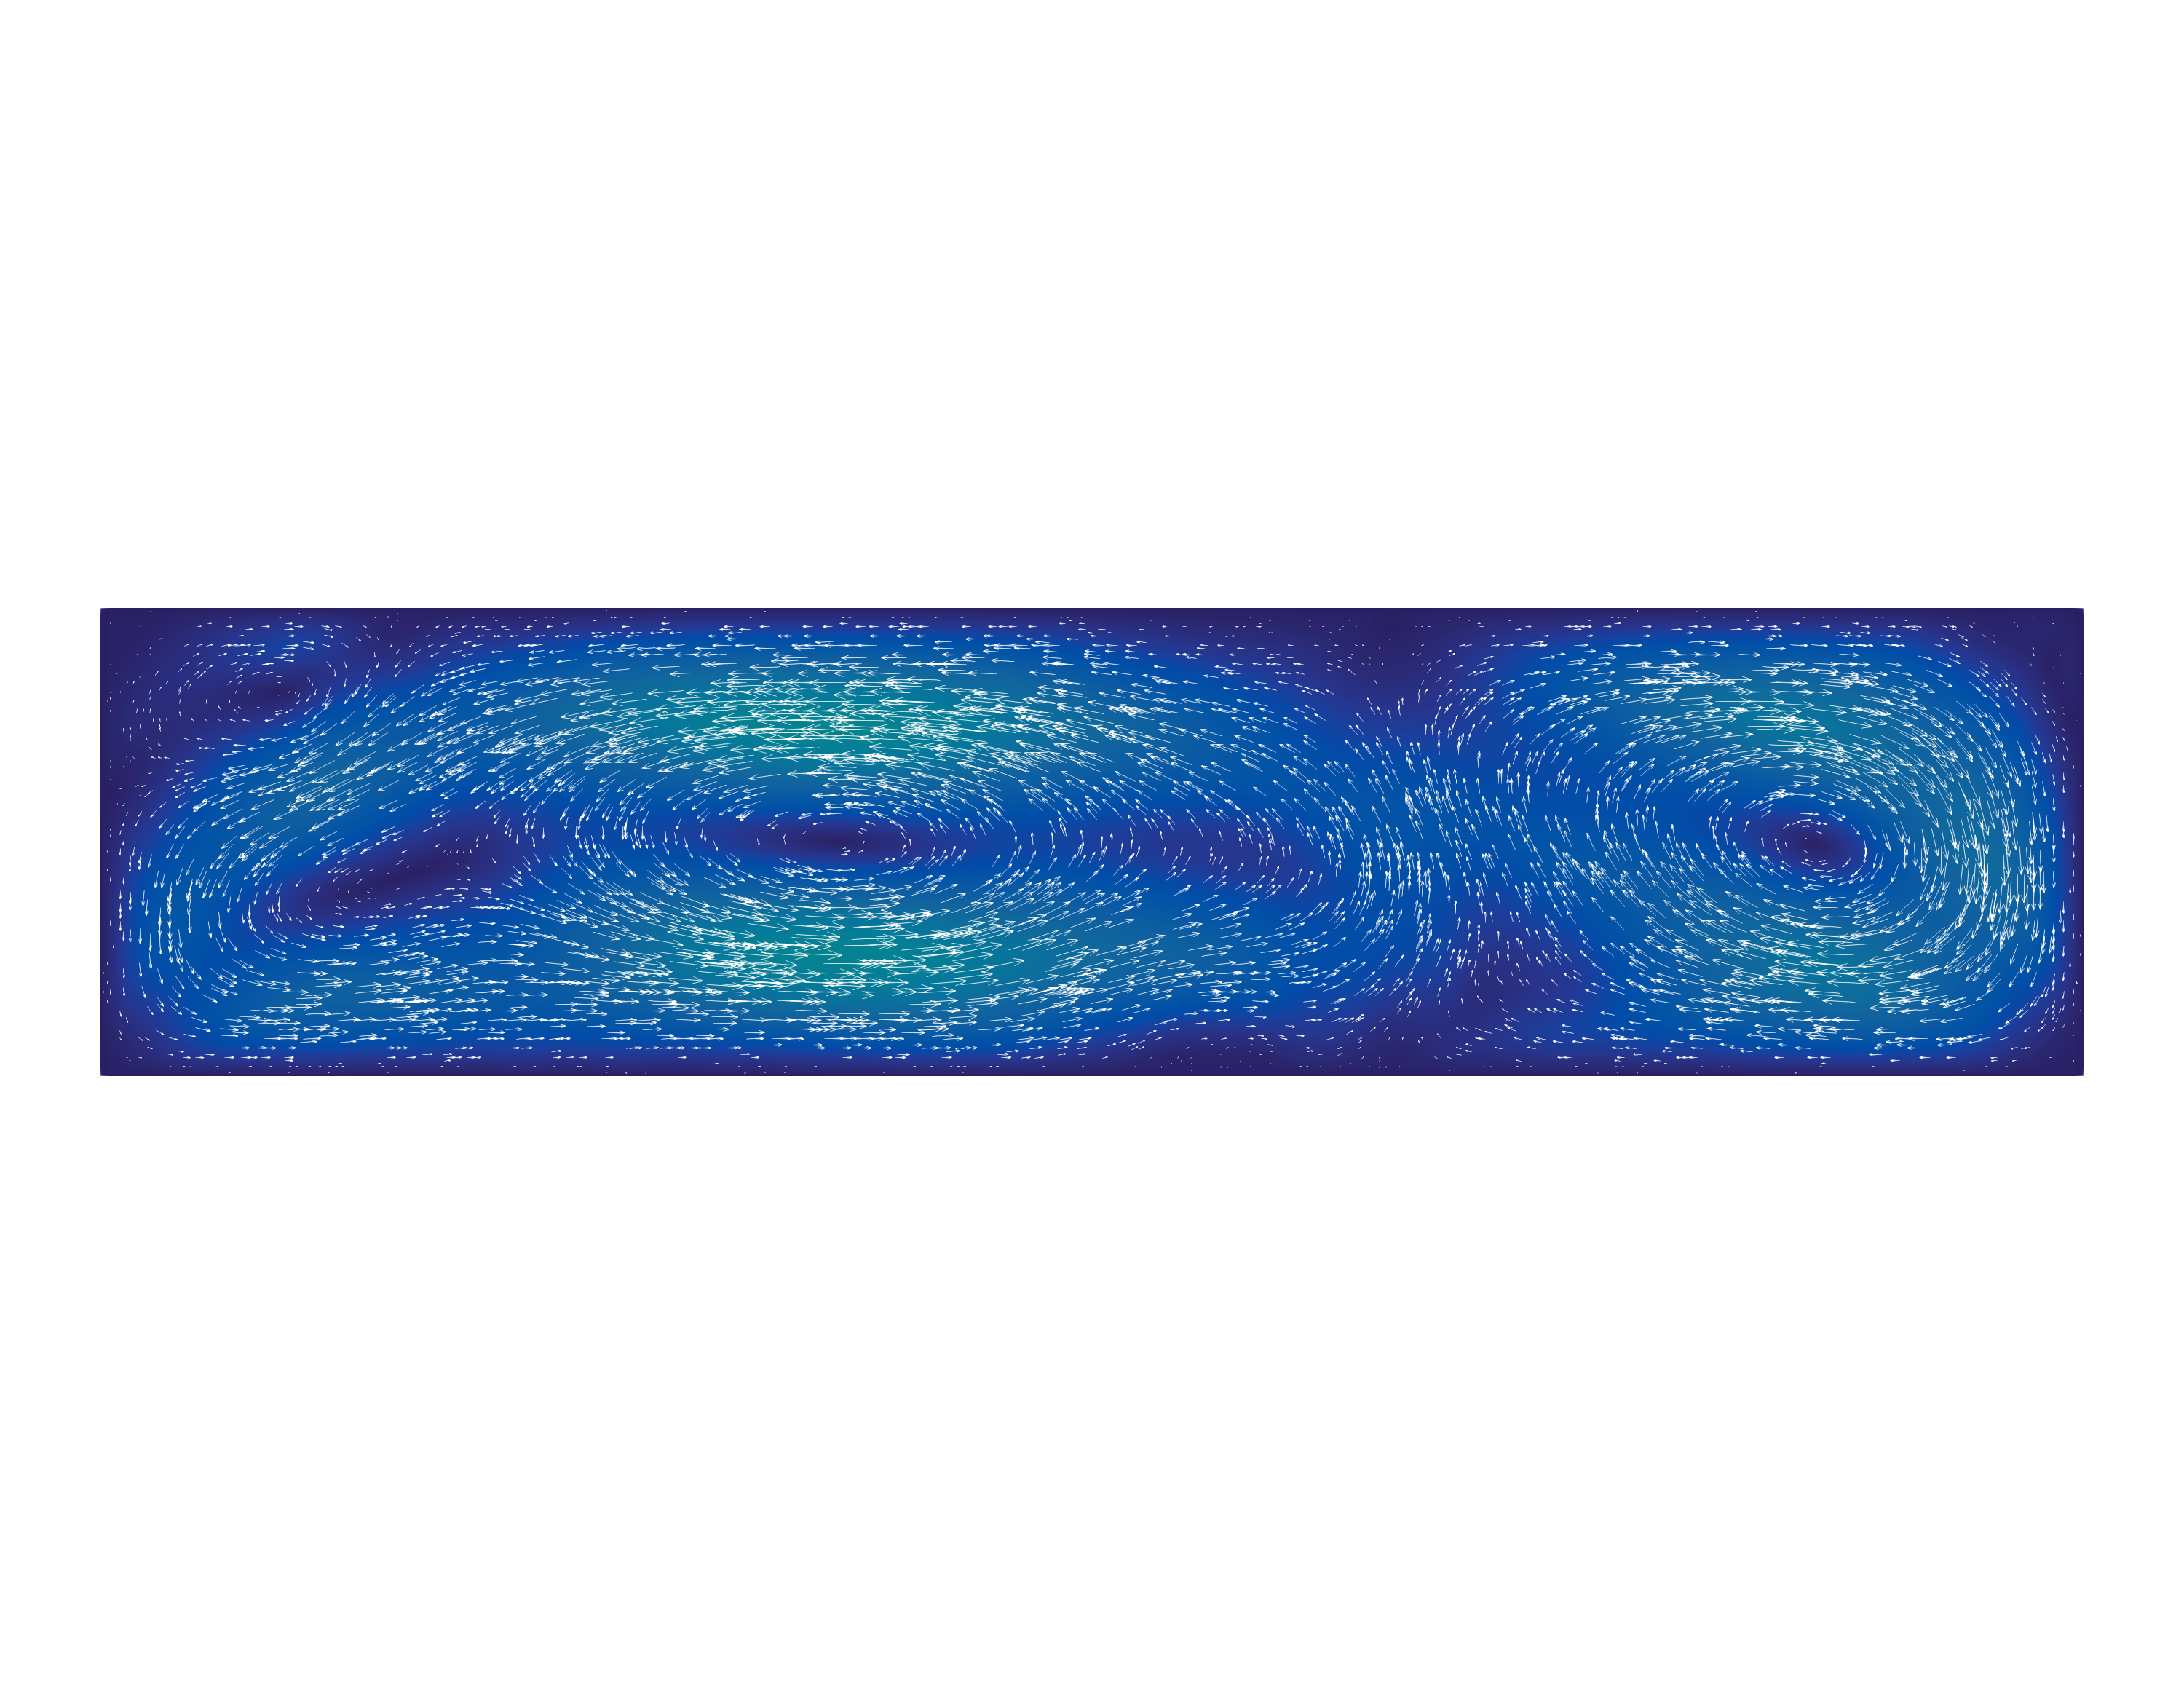
\includegraphics[width=0.9\textwidth]{../media/fourier/application/print/ab-0-1-velocity-harm.png}
        \caption{Anode $(1,1)$ désactivée}
        \label{fig:}
      \end{center}
    \end{subfigure}

    \begin{subfigure}[t]{\textwidth}
      \begin{center}
        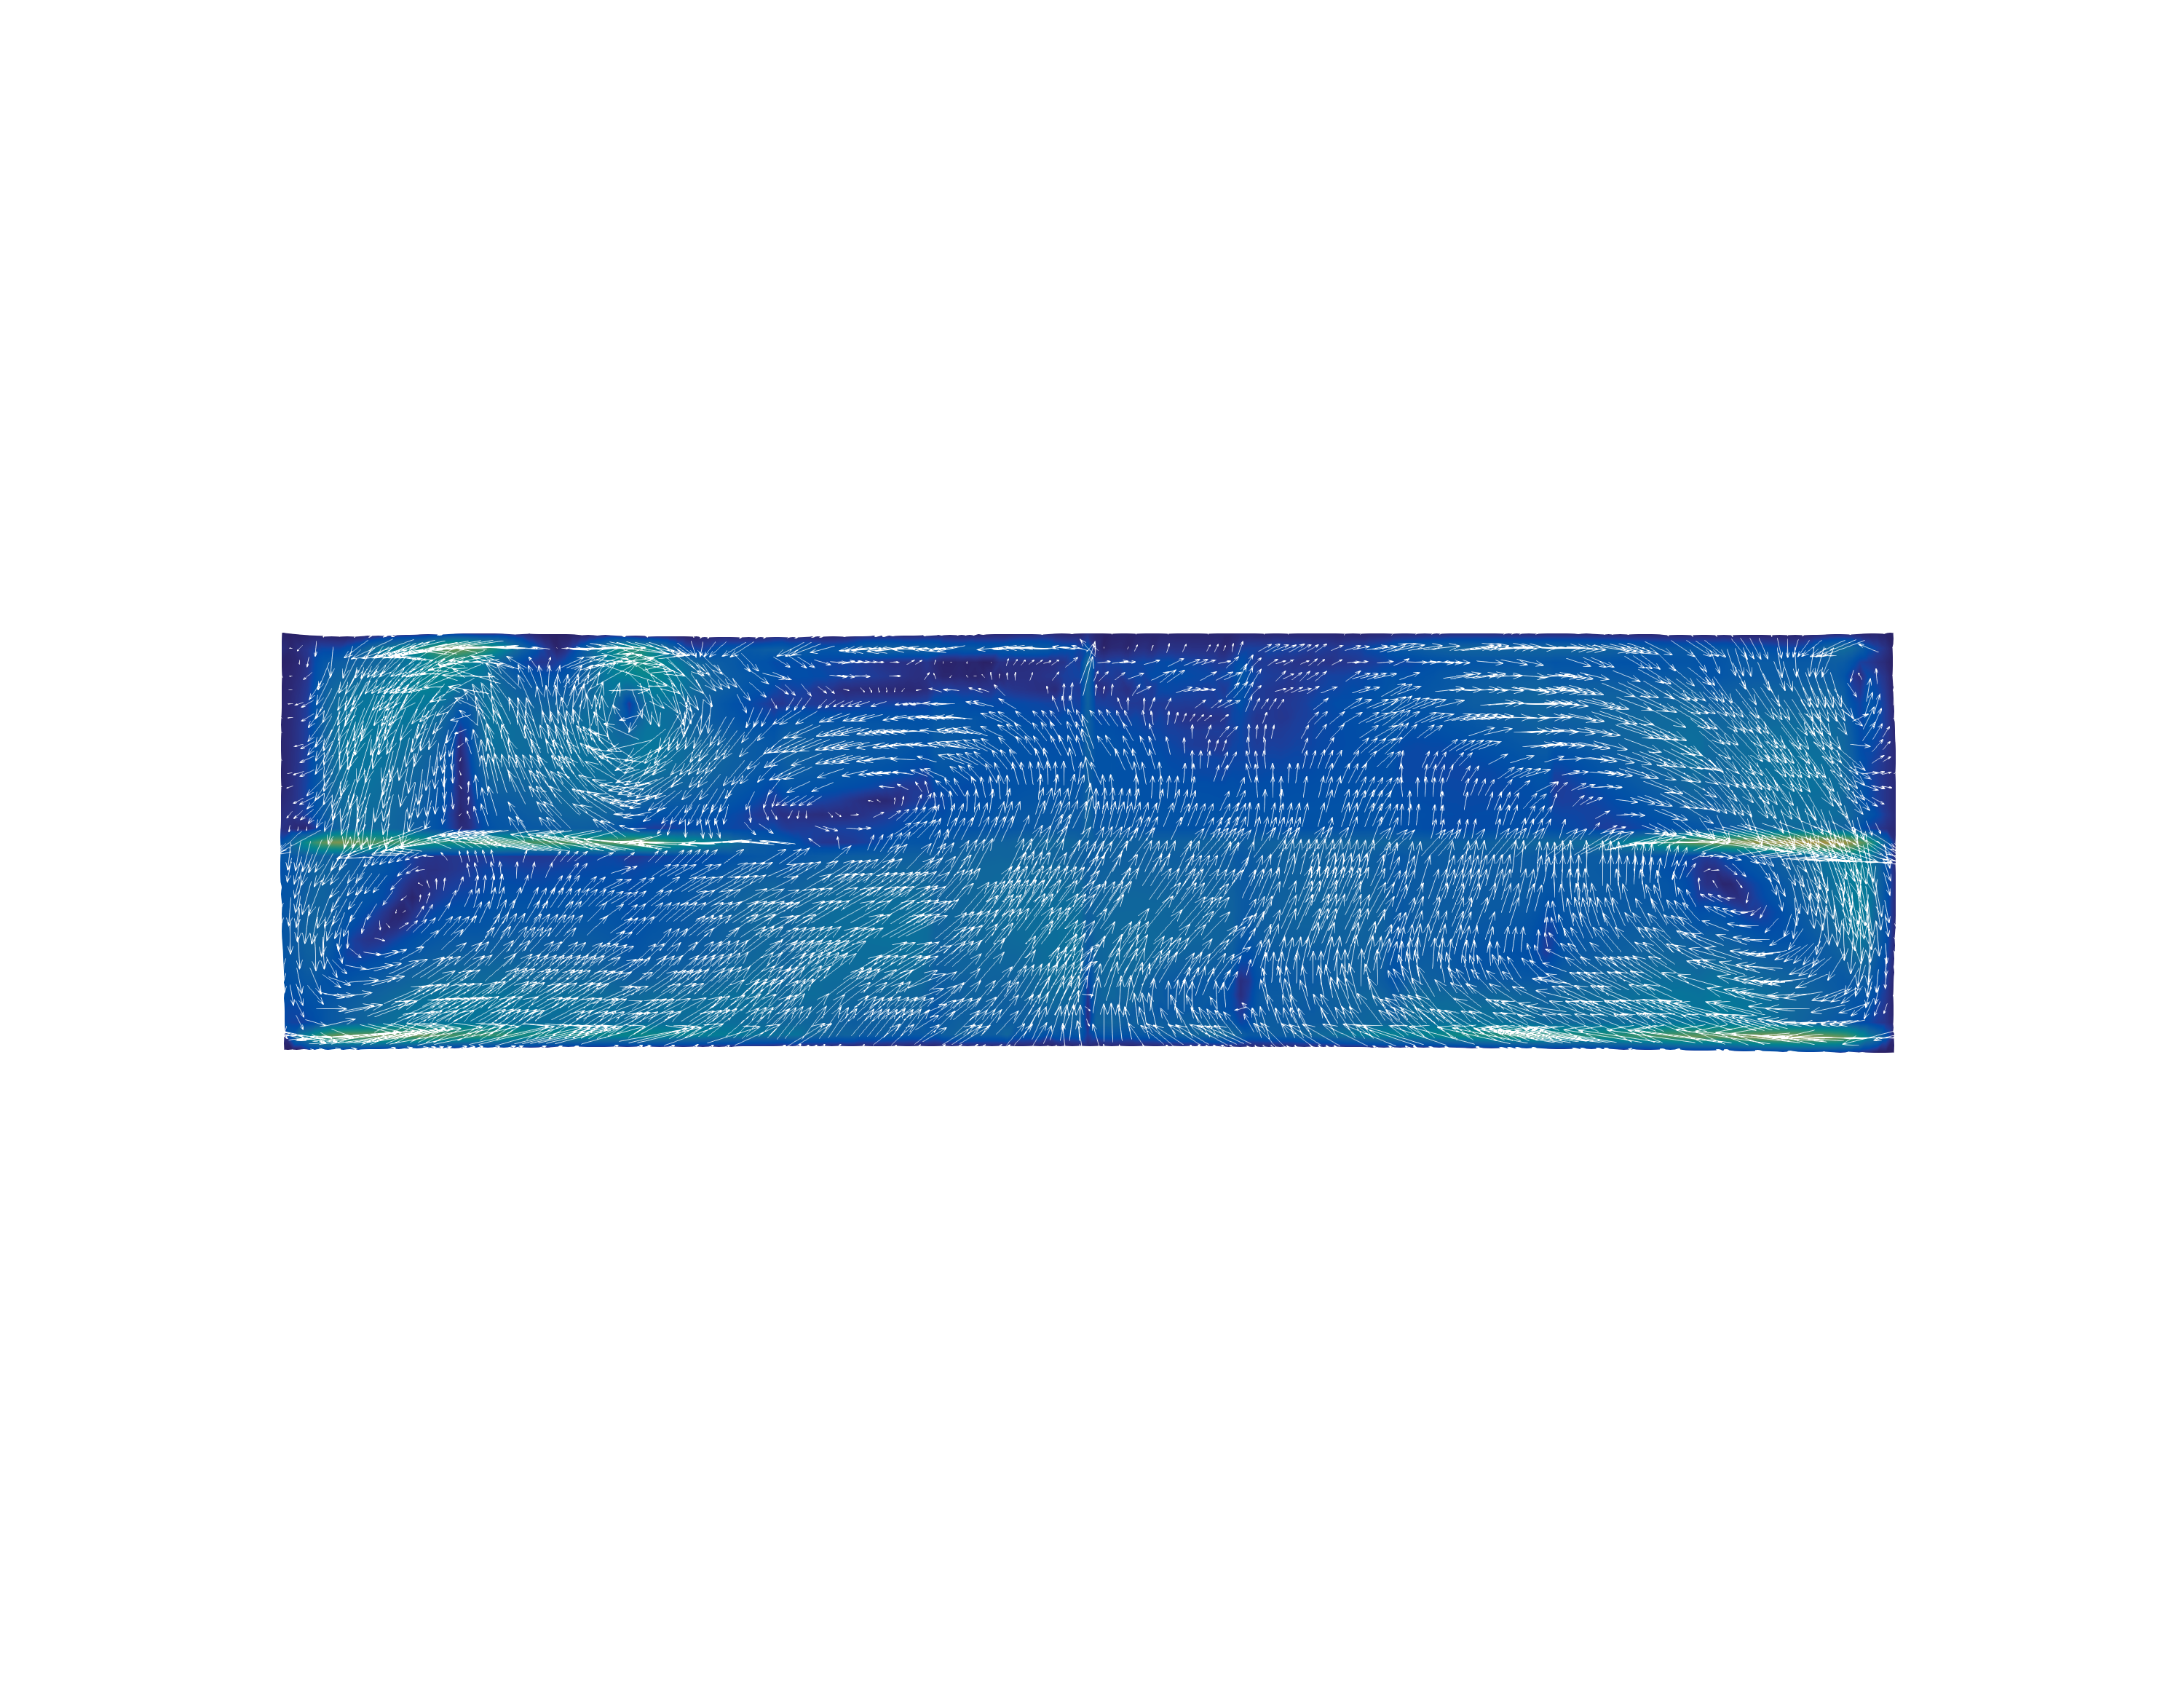
\includegraphics[width=0.9\textwidth]{../media/fourier/application/print/ab-0-2-velocity-acd.png}
        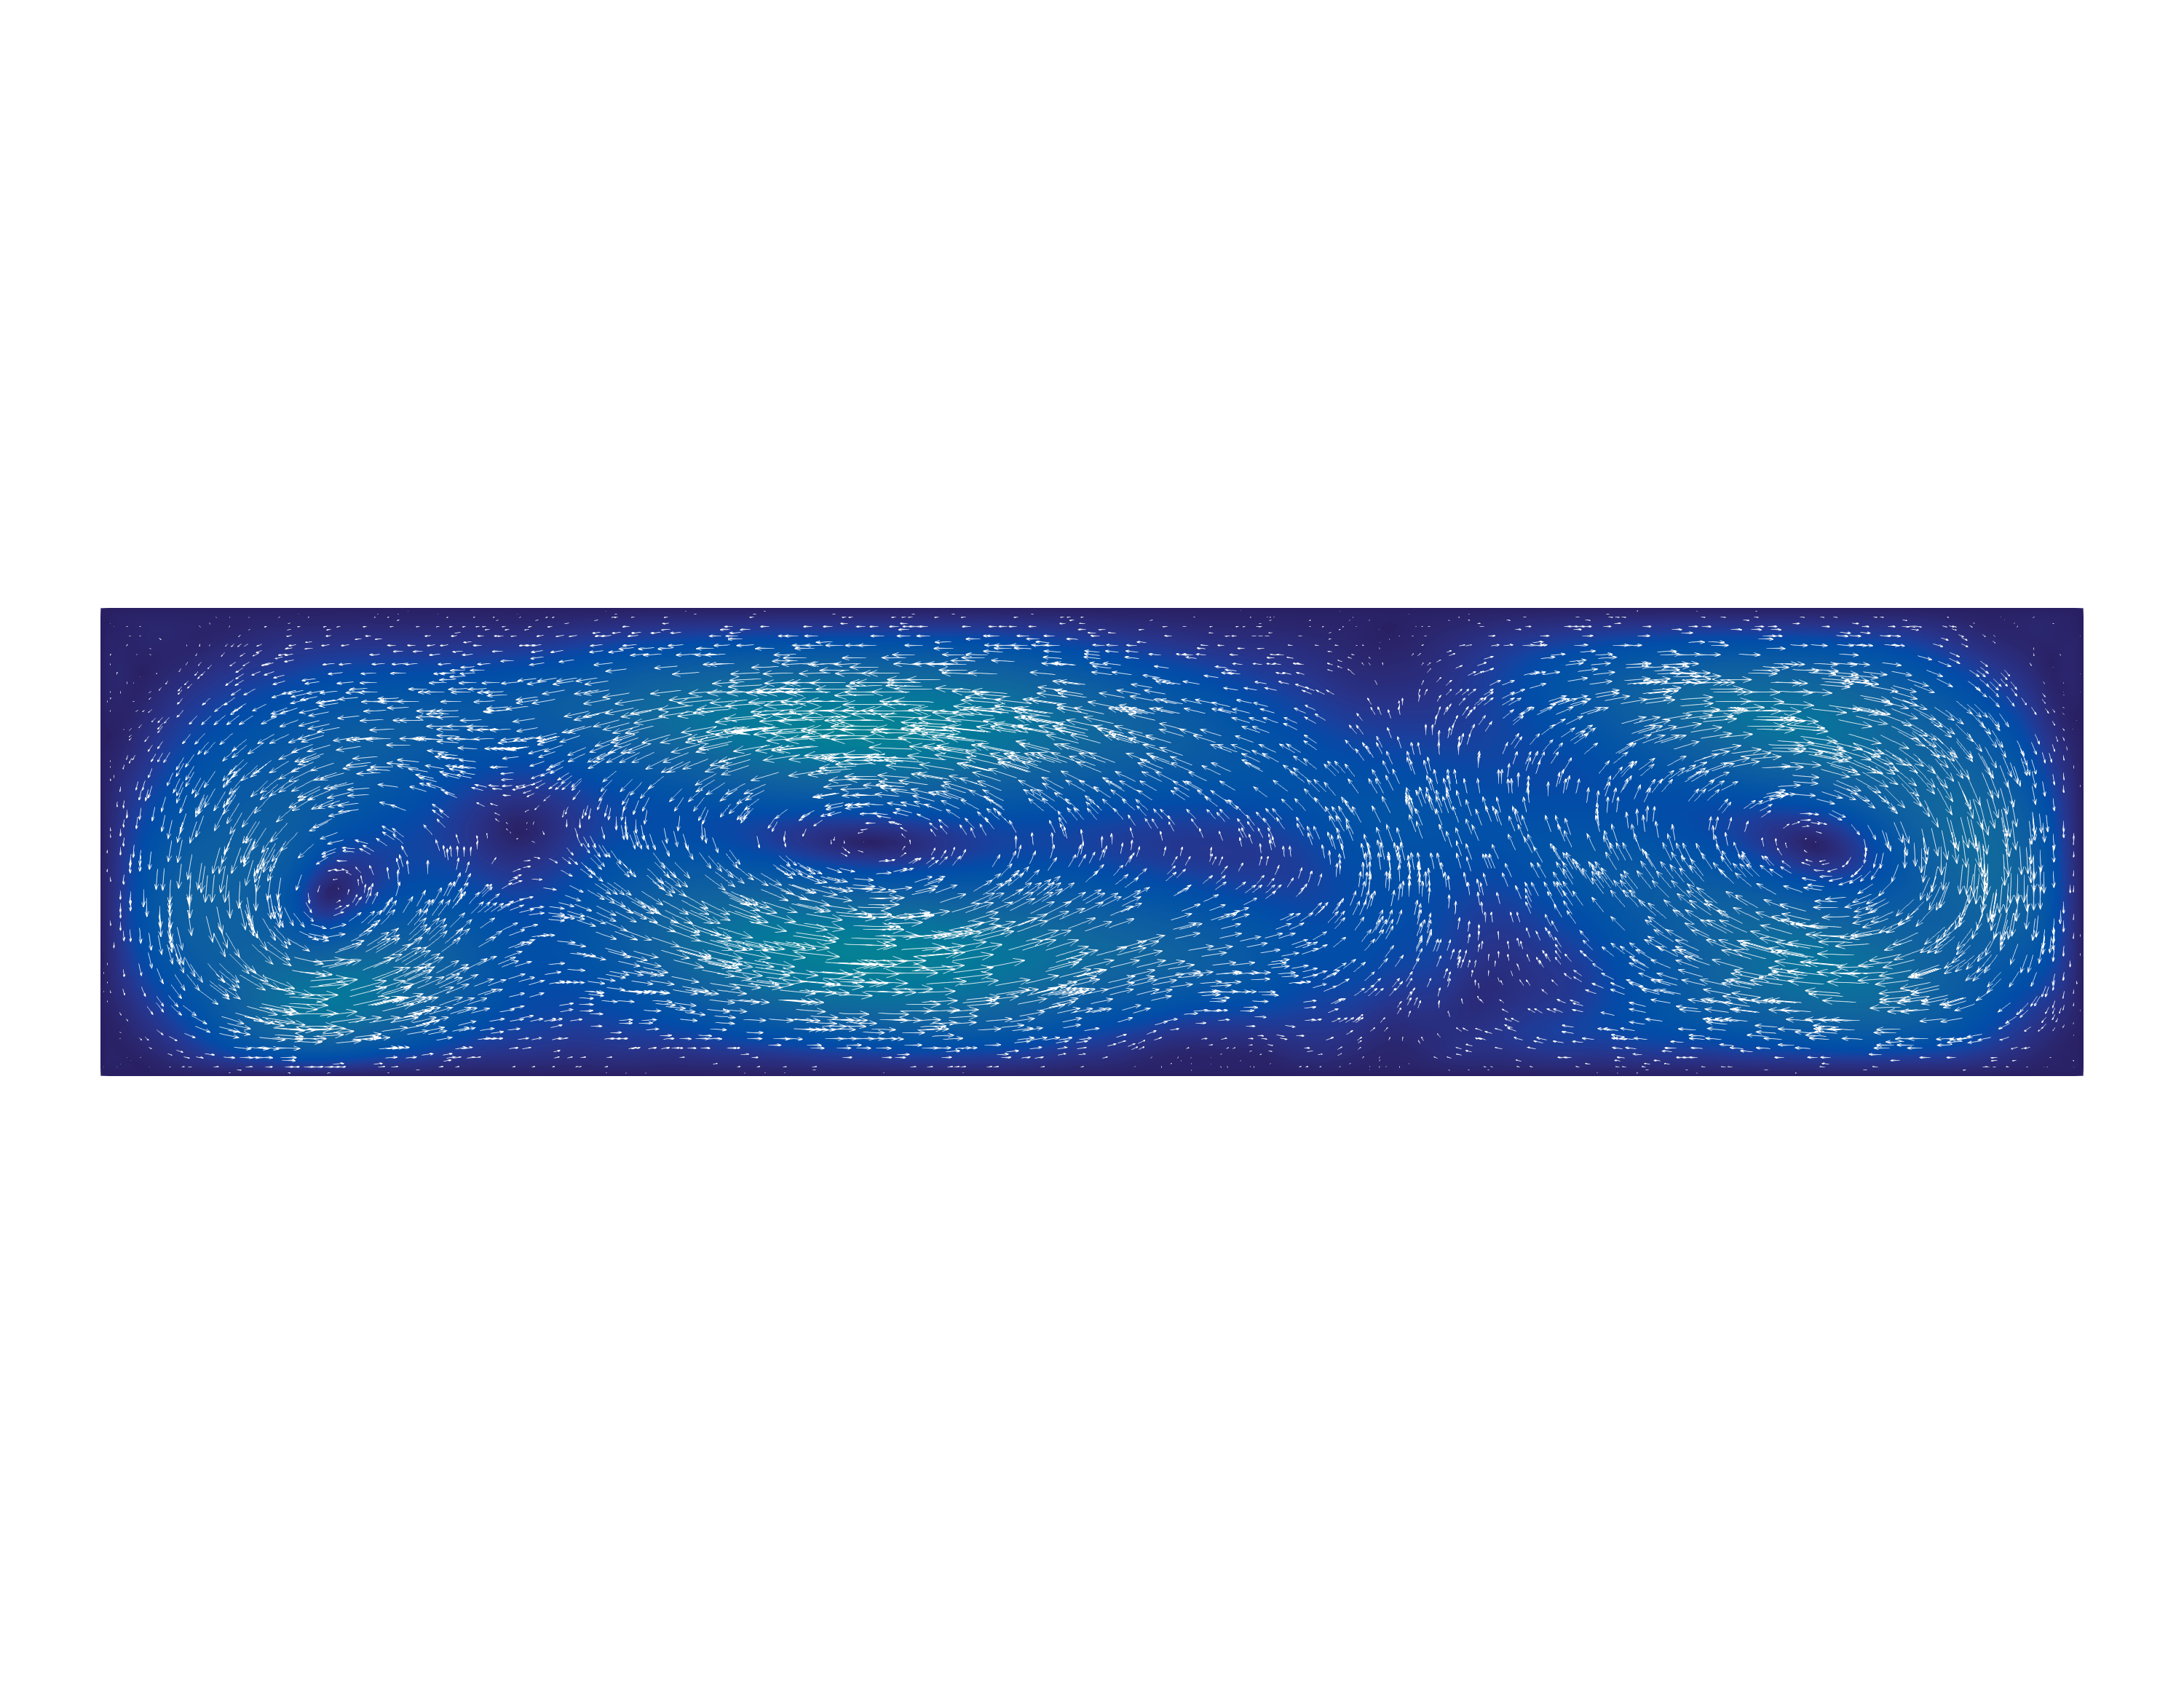
\includegraphics[width=0.9\textwidth]{../media/fourier/application/print/ab-0-2-velocity-harm.png}
        \caption{Anode $(1,2)$ désactivée}
        \label{fig:}
      \end{center}
    \end{subfigure}

    \begin{tikzpicture}
      \begin{axis}[
          colorbar,
          hide axis,
          scale only axis,
          height=0.10\textwidth,
          width=0.5\textwidth,
          colorbar horizontal,
          point meta min=0.0,
          point meta max=6.0,
          colorbar style={
            title=Vitesse $u_h$ [\si{\centi\meter\per\second}],
            width=4cm,
            height=0.3cm,
            xtick={0.0, 3.0, 6.0},
            at={(0.3\textwidth,0.4cm)},
            anchor=north
          }
        ]
        \addplot [] coordinates {(0,0)};
        \node (myfirstpic) at (0,0) {};
      \end{axis}
    \end{tikzpicture}

    \caption{Vitesse d'écoulement $u_h^\mathrm{S3D}$ dans l'ACD (haut)
      et $u_h^\mathrm{SF}$ sur une surface $x_3 = \thickness / 2$ à
      mi-hauteur dans le domaine $\Omega$ (bas).}

    \label{fig:harmonic-velocity-comp-a}
  \end{center}
\end{figure}


\begin{figure}[h!]
  \begin{center}
    \begin{subfigure}[t]{\textwidth}
      \begin{center}
        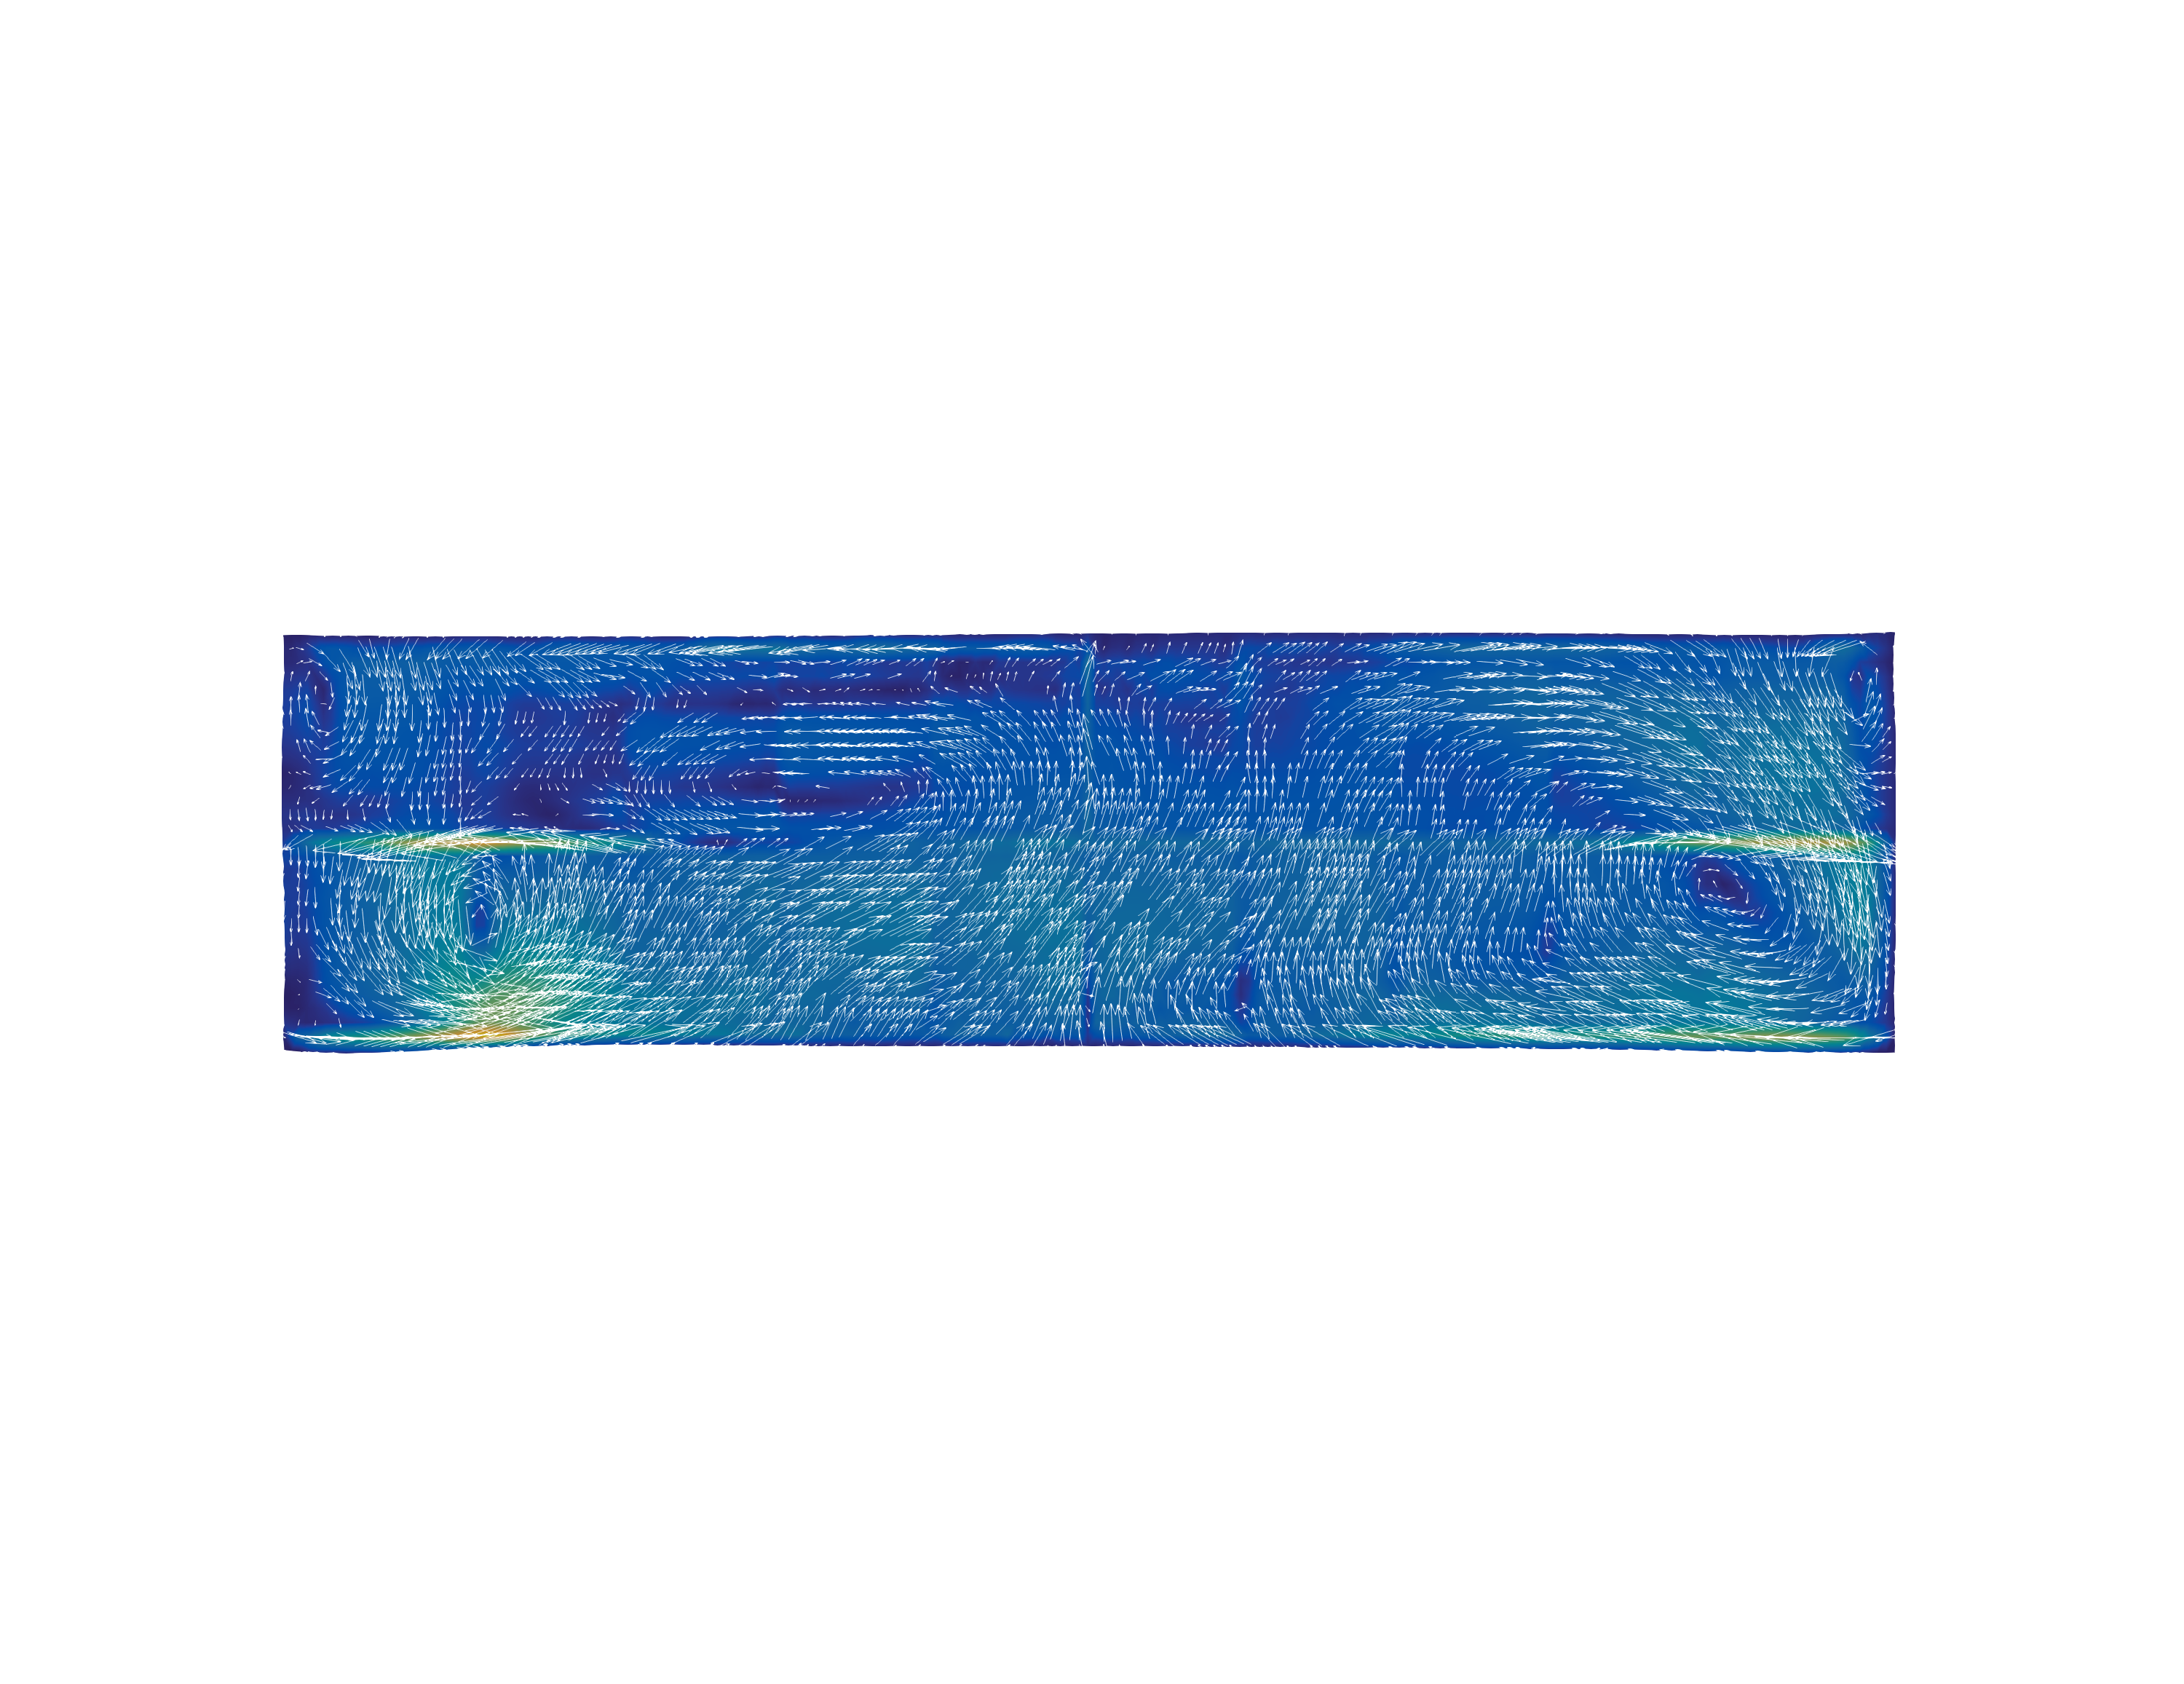
\includegraphics[width=0.9\textwidth]{../media/fourier/application/print/ab-1-1-velocity-acd.png}
        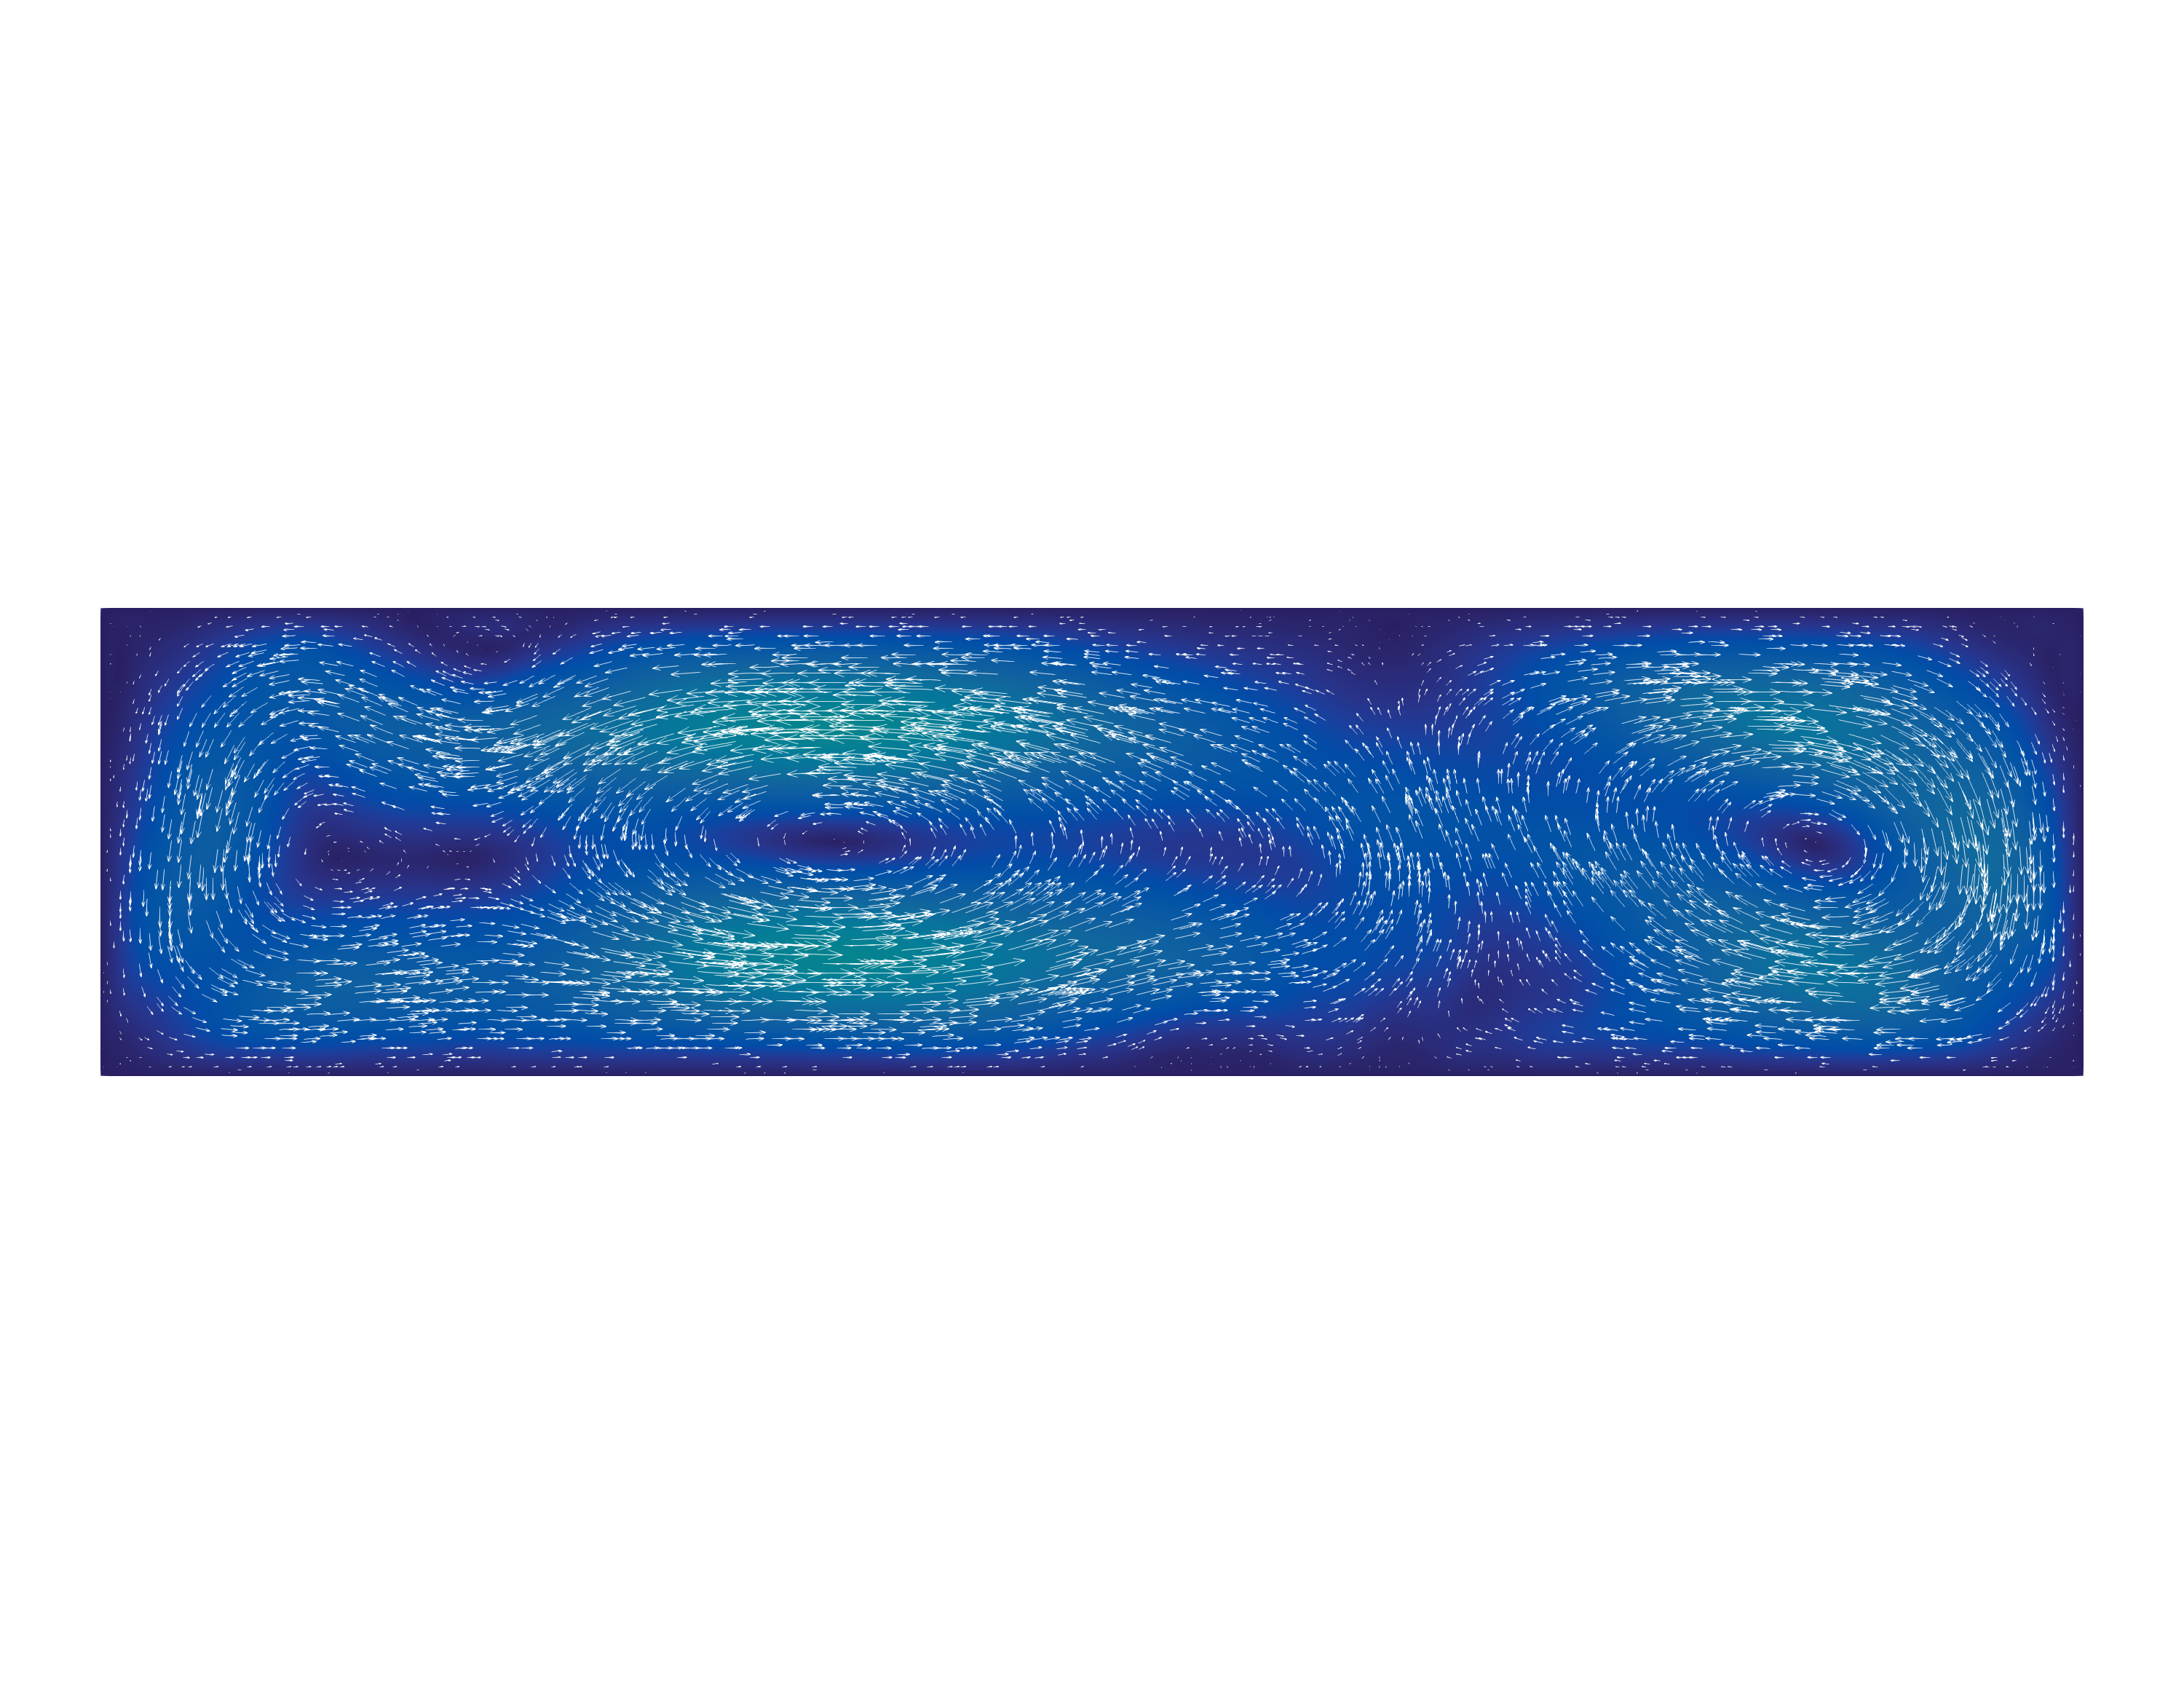
\includegraphics[width=0.9\textwidth]{../media/fourier/application/print/ab-1-1-velocity-harm.png}
        \caption{Anode $(2,1)$ désactivée}
        \label{fig:}
      \end{center}
    \end{subfigure}

    \begin{subfigure}[t]{\textwidth}
      \begin{center}
        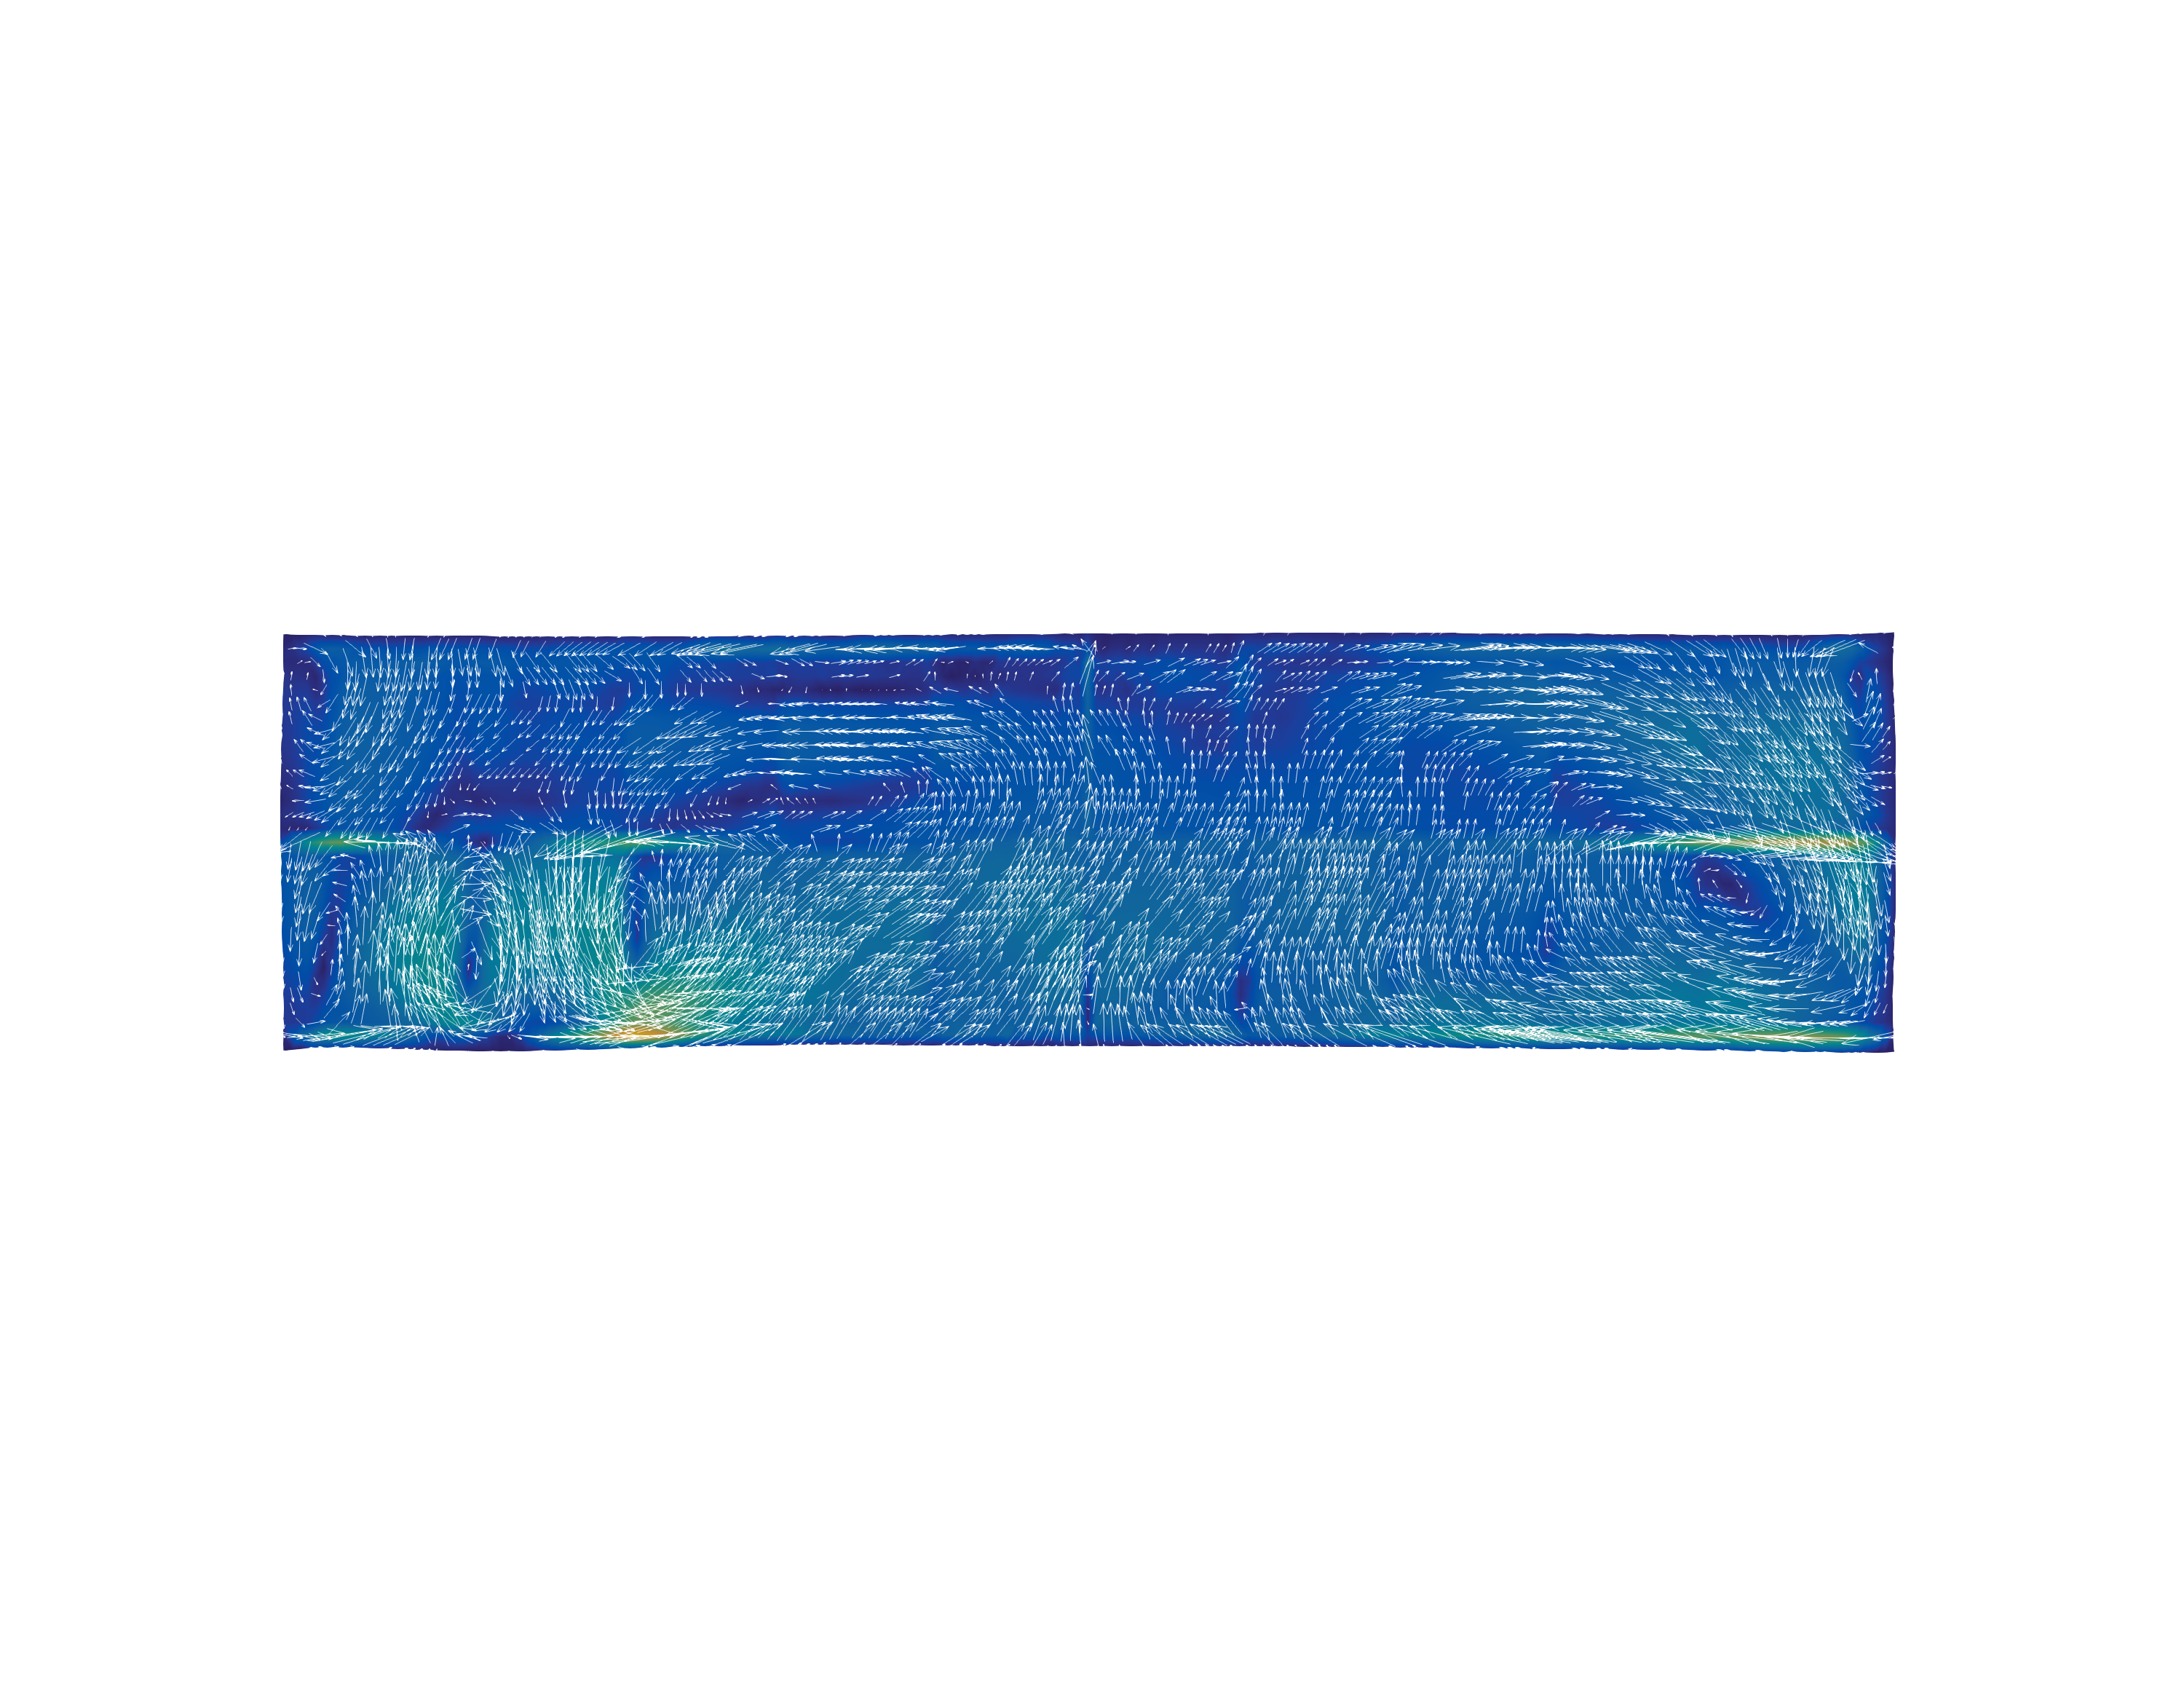
\includegraphics[width=0.9\textwidth]{../media/fourier/application/print/ab-1-2-velocity-acd.png}
        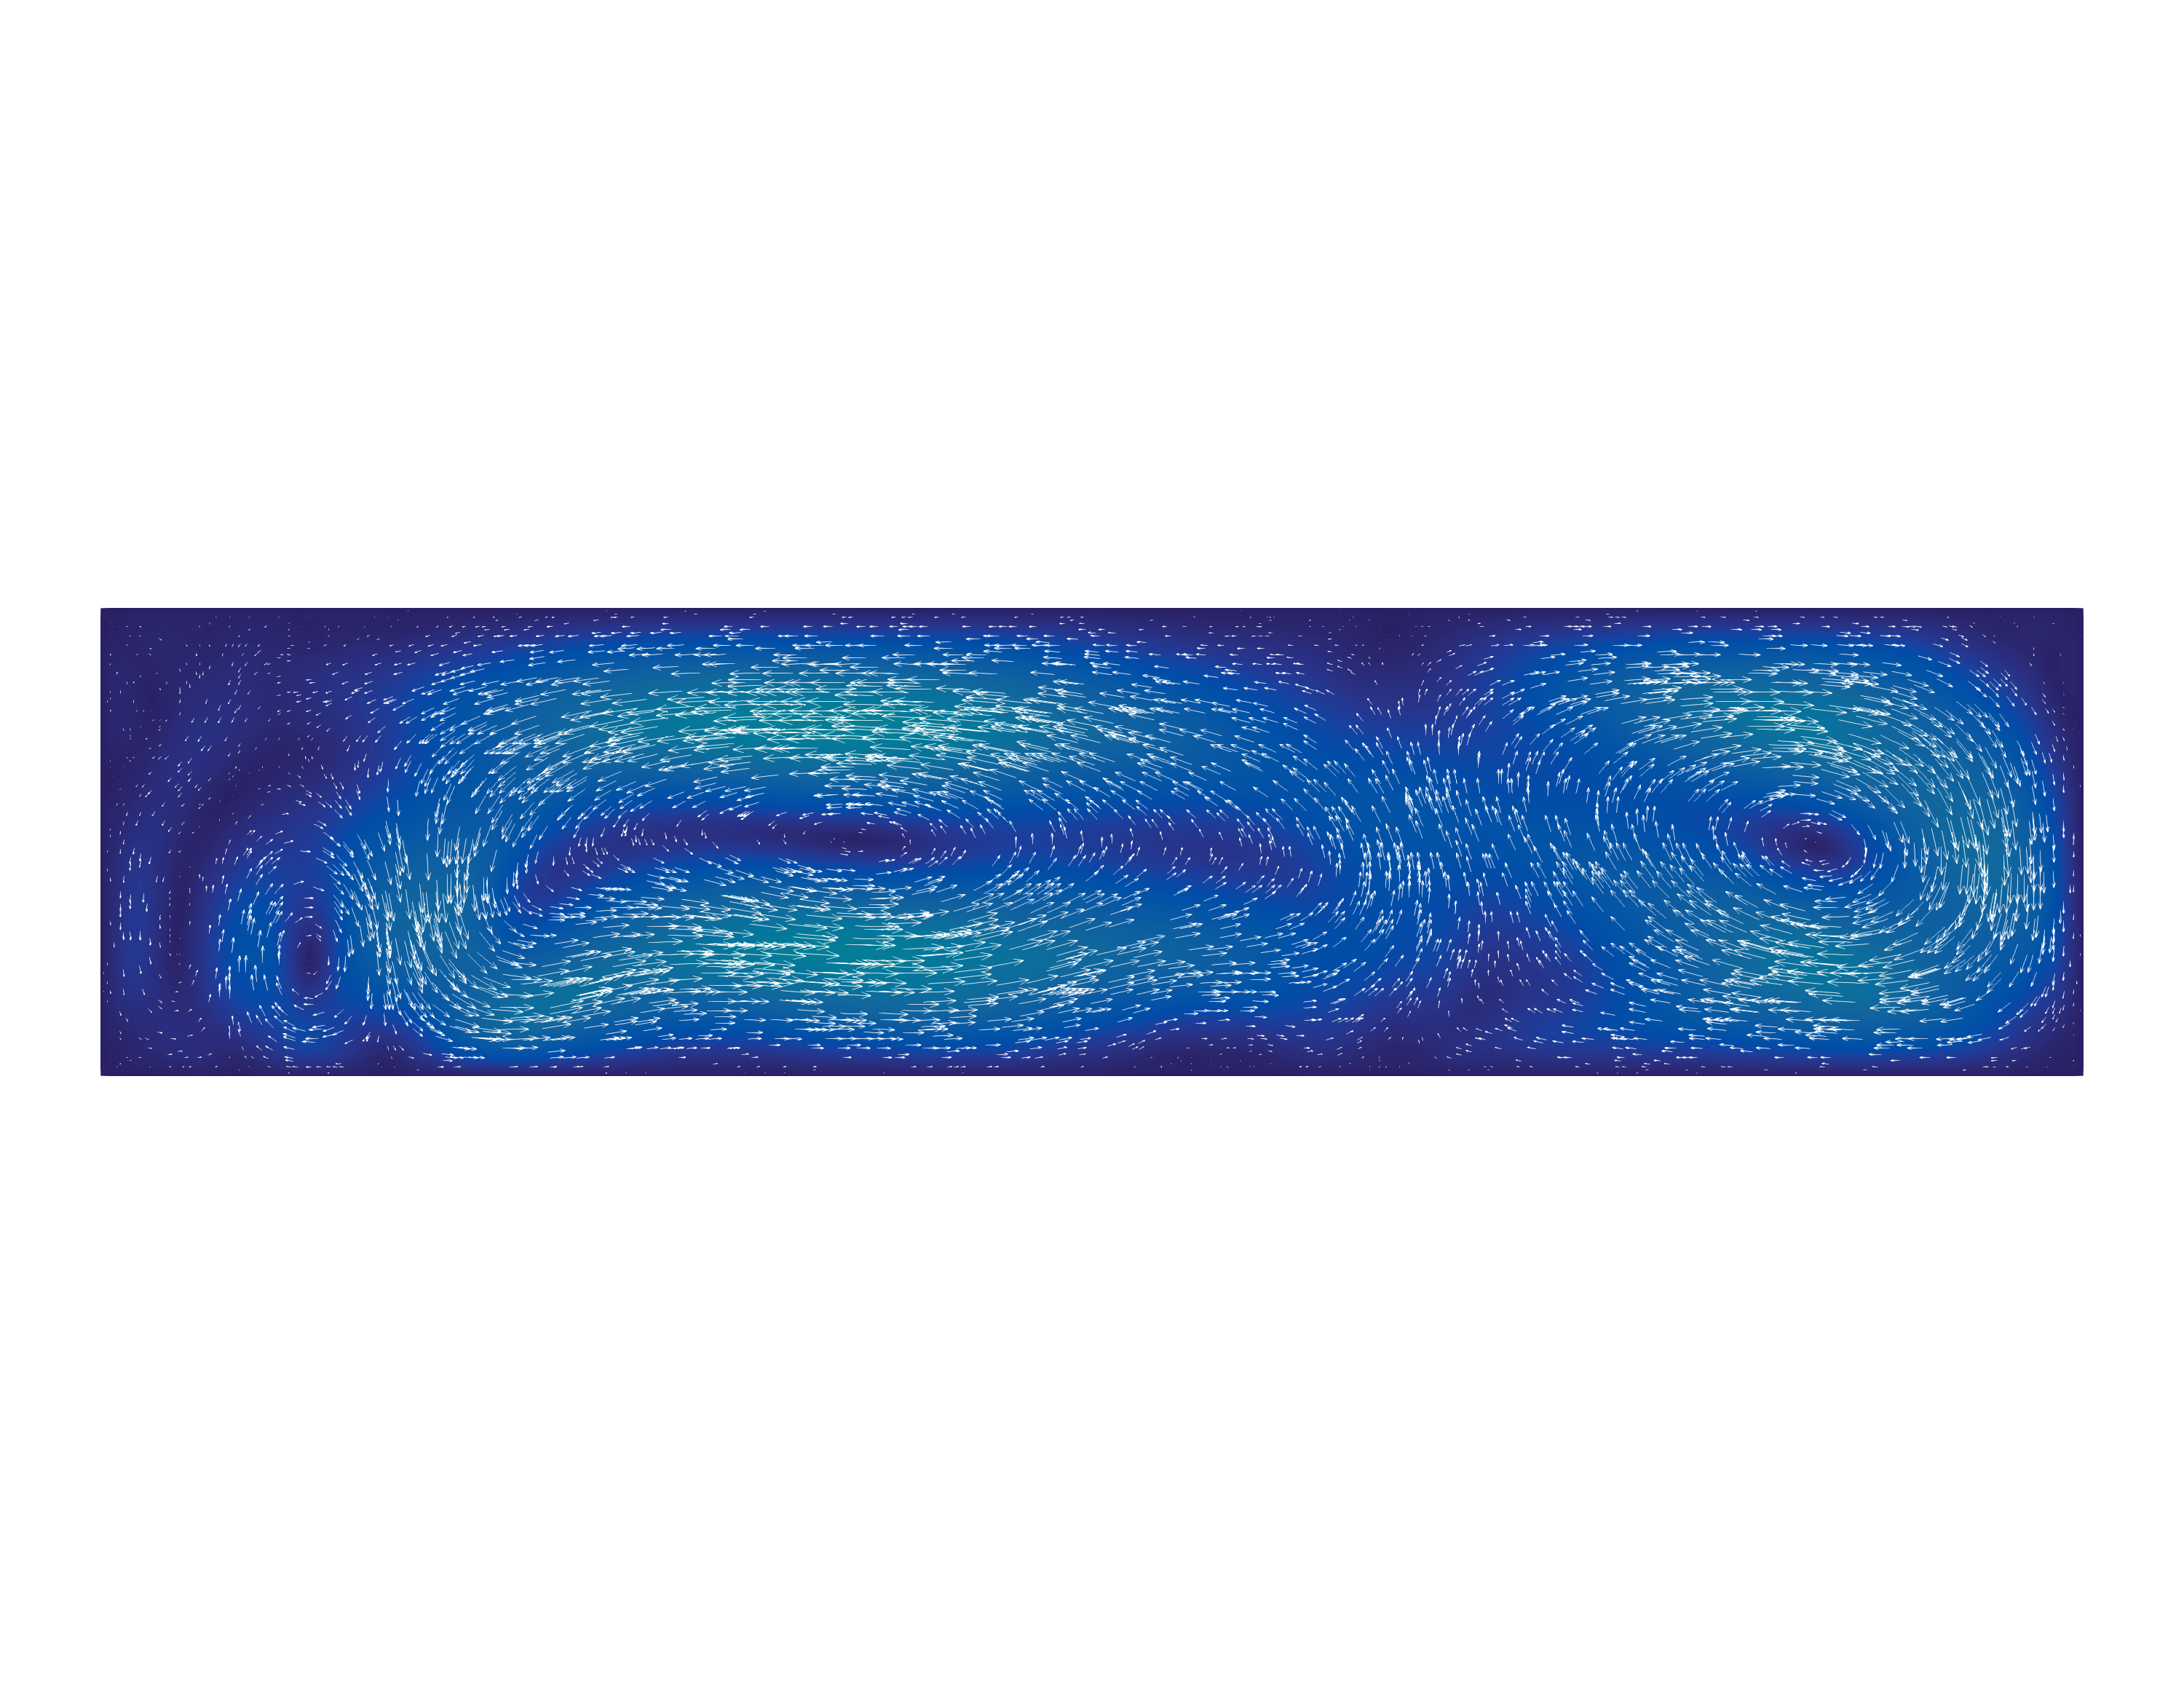
\includegraphics[width=0.9\textwidth]{../media/fourier/application/print/ab-1-2-velocity-harm.png}
        \caption{Anode $(2,2)$ désactivée}
        \label{fig:}
      \end{center}
    \end{subfigure}

    \begin{tikzpicture}
      \begin{axis}[
          colorbar,
          hide axis,
          scale only axis,
          height=0.10\textwidth,
          width=0.5\textwidth,
          colorbar horizontal,
          point meta min=0.0,
          point meta max=6.0,
          colorbar style={
            title=Vitesse $u_h$ [\si{\centi\meter\per\second}],
            width=4cm,
            height=0.3cm,
            xtick={0.0, 3.0, 6.0},
            at={(0.3\textwidth,0.4cm)},
            anchor=north
          }
        ]
        \addplot [] coordinates {(0,0)};
        \node (myfirstpic) at (0,0) {};
      \end{axis}
    \end{tikzpicture}

    \caption{Vitesse d'écoulement $u_h^\mathrm{S3D}$ dans l'ACD (haut)
      et $u_h^\mathrm{SF}$ sur une surface $x_3 = \thickness / 2$ à
      mi-hauteur dans le domaine $\Omega$ (bas).}

    \label{fig:harmonic-velocity-comp-b}
  \end{center}
\end{figure}

\begin{figure}[h!]
  \begin{center}
    \begin{subfigure}[t]{\textwidth}
      \begin{center}
        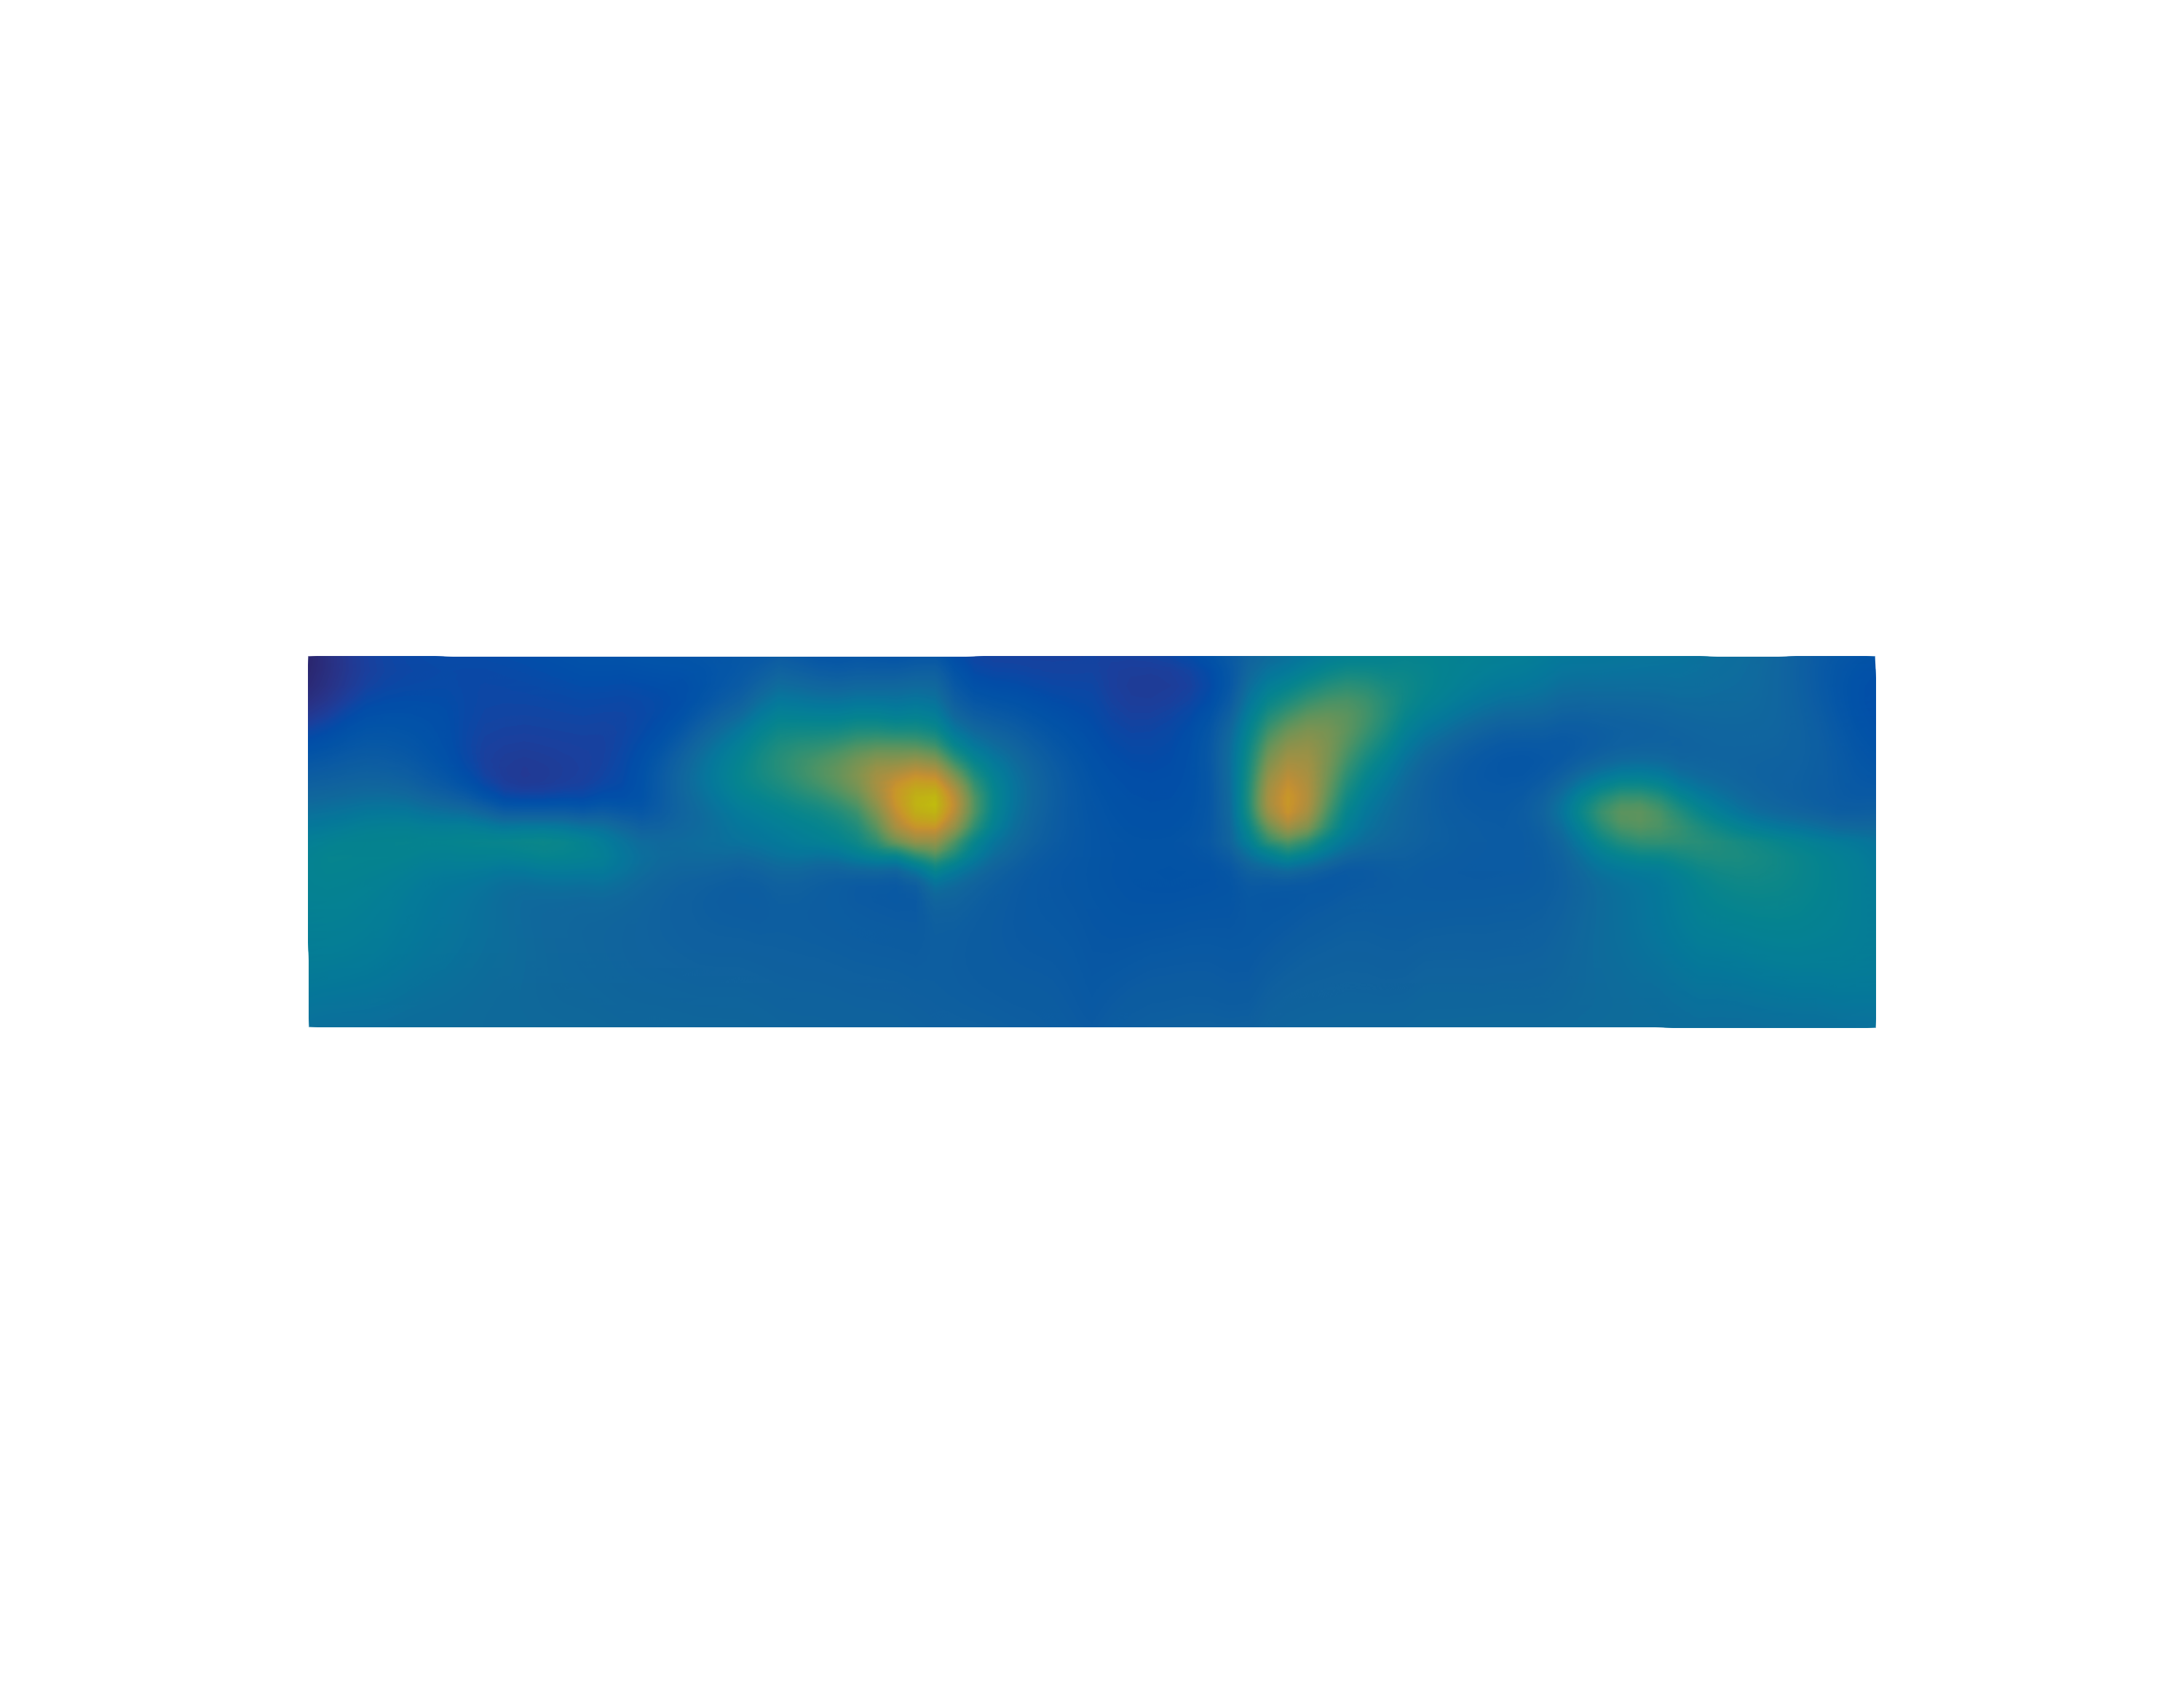
\includegraphics[width=0.99\textwidth]{../media/fourier/application/print/ab-0-1-concentration-acd.png}
        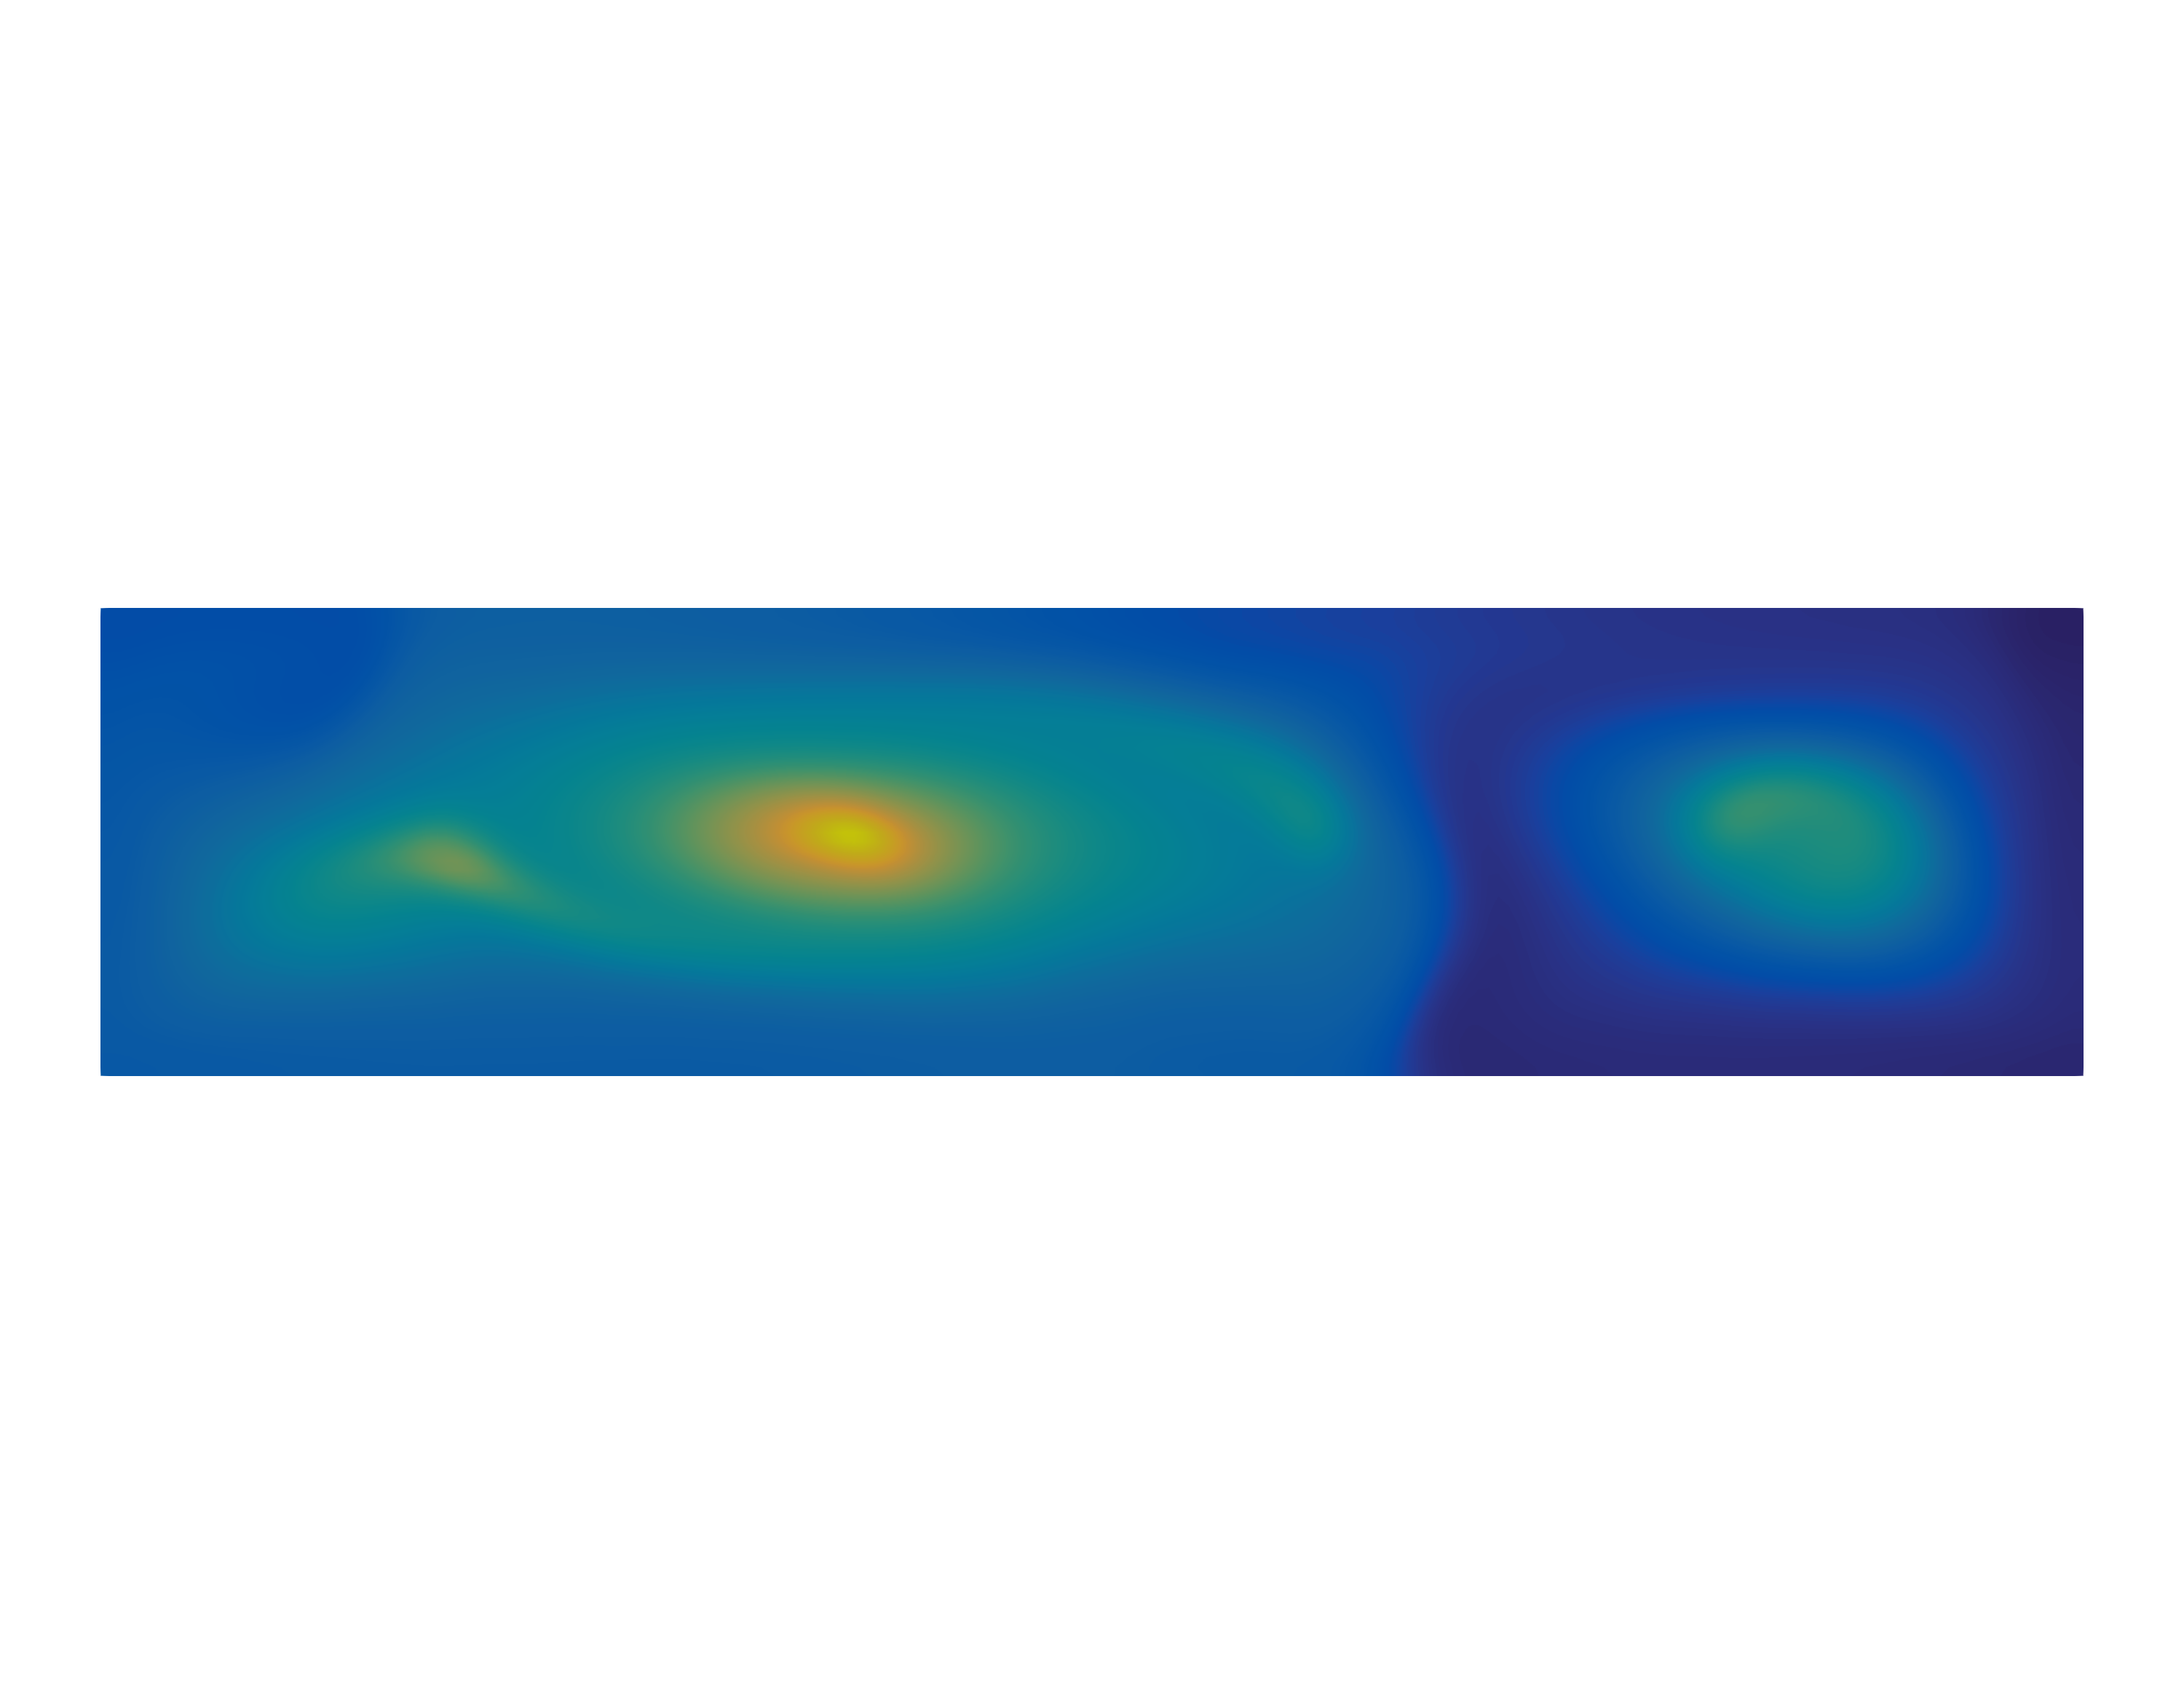
\includegraphics[width=0.99\textwidth]{../media/fourier/application/print/ab-0-1-concentration-harm.png}
        \caption{Anode $(1,1)$ désactivée}
        \label{fig:}
      \end{center}
    \end{subfigure}

    \begin{subfigure}[t]{\textwidth}
      \begin{center}
        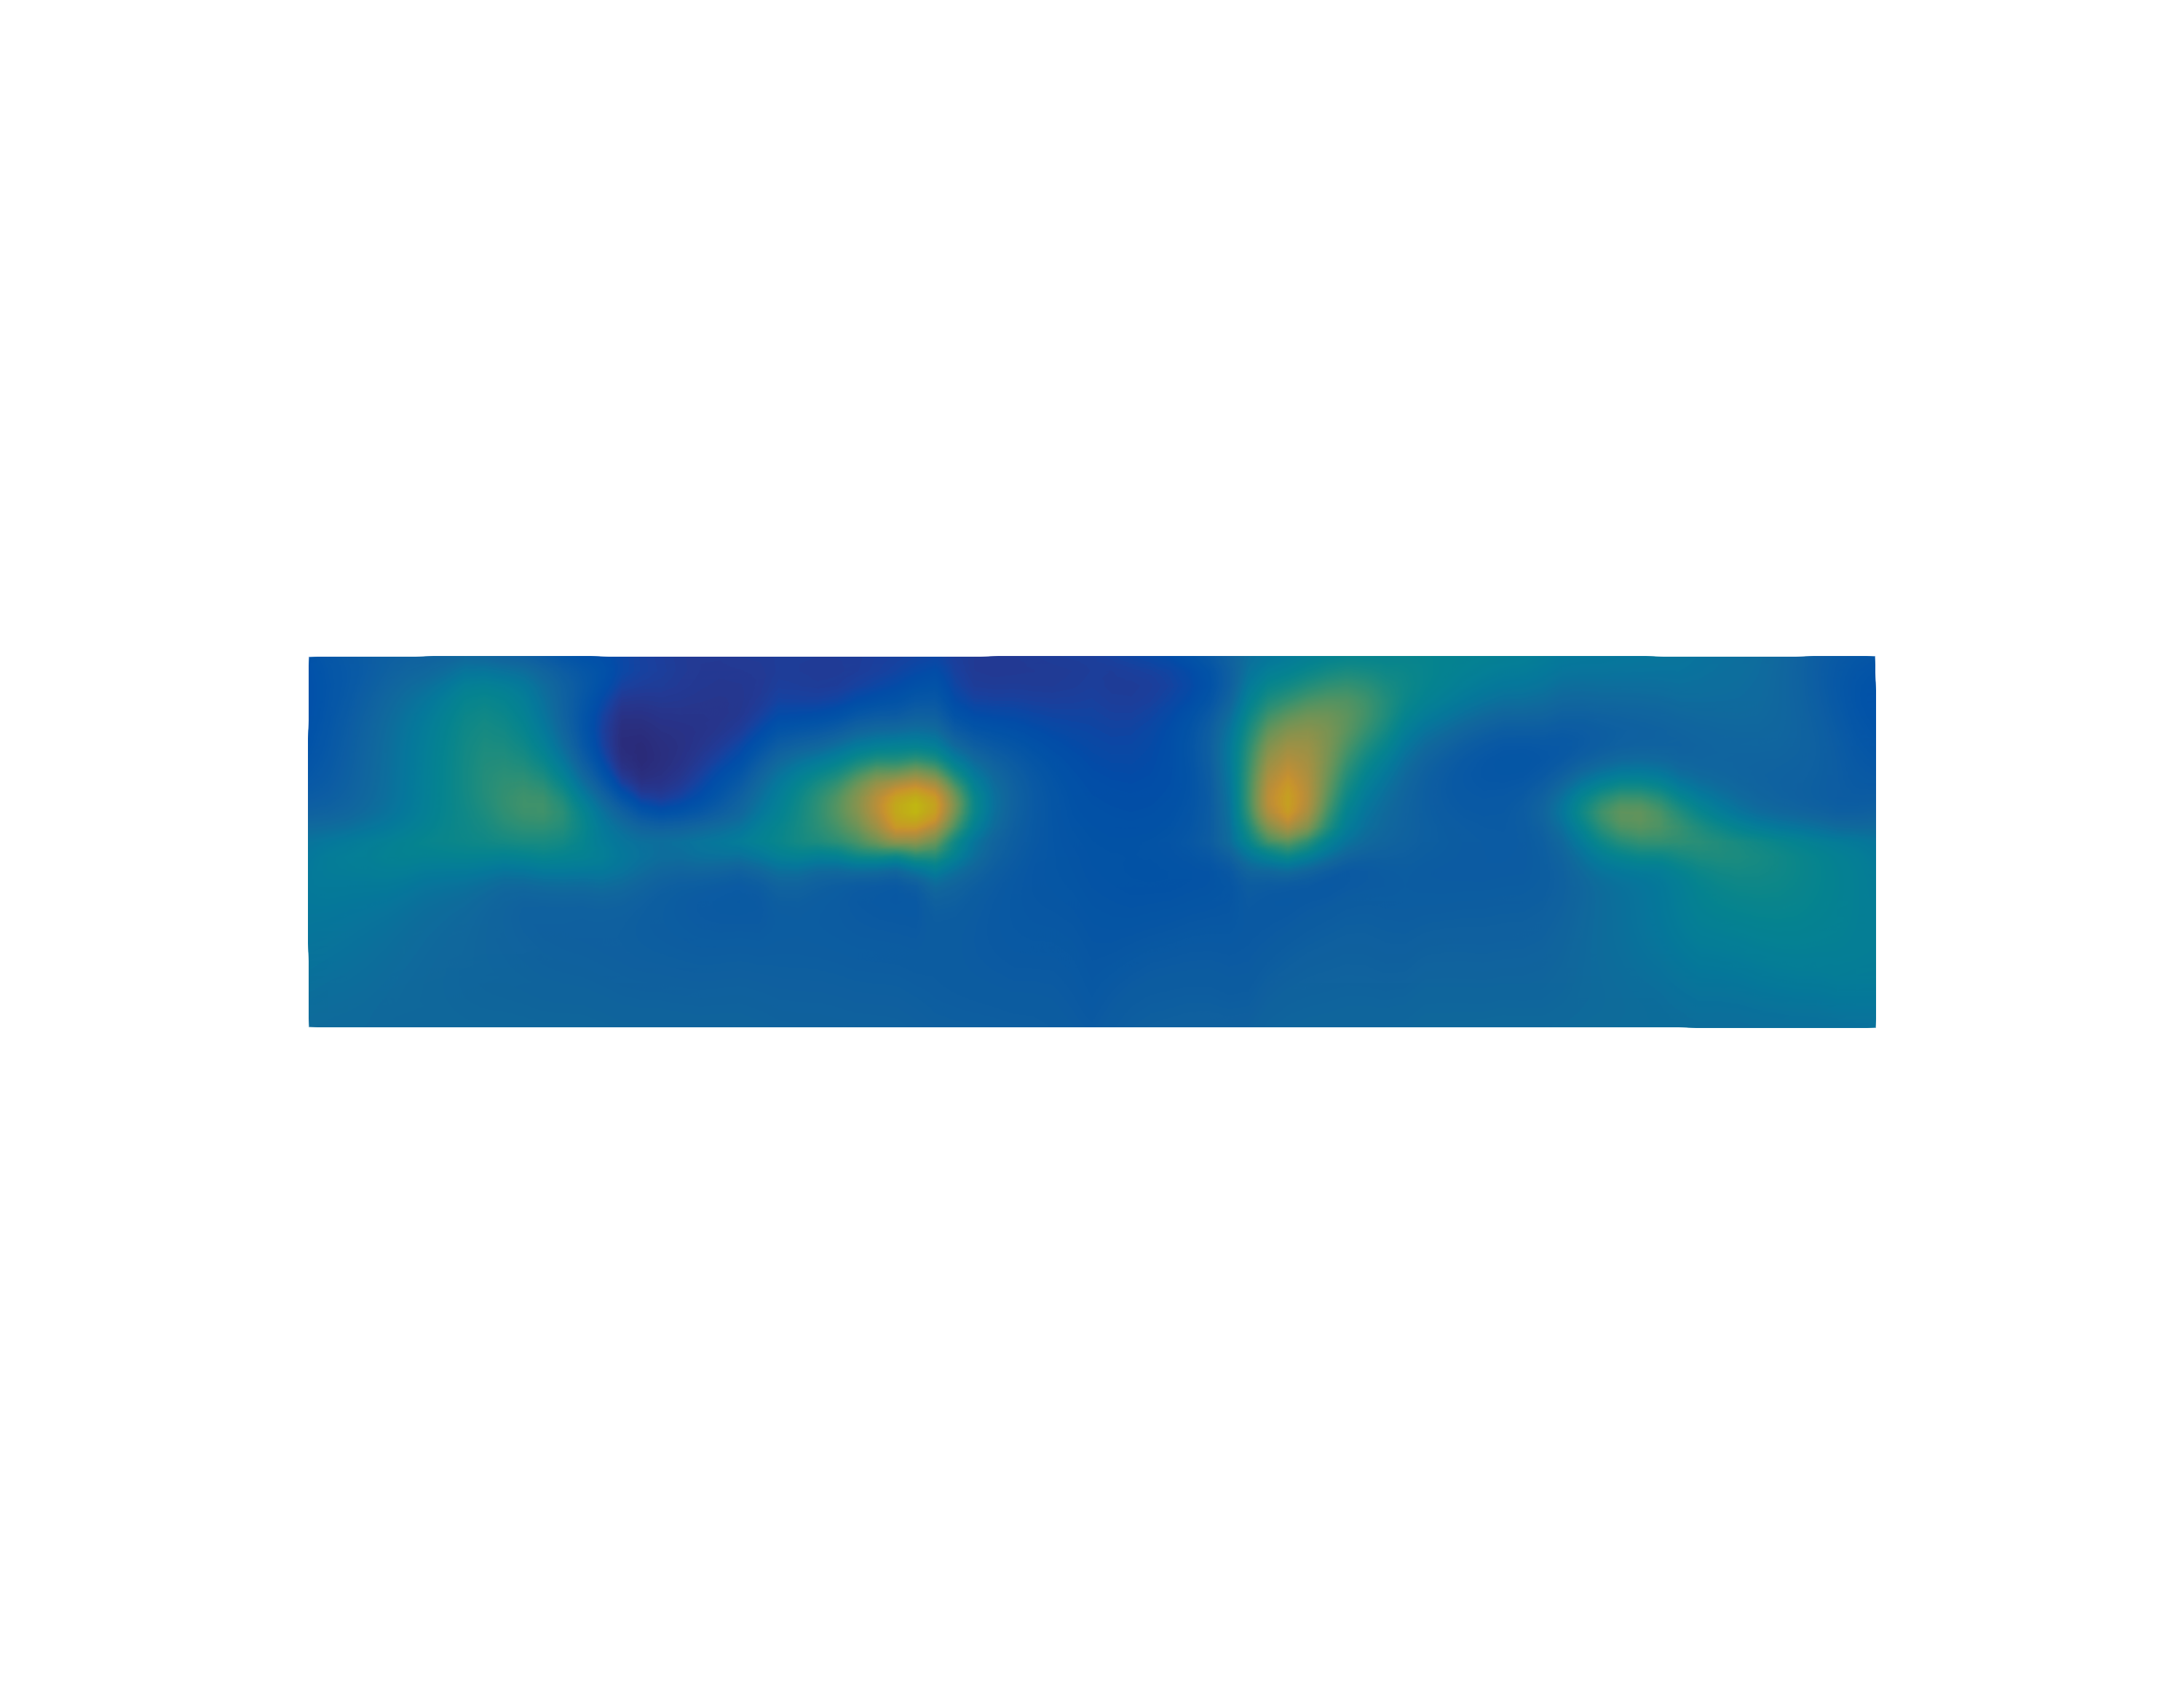
\includegraphics[width=0.99\textwidth]{../media/fourier/application/print/ab-0-2-concentration-acd.png}
        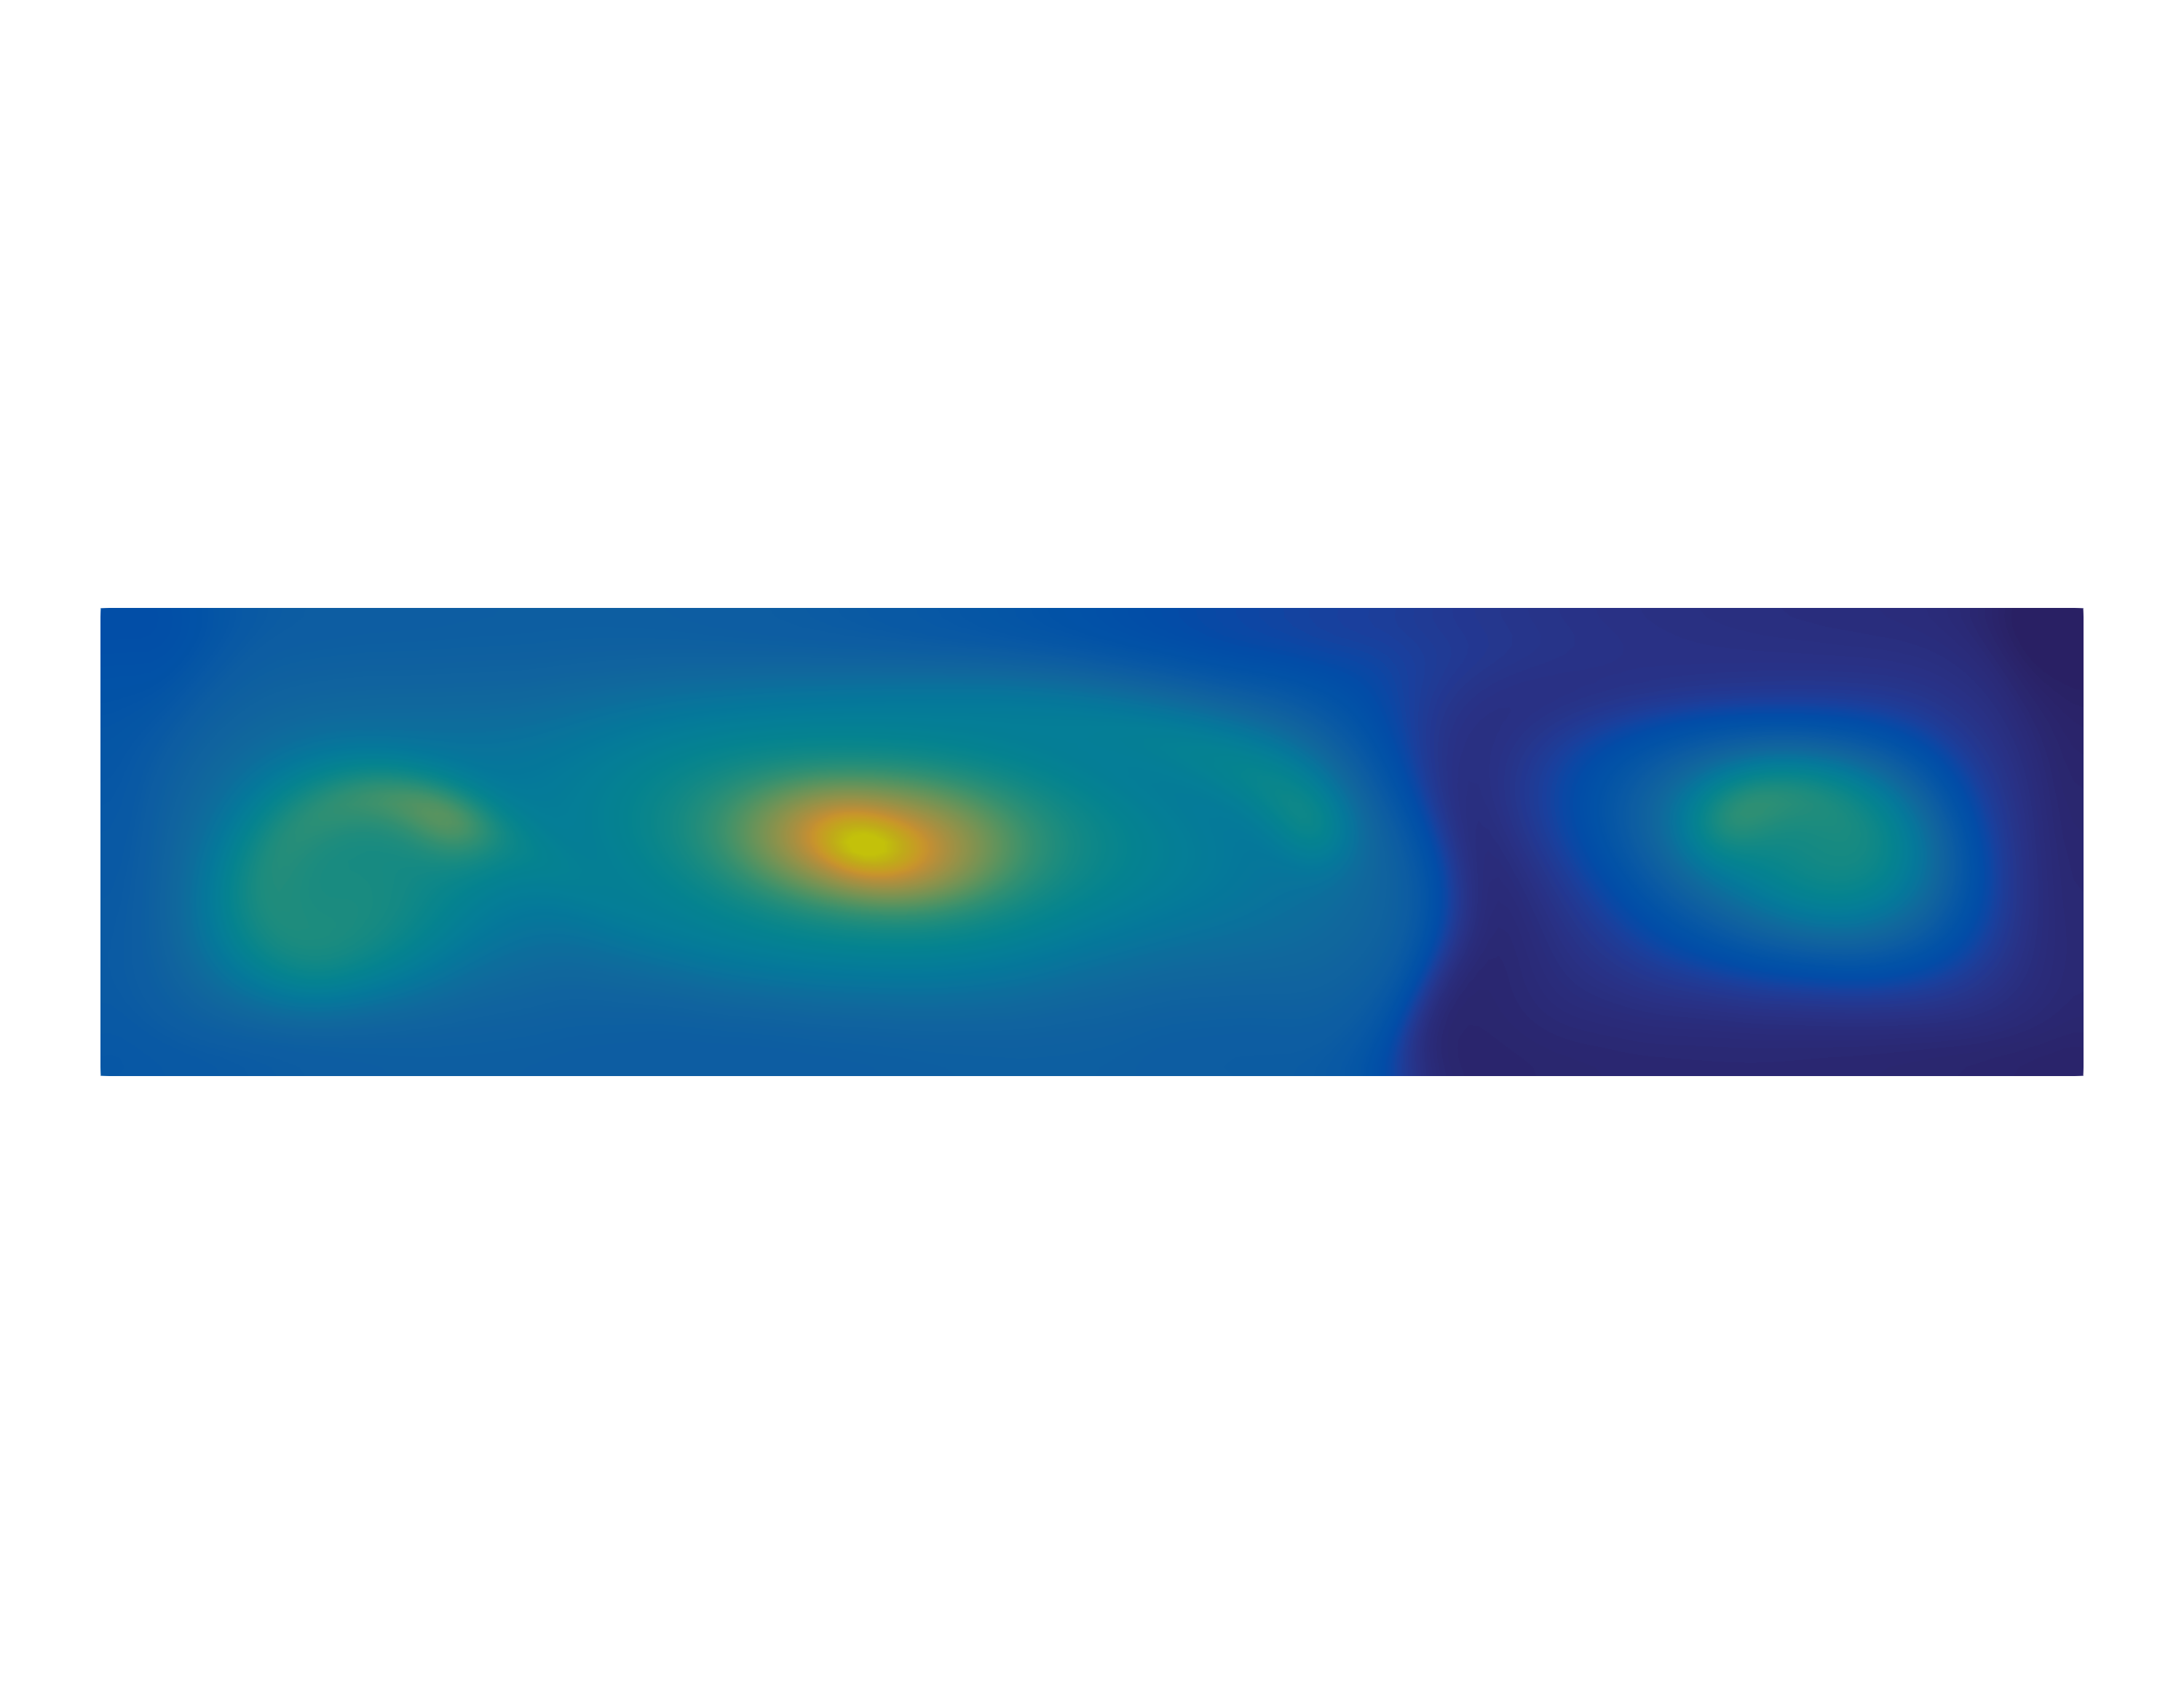
\includegraphics[width=0.99\textwidth]{../media/fourier/application/print/ab-0-2-concentration-harm.png}
        \caption{Anode $(1,2)$ désactivée}
        \label{fig:}
      \end{center}
    \end{subfigure}

    \begin{tikzpicture}
      \begin{axis}[
          colorbar,
          hide axis,
          scale only axis,
          height=0.1\textwidth,
          width=0.5\textwidth,
          colorbar horizontal,
          point meta min=1.73,
          point meta max=6.84,
          colorbar style={
            title=Concentration $c$ [w\%],
            width=4cm,
            height=0.3cm,
            xtick={1.73, 3.0, 5.0, 6.84},
            at={(0.5\textwidth,0.4cm)},
            anchor=north
          }
        ]
        \addplot [] coordinates {(0,0)};
        \node (myfirstpic) at (0,0) {};
      \end{axis}
    \end{tikzpicture}

    \caption{Champ de concentration $c^\mathrm{S3D}$ (haut) et
      $c^\mathrm{SF}$ dans les différentes configurations anodiques.}

    \label{fig:harmonic-concentration-comp-a}
  \end{center}
\end{figure}

\begin{figure}[h!]
  \begin{center}
    \begin{subfigure}[t]{\textwidth}
      \begin{center}
        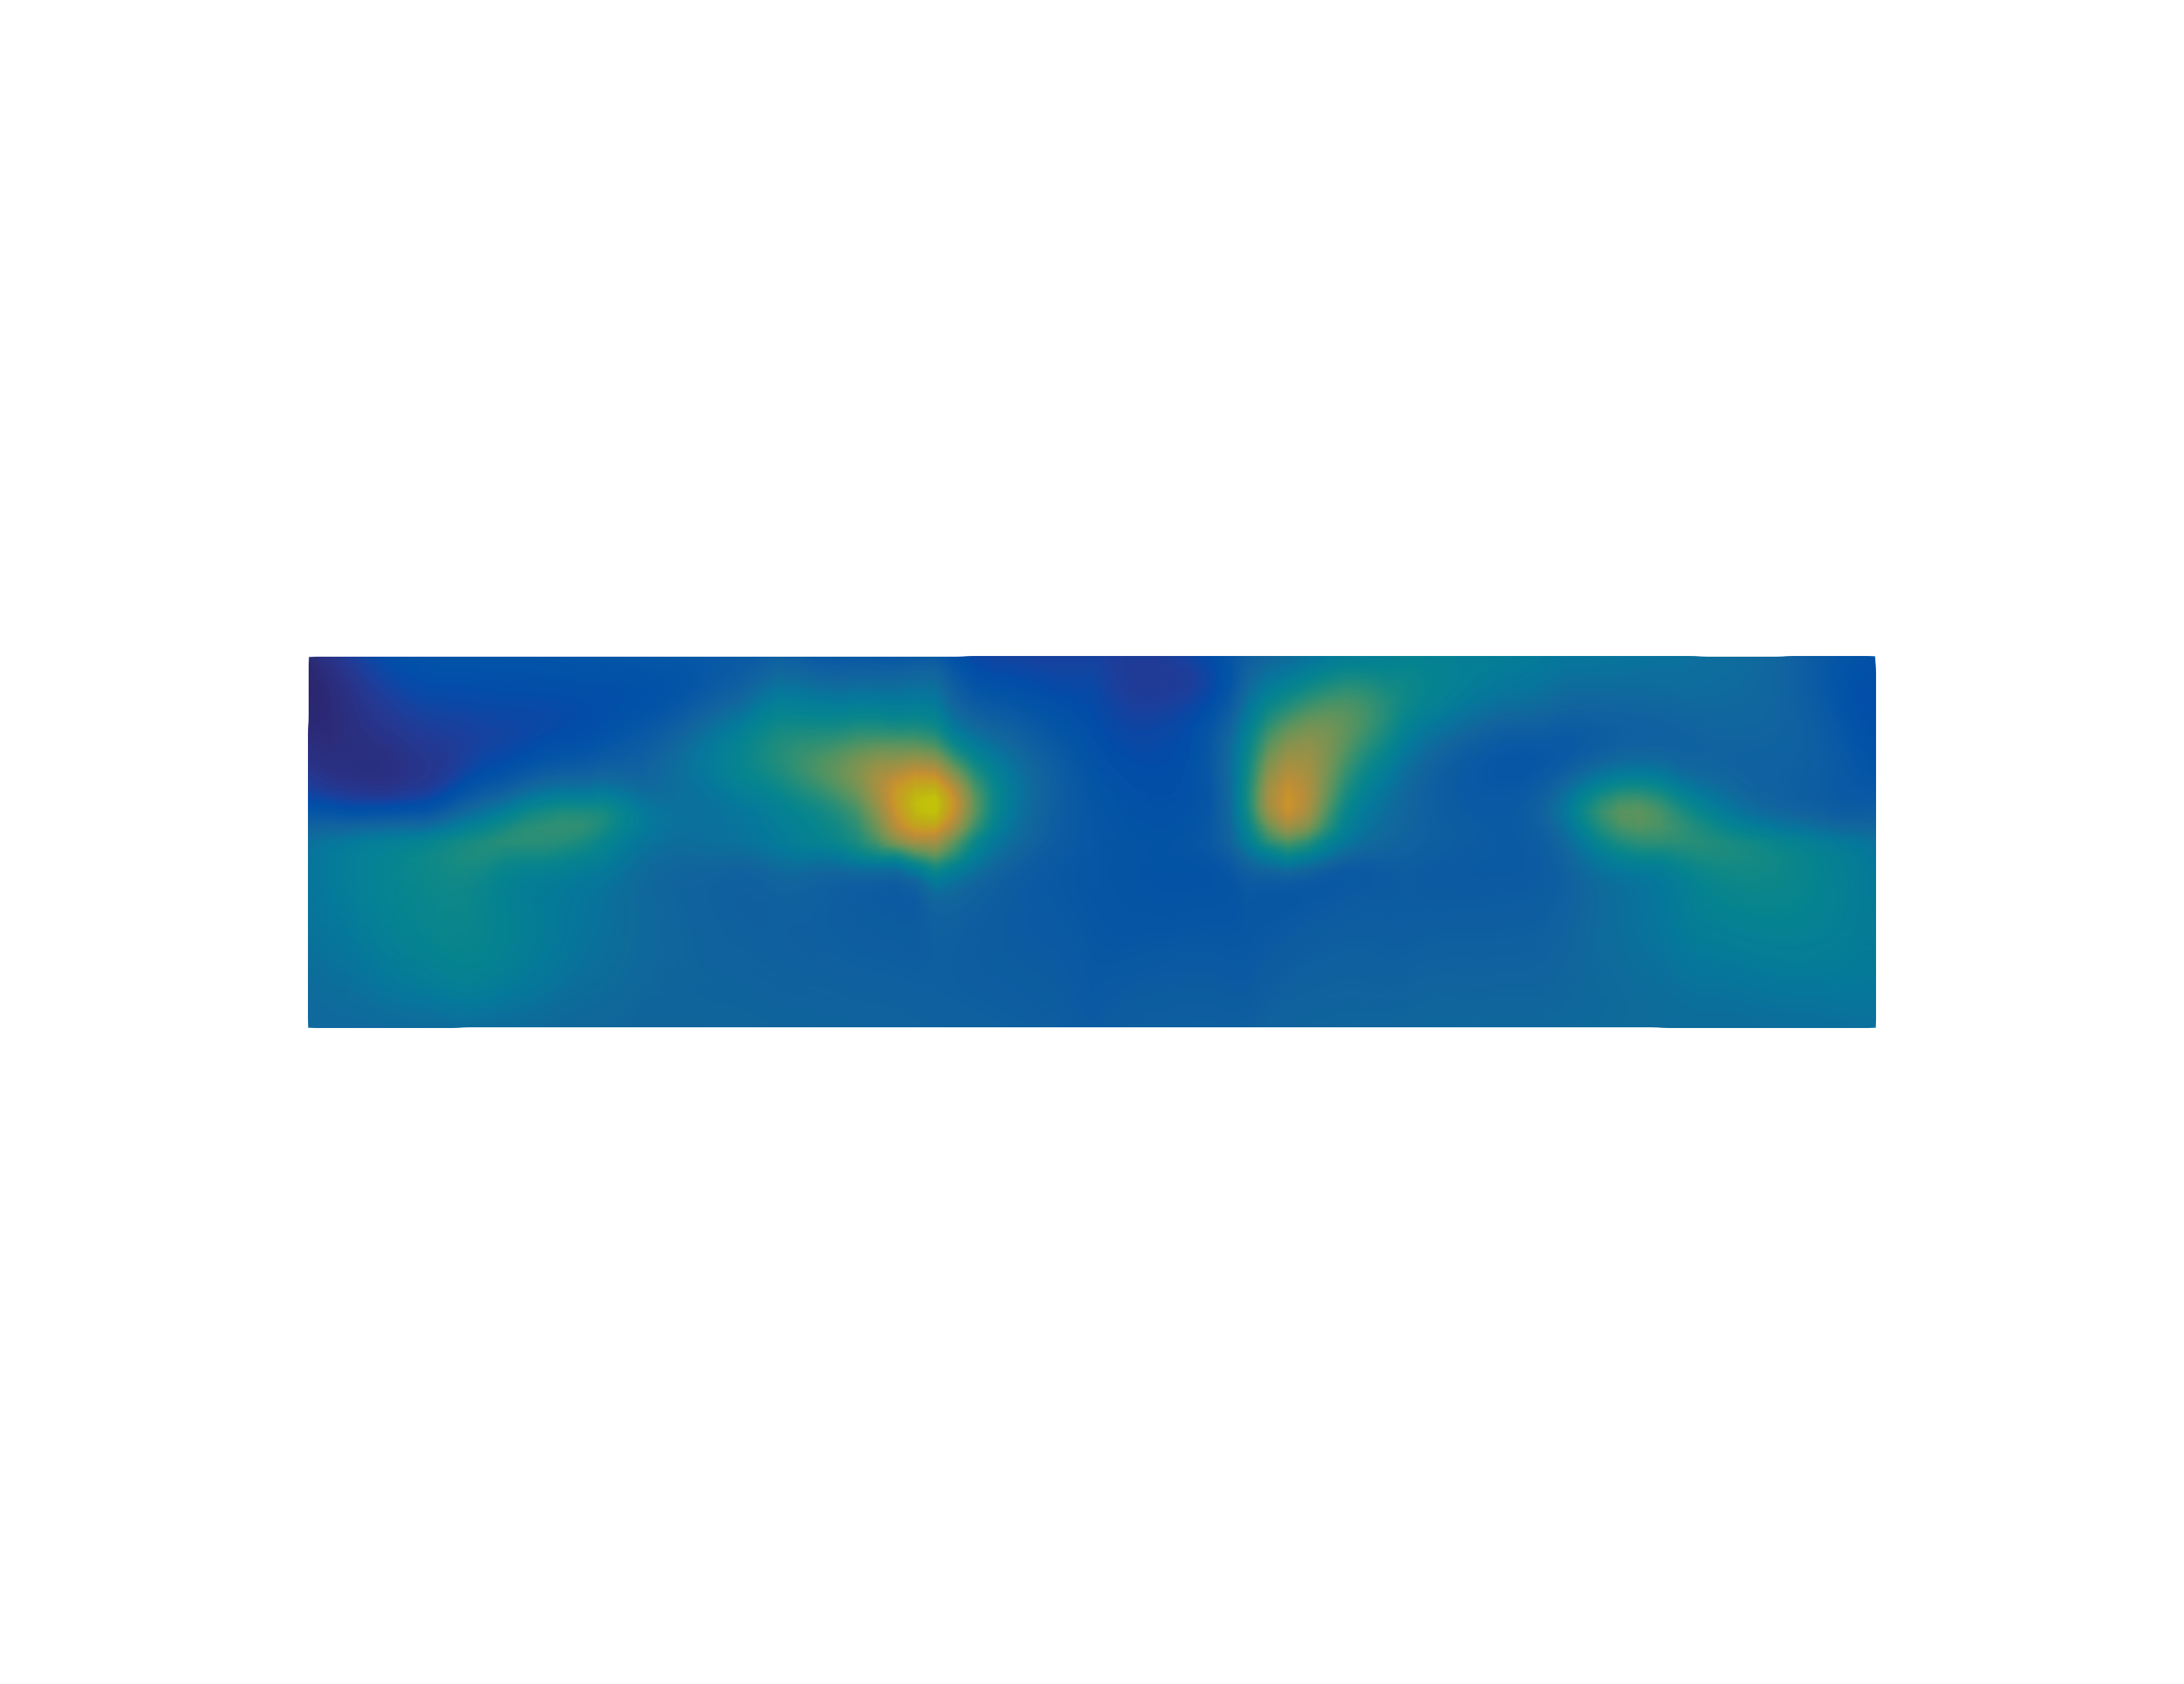
\includegraphics[width=0.99\textwidth]{../media/fourier/application/print/ab-1-1-concentration-acd.png}
        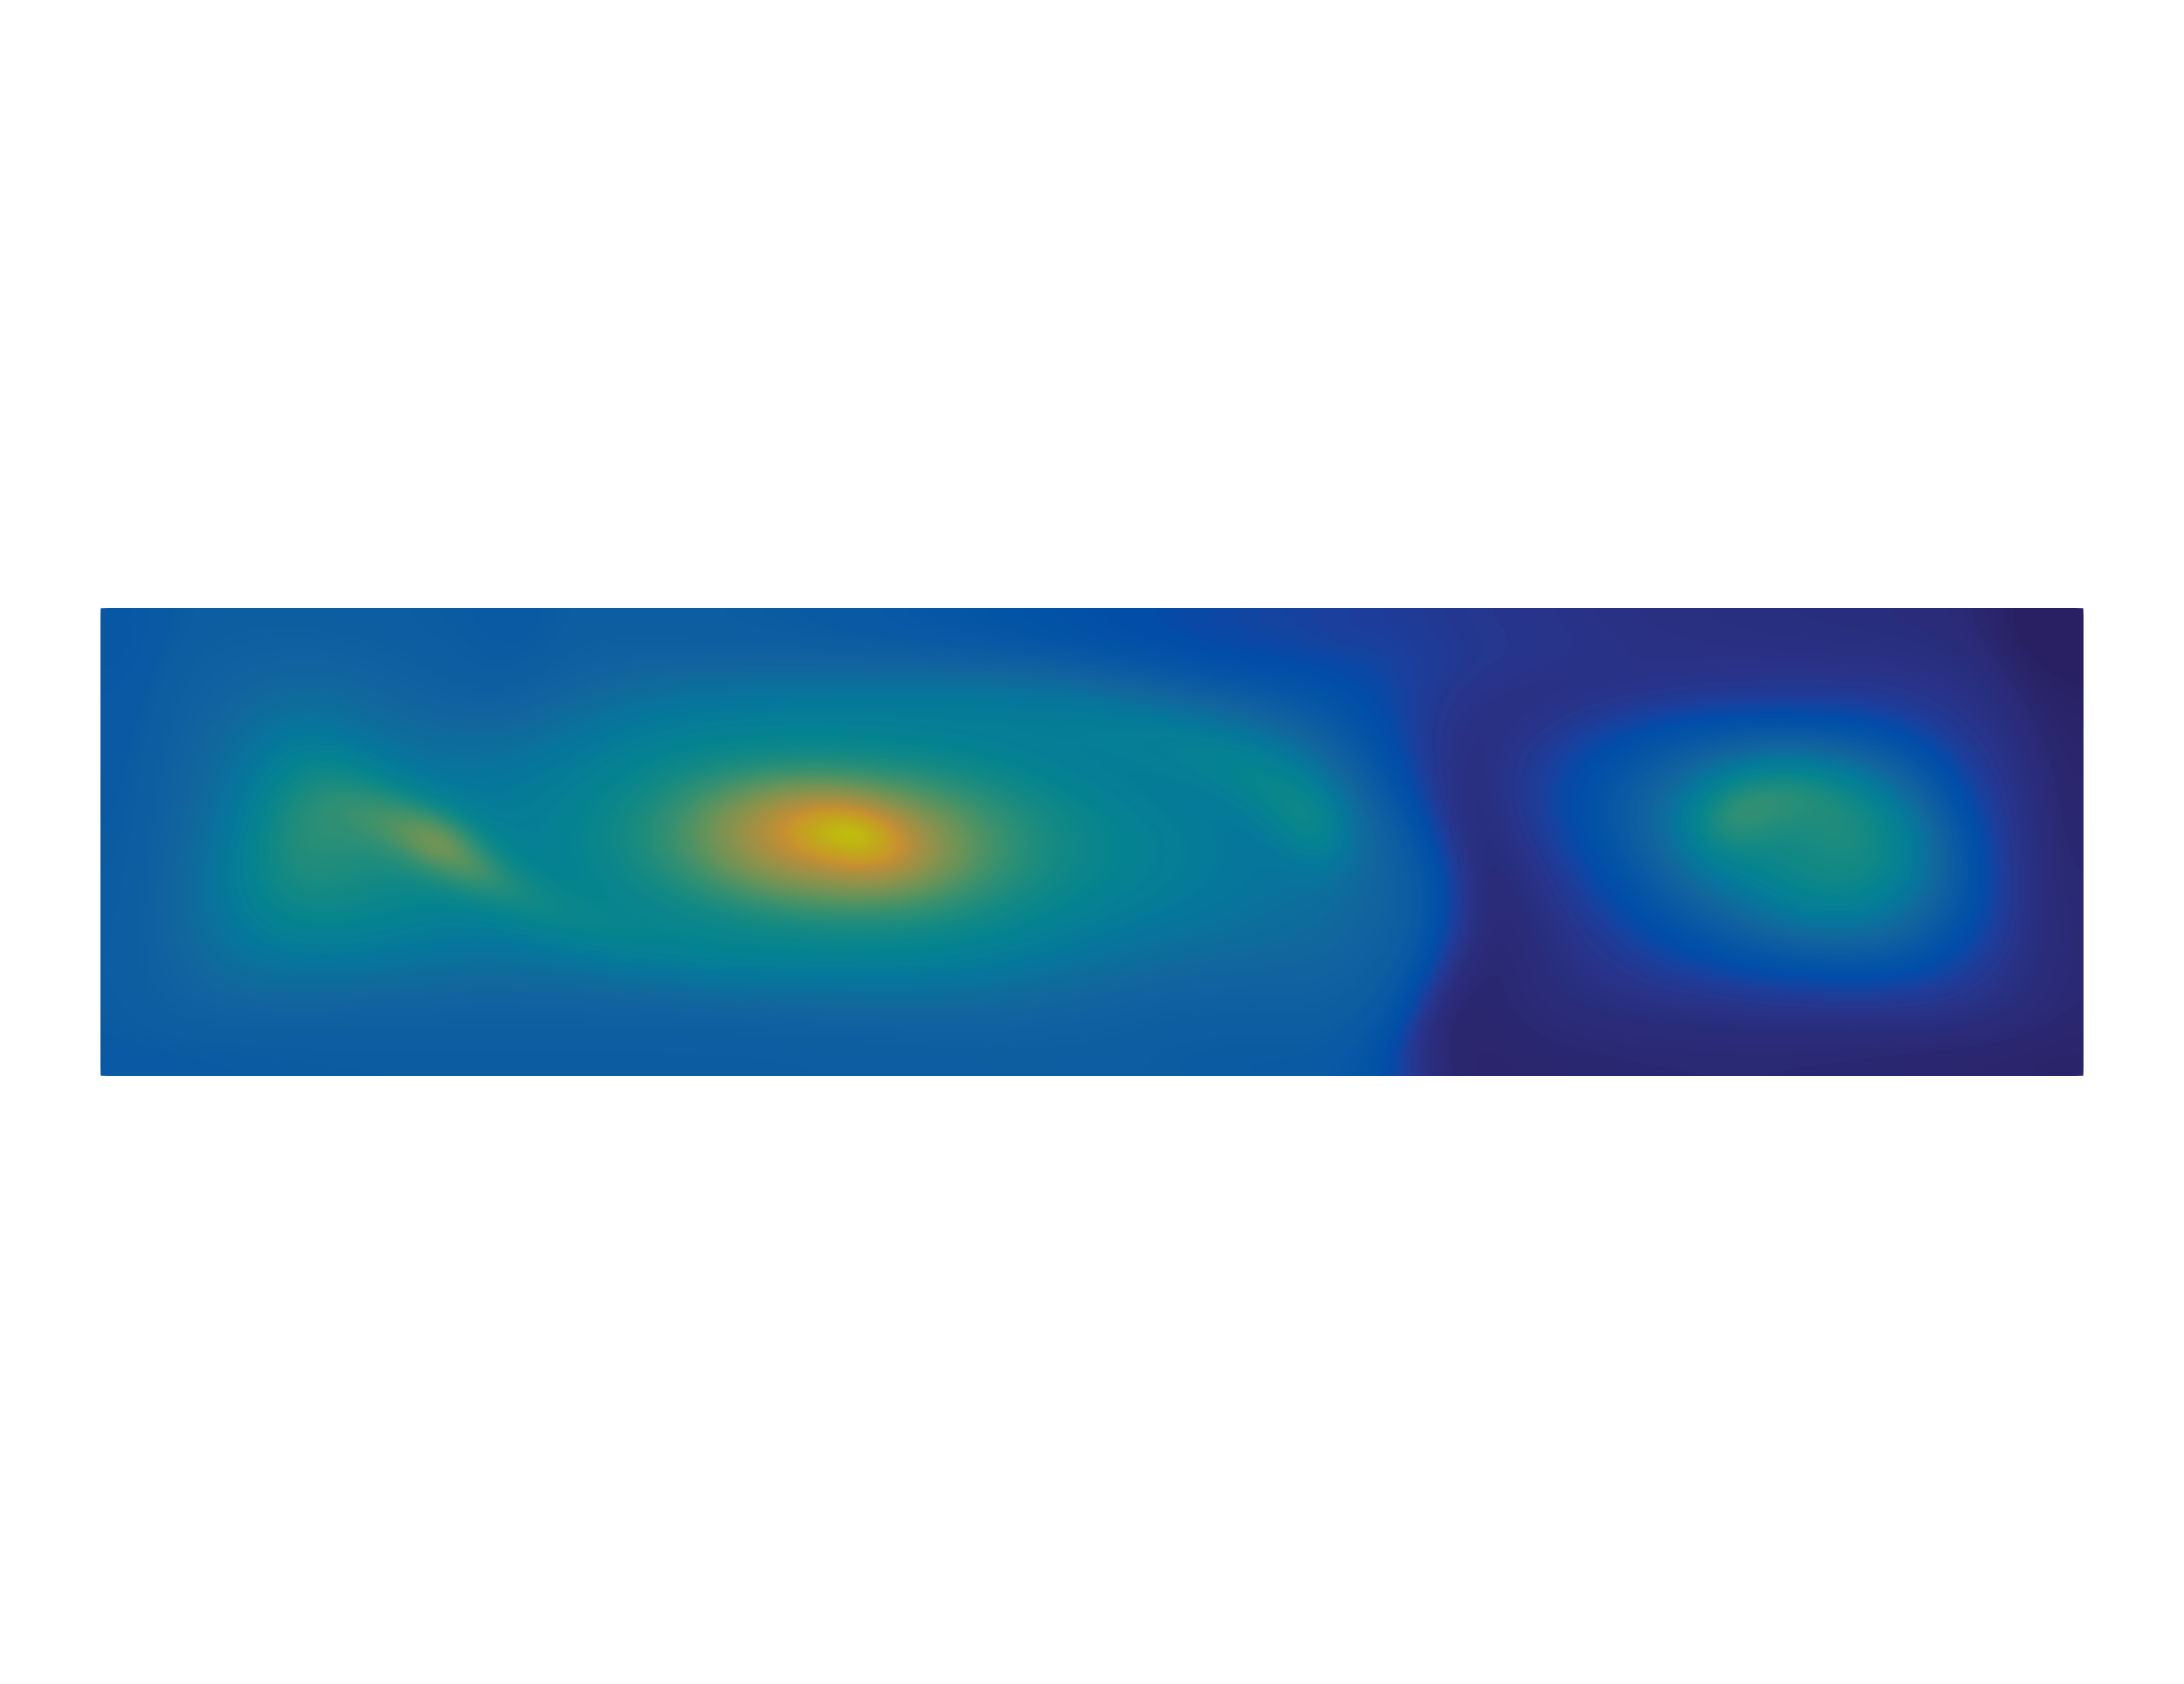
\includegraphics[width=0.99\textwidth]{../media/fourier/application/print/ab-1-1-concentration-harm.png}
        \caption{Anode $(2,1)$ désactivée}
        \label{fig:}
      \end{center}
    \end{subfigure}

    \begin{subfigure}[t]{\textwidth}
      \begin{center}
        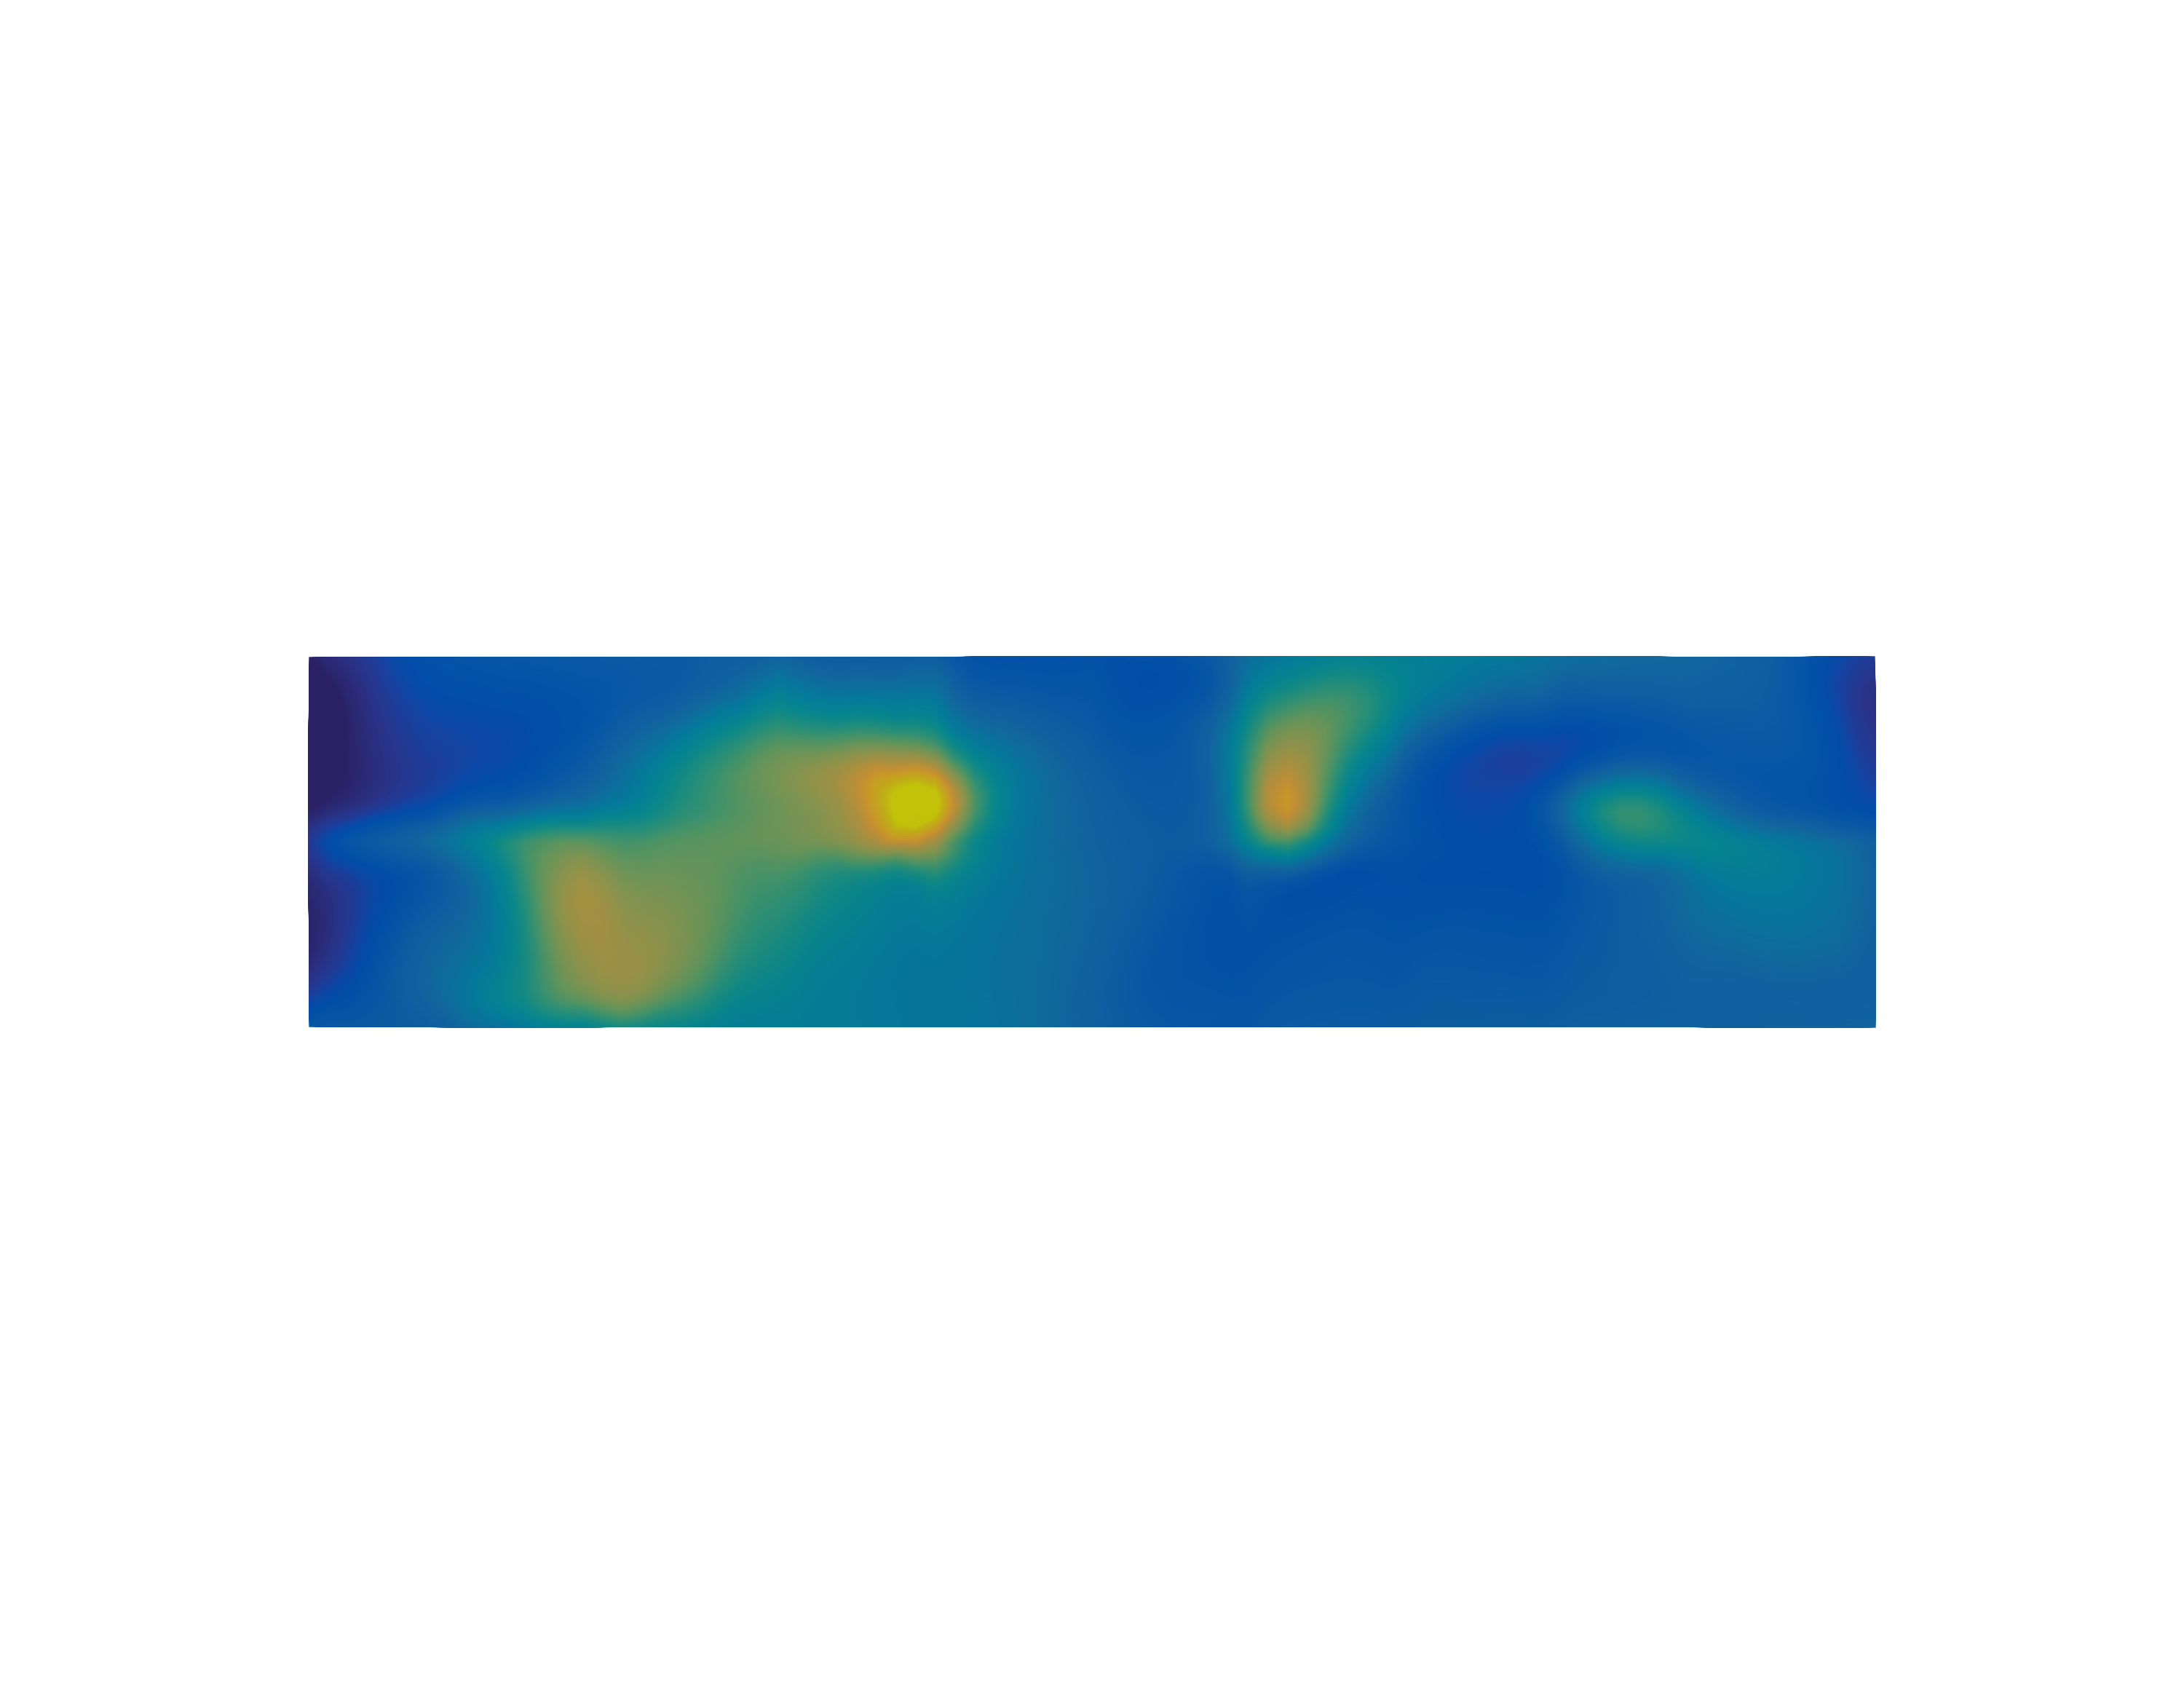
\includegraphics[width=0.99\textwidth]{../media/fourier/application/print/ab-1-2-concentration-acd.png}
        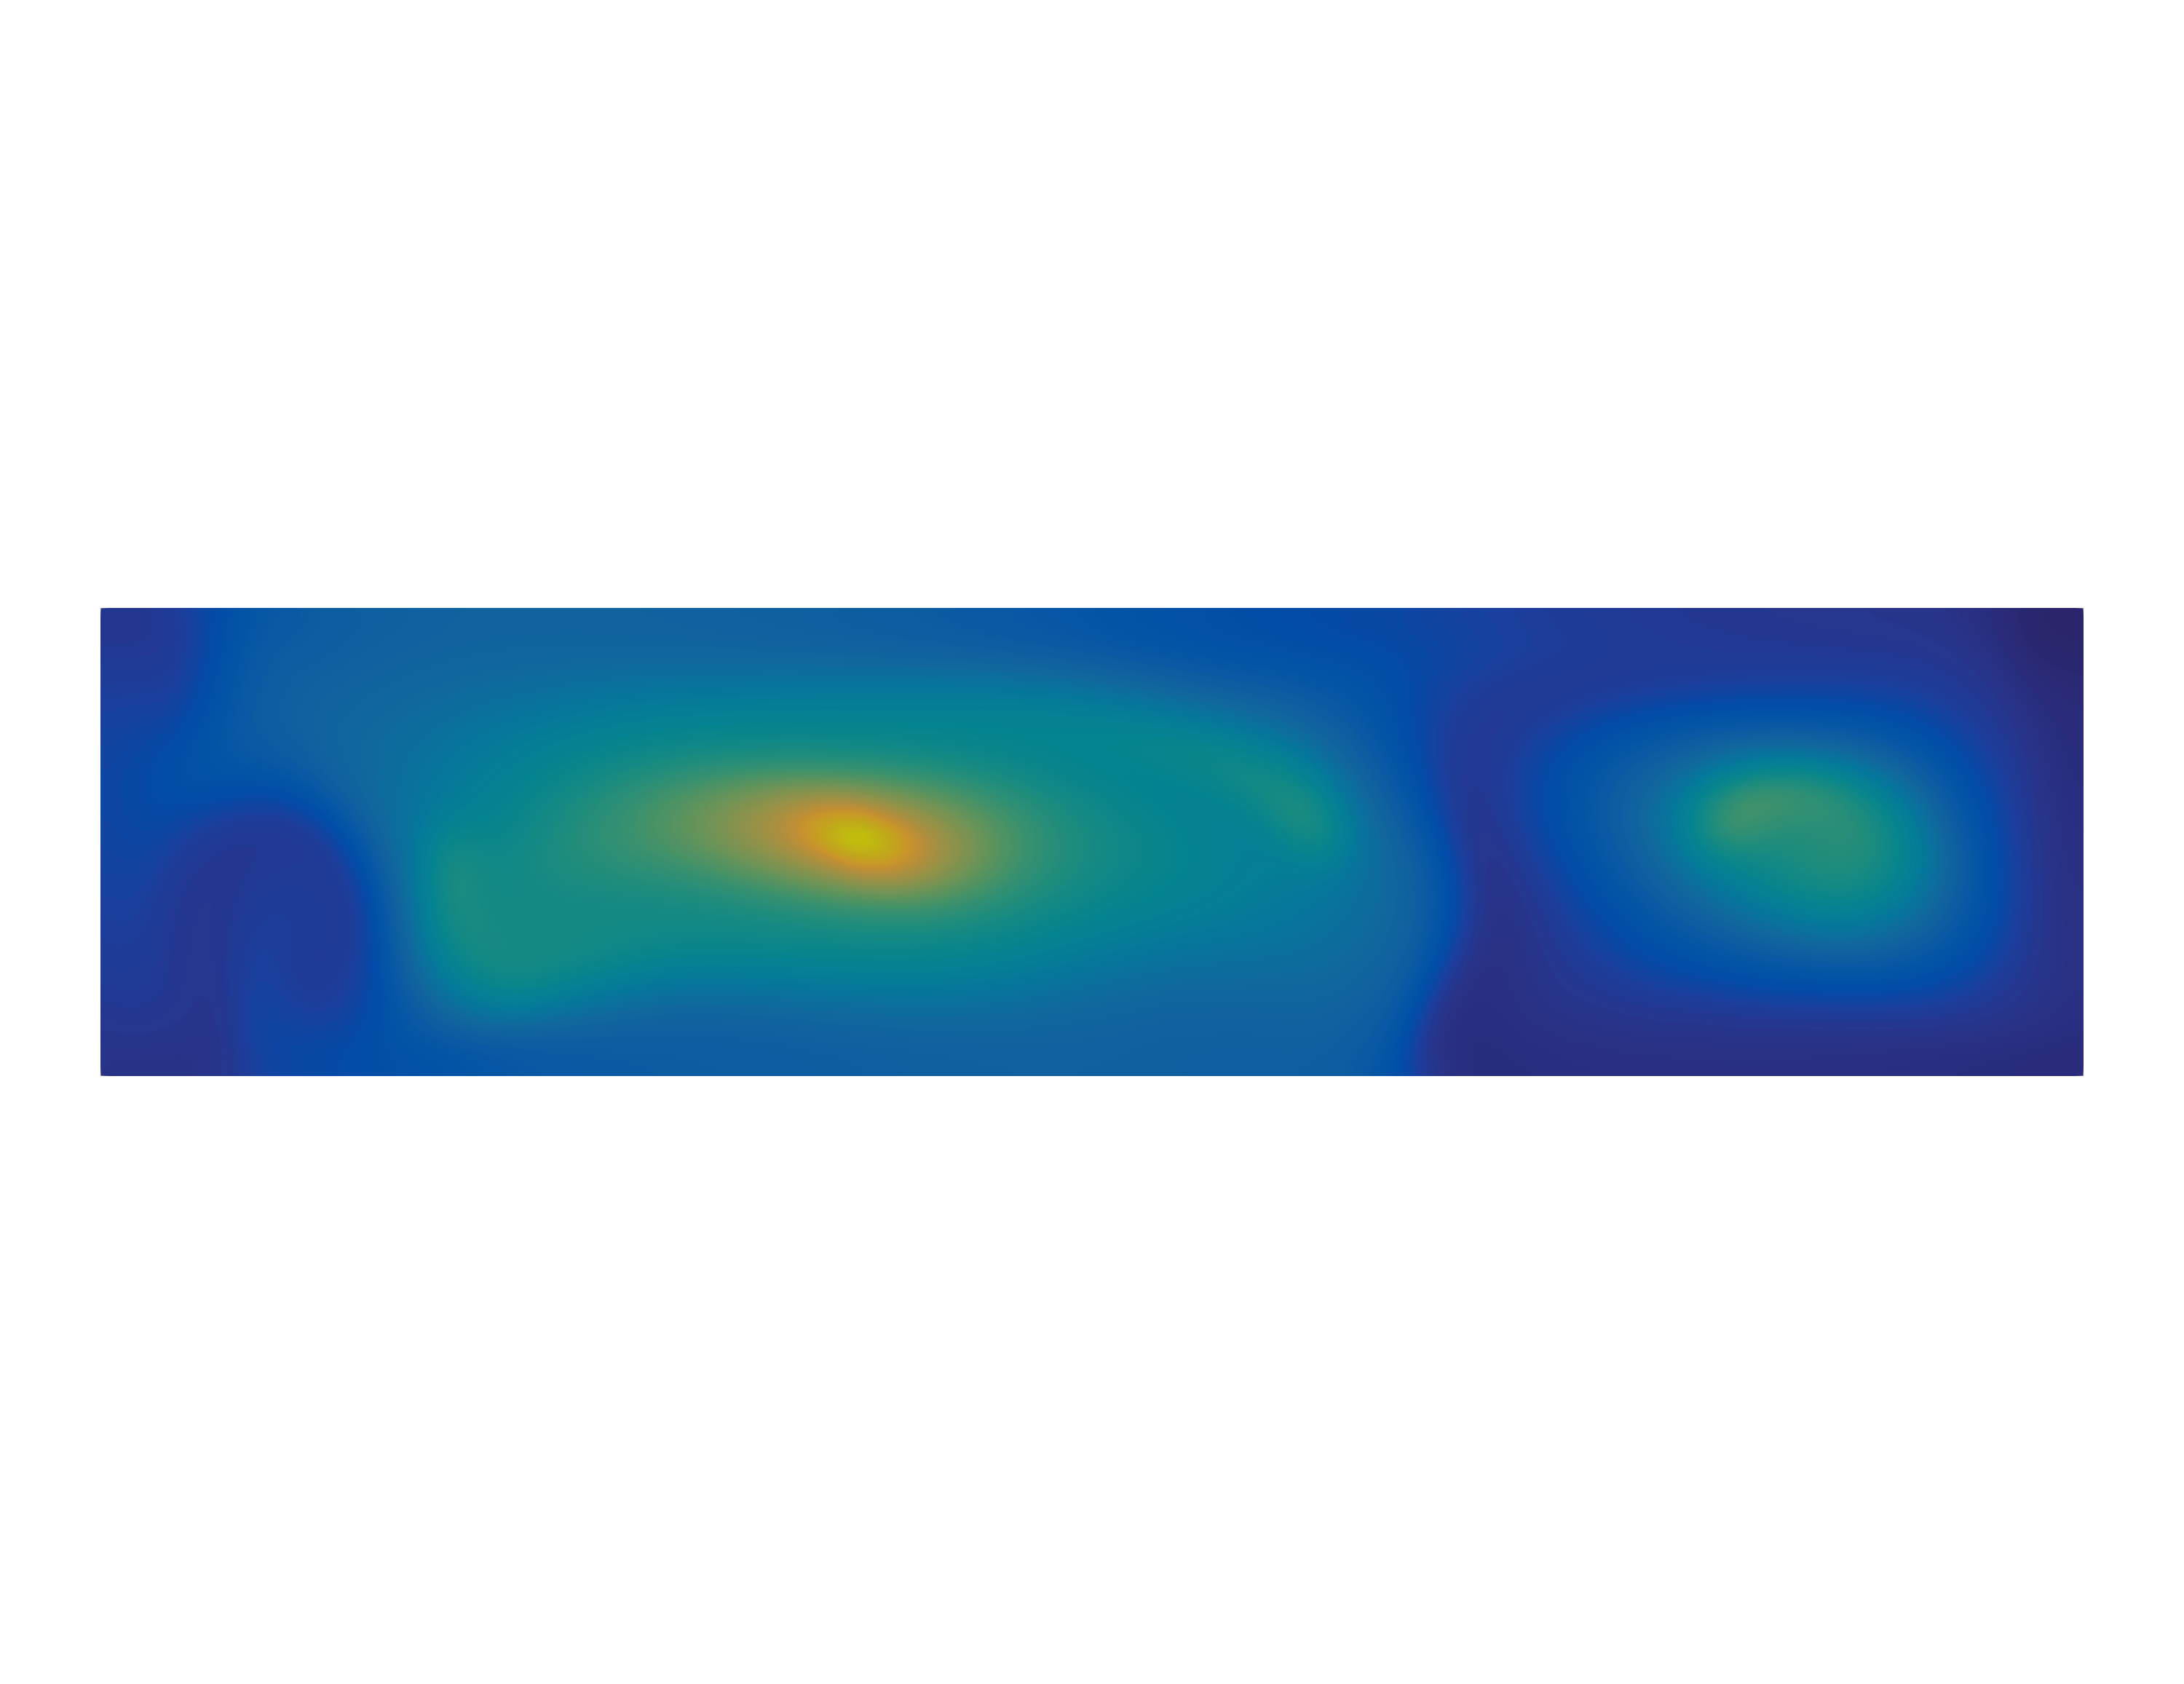
\includegraphics[width=0.99\textwidth]{../media/fourier/application/print/ab-1-2-concentration-harm.png}
        \caption{Anode $(2,2)$ désactivée}
        \label{fig:}
      \end{center}
    \end{subfigure}

    \begin{tikzpicture}
      \begin{axis}[
          colorbar,
          hide axis,
          scale only axis,
          height=0.1\textwidth,
          width=0.5\textwidth,
          colorbar horizontal,
          point meta min=1.73,
          point meta max=6.84,
          colorbar style={
            title=Concentration $c$ [w\%],
            width=4cm,
            height=0.3cm,
            xtick={1.73, 3.0, 5.0, 6.84},
            at={(0.5\textwidth,0.4cm)},
            anchor=north
          }
        ]
        \addplot [] coordinates {(0,0)};
        \node (myfirstpic) at (0,0) {};
      \end{axis}
    \end{tikzpicture}

    \caption{Champ de concentration $c^\mathrm{S3D}$ (haut) et
      $c^\mathrm{SF}$ dans les différentes configurations anodiques.}

    \label{fig:harmonic-concentration-comp-b}
  \end{center}
\end{figure}

Lorsqu'une anodes est désactivée, elle ne conduit plus le courant
électrique, et par conséquent la densité de courant électrique
responsable de la force de Lorentz dans le fluide est fortement
réduite sous l'anode concernée.

On propose d'approximer le champ de force $f$ à partir de $f^0$ en
annulant celle-ci dans la région située sous l'anode désactivée
(figure \ref{fig:anode-deactivation}b.2). Sur la figure
\ref{fig:harmonic-concentration-comp-fc}, on peut comparer les champs
de concentration dans les différentes configurations anodique entre le
modèle S3D et le modèle SF.


\begin{figure}[h!]
  \begin{center}
    \begin{subfigure}[t]{\textwidth}
      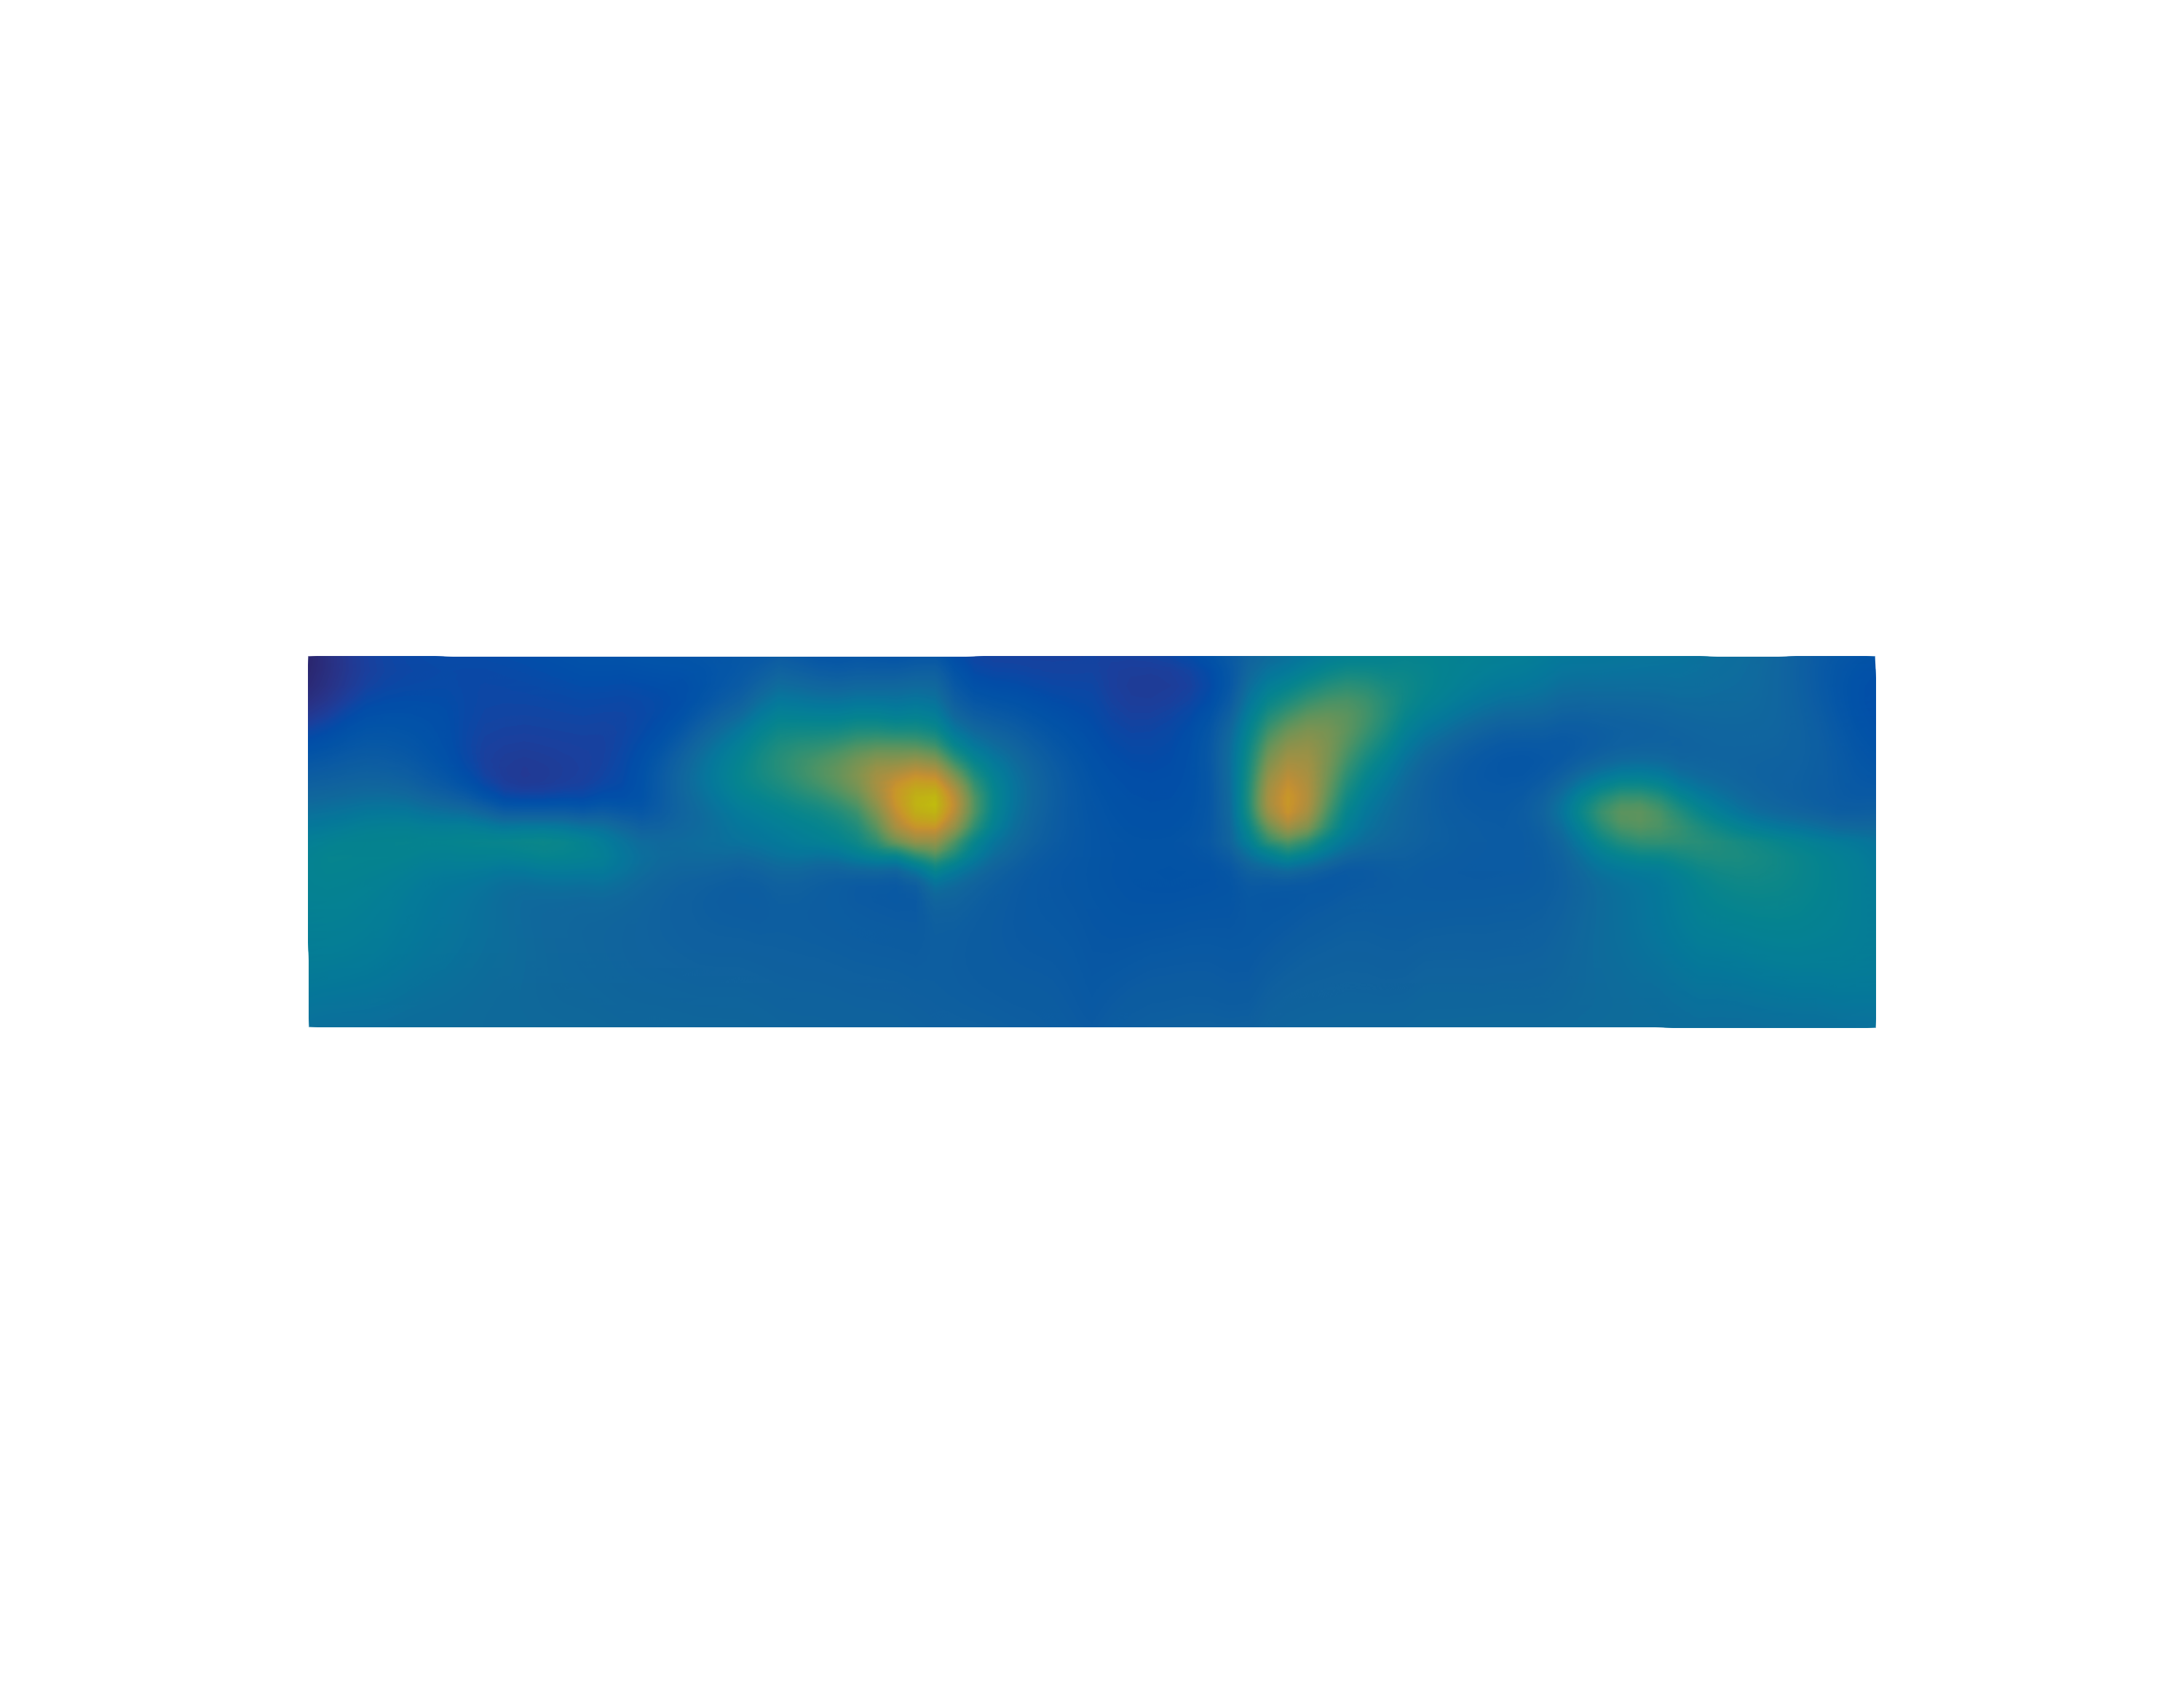
\includegraphics[width=0.99\textwidth]{../media/fourier/application/print/ab-0-1-concentration-acd.png}
      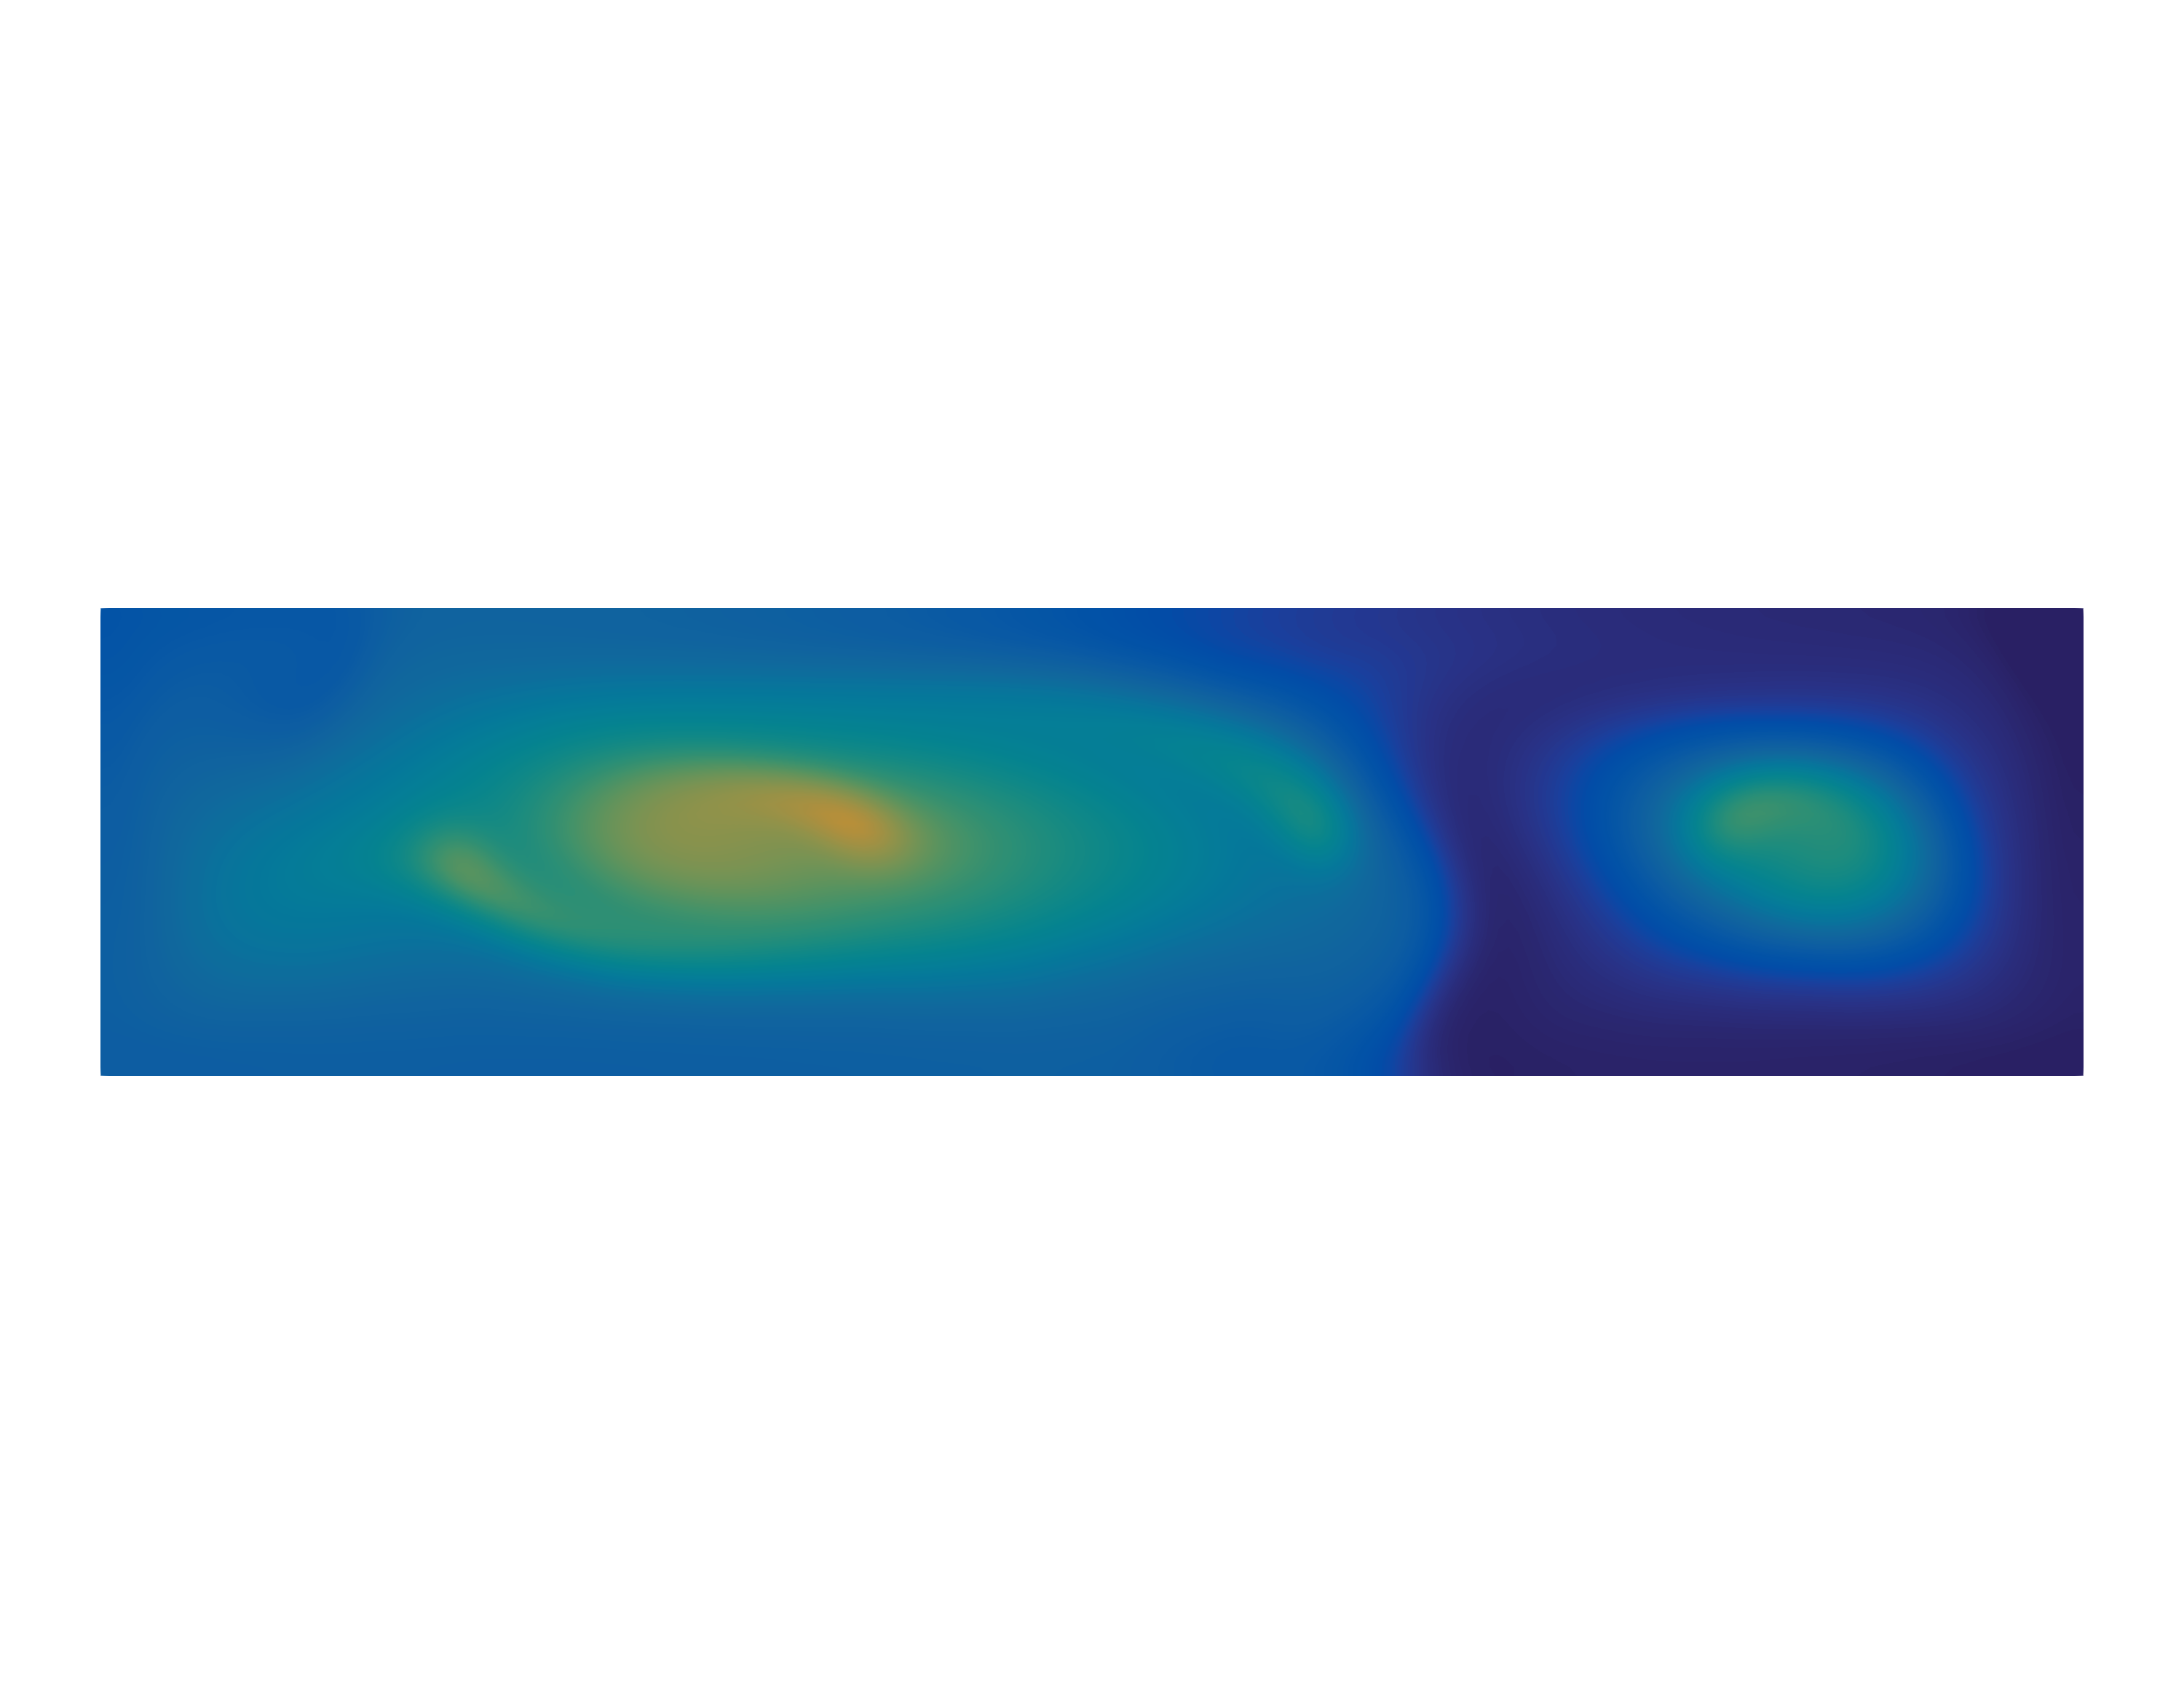
\includegraphics[width=0.99\textwidth]{../media/fourier/application/print/ab-0-1-concentration-harm-fc.png}
      \caption{Anode $(1,1)$ désactivée}
    \end{subfigure}

    \begin{subfigure}[t]{\textwidth}
      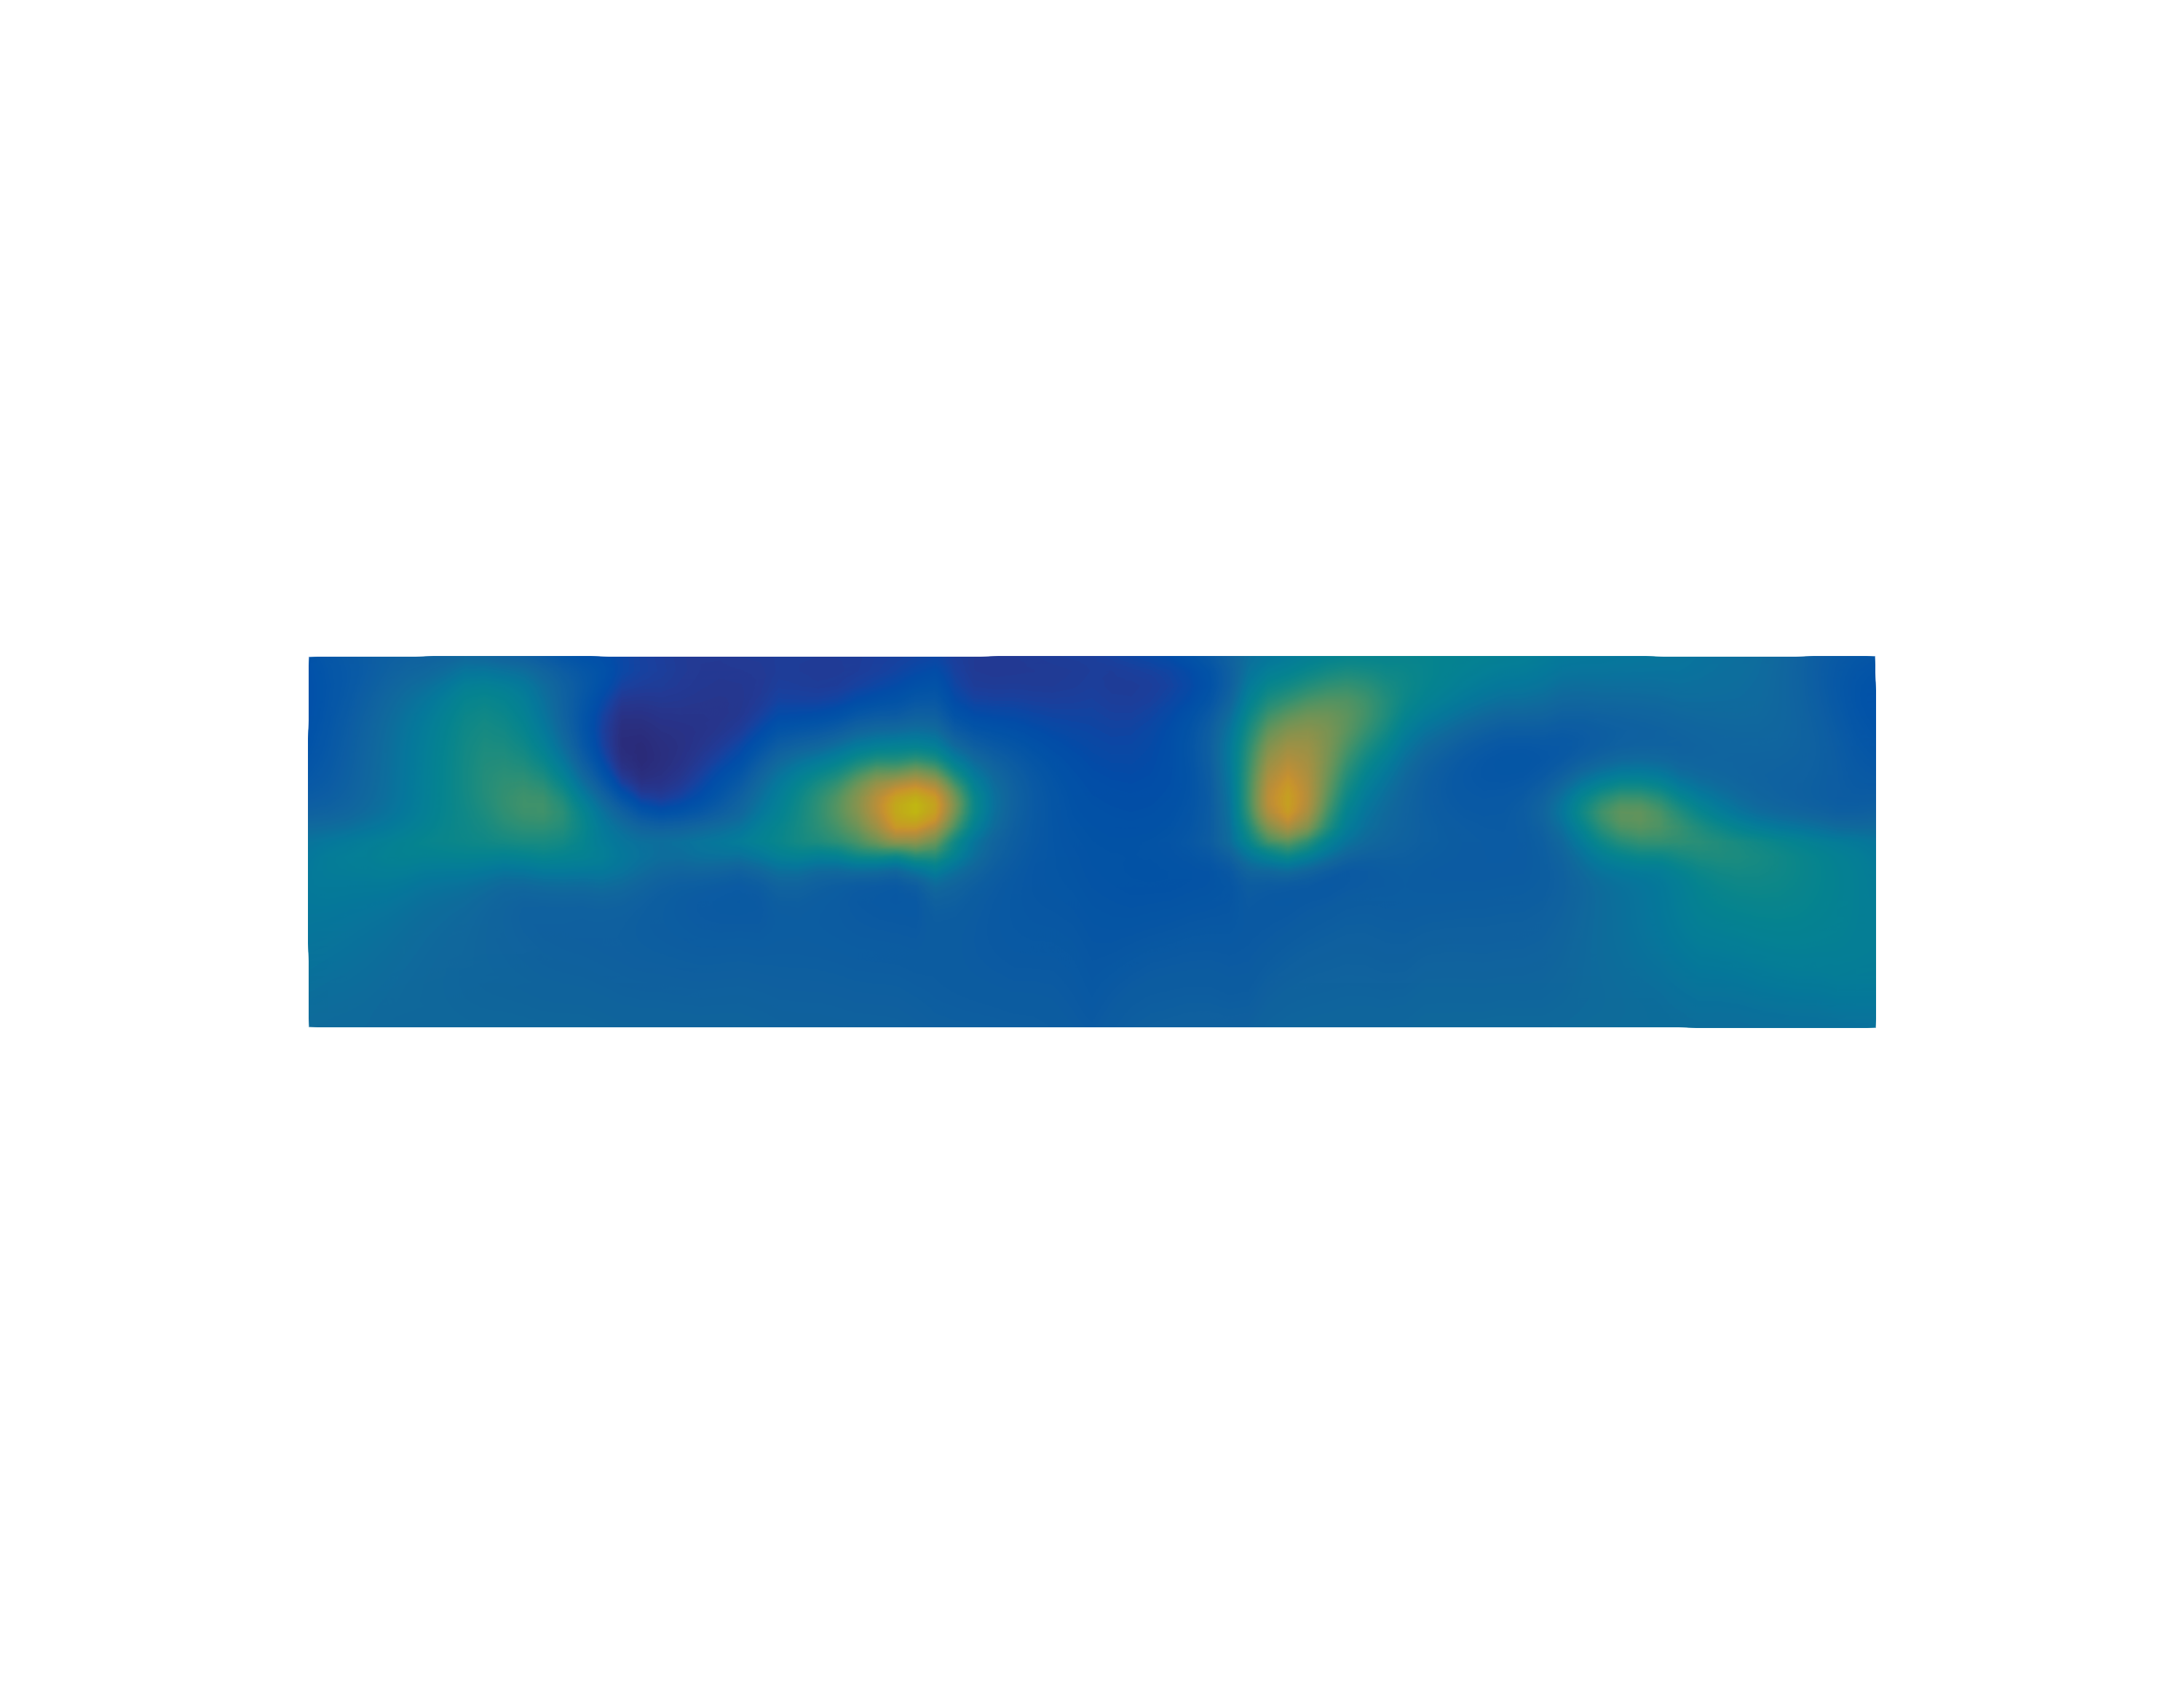
\includegraphics[width=0.99\textwidth]{../media/fourier/application/print/ab-0-2-concentration-acd.png}
      \includegraphics[width=0.99\textwidth]{../media/fourier/application/print/ab-0-2-concentration-harm-fc.png}
      \caption{Anode $(1,2)$ désactivée}
    \end{subfigure}

    \begin{tikzpicture}
      \begin{axis}[
          colorbar,
          hide axis,
          scale only axis,
          height=0.1\textwidth,
          width=0.5\textwidth,
          colorbar horizontal,
          point meta min=1.73,
          point meta max=6.84,
          colorbar style={
            title=Concentration $c$ [w\%],
            width=4cm,
            height=0.3cm,
            xtick={1.73, 3.0, 5.0, 6.84},
            at={(0.3\textwidth,0.4cm)},
            anchor=north
          }
        ]
        \addplot [] coordinates {(0,0)};
        \node (myfirstpic) at (0,0) {};
      \end{axis}
    \end{tikzpicture}

    \caption{Champ de concentration $c_h^\mathrm{S3D}$ dans l'ACD de
      la cuve AP32 (haut), et $c_h^\mathrm{SF}$ sur le plan
      $x_3 = \thickness / 2$ (bas). La force $f$ utilisée
      pour le calcul de $u_h^\mathrm{SF}$  est construite à
      partir de $f^0$, qui est annulée sous l'anode désactivée.}

    \label{fig:harmonic-concentration-comp-fc}
  \end{center}
\end{figure}

\begin{figure}[h!]
  \begin{center}
    \begin{subfigure}[t]{\textwidth}
      \includegraphics[width=0.99\textwidth]{../media/fourier/application/print/ab-1-1-concentration-acd.png}
      \includegraphics[width=0.99\textwidth]{../media/fourier/application/print/ab-1-1-concentration-harm-fc.png}
      \caption{Anode $(2,1)$ désactivée}
    \end{subfigure}

    \begin{subfigure}[t]{\textwidth}
      \includegraphics[width=0.99\textwidth]{../media/fourier/application/print/ab-1-2-concentration-acd.png}
      \includegraphics[width=0.99\textwidth]{../media/fourier/application/print/ab-1-2-concentration-harm-fc.png}
      \caption{Anode $(2,2)$ désactivée}
    \end{subfigure}

    \begin{tikzpicture}
      \begin{axis}[
          colorbar,
          hide axis,
          scale only axis,
          height=0.1\textwidth,
          width=0.5\textwidth,
          colorbar horizontal,
          point meta min=1.73,
          point meta max=6.84,
          colorbar style={
            title=Concentration $c$ [w\%],
            width=4cm,
            height=0.3cm,
            xtick={1.73, 3.0, 5.0, 6.84},
            at={(0.3\textwidth,0.4cm)},
            anchor=north
          }
        ]
        \addplot [] coordinates {(0,0)};
        \node (myfirstpic) at (0,0) {};
      \end{axis}
    \end{tikzpicture}

    \caption{Champ de concentration $c_h^\mathrm{S3D}$ dans l'ACD de la
      cuve AP32 (haut), et $c_h^\mathrm{SF}$ sur le plan $x_3 = \thickness
      / 2$ (bas). La force $f$ utilisée pour le calcul de
      $u_h^\mathrm{SF}$ est construite à partir de $f^0$, qui est annulée
      sous l'anode désactivée.}

    \label{fig:harmonic-concentration-comp-fc}
\end{center}
\end{figure}

\clearpage


\section{Conclusion}
\label{sec:fourier-conclusion}
Dans ce dernier chapitre, nous avons proposé une méthode numérique
pour calculer l'écoulement de fluides dans un domaine
$\Omega = \Lambda\times(0,\thickness)$ de $\mathbb R^3$, basée sur une
décomposition en harmoniques de Fourier des inconnues et des
méthodes d'éléments finis pour chaque coefficients des séries de
Fourier. Cette formulation nécessite d'imposer des conditions
d'adhérence sur les bords verticaux du domaine et des conditions de
glissement total sur les bords horizontaux.

Une caractésistique essentielle de cette méthode est de calculer une
approximation de l'écoulement tridimensionnel en résolvant une
série de problèmes bidimensionnels découplés les uns des autres. Cette
approche devient de plus en plus intéressante lorsque l'épaisseur du
domaine $\thickness$ s'approche de 0. En effet, on observe d'une part
que le temps CPU est essentiellement indépendent de $\thickness$, mais
en plus l'erreur d'approximation diminue lorsque $\thickness$
diminue. C'est un clair avantage par rapport à une méthode
d'éléments finis classiques basée sur un maillage tetraédrique. En
raison de la péjoration du conditionnement des matrice éléments
finis lorsque $\thickness$ tend vers 0, \ie, lorsque le rapport
d'aspect du maillage devient de plus en plus grand, la convergence des
méthodes iteratives devient de plus en plus lente. De plus, l'erreur
d'approximation tend a croître lorsque $\thickness$ diminue.

Cette méthode est donc bien adaptée au calcule d'écoulement de
fluides en couches minces, pour autant que les conditions aux limites
soient adaptées.



\printbibliography[heading=bibintoc]

%%\chapter*{Curriculum Vitae}
\addcontentsline{toc}{chapter}{Curriculum Vitae}
\setboolean{@twoside}{false}
\includepdf[pages=-]{../media/myresume.pdf}


\end{document}
